\documentclass[a4paper]{article}
\usepackage{vntex}
%\usepackage[english,vietnam]{babel}
%\usepackage[utf8]{inputenc}
\usepackage{float}
%\usepackage[utf8]{inputenc}
%\usepackage[francais]{babel}
\usepackage{a4wide,amssymb,epsfig,latexsym,array,hhline,fancyhdr}
\usepackage[normalem]{ulem}
%\usepackage{soul}

\usepackage[makeroom]{cancel}
\usepackage{amsmath}
\usepackage{amsthm}
\usepackage{multicol,longtable,amscd}
\usepackage{diagbox}%Make diagonal lines in tables
\usepackage{booktabs}
\usepackage{alltt}
\usepackage[framemethod=tikz]{mdframed}% For highlighting paragraph backgrounds
\usepackage{caption,subcaption}

\usepackage{lastpage}
\usepackage[lined,boxed,commentsnumbered]{algorithm2e}
\usepackage{enumerate}
\usepackage{color}
\usepackage{graphicx}							% Standard graphics package
\usepackage{array}
\usepackage{tabularx, caption}
\usepackage{multirow}
\usepackage{multicol}
\usepackage{rotating}
\usepackage{graphics}
\usepackage{geometry}
\usepackage{setspace}
\usepackage{epsfig}
\usepackage{tikz}
\usetikzlibrary{arrows,snakes,backgrounds}
\usepackage[unicode]{hyperref}
\hypersetup{urlcolor=blue,linkcolor=black,citecolor=black,colorlinks=true} 
%\usepackage{pstcol} 								% PSTricks with the standard color package

\usepackage[normalem]{ulem}

\newtheorem{theorem}{{\bf Định lý}}
\newtheorem{property}{{\bf Tính chất}}
\newtheorem{proposition}{{\bf Mệnh đề}}
\newtheorem{corollary}[proposition]{{\bf Hệ quả}}
\newtheorem{lemma}[proposition]{{\bf Bổ đề}}
\theoremstyle{definition}
\newtheorem{exer}{Bài toán}

\def\thesislayout{	% A4: 210 × 297
	\geometry{
		a4paper,
		total={160mm,240mm},  % fix over page
		left=30mm,
		top=30mm,
	}
}
\thesislayout

%\usepackage{fancyhdr}
\setlength{\headheight}{40pt}
\pagestyle{fancy}
\fancyhead{} % clear all header fields
\fancyhead[L]{
 \begin{tabular}{rl}
    \begin{picture}(25,15)(0,0)
    \put(0,-8){
\includegraphics[width=8mm, height=8mm]{Images/hcmut.png}}
    %\put(0,-8){\epsfig{width=10mm,figure=hcmut.eps}}
   \end{picture}&
	%
\includegraphics[width=8mm, height=8mm]{hcmut.png} & %
	\begin{tabular}{l}
		\textbf{\bf \ttfamily Trường Đại Học Bách Khoa Tp.Hồ Chí Minh}\\
		\textbf{\bf \ttfamily Khoa Khoa Học \& Kỹ Thuật Máy Tính}
	\end{tabular} 	
 \end{tabular}
}
\fancyhead[R]{
	\begin{tabular}{l}
		\tiny \bf \\
		\tiny \bf 
	\end{tabular}  }
\fancyfoot{} % clear all footer fields
\fancyfoot[L]{\scriptsize \ttfamily Báo cáo Bài tập lớn Cấu trúc Rời rạc cho KHMT (CO1007) - Niên khóa 2019-2020}
\fancyfoot[R]{\scriptsize \ttfamily Trang {\thepage}/\pageref{LastPage}}
\renewcommand{\headrulewidth}{0.3pt}
\renewcommand{\footrulewidth}{0.3pt}


%%%
\setcounter{secnumdepth}{4}
\setcounter{tocdepth}{3}
\makeatletter
\newcounter {subsubsubsection}[subsubsection]
\renewcommand\thesubsubsubsection{\thesubsubsection .\@alph\c@subsubsubsection}
\newcommand\subsubsubsection{\@startsection{subsubsubsection}{4}{\z@}%
                                     {-3.25ex\@plus -1ex \@minus -.2ex}%
                                     {1.5ex \@plus .2ex}%
                                     {\normalfont\normalsize\bfseries}}
\newcommand*\l@subsubsubsection{\@dottedtocline{3}{10.0em}{4.1em}}
\newcommand*{\subsubsubsectionmark}[1]{}
\makeatother

\everymath{\color{blue}}%make in-line maths symbols blue to read/check easily

\sloppy
\captionsetup[figure]{labelfont={small,bf},textfont={small,it},belowskip=-1pt,aboveskip=-9pt}
%space remove between caption, figure, and text
\captionsetup[table]{labelfont={small,bf},textfont={small,it},belowskip=-1pt,aboveskip=7pt}
%space remove between caption, table, and text

%\floatplacement{figure}{H}%forced here float placement automatically for figures
%\floatplacement{table}{H}%forced here float placement automatically for table
%the following settings (11 lines) are to remove white space before or after the figures and tables
%\setcounter{topnumber}{2}
%\setcounter{bottomnumber}{2}
%\setcounter{totalnumber}{4}
%\renewcommand{\topfraction}{0.85}
%\renewcommand{\bottomfraction}{0.85}
%\renewcommand{\textfraction}{0.15}
%\renewcommand{\floatpagefraction}{0.8}
%\renewcommand{\textfraction}{0.1}
\setlength{\floatsep}{5pt plus 2pt minus 2pt}
\setlength{\textfloatsep}{5pt plus 2pt minus 2pt}
\setlength{\intextsep}{10pt plus 2pt minus 2pt}

\thesislayout

\everymath{\displaystyle \color{blue}}

\begin{document}

\begin{titlepage}
\begin{center}
ĐẠI HỌC QUỐC GIA THÀNH PHỐ HỒ CHÍ MINH \\
TRƯỜNG ĐẠI HỌC BÁCH KHOA \\
KHOA KHOA HỌC \& KỸ THUẬT MÁY TÍNH 
\end{center}

\vspace{1cm}

\begin{figure}[h!]
\begin{center}

\includegraphics[width=3cm]{Images/hcmut.png}
\end{center}
\end{figure}

\vspace{1cm}


\begin{center}
\begin{tabular}{c}
\multicolumn{1}{c}{\textbf{{\Large CẤU TRÚC RỜI RẠC CHO KHMT (CO1007)}}}\\
~~\\
\hline
\\
% \multicolumn{1}{l}{\textbf{{\Large Đề bài tập lớn cho Nhóm $n$}}}\\
% \\
% \textbf{{\Huge Thống kê mô tả và}} \\
% \textbf{{\Huge Xác suất rời rạc với R}}\\
\textbf{\large Ứng dụng thống kê} \\
\textbf{\large khảo sát kết quả của bài tập online cho phép nộp bài nhiều lần}
\\
\hline
\end{tabular}
\end{center}

\vspace{1.5cm}

\begin{table}[h]
\begin{tabular}{rrl}
\hspace{5 cm} & GVHD: & Huỳnh Tường Nguyên\\
\hspace{5 cm} &  & Trần Tuấn Anh\\
\hspace{5 cm} &  & Nguyễn Ngọc Lễ\\

& Nhóm: & 25\\

& SV thực hiện: & Tô Hòa -- 1910198 \\
& & Trương Vĩnh Phước -- 1910473 \\
& & Nguyễn Huỳnh Đức -- 1910137 \\
& & Nguyễn Hoàng Trung -- 1910644 \\
& & Ngô Lê Quốc Dũng -- 1910101 \\
& & Lại Đức Anh Khoa -- 1910265 \\

\end{tabular}
\end{table}
\vspace{3.5cm}
\begin{center}
{\footnotesize Tp. Hồ Chí Minh, Tháng 06/2020}
\end{center}
\end{titlepage}


%\thispagestyle{empty}

\newpage
\tableofcontents
\newpage


\section{Động cơ nghiên cứu}\label{motivation}
$\indent$Trong mùa dịch Covid-19, trường Đại học Bách Khoa, ĐHQG-HCM đã triển khai giảng dạy trực tuyến và yêu cầu sinh viên thực hiện các bài tập nhỏ để thu nhận phản hồi về việc học tập và hiểu biết của các bạn thông qua các tài nguyên online được cung cấp.

Phân tích \& thống kê dữ liệu qua các lần nộp bài của sinh viên không những giúp giáo viên có những hướng đúng trong việc phát hiện ra những kiến thức mà sinh viên chưa chắc chắn, cũng như có hướng để cải thiện bổ sung phần học liệu trong tương lai để phù hợp với hơn người học.

\section{Mục tiêu}\label{objective}
$\indent$Khai phá dữ liệu từ hệ thống nộp bài online có ý nghĩa quan trọng trong việc đánh giá chất lượng của sinh viên. Ngoài ra, những đánh giá kết quả nộp bài của từng sinh viên, hay từng bài tập sẽ góp phần xác định những điểm mạnh, điểm yếu của sinh viên để giáo viên có phương pháp phù hợp trong việc cải thiện kỹ năng của sinh viên.

Trong bài tập lớn này, các sinh viên sẽ bắt đầu với các bài toán thống kê đơn giản từ những dữ liệu được cung cấp. Qua đó, các em sẽ tìm ra những con số thú vị, có ý nghĩa đối với các dữ liệu thực tế trong quá khứ của hệ thống chấm bài online. Những kết quả mà các em tìm ra sẽ là bước khởi đầu cho việc khai phá nguồn dữ liệu của hệ thống sau này, nhằm đạt tới mục tiêu nâng cao kỹ năng lập trình, kỹ năng giải quyết vấn đề cho người học cũng như hướng tới mục tiêu cao hơn khi tích hợp với các hệ thống quản lý và cải thiện chất lượng dạy và học.

\section{Mô tả dữ liệu}\label{sec:dataset}
$\indent$Đính kèm đề bài tập lớn là 24 files {\bf filename.xlsx} (``CO1007\_TV\_HK192-Quiz...xlsx'') trong đó chứa thông tin về điểm qua các lần nộp các bài Quiz của các sinh viên trên BKEL. Thông tin bài tập lớn:
\begin{enumerate}
	\item $tid$ là mã số bài tập (gồm có 24 file dữ liệu nên mã bài tập là các số từ 1 đến 24 thay cho tên file)
	\item \textcolor{blue}{Mã số ID} ta gọi là $uid$ là mã số định danh sinh viên nộp bài, mỗi sinh viên có một \it{mã số id} duy nhất và không trùng với một \it{ mã số id} của các sinh viên khác	    
	\item \textcolor{blue}{Tình trạng}: Đã hoàn thành hoặc chưa bao giờ gởi
	\item \textcolor{blue}{Đã bắt đầu vào lúc}, \textcolor{blue}{Đã hoàn thành}: Thời gian theo dạng ``d B Y I:M p'' là thời gian bắt đầu và kết thúc làm bài. Trong đó, ``e'' là ngày (1..31)  ``B'' tên tháng đầy đủ, ``Y'' là năm (0..9999),``I'' là giờ (01..12), ``M'' là phút (00–59), ``p'' chỉ định AM/PM
	\item \textcolor{blue}{Thời gian thực hiện}: Khoảng thời gian làm bài 
	\item \textcolor{blue}{Điểm/10}: Tổng số điểm của các quiz cộng lại thấp nhất là 0, tối đa là 10
    \item \textcolor{blue}{Q.i/1} là điểm số của bài quiz chỉ 0 hoặc 1.
\end{enumerate}

\section{Nhiệm vụ}\label{requirement} 
\subsection{Thông tin chung}
$\indent$Nhóm: 25\\[6pt]
$\indent$Mã đề: $MD = 2907$\\[6pt]
$\indent$Bài tập cần làm: \textbf{1, 2, 3, 4, 5, 7, 9}\\[6pt]
$\indent$Bài tập làm thêm: \textbf{12}\\[6pt]
$\indent$Các file cần xử lý:
\begin{itemize}
	\item {\bf File 1:} CO1007\_TV\_HK192-Quiz 1.4-điểm.xlsx
	\item {\bf File 2:} CO1007\_TV\_HK192-Quiz 1.5-điểm.xlsx	
	\item {\bf File 3:} CO1007\_TV\_HK192-Quiz 3.3-điểm.xlsx
	\item {\bf File 4:} CO1007\_TV\_HK192-Quiz 4.2-điểm.xlsx
\end{itemize}
\subsection{Đọc dữ liệu}
$\indent$ Dữ liệu được đọc từ các file excel được lưu trữ trong một dataframe có tên là $data$. Dữ liệu trong $data$ bào gồm:
\begin{itemize}
    \item Cột \textcolor{blue}{ID} lưu trữ tất cả \textcolor{blue}{Mã số ID} của các lần nộp bài.
    \item Cột \textcolor{blue}{Status} lưu trữ \textcolor{blue}{Tình trạng} của các lần nộp bài bao gồm: \textit{Done} đại diện cho \textit{Đã hoàn thành} và \textit{Not done} đại diện cho \textit{Chưa bào giờ gửi}.
    \item Data frame \textcolor{blue}{Start} gồm 5 cột: \textcolor{blue}{Start.day}, \textcolor{blue}{Start.month}, \textcolor{blue}{Start.year}, \textcolor{blue}{Start.hour} và \textcolor{blue}{Start.minute} lưu trữ thời gian (ngày, tháng, năm, giờ và phút) của \textcolor{blue}{Đã bắt đầu vào lúc} (thời gian thực hiện bài thi).
    \item Data frame \textcolor{blue}{Finish} gồm 5 cột: \textcolor{blue}{Finish.day}, \textcolor{blue}{Finish.month}, \textcolor{blue}{Finish.year}, \textcolor{blue}{Finish.hour} và \textcolor{blue}{Finish.minute} lưu trữ thời gian (ngày, tháng, năm, giờ và phút) của \textcolor{blue}{Đã hoàn thành} (thời gian nộp bài).
    \item Cột \textcolor{blue}{Duration} lưu trữ \textcolor{blue}{Thời gian thực hiên} theo đơn vị giây.
    \item Cột \textcolor{blue}{Total} lưu trữ \textcolor{blue}{Điểm/10} (Tổng điểm của các Quiz).
    \item 10 cột \textcolor{blue}{Q1} đến \textcolor{blue}{Q10} lưu trữ \textcolor{blue}{Q.i/1} (điểm số của bài Quiz).
\end{itemize}
\subsection{Xử lý dữ liệu}
%%%%%%%%%%%%%%%%%%%%%%%%%%%%%%%%%%%%%%%%%%%%%%%%%%%%%%%%%%%%%%%%%%%%%%%%%%%%%%%%%%%%%%%%%%%%%%%%%%%%%%%%
%         ->       Bai 1
%%%%%%%%%%%%%%%%%%%%%%%%%%%%%%%%%%%%%%%%%%%%%%%%%%%%%%%%%%%%%%%%%%%%%%%%%%%%%%%%%%%%%%%%%%%%%%%%%%%%%%%%
\addcontentsline{toc}{subsubsection}{Bài 1: Xác định số lượng sinh viên trong tập mẫu}
\subsubsection*{Bài 1: Xác định số lượng sinh viên trong tập mẫu}
\bf Kiến thức chuẩn bị\normalfont
\begin{itemize}
    \item Cách giải truyền thống:
    \begin{itemize}
        \item Mỗi sinh viên có một mã số sinh viên (MSSV) riêng, do đó số lượng sinh viên sẽ bằng số lượng phần từ của tập hợp các mã số sinh viên.
    \end{itemize}
\end{itemize}
\bf Hiện thực trên R\normalfont
\begin{itemize}
    \item Ý tưởng thực hiện:
    \begin{itemize}
        \item Ta sử dụng hàm $unique()$ để lấy tập giá trị của tập mã số sinh viên và sử dụng hàm $length()$ để lấy số lượng tâp giá trị đó.
        \begin{center}
            \begin{tabular}{p{13cm}}
                \texttt{student\_num <- length(unique(data\$ID))}\\
            \end{tabular}
        \end{center}
    \end{itemize}
    \item Kết quả: 
    \begin{itemize}
        \item Số lượng sinh viên ứng với mỗi file:
        \begin{center}
            \begin{tabular}{l l}
                 \texttt{"CO1007\_TV\_HK192-Quiz 1.4-điểm.xlsx"} & 344 sinh viên\\ 
                 \texttt{"CO1007\_TV\_HK192-Quiz 1.5-điểm.xlsx"} & 343 sinh viên\\ 
                 \texttt{"CO1007\_TV\_HK192-Quiz 3.3-điểm.xlsx"} & 280 sinh viên\\ 
                 \texttt{"CO1007\_TV\_HK192-Quiz 4.2-điểm.xlsx"} & 260 sinh viên\\ 
            \end{tabular}
        \end{center}
    \end{itemize}
\end{itemize}
%%%%%%%%%%%%%%%%%%%%%%%%%%%%%%%%%%%%%%%%%%%%%%%%%%%%%%%%%%%%%%%%%%%%%%%%%%%%%%%%%%%%%%%%%%%%%%%%%%%%%%%%
%         ->       Bai 2
%%%%%%%%%%%%%%%%%%%%%%%%%%%%%%%%%%%%%%%%%%%%%%%%%%%%%%%%%%%%%%%%%%%%%%%%%%%%%%%%%%%%%%%%%%%%%%%%%%%%%%%%
\addcontentsline{toc}{subsubsection}{Bài 2: Nhóm câu hỏi liên quan đến điểm số của các sinh viên}
\subsubsection*{Bài 2: Nhóm câu hỏi liên quan đến điểm số của các sinh viên}
\begin{enumerate}[a)]
    %Cau a
    \bf\item {Xác định điểm số là điểm tổng của các bài làm với mỗi câu hỏi đơn vị đều có điểm tối đa là 1 điểm.}\\[6pt]
    \bf Kiến thức chuẩn bị\normalfont
    \begin{itemize}
        \item Cách giải truyền thống:
        \begin{itemize}
            \item Ta tính tổng tất cả các giá trị tổng điểm của các bài làm trong tập dữ liệu.
        \end{itemize}
    \end{itemize}
    \bf Hiện thực trên R\normalfont
    \begin{itemize}
        \item Ý tưởng thực hiện:
        \begin{itemize}
            \item Ta sử dụng hàm $sum()$ để tính tổng điểm của tất cả các bài làm.
        \end{itemize}
        \item Kết quả:
        \begin{itemize}
            \item Điểm tổng của tất cả các bài làm của mỗi file:
            \begin{center}
                \begin{tabular}{l c}
                     \texttt{"CO1007\_TV\_HK192-Quiz 1.4-điểm.xlsx"} & 5512.25\\
                     \texttt{"CO1007\_TV\_HK192-Quiz 1.5-điểm.xlsx"} & 5668.5\\
                     \texttt{"CO1007\_TV\_HK192-Quiz 3.3-điểm.xlsx"} & 3410\\
                     \texttt{"CO1007\_TV\_HK192-Quiz 4.2-điểm.xlsx"} & 4406
                \end{tabular}
            \end{center}
        \end{itemize}   
    \end{itemize}
    %Cau b
    \bf\item {Xác định điểm số thấp nhất}\\[6pt]
    \bf Kiến thức chuẩn bị\normalfont
    \begin{itemize}
        \item Cách giải truyền thống:
        \begin{itemize}
            \item Từ danh sách các bài nộp, ta chọn ra giá trị điểm số thấp nhất.
        \end{itemize}
    \end{itemize}
    \bf Hiện thực trên R\normalfont
    \begin{itemize}
        \item Ý tưởng thực hiện:
        \begin{itemize}
            \item Ta dùng hàm $min()$ để tìm giá trị nhỏ nhất của 1 vector. Ở đây, $K$ là một data frame đã lọc ra các dữ liệu thừa hay lỗi.
            \begin{center}
                \begin{tabular}{p{13cm}}
                    \texttt{Least.Total <- min(K[,6])}
                \end{tabular}
            \end{center}
        \end{itemize}
        \item Kết quả:
        \begin{itemize}
            \item Điểm số thấp nhất của mỗi file:
            \begin{center}
                \begin{tabular}{l c}
                     \texttt{"CO1007\_TV\_HK192-Quiz 1.4-điểm.xlsx"} & 4.5 điểm\\
                     \texttt{"CO1007\_TV\_HK192-Quiz 1.5-điểm.xlsx"} & 0.5 điểm\\
                     \texttt{"CO1007\_TV\_HK192-Quiz 3.3-điểm.xlsx"} & 0 điểm\\
                     \texttt{"CO1007\_TV\_HK192-Quiz 4.2-điểm.xlsx"} & 0 điểm
                \end{tabular}
            \end{center}
        \end{itemize}
    \end{itemize}
    %Cau c
   \bf\item {Xác định danh sách các sinh viên có ít nhất một bài có số điểm thấp nhất}\\[6pt]
    \bf Kiến thức chuẩn bị\normalfont
    \begin{itemize}
        \item Cách giải truyền thống:
        \begin{itemize}
            \item Ta đã biết được số điểm thấp nhất qua câu b, nên ta có thể lập danh sách các sinh viên có ít nhất một bài toán có số điểm thấp nhất dựa vào giá trị vừa tìm được.
        \end{itemize}
    \end{itemize}
    \bf Hiện thực trên R\normalfont
    \begin{itemize}
        \item Ý tưởng thực hiện:
        \begin{itemize}
            \item Dùng hàm subset để trích ra một data frame mới với yêu cầu là có số điểm Total bằng số điểm thấp nhất.
            \begin{center}
                \begin{tabular}{p{13cm}}
                    \texttt{List.Least.Total <- subset(K, K\$Total == Least.Total)}
                \end{tabular}
            \end{center}
            \item Tuy nhiên nếu chỉ lọc như thế này có khả năng một sinh viên có thể xuất hiện nhiều hơn một lần trong danh sách này, nên ta dùng thêm hai hàm $match()$ và $unique()$.
            \begin{center}
                \begin{tabular}{p{13cm}}
                    \texttt{List.Least.Total.Unique <- List.Least.Total[match(unique( List.Least.Total\$ID), List.Least.Total\$ID),]}
                \end{tabular}
            \end{center}
        \end{itemize}
        \item Kết quả:
        \begin{itemize}
            \item Danh sách các sinh viên có ít nhất một bài có điểm số thấp nhất của mỗi file:
            \begin{center}
                \begin{tabular}{l c c c c c c c}
                     \texttt{"CO1007\_TV\_HK192-Quiz 1.4-điểm.xlsx"} & 1913315\\
                     \texttt{"CO1007\_TV\_HK192-Quiz 1.5-điểm.xlsx"} & 1915775\\
                     \texttt{"CO1007\_TV\_HK192-Quiz 3.3-điểm.xlsx"} & 1914661\\
                     \texttt{"CO1007\_TV\_HK192-Quiz 4.2-điểm.xlsx"} & 1914661
                \end{tabular}
            \end{center}
        \end{itemize}
    \end{itemize}
    %Cau d
    \bf\item {Xác định phổ theo số lần nộp bài của các sinh viên có ít nhất một bài có số điểm thấp nhất}\\[6pt]
    \bf Kiến thức chuẩn bị\normalfont
    \begin{itemize}
        \item Cách giải truyền thống:
        \begin{itemize}
            \item Từ danh sách các bạn sinh viên có ít nhất một bài có số điểm thấp nhất và danh sách ban đầu, ta tạo được một danh sách mới với các bạn sinh viên có it nhất một bài có số điểm thấp nhất và số lần làm bài của các bạn ấy.
        \end{itemize}
    \end{itemize}
    \bf Hiện thực trên R\normalfont
    \begin{itemize}
        \item Ý tưởng thực hiện:
        \begin{itemize}
            \item Ta tạo một dataframe mới (gọi tạm là $List.Least.Total2$) là một subset của dataframe ban đầu kèm xét thêm điều kiện là ID phải tồn tại trong dataframe $List.Least.Total.Unique$ (tức là các sinh viên có ít nhất một bài có số điểm thấp nhất).
            \begin{center}
                \begin{tabular}{p{13cm}}
                    \texttt{List.Least.Total2 <- subset(K, ID \%in\% List.Least.Total.Unique\$ID)}
                \end{tabular}
            \end{center}
            \item Sau đó tạo thêm dataframe List.Least.Total.Freq để tính tần số xuất hiện (cũng là số lần làm bài) của các bạn sinh viên.
            \begin{center}
                \begin{tabular}{p{13cm}}
                    \texttt{List.Least.Total.Freq <- data.frame(table(List.Least.Total2\$ID))}
                \end{tabular}
            \end{center}
            \item Cuối cùng ta sử dụng hàm $barplot()$ để vẽ phổ theo số lần nộp bài.
        \end{itemize}
        \item Biểu đồ:\\
        \begin{center}
            \begin{tabular}{c c}
                 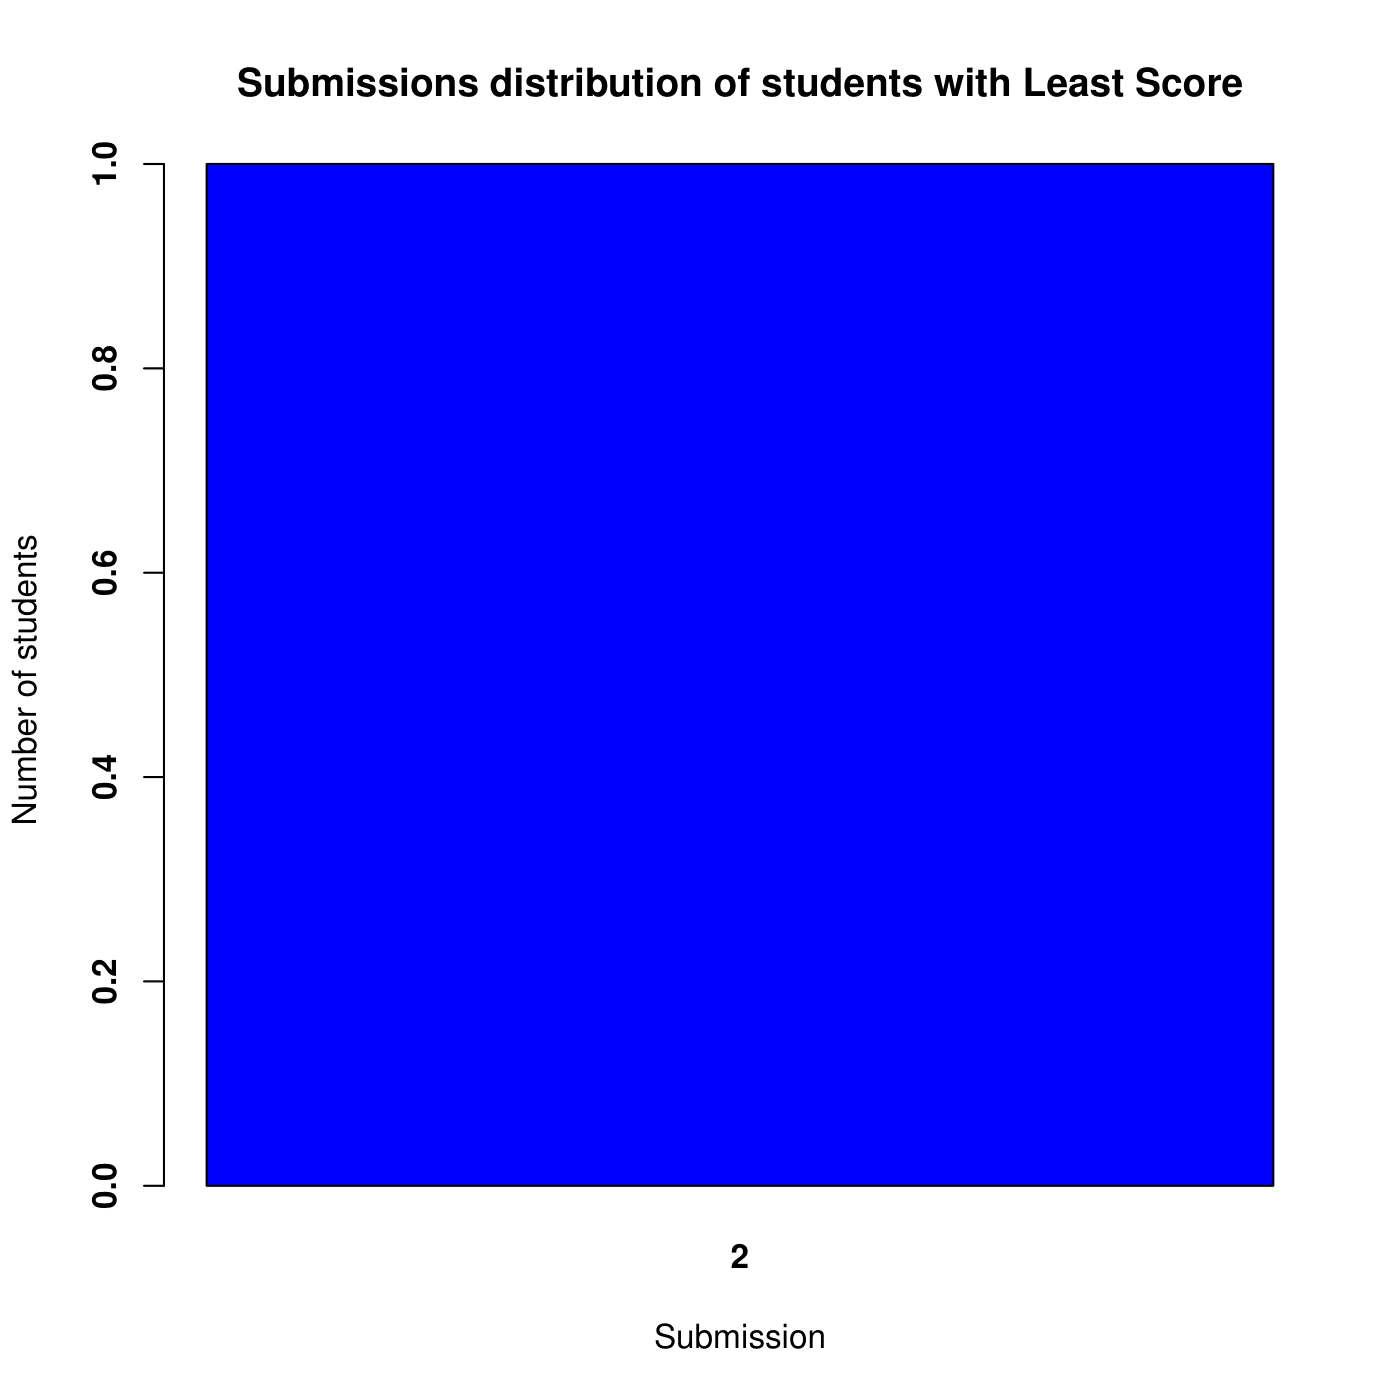
\includegraphics[width = 6.9cm]{Images/img2-1-1.png} & 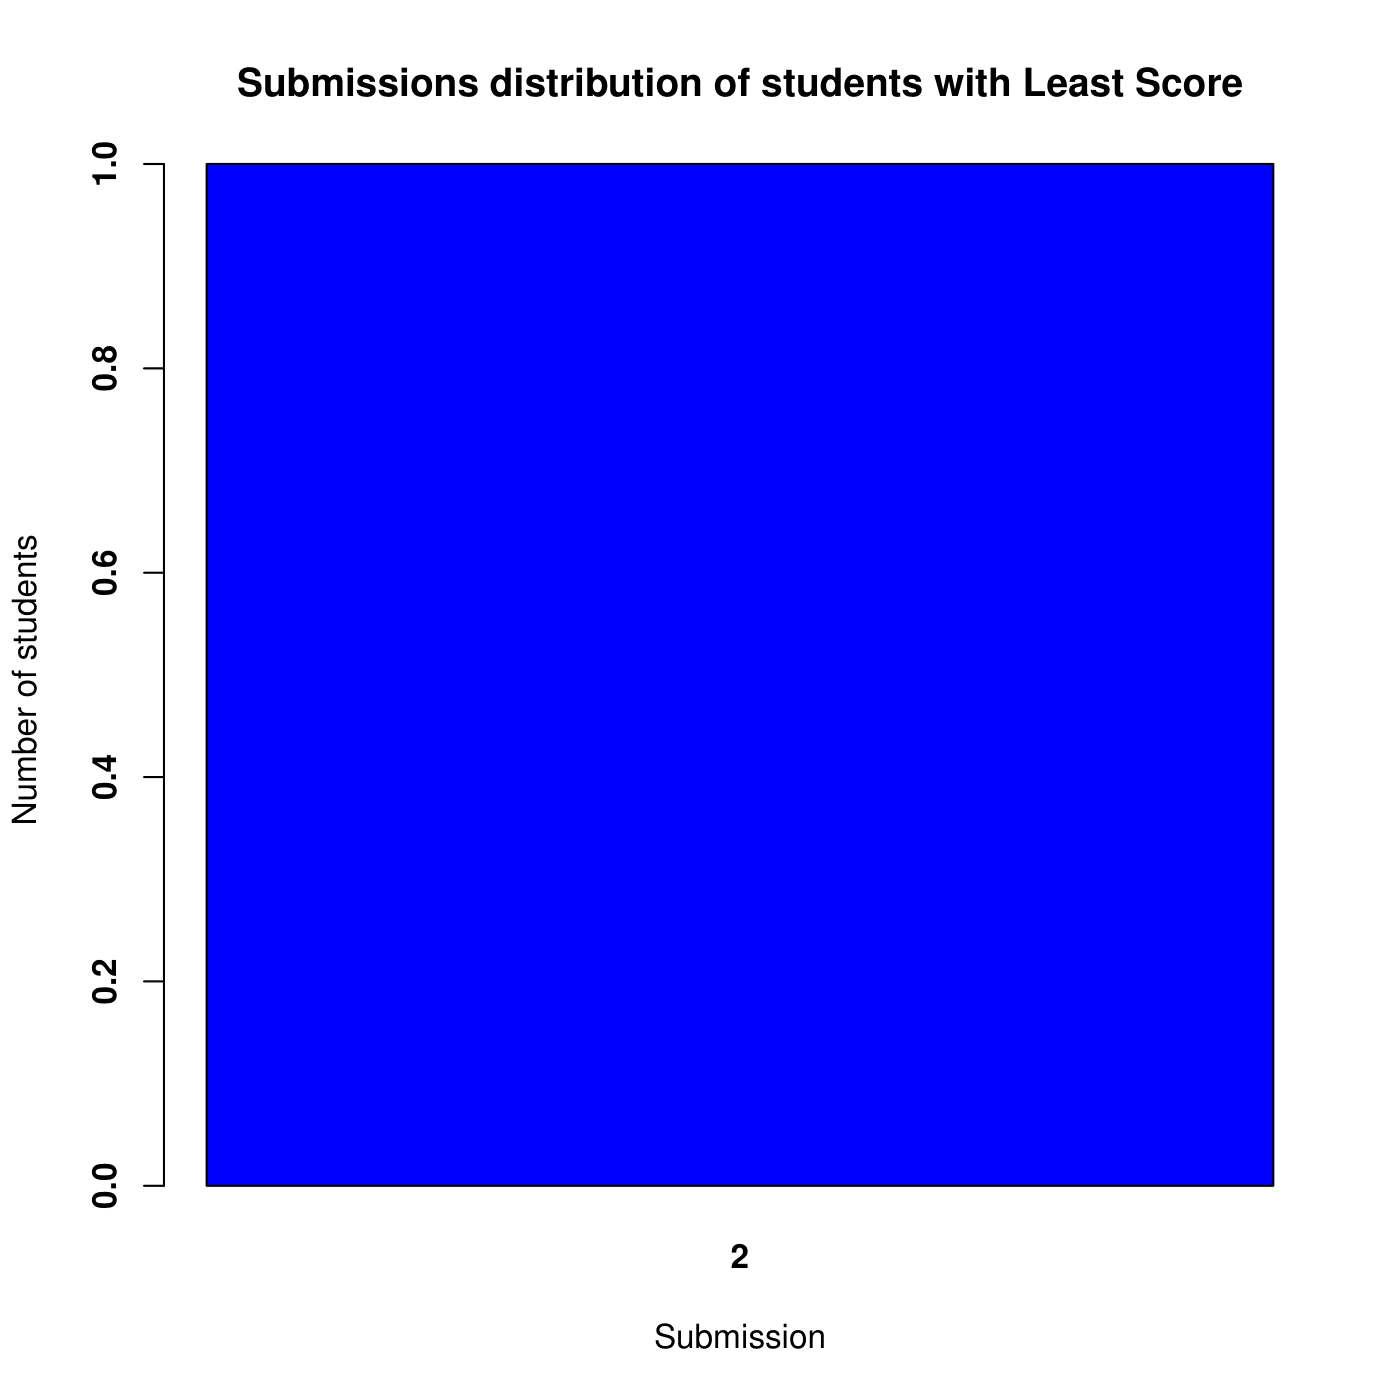
\includegraphics[width = 6.9cm]{Images/img2-1-2.png} \\
                 (1) & (2) \\
                 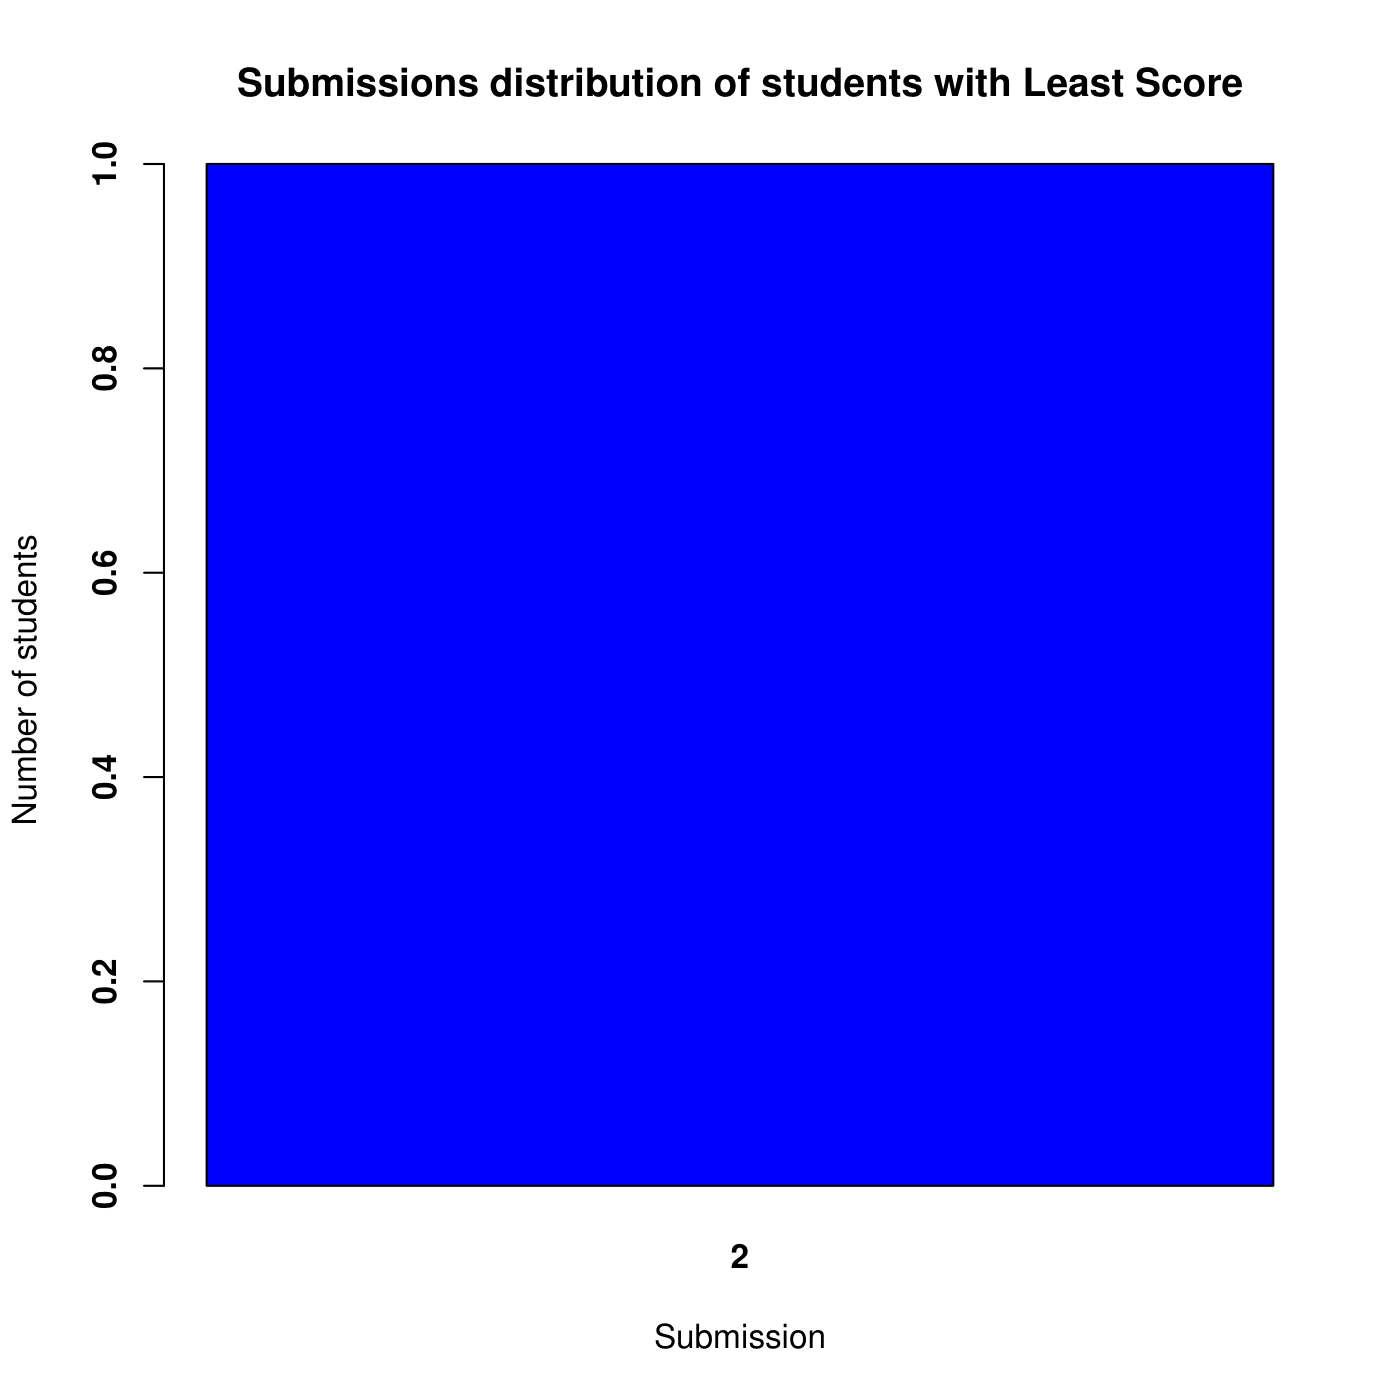
\includegraphics[width = 6.9cm]{Images/img2-1-3.png} &
                 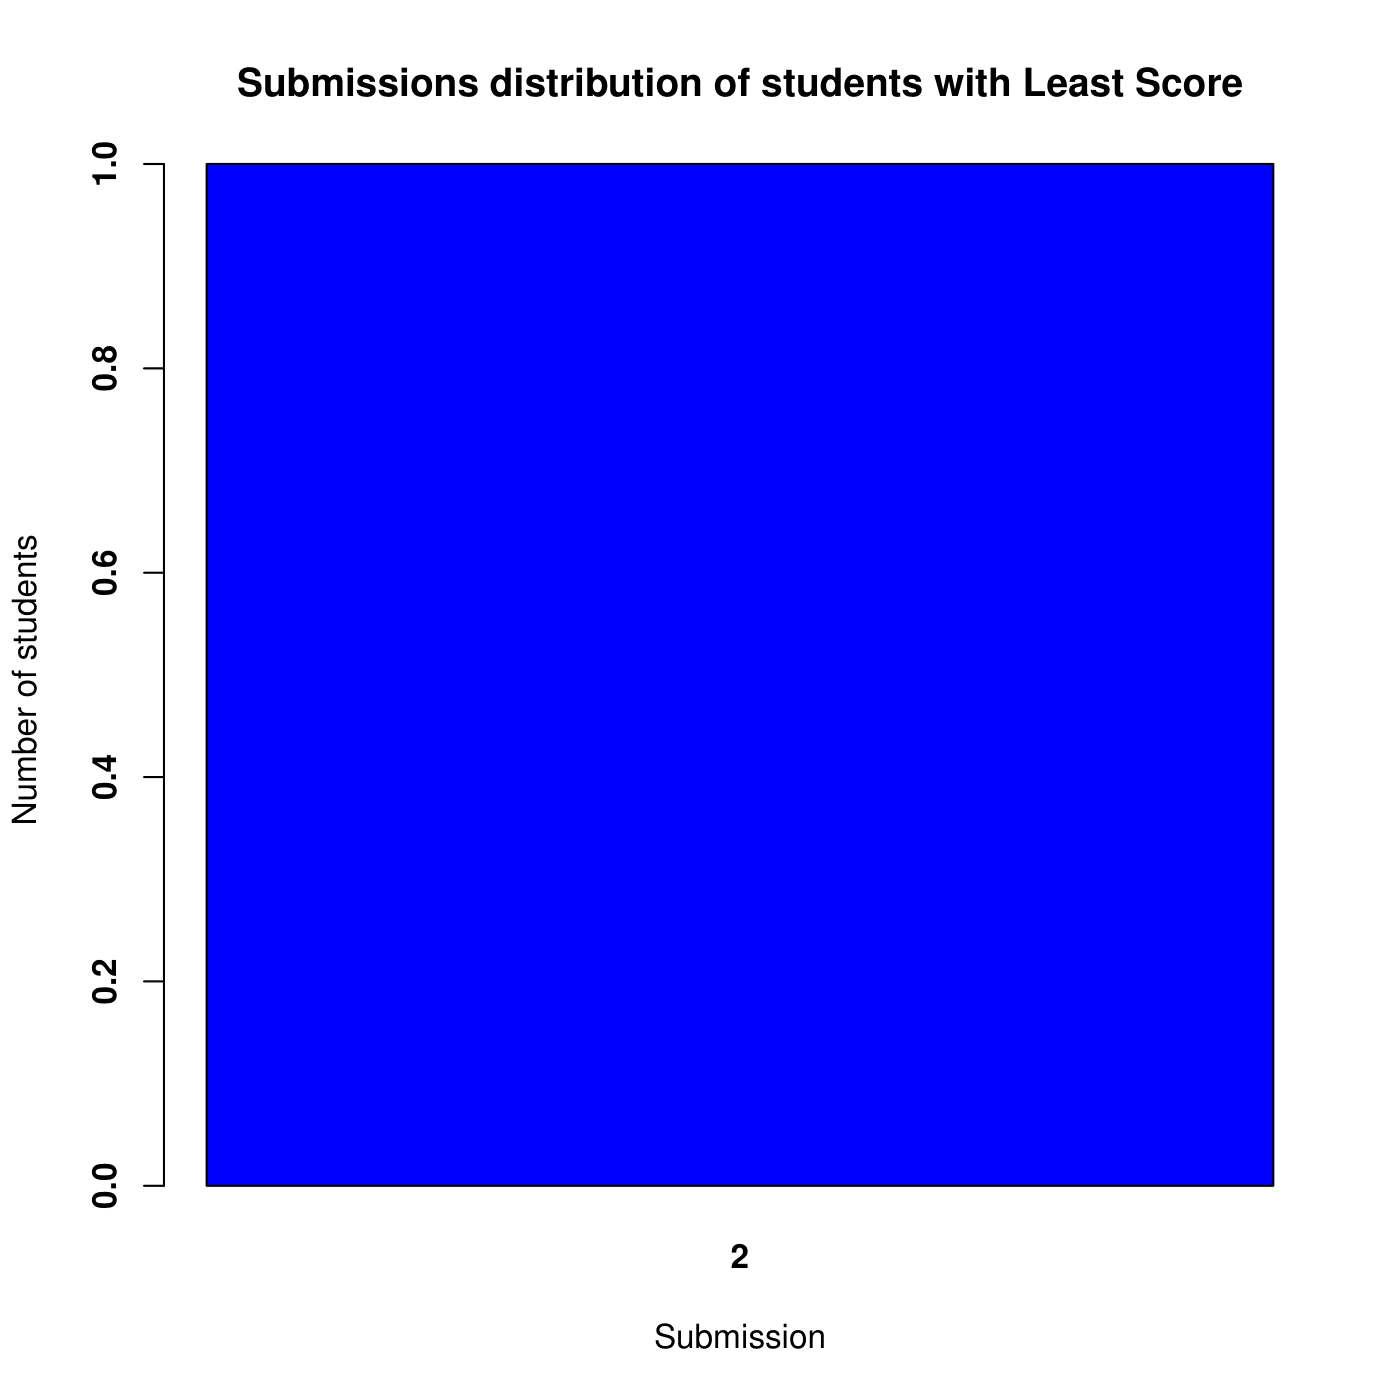
\includegraphics[width = 6.9cm]{Images/img2-1-4.png} \\
                 (3) & (4)
            \end{tabular}\\
            \textbf{Hình 2.1:} Phổ theo số lần nộp bài của các sinh viên có ít nhất một bài có số điểm thấp nhất\\
            \begin{tabular}{c c}
                 (1) & \texttt{"CO1007\_TV\_HK192-Quiz 1.4-điểm.xlsx"}\\
                 (2) & \texttt{"CO1007\_TV\_HK192-Quiz 1.5-điểm.xlsx"}\\
                 (3) & \texttt{"CO1007\_TV\_HK192-Quiz 3.3-điểm.xlsx"}\\
                 (4) & \texttt{"CO1007\_TV\_HK192-Quiz 4.2-điểm.xlsx"}
            \end{tabular}
        \end{center}
    \end{itemize}
    %Cau e
    \bf\item {Xác định điểm số tổng kết thấp nhất}\\[6pt]
    \bf Kiến thức chuẩn bị\normalfont
    \begin{itemize}
        \item Cách giải truyền thống:
        \begin{itemize}
            \item Ta lập danh sách các sinh viên với điểm số tổng kết của mỗi sinh viên, sau đó chọn ra số điểm tổng kết thấp nhất.
        \end{itemize}
    \end{itemize}
    \bf Hiện thực trên R\normalfont
    \begin{itemize}
        \item Ý tưởng thực hiện:
        \begin{itemize}
            \item Ta sắp xếp dữ liệu theo cột điểm từ cao đến thấp, và sử dụng hàm $match()$ và $unique()$ để giữ lại giá trị đầu tiên tính từ trên xuống (cũng là điểm tổng kết của các bạn).
            \item Bước đầu tạo một dataframe $K.Descend$ được sắp thứ tự từ cao đến thấp của dữ liệu ban đầu.
            \begin{center}
                \begin{tabular}{p{13cm}}
                    \texttt{K.Descend <- K[order(-K\$Total),]}
                \end{tabular}
            \end{center}
            \item Tạo tiếp một dataframe $K.Descend.Unique$ để lọc ra những lần làm bài có điểm cao nhất của mỗi bạn sinh viên từ $K.Descend$.
            \begin{center}
                \begin{tabular}{p{13cm}}
                    \texttt{K.Descend.Unique <- K.Descend[match(unique(K.Descend\$ID), K.Descend\$ID),]}
                \end{tabular}
            \end{center}
            Vậy điểm tổng kết nhỏ nhất sẽ là điểm có giá trị nhỏ nhất trong $K.Descend.Unique$.
            \begin{center}
                \begin{tabular}{p{13cm}}
                    \texttt{Least.Final.Total <- min(K.Desecend.Unique\$Total)}
                \end{tabular}
            \end{center}
        \end{itemize}
        \item Kết quả:
        \begin{itemize}
            \item Điểm số tổng kết thấp nhất của mỗi file:
            \begin{center}
                \begin{tabular}{l c}
                     \texttt{"CO1007\_TV\_HK192-Quiz 1.4-điểm.xlsx"} & 8 điểm\\
                     \texttt{"CO1007\_TV\_HK192-Quiz 1.5-điểm.xlsx"} & 7 điểm\\
                     \texttt{"CO1007\_TV\_HK192-Quiz 3.3-điểm.xlsx"} & 8 điểm\\
                     \texttt{"CO1007\_TV\_HK192-Quiz 4.2-điểm.xlsx"} & 7 điểm
                \end{tabular}
            \end{center}
        \end{itemize}
    \end{itemize}
    %Cau f
    \bf\item {Xác định danh sách các sinh viên có điểm số tổng kết thấp nhất}\\[6pt]
    \bf Kiến thức chuẩn bị\normalfont
    \begin{itemize}
        \item Cách giải truyền thống:
        \begin{itemize}
            \item Dựa vào điểm số tổng kết nhỏ nhất tính được ở câu $e$ và bảng dữ liệu, ta lập danh sách sinh viên có điểm tổng kết thấp nhất.
        \end{itemize}
    \end{itemize}
    \bf Hiện thực trên R\normalfont
    \begin{itemize}
        \item Ý tưởng thực hiện:
        \begin{itemize}
            \item Lưu ý rằng $K.Descend.Unique$ là danh sách điểm tổng kết của các bạn sinh viên.
            \begin{center}
                \begin{tabular}{p{13cm}}
                    \texttt{List.Of.Final.Total <- K.Descend.Unique}
                \end{tabular}
            \end{center}
            \item Vậy $List.Of.Final.Total$ là danh sách điểm tổng kết. Như vậy ta có thể tạo một subset là danh sách các bạn sinh viên từ dataframe $List.Of.Final.Total$ và điểm tổng kết thấp nhất ($Least.Final.Total$) từ câu trên.
            \begin{center}
                \begin{tabular}{p{13cm}}
                    \texttt{List.Least.Final.Total <- subset(List.Of.Final.Total, Total == Least.Final.Total)}
                \end{tabular}
            \end{center}
            \item $List.Least.Final.Total$ là danh sách các sinh viên có điểm số tổng kết thấp nhất cần tìm.
        \end{itemize}
        \item Kết quả:
        \begin{itemize}
            \item Danh sách sinh viên có điểm tổng kết thấp nhất của mỗi file:
            \begin{center}
                \begin{tabular}{l c c c c}
                     \texttt{"CO1007\_TV\_HK192-Quiz 1.4-điểm.xlsx"} & 1913334 & 1915928 & 1915275 & 1914661\\
                     \texttt{"CO1007\_TV\_HK192-Quiz 1.5-điểm.xlsx"} & 1812478 & 1812257 & 1915275 & 1914079\\
                     & 1911975\\
                     \texttt{"CO1007\_TV\_HK192-Quiz 3.3-điểm.xlsx"} & 1912523 & 1913218 & 1912966\\
                     \texttt{"CO1007\_TV\_HK192-Quiz 4.2-điểm.xlsx"} & 1914210
                \end{tabular}
            \end{center}
        \end{itemize}
    \end{itemize}
    %Cau g
    \bf\item {Xác định phổ theo số lần nộp bài của các sinh viên có điểm số tổng kết thấp nhất}\\[6pt]
    \bf Kiến thức chuẩn bị\normalfont
    \begin{itemize}
        \item Cách giải truyền thống:
        \begin{itemize}
            \item Từ danh sách tìm được ở câu $f$ và danh sách ban đầu tìm được số lần nộp bài của các sinh viên, ta vẽ phổ theo số lần nộp bài của các sinh viên có điểm số tổng kết thấp nhất.
        \end{itemize}
    \end{itemize}
    \bf Hiện thực trên R\normalfont
    \begin{itemize}
        \item Ý tưởng thực hiện:
        \begin{itemize}
            \item Ta sử dụng các hàm $subset()$ và $table()$ để lấy danh sách các lượt làm bài của các bạn có điểm tổng kết nhỏ nhất.
            \begin{center}
                \begin{tabular}{p{13cm}}
                    \texttt{List.Least.Final.Total2 <- subset(K, ID \%in\% List.Least.Final.Total\$ID)}
                \end{tabular}
            \end{center}
            \item $List.Least.Final.Total2$ là danh sách các lượt làm bài của các bạn có điểm tổng kết nhỏ nhất.
            \begin{center}
                \begin{tabular}{p{13cm}}
                    \texttt{List.Least.Final.Total.Freq <- data.frame(table(List.Least.Final.Total2\$ID))}
                \end{tabular}
            \end{center}
            \item $List.Least.Final.Total.Freq$ là danh sách số lần nộp bài của sinh viên có điểm số tổng kết thấp nhất. Ta dùng hàm $barplot()$ để vẽ phổ số lần nộp bài của nhóm sinh viên trên.
        \end{itemize}
        \item Biểu đồ:\\
        \begin{center}
            \begin{tabular}{c c}
                 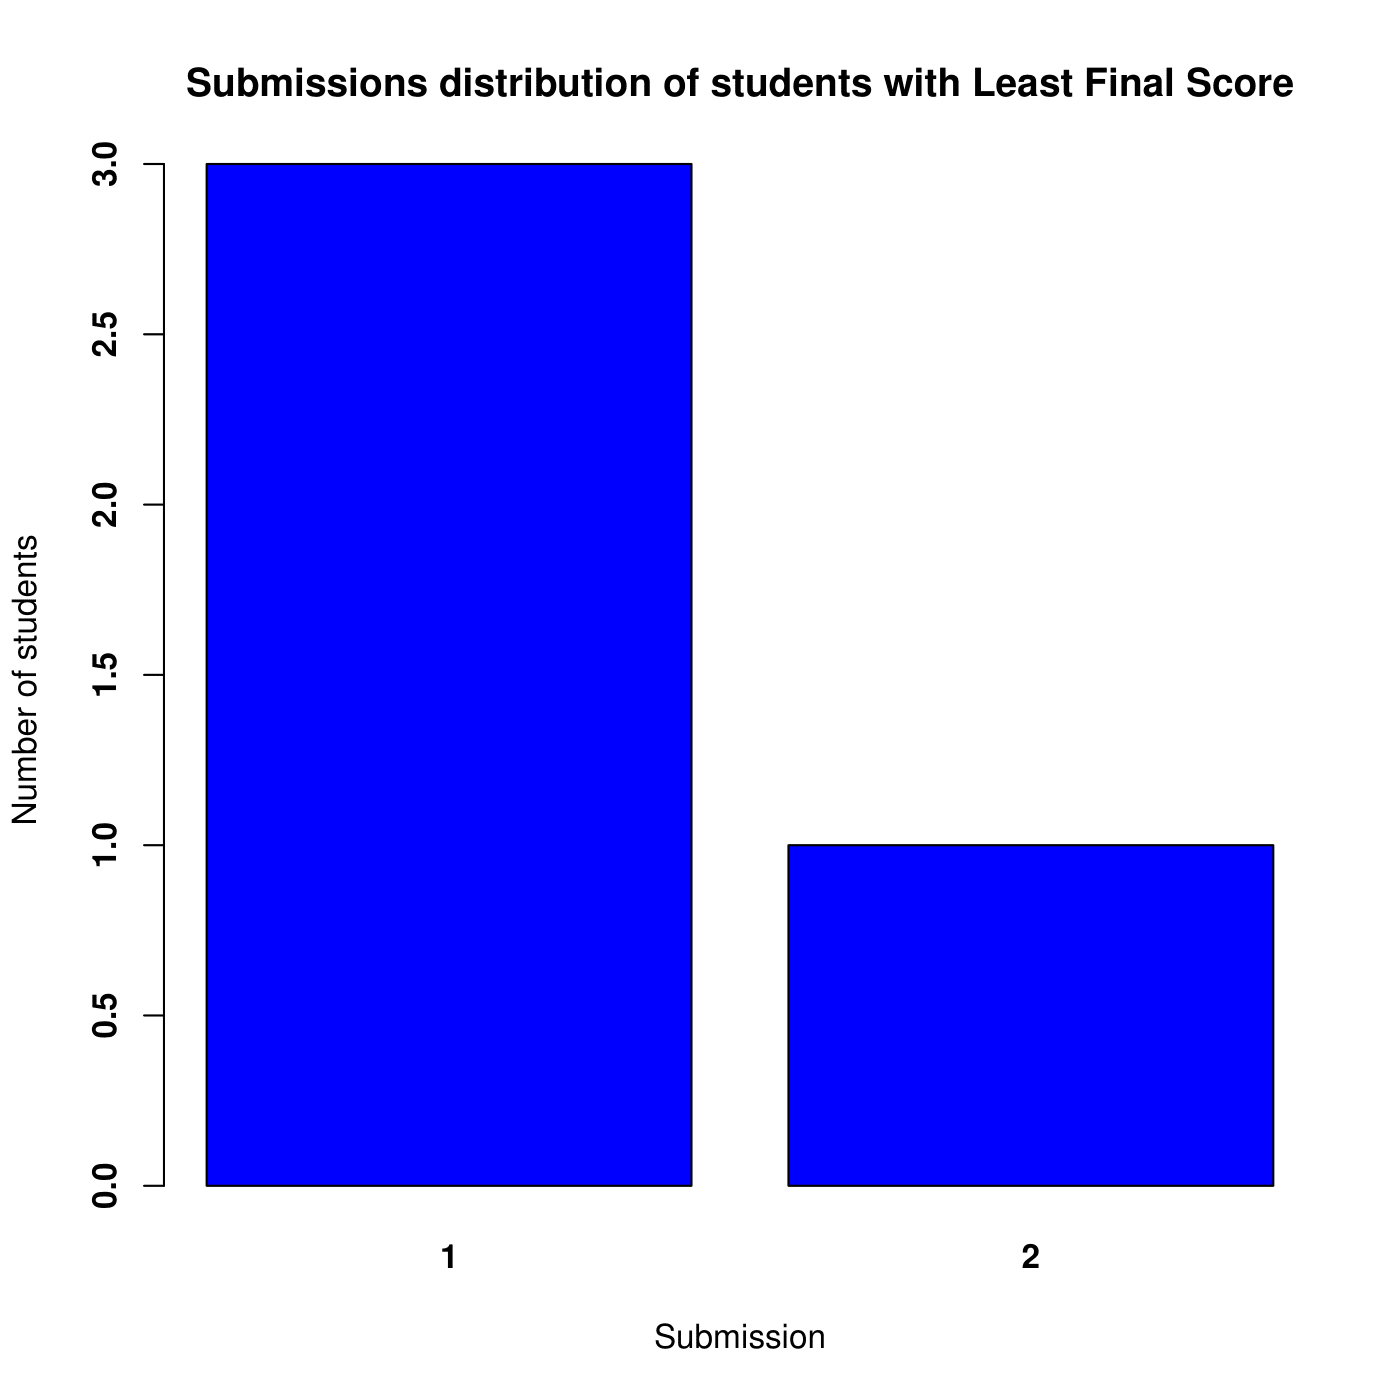
\includegraphics[width = 6.9cm]{Images/img2-2-1.png} & 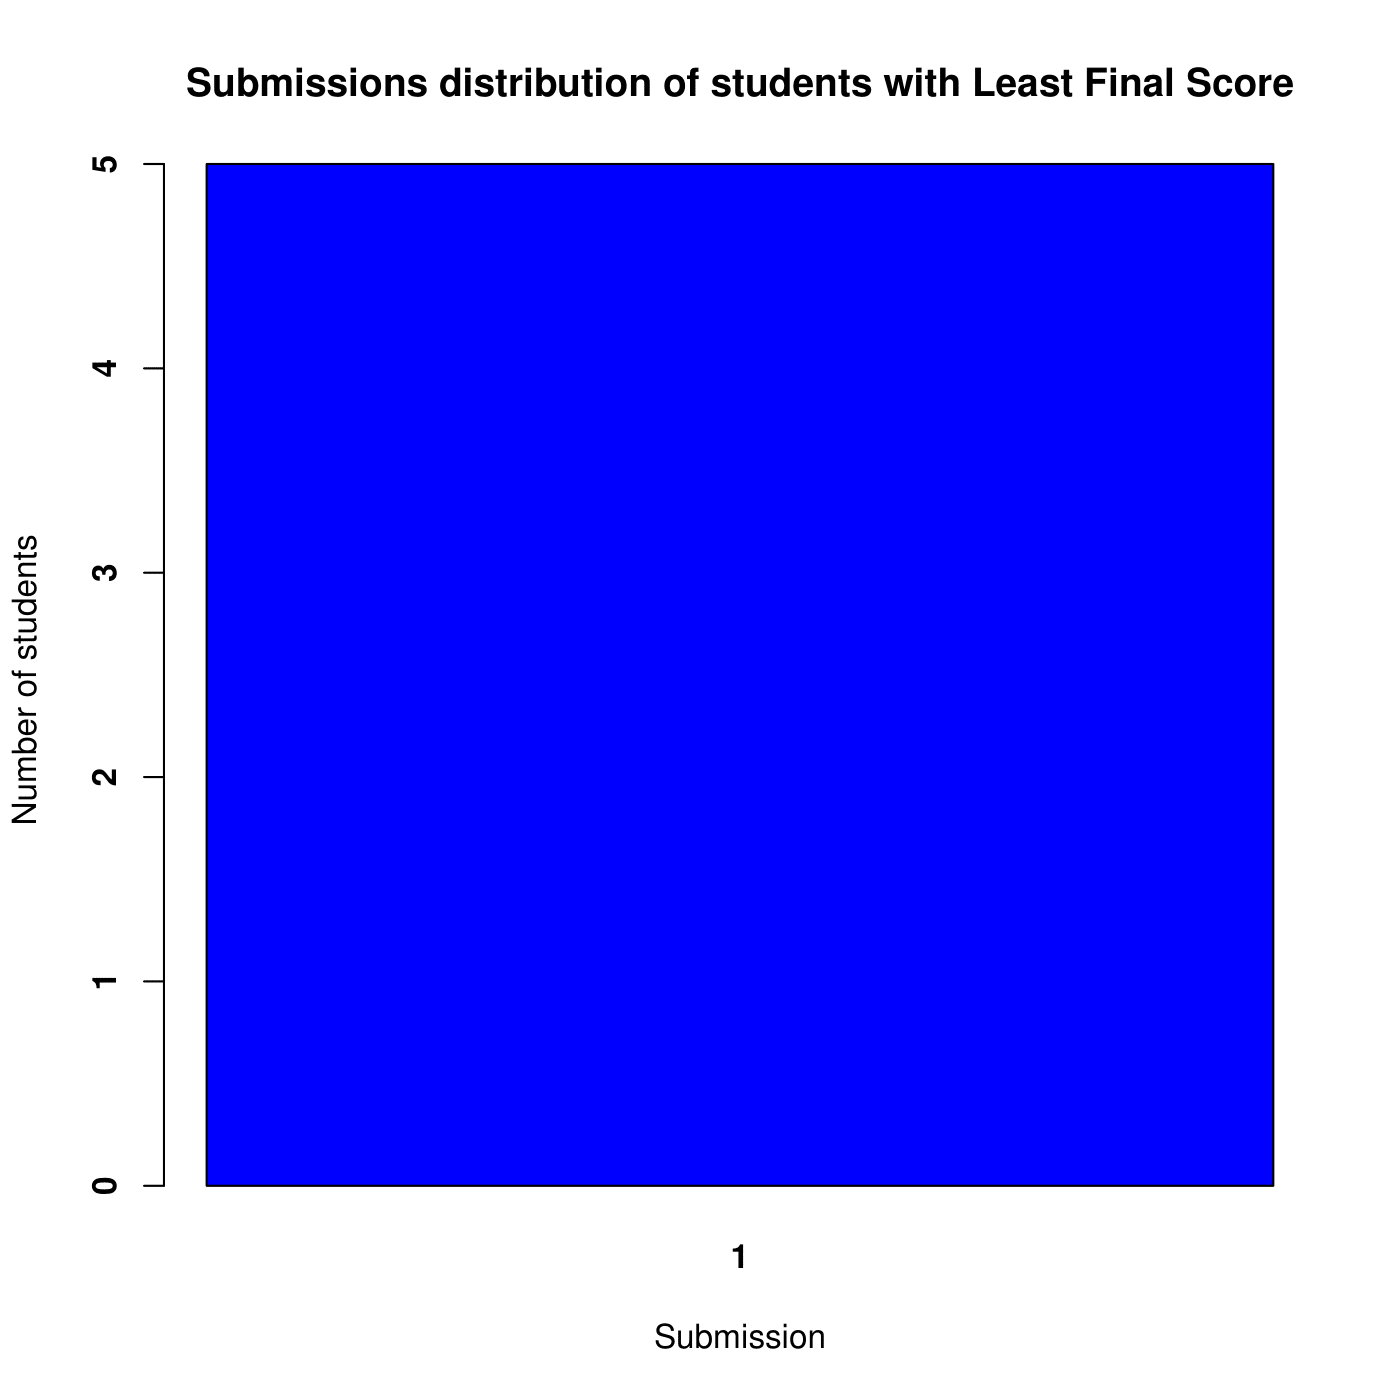
\includegraphics[width = 6.9cm]{Images/img2-2-2.png} \\
                 (1) & (2) \\
                 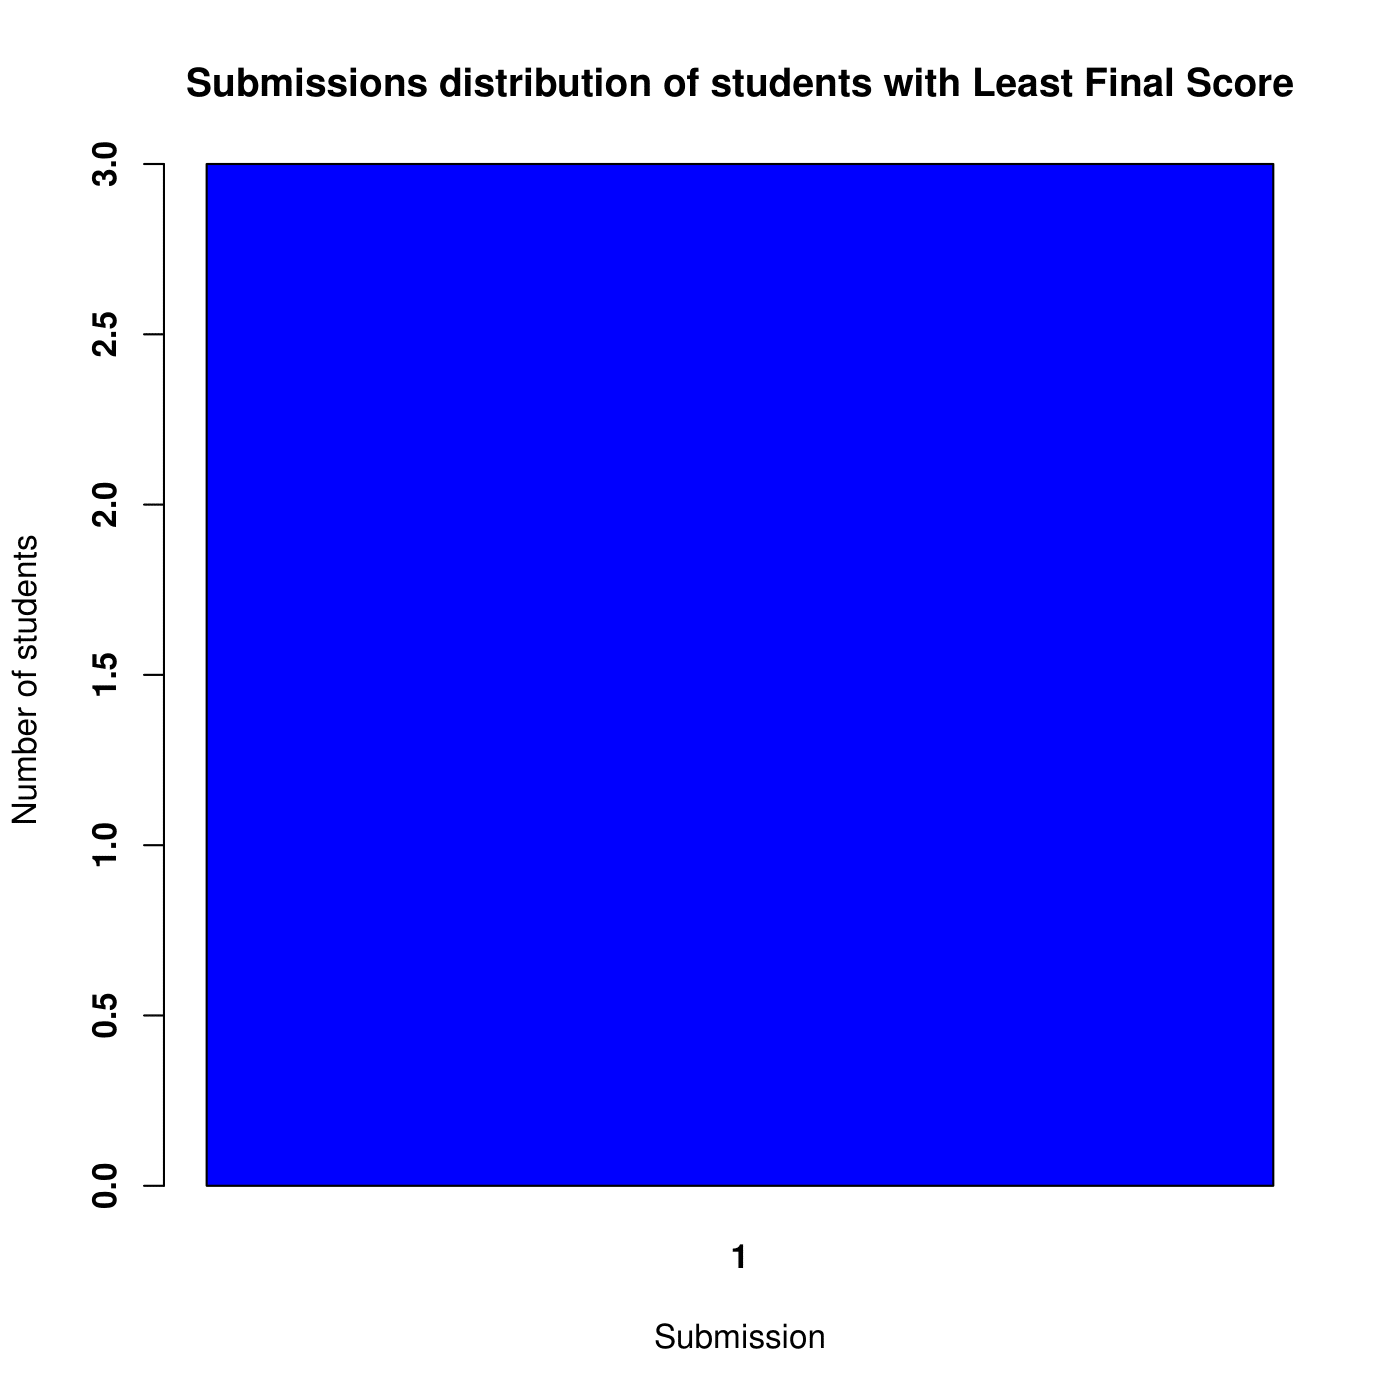
\includegraphics[width = 6.9cm]{Images/img2-2-3.png} &
                 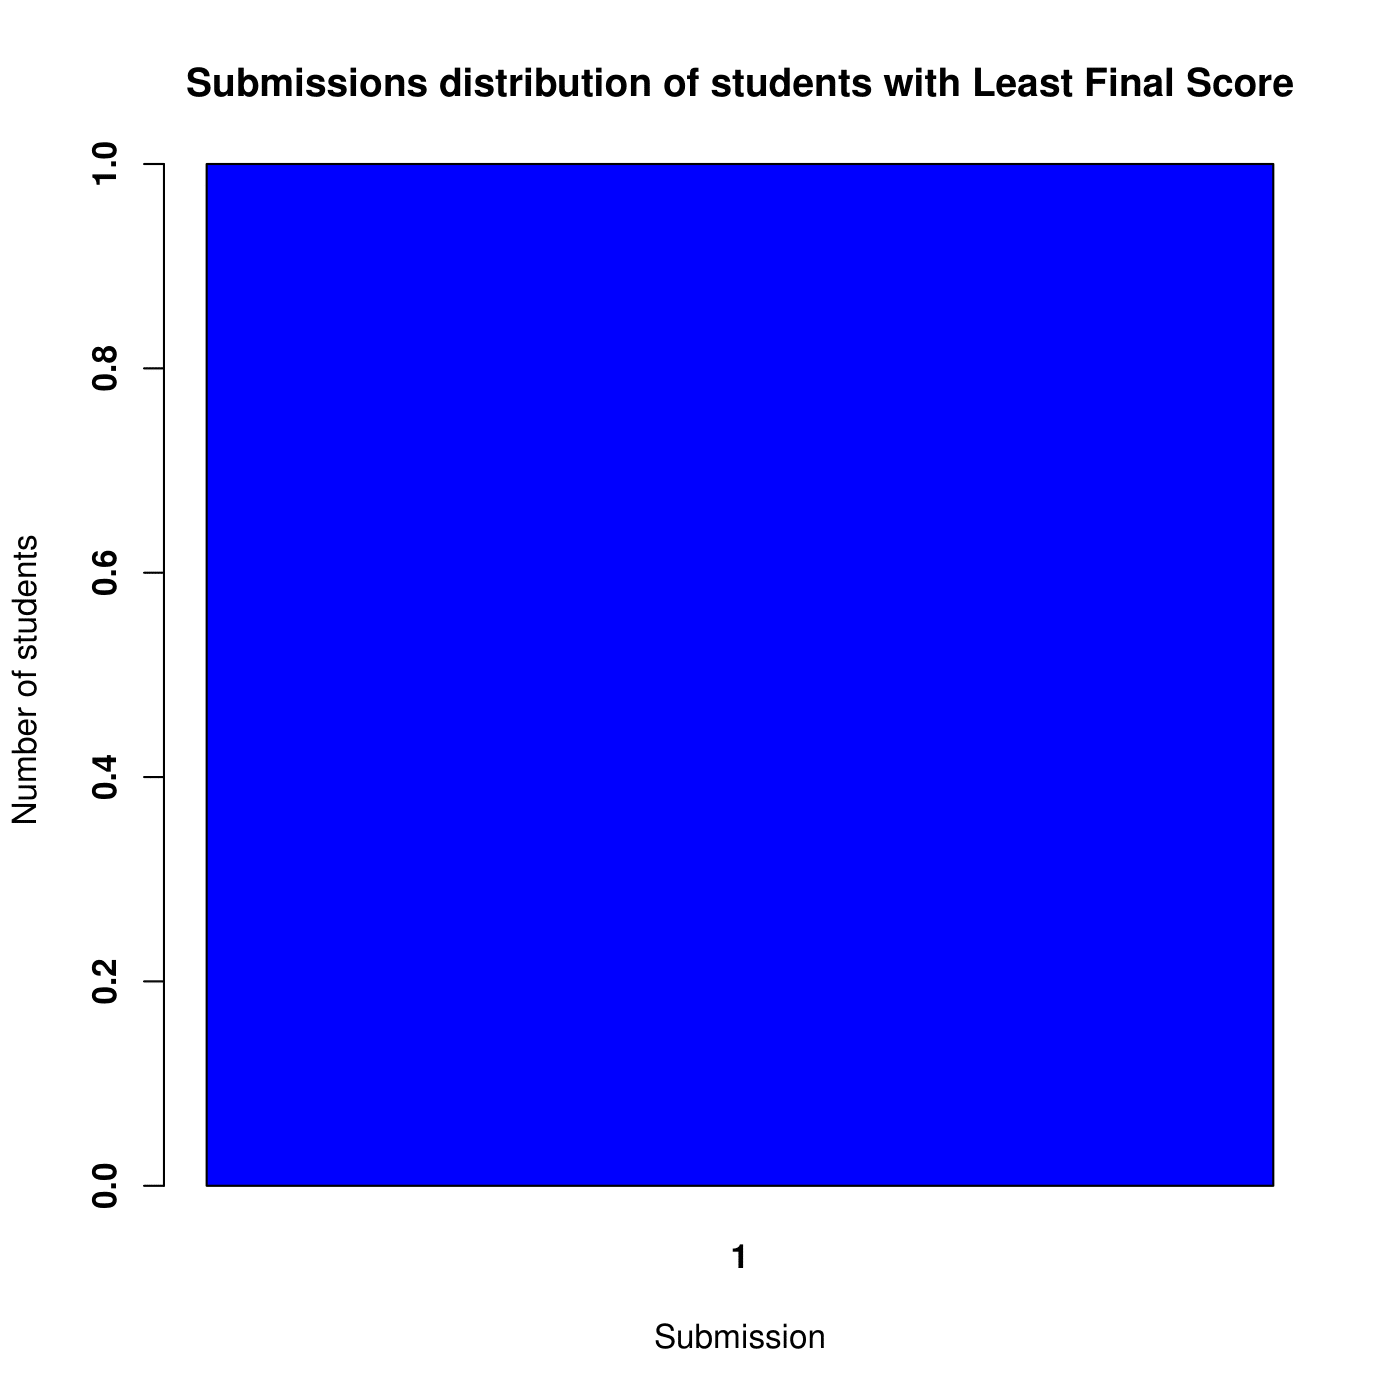
\includegraphics[width = 6.9cm]{Images/img2-2-4.png} \\
                 (3) & (4)
            \end{tabular}\\
            \textbf{Hình 2.2:} Phổ theo số lần nộp bài của các sinh viên có điểm số tổng kết thấp nhất\\
            \begin{tabular}{c c}
                 (1) & \texttt{"CO1007\_TV\_HK192-Quiz 1.4-điểm.xlsx"}\\
                 (2) & \texttt{"CO1007\_TV\_HK192-Quiz 1.5-điểm.xlsx"}\\
                 (3) & \texttt{"CO1007\_TV\_HK192-Quiz 3.3-điểm.xlsx"}\\
                 (4) & \texttt{"CO1007\_TV\_HK192-Quiz 4.2-điểm.xlsx"}
            \end{tabular}
        \end{center}
    \end{itemize}
    %Cau h
    \bf\item {Xác định điểm số cao nhất}\\[6pt]
    \bf Kiến thức chuẩn bị\normalfont
    \begin{itemize}
        \item Cách giải truyền thống:
        \begin{itemize}
            \item Dựa vào danh sách dữ liệu điểm, ta tìm được điểm số cao nhất.
        \end{itemize}
    \end{itemize}
    \bf Hiện thực trên R\normalfont
    \begin{itemize}
        \item Ý tưởng thực hiện:
        \begin{itemize}
            \item Ta dùng hàm $max()$ để tìm giá trị lớn nhất của một vector.
            \begin{center}
                \begin{tabular}{p{13cm}}
                    \texttt{Highest.Total <- max(K[,6])}
                \end{tabular}
            \end{center}
        \end{itemize}
        \item Kết quả:
        \begin{itemize}
            \item Điểm số cao nhất của mỗi file:
            \begin{center}
                \begin{tabular}{l c}
                     \texttt{"CO1007\_TV\_HK192-Quiz 1.4-điểm.xlsx"} & 10 điểm\\
                     \texttt{"CO1007\_TV\_HK192-Quiz 1.5-điểm.xlsx"} & 10 điểm\\
                     \texttt{"CO1007\_TV\_HK192-Quiz 3.3-điểm.xlsx"} & 10 điêm\\
                     \texttt{"CO1007\_TV\_HK192-Quiz 4.2-điểm.xlsx"} & 10 điểm
                \end{tabular}
            \end{center}
        \end{itemize}
    \end{itemize}
    %Cau i
    \bf\item {Xác định danh sách các sinh viên có tối thiểu một bài nộp có số điểm số cao nhất}\\[6pt]
    \bf Kiến thức chuẩn bị\normalfont
    \begin{itemize}
        \item Cách giải truyền thống:
        \begin{itemize}
            \item Dựa vào giá trị tìm được ở câu $h$, ta lập danh sách những sinh viến có ít nhất một bài nộp có số điểm cao nhất.
        \end{itemize}
    \end{itemize}
    \bf Hiện thực trên R\normalfont
    \begin{itemize}
        \item Ý tưởng thực hiện:
        \begin{itemize}
            \item Ta sử dụng hàm $subset()$ để lọc ra các danh sách các bài nộp có điểm số bằng số điểm cao nhất. Sau đó, ta sử dụng hàm $unique()$ để lấy danh sách sinh viên từ dữ liệu vừa lọc ra được.
            \begin{center}
                \begin{tabular}{p{13cm}}
                    \texttt{List.Highest.Total <- subset(K, K\$Total == Highest.Total)}\\
                    \texttt{List.Highest.Total.Unique <- List.Highest.Total[match(unique( List.Highest.Total\$ID), List.Highest.Total\$ID), ]}
                \end{tabular}
            \end{center}
        \end{itemize}
        \item Kết quả:
        \begin{itemize}
            \item Danh sách các sinh viên có ít nhất một bài có điểm số cao nhất của mỗi file:
            \begin{center}
                \begin{tabular}{l c c c c}
                     \texttt{"CO1007\_TV\_HK192-Quiz 1.4-điểm.xlsx"} & 1915562 & 1913355 & 1914038 & 1913464\\
                     & 1913186 & 1915919 & 1912041 & 1911591\\
                     & 1910916 & 1914845 & 1915329 & 1911704\\
                     & 1910666 & 1910351 & 1913467 & 1915323\\
                     & 1914055 & 1915268 & 1914864 & 1910032\\
                     & ...\\
                     \texttt{"CO1007\_TV\_HK192-Quiz 1.5-điểm.xlsx"} & 1913094 & 1914807 & 1914352 & 1913844 \\
                     & 1913464 & 1915323 & 1911478 & 1913186\\
                     & 1915822 & 1913014 & 1937019 & 1911591\\
                     & 1911704 & 1914845 & 1913336 & 1910202\\
                     & 1913355 & 1915540 & 1911186 & 1910101\\
                     & ...\\
                     \texttt{"CO1007\_TV\_HK192-Quiz 3.3-điểm.xlsx"} & 1914720 & 1911591 & 1913566 & 1912817\\
                     & 1915482 & 1913775 & 1913355 & 1915329\\
                     & 1911704 & 1910666 & 1913186 & 1914845\\
                     & 1915541 & 1914474 & 1911136 & 1915473\\
                     & 1911837 & 1912980 & 1914003 & 1911881\\
                     & ...\\
                     \texttt{"CO1007\_TV\_HK192-Quiz 4.2-điểm.xlsx"} & 1911881 & 1913355 & 1913186 & 1913014\\
                     & 1915482 & 1910666 & 1911591 & 1911704\\
                     & 1913241 & 1911314 & 1914845 & 1913123\\
                     & 1914003 & 1911136 & 1913075 & 1912817\\
                     & 1915541 & 1914720 & 1912811 & 1913396\\
                     & ...
                \end{tabular}
            \end{center}
        \end{itemize}
    \end{itemize}
    %Cau j
    \bf\item {Xác định phổ theo số lần nộp bài của các sinh viên có tối thiểu một bài nộp có điểm số cao nhất}\\[6pt]
    \bf Kiến thức chuẩn bị\normalfont
    \begin{itemize}
        \item Cách giải truyền thống:
        \begin{itemize}
            \item Từ danh sách các bạn sinh viên có ít nhất một bài có số điểm cao nhất và danh sách ban đầu, ta tạo được một danh sách mới với các bạn sinh viên có ít nhất một bài có điểm số cao thấp và số lần làm bài của mỗi sinh viên, sau đó vẽ phổ theo số lần làm bài dựa trên tập dữ liệu vừa thu được.
        \end{itemize}
    \end{itemize}
    \bf Hiện thực trên R\normalfont
    \begin{itemize}
        \item Ý tưởng thực hiện:
        \begin{itemize}
            \item Ta sử dụng hàm $subset()$ để lọc ra từ tập giá trị ban đầu những sinh viên có ít nhất một bài đạt điểm cao nhất, sau đó sử dụng $table()$ để lập danh sách số lần nộp bài của mỗi bạn.
            \begin{center}
                \begin{tabular}{p{13cm}}
                    \texttt{List.Highest.Total2 <-subset(K, ID \%in\% List.Highest.Total.Unique\$ID)}\\
                    \texttt{List.Highest.Total.Freq <- data.frame(table(List.Highest.Total2\$ID))}
                \end{tabular}
            \end{center}
            \item Cuối cùng, ta sử dụng hàm $barplot()$ để vẽ phổ theo số lần nộp bài của nhóm sinh viên trên.
        \end{itemize}
        \item Biểu đồ:\\
        \begin{center}
            \begin{tabular}{c c}
                 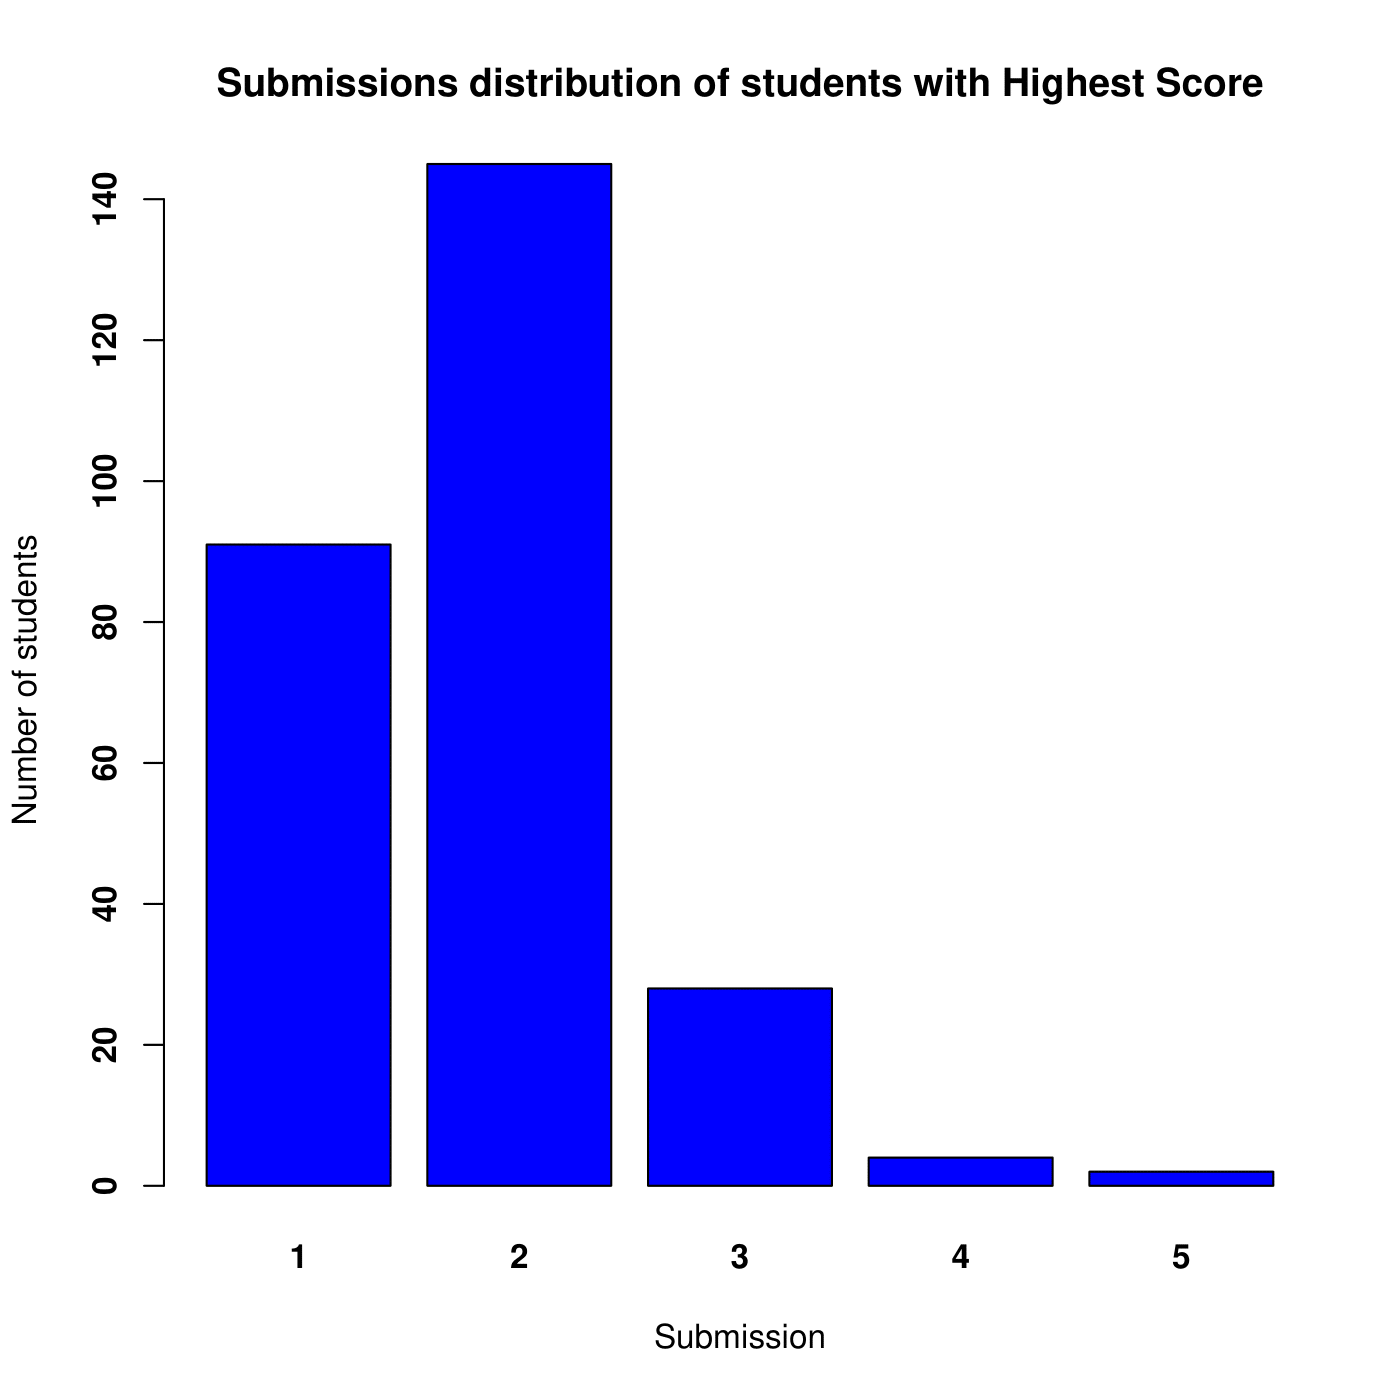
\includegraphics[width = 6.9cm]{Images/img2-3-1.png} & 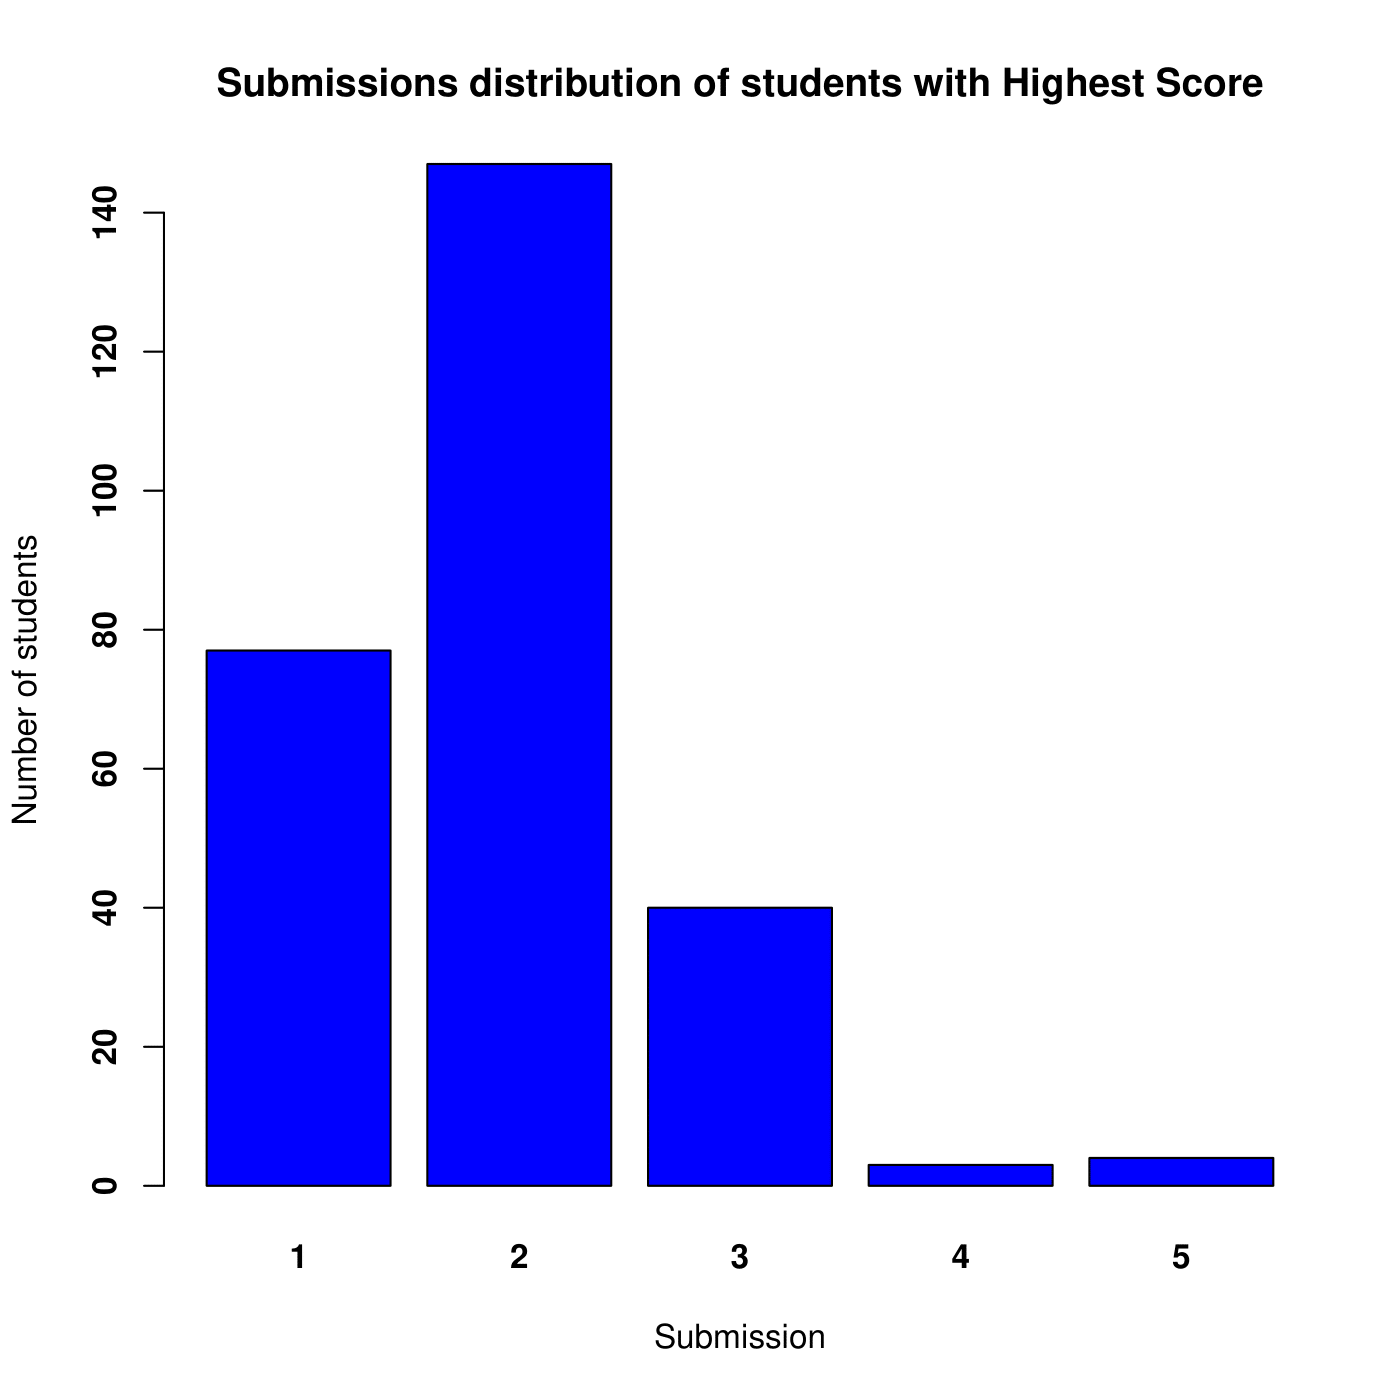
\includegraphics[width = 6.9cm]{Images/img2-3-2.png} \\
                 (1) & (2) \\
                 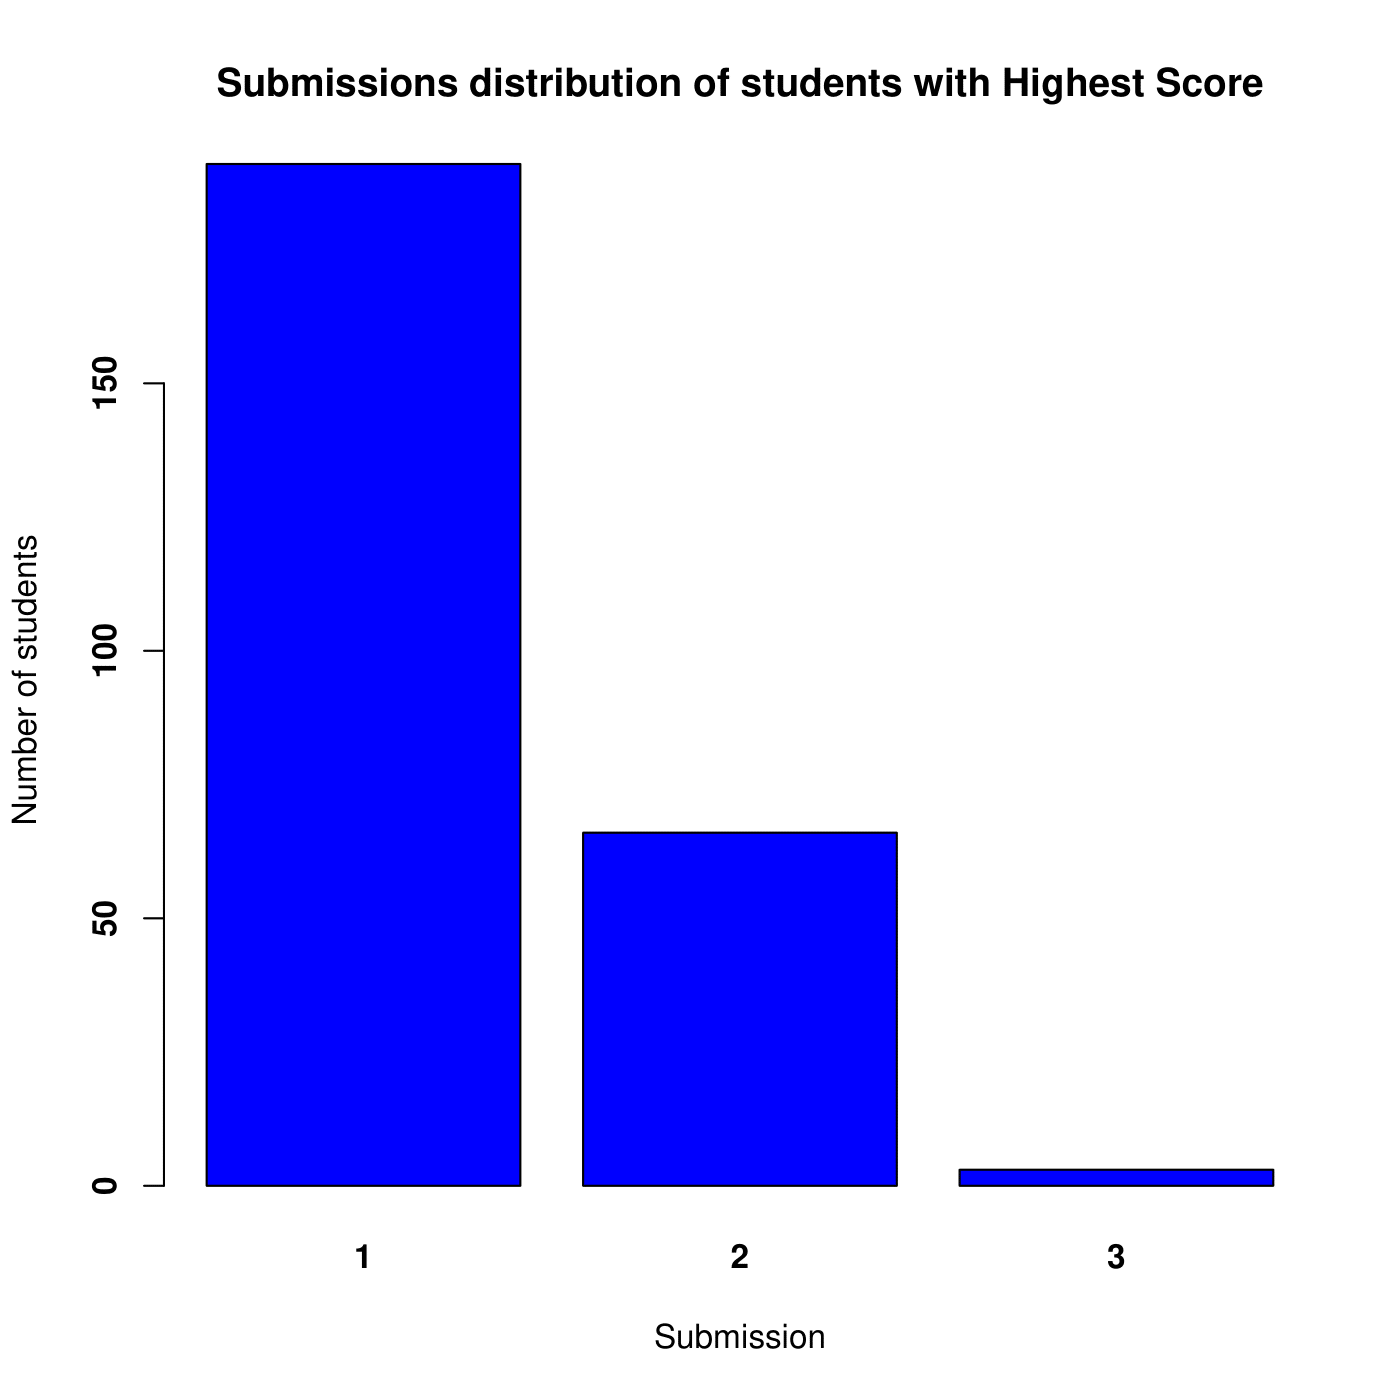
\includegraphics[width = 6.9cm]{Images/img2-3-3.png} &
                 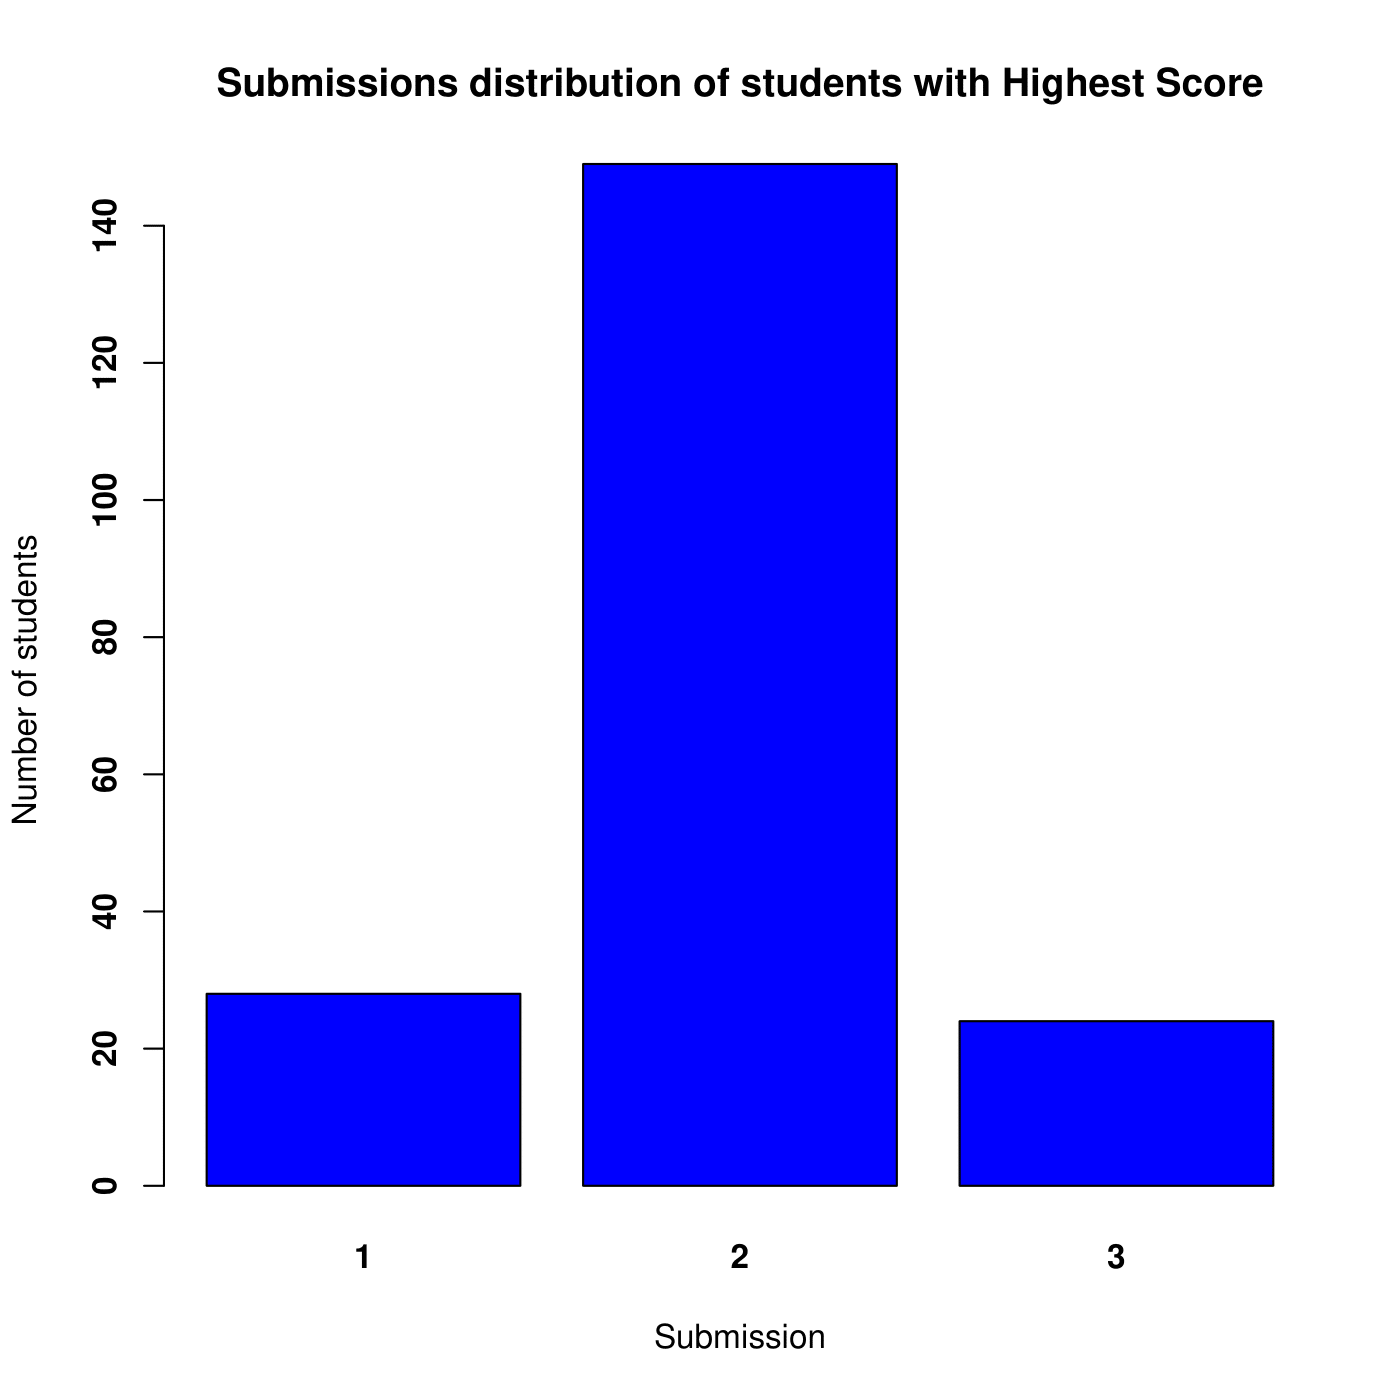
\includegraphics[width = 6.9cm]{Images/img2-3-4.png} \\
                 (3) & (4)
            \end{tabular}\\
            \textbf{Hình 2.3:} Phổ theo số lần nộp bài của các sinh viên có ít nhất một bài có số điểm cao nhất\\
            \begin{tabular}{c c}
                 (1) & \texttt{"CO1007\_TV\_HK192-Quiz 1.4-điểm.xlsx"}\\
                 (2) & \texttt{"CO1007\_TV\_HK192-Quiz 1.5-điểm.xlsx"}\\
                 (3) & \texttt{"CO1007\_TV\_HK192-Quiz 3.3-điểm.xlsx"}\\
                 (4) & \texttt{"CO1007\_TV\_HK192-Quiz 4.2-điểm.xlsx"}
            \end{tabular}
        \end{center}
    \end{itemize}
    %Cau k
    \bf\item {Xác định điểm số tổng kết cao nhất}\\[6pt]
    \bf Kiến thức chuẩn bị\normalfont
    \begin{itemize}
        \item Cách giải truyền thống:
        \begin{itemize}
            \item Ta lập danh sách điểm tổng kết của từng sinh viên, sau đó chọn ra điểm tổng kết coa nhất.
        \end{itemize}
    \end{itemize}
    \bf Hiện thực trên R\normalfont
    \begin{itemize}
        \item Ý tưởng thực hiện:
        \begin{itemize}
            \item Điểm tổng kết lớn nhất sẽ là điểm có giá trị lớn nhất trong $List.Of.Final.Total$ đã được tính ở câu $f$.
            \begin{center}
                \begin{tabular}{p{13cm}}
                    \texttt{Highest.Final.Total <- max(List.Of.Final.Total\$Total)}
                \end{tabular}
            \end{center}
        \end{itemize}
        \item Kết quả:
        \begin{itemize}
            \item Điểm số tổng kết cao nhất của mỗi file:
            \begin{center}
                \begin{tabular}{l c}
                     \texttt{"CO1007\_TV\_HK192-Quiz 1.4-điểm.xlsx"} & 10 điểm\\
                     \texttt{"CO1007\_TV\_HK192-Quiz 1.5-điểm.xlsx"} & 10 điểm\\
                     \texttt{"CO1007\_TV\_HK192-Quiz 3.3-điểm.xlsx"} & 10 điểm\\
                     \texttt{"CO1007\_TV\_HK192-Quiz 4.2-điểm.xlsx"} & 10 điểm
                \end{tabular}
            \end{center}
        \end{itemize}
    \end{itemize}
    %Cau l
    \bf\item {Xác định danh sách các sinh viên có điểm số tổng kết cao nhất}\\[6pt]
    \bf Kiến thức chuẩn bị\normalfont
    \begin{itemize}
        \item Cách giải truyền thống:
        \begin{itemize}
            \item Dựa vào điểm tổng kết cao nhất đã được xác định, ta lập danh sách những sinh viên có điểm tổng kết bằng điểm tổng két cao nhất.
        \end{itemize}
    \end{itemize}
    \bf Hiện thực trên R\normalfont
    \begin{itemize}
        \item Ý tưởng thực hiện:
        \begin{itemize}
            \item Ta tạo một subset là danh sách các bạn sinh viên từ dataframe $List.Of.Final.Total$ và điểm tổng kết cao nhất ($Highest.Final.Total$) từ câu $k$.
            \begin{center}
                \begin{tabular}{p{13cm}}
                    \texttt{List.Highest.Final.Total <- subset(List.Of.Final.Total, Total == Highest.Final.Total)}
                \end{tabular}
            \end{center}
            \item $List.Highest.Final.Total$ là danh sách các sinh viên có điểm số tổng kết cao nhất cần tìm.
        \end{itemize}
        \item Kết quả:
        \begin{itemize}
            \item Danh sách các sinh viên có điểm số tổng kết cao nhất của mỗi file:
            \begin{center}
                \begin{tabular}{l c c c c}
                     \texttt{"CO1007\_TV\_HK192-Quiz 1.4-điểm.xlsx"} & 1915562 & 1913355 & 1914038 & 1913464\\
                     & 1913186 & 1915919 & 1912041 & 1911591\\
                     & 1910916 & 1914845 & 1915329 & 1911704\\
                     & 1910666 & 1910351 & 1913467 & 1915323\\
                     & 1914055 & 1915268 & 1914864 & 1910032\\
                     & ...\\
                     \texttt{"CO1007\_TV\_HK192-Quiz 1.5-điểm.xlsx"} & 1913094 & 1914807 & 1914352 & 1913844 \\
                     & 1913464 & 1915323 & 1911478 & 1913186\\
                     & 1915822 & 1913014 & 1937019 & 1911591\\
                     & 1911704 & 1914845 & 1913336 & 1910202\\
                     & 1913355 & 1915540 & 1911186 & 1910101\\
                     & ...\\
                     \texttt{"CO1007\_TV\_HK192-Quiz 3.3-điểm.xlsx"} & 1914720 & 1911591 & 1913566 & 1912817\\
                     & 1915482 & 1913775 & 1913355 & 1915329\\
                     & 1911704 & 1910666 & 1913186 & 1914845\\
                     & 1915541 & 1914474 & 1911136 & 1915473\\
                     & 1911837 & 1912980 & 1914003 & 1911881\\
                     & ...\\
                     \texttt{"CO1007\_TV\_HK192-Quiz 4.2-điểm.xlsx"} & 1911881 & 1913355 & 1913186 & 1913014\\
                     & 1915482 & 1910666 & 1911591 & 1911704\\
                     & 1913241 & 1911314 & 1914845 & 1913123\\
                     & 1914003 & 1911136 & 1913075 & 1912817\\
                     & 1915541 & 1914720 & 1912811 & 1913396\\
                     & ...
                \end{tabular}
            \end{center}
        \end{itemize}
    \end{itemize}
    %Cau m
    \bf\item {Xác định phổ theo số lần nộp bài của các sinh viên có điểm số tổng kết cao nhất}\\[6pt]
    \bf Kiến thức chuẩn bị\normalfont
    \begin{itemize}
        \item Cách giải truyền thống:
        \begin{itemize}
            \item Từ danh sách các sinh viên tìm được ở câu $l$ và danh sách ban đầu, ta tìm được số lần nộp bài của các sinh viên theo yêu cầu bài toán. Sau đó, ta vẽ phổ theo số lần nộp bài của các sinh viên có điểm số tổng kết cao nhất.
        \end{itemize}
    \end{itemize}
    \bf Hiện thực trên R\normalfont
    \begin{itemize}
        \item Ý tưởng thực hiện:
        \begin{itemize}
            \item Ta sử dụng các hàm $subset()$ và $table()$ để lập danh sách số lần nộp bài của sinh viên có điểm số tổng kết cao nhất.
            \begin{center}
                \begin{tabular}{p{13cm}}
                    \texttt{List.Highest.Final.Total2 <-subset(K, ID \%in\% List.Highest.Final.Total\$ID)}
                \end{tabular}
            \end{center}
            \item $List.Highest.Final.Total2$ là danh sách các lượt làm bài của các bạn có điểm tổng kết cao nhất.
            \begin{center}
                \begin{tabular}{p{13cm}}
                    \texttt{List.Highest.Final.Total.Freq <- data.frame(table( List.Highest.Final.Total2\$ID))}
                \end{tabular}
            \end{center}
            \item $List.Highest.Final.Total.Freq$ là danh sách số lần nộp bài của sinh viên có điểm số tổng kết cao nhất. Dựa vào dữ liệu vừa thu được, ta dùng hàm $barplot()$ để vẽ phổ theo số lần nộp bài của các sinh viên có điểm số tổng kết cao nhất.
        \end{itemize}
        \item Biểu đồ:\\
        \begin{center}
            \begin{tabular}{c c}
                 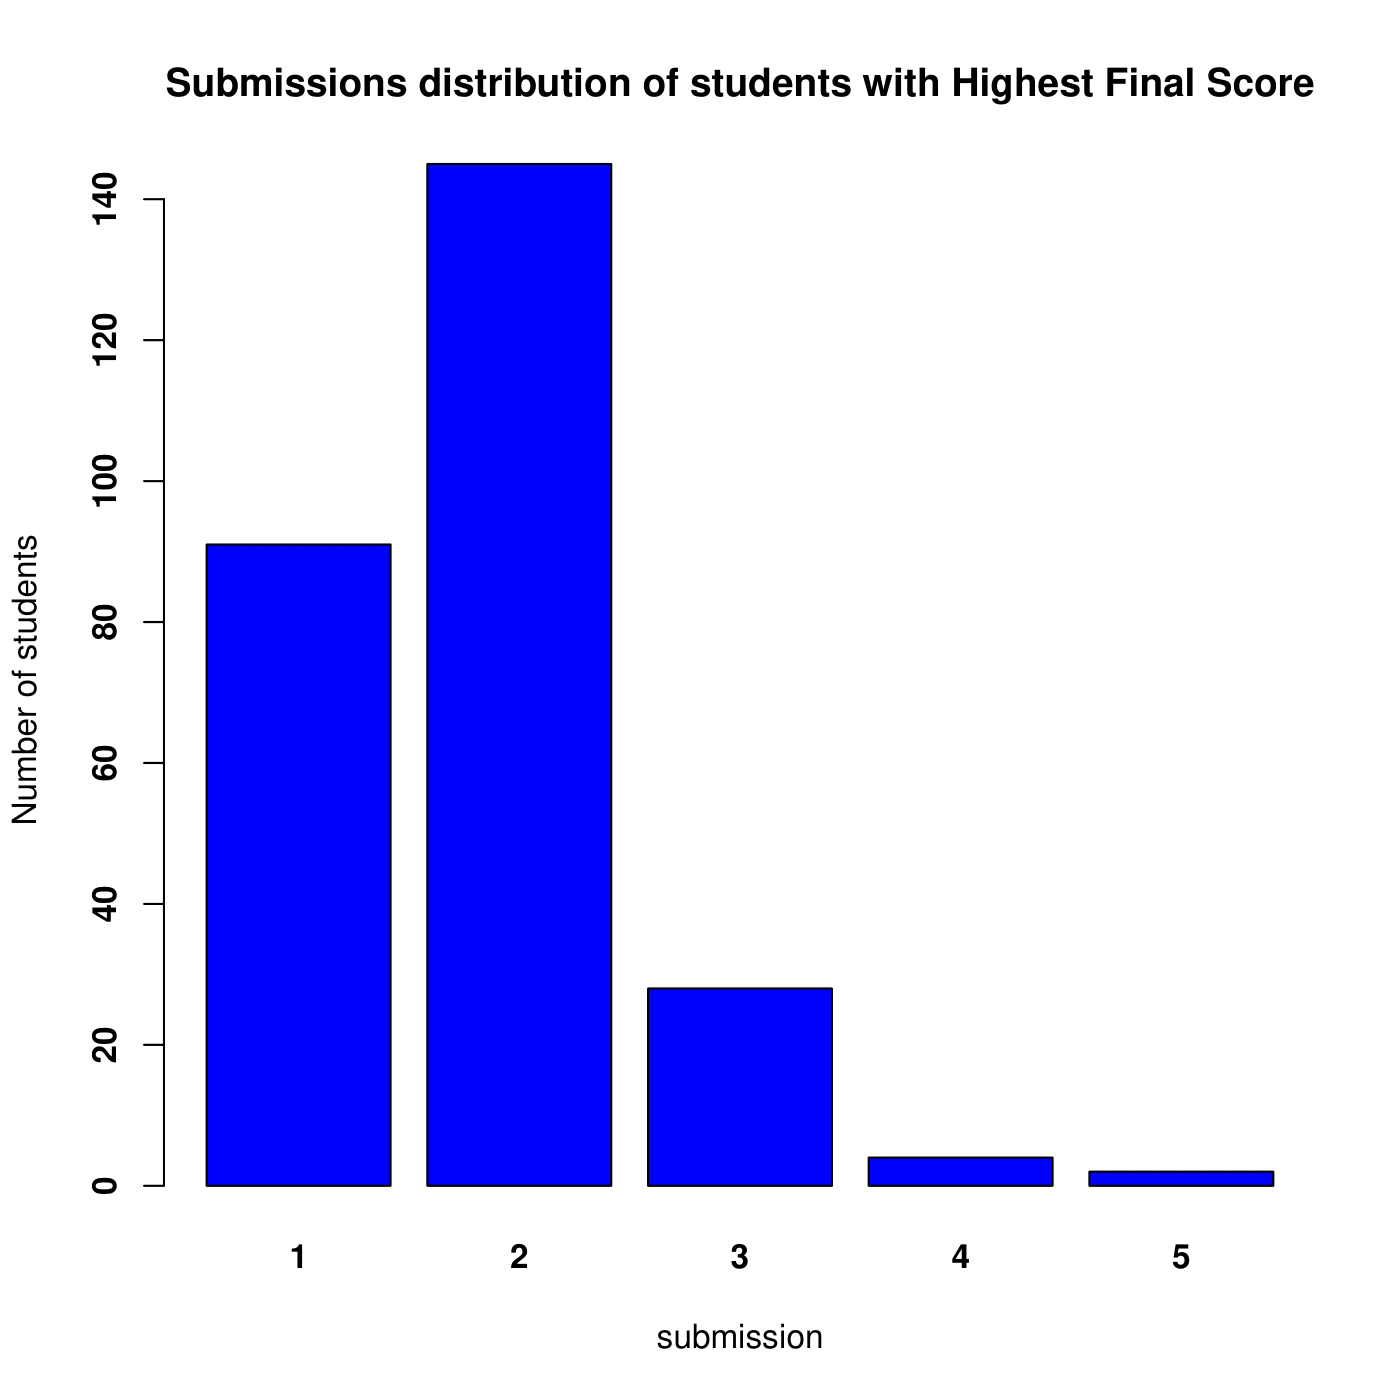
\includegraphics[width = 6.9cm]{Images/img2-4-1.png} & 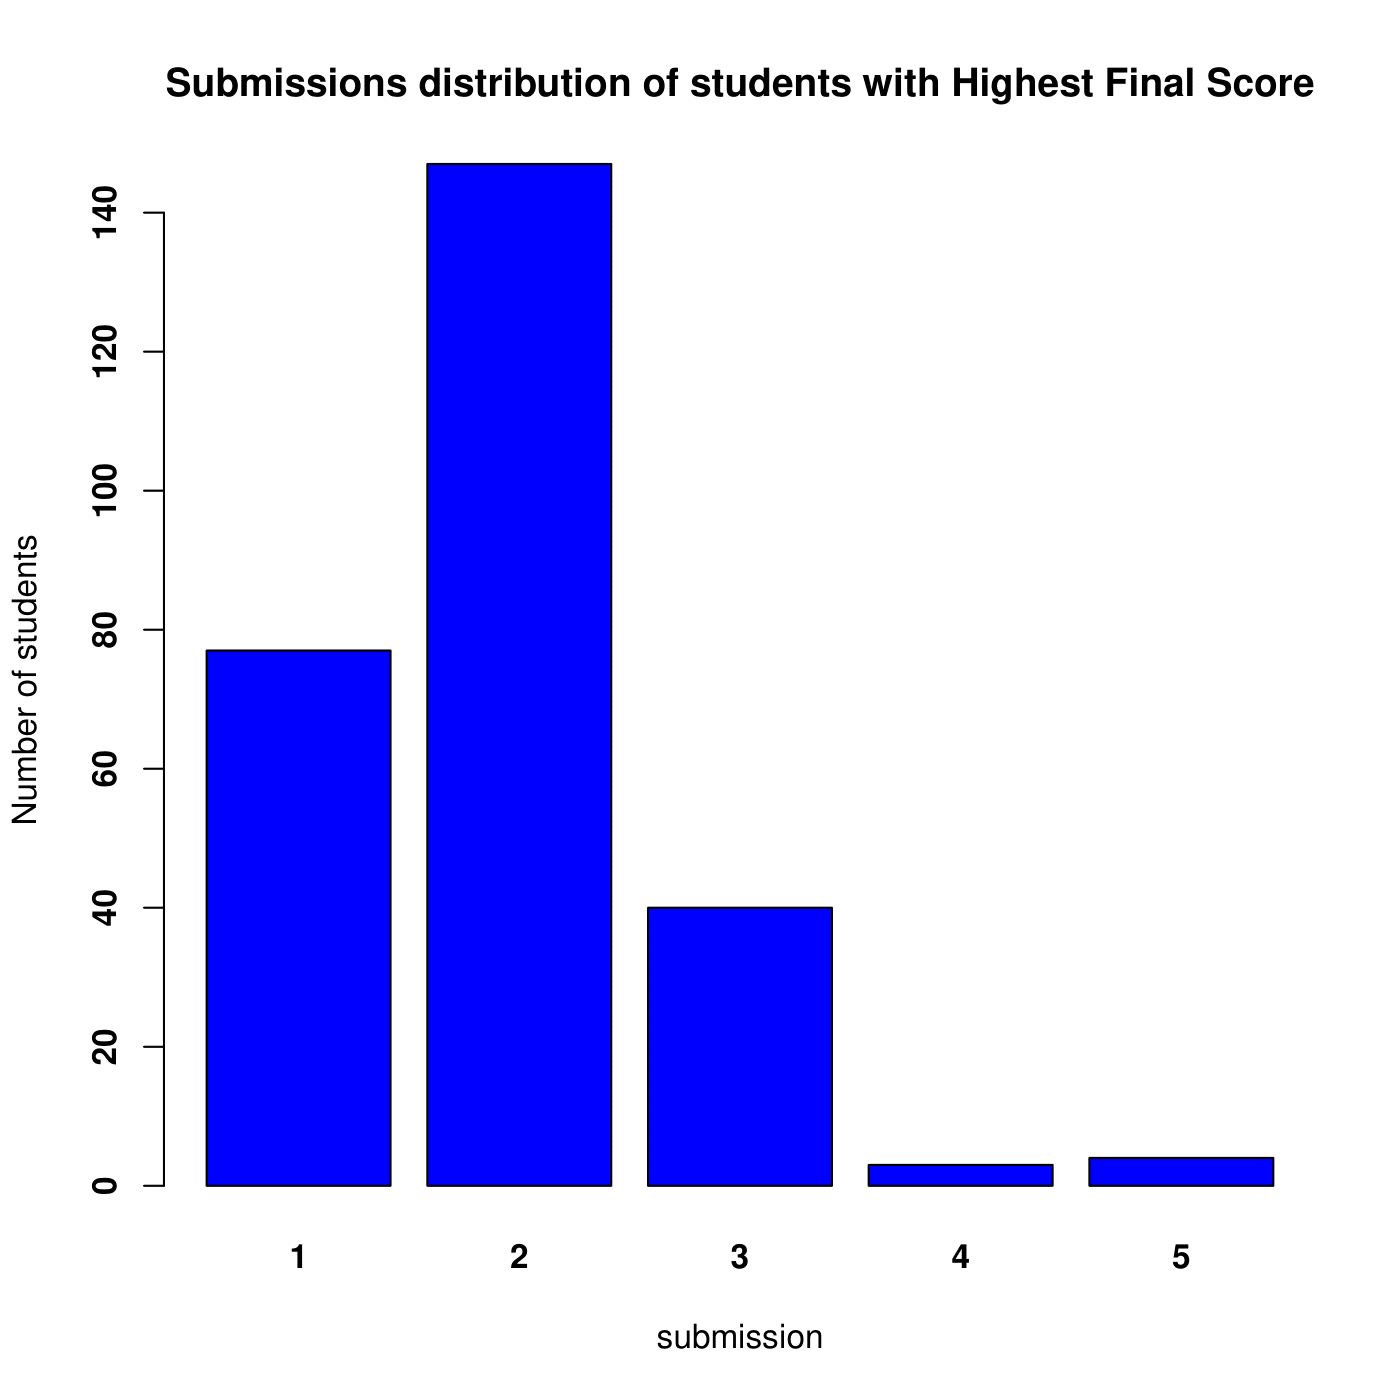
\includegraphics[width = 6.9cm]{Images/img2-4-2.png} \\
                 (1) & (2) \\
                 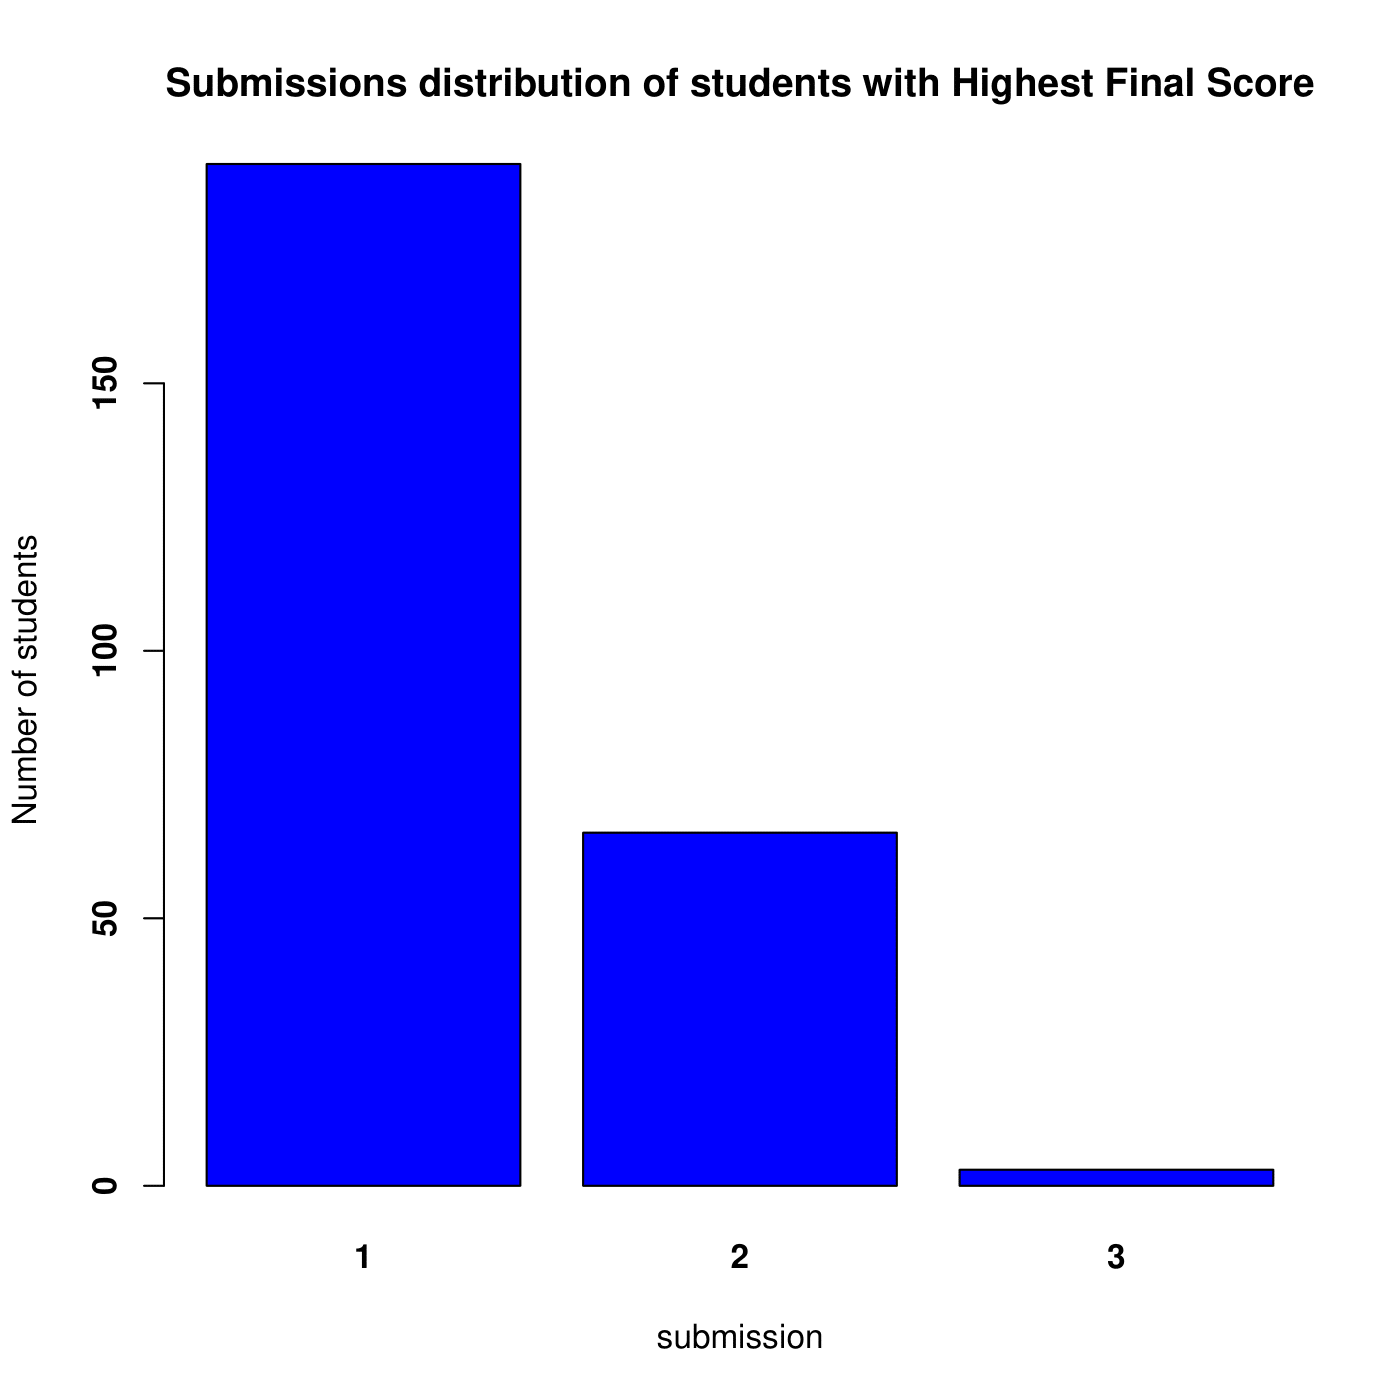
\includegraphics[width = 6.9cm]{Images/img2-4-3.png} &
                 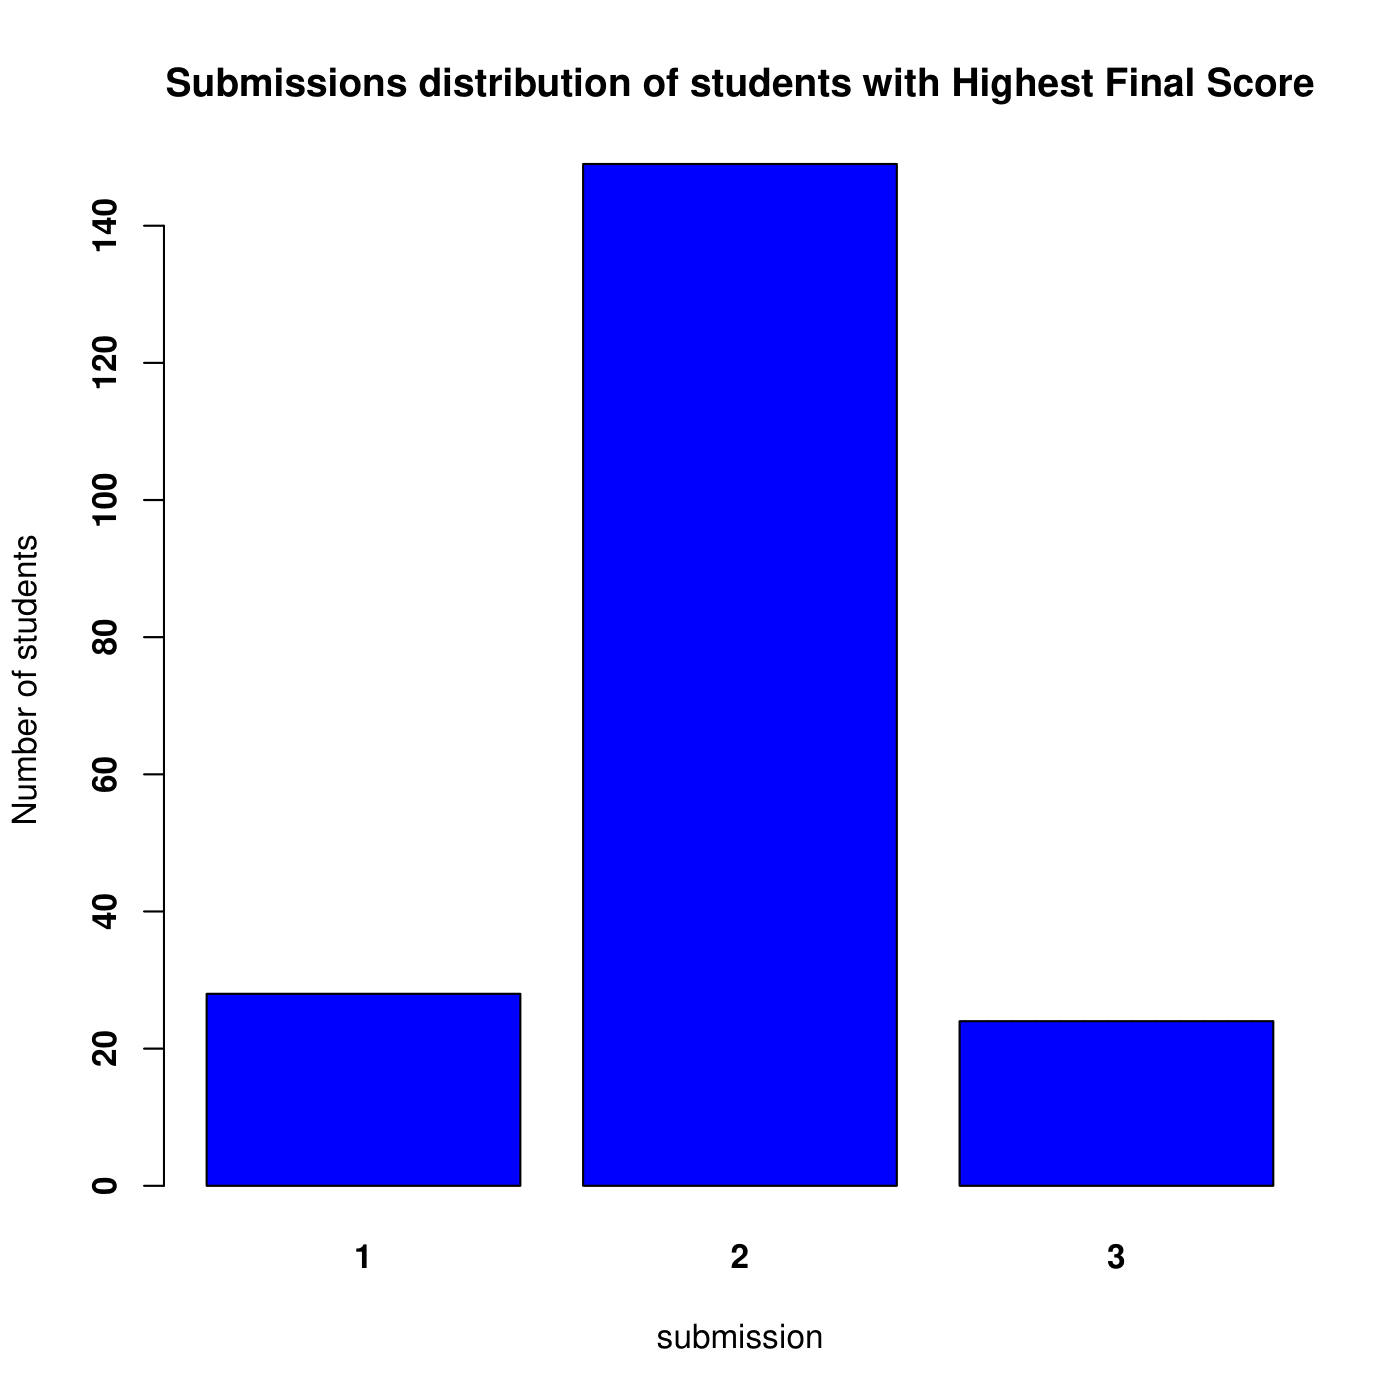
\includegraphics[width = 6.9cm]{Images/img2-4-4.png} \\
                 (3) & (4)
            \end{tabular}\\
            \textbf{Hình 2.4:} Phổ theo số lần nộp bài của các sinh viên có điểm số tổng kết cao nhất\\
            \begin{tabular}{c c}
                 (1) & \texttt{"CO1007\_TV\_HK192-Quiz 1.4-điểm.xlsx"}\\
                 (2) & \texttt{"CO1007\_TV\_HK192-Quiz 1.5-điểm.xlsx"}\\
                 (3) & \texttt{"CO1007\_TV\_HK192-Quiz 3.3-điểm.xlsx"}\\
                 (4) & \texttt{"CO1007\_TV\_HK192-Quiz 4.2-điểm.xlsx"}
            \end{tabular}
        \end{center}
    \end{itemize}
    %Cau n
    \bf\item Xác định điểm số trung bình của của các sinh viên trong mẫu\\[6pt]
    \bf Kiến thức chuẩn bị\normalfont
    \begin{itemize}
        \item Cách giải truyền thống:
        \begin{itemize}
            \item Điểm số trung bình được tính bằng tổng điểm tổng kết chia cho số lượng sinh viên trong tập.
            \begin{center}
                $\overline{x} = \frac{\sum\limits_{i = 1}^k x_i}{k}$\\
                \begin{tabular}{p{13cm}}
                    trong đó: $x_i$ là điểm tổng kết của sinh viên thứ $i$, $k$ là số lượng sinh viên.
                \end{tabular}
            \end{center}
        \end{itemize}
    \end{itemize}
    \bf Hiện thực trên R\normalfont
    \begin{itemize}
        \item Ý tưởng thực hiện:
        \begin{itemize}
            \item Ta sử dụng hàm $mean()$ để tính giá trị trung bình của điểm tổng kết.
            \begin{center}
                \begin{tabular}{p{13cm}}
                    \texttt{K.mean <- mean(List.Of.Final.Total\$Total)}
                \end{tabular}
            \end{center}
        \end{itemize}
        \item Kết quả:
        \begin{itemize}
            \item Điểm số trung bình của các sinh viên trong mỗi file:
            \begin{center}
                \begin{tabular}{l c}
                     \texttt{"CO1007\_TV\_HK192-Quiz 1.4-điểm.xlsx"} & 9.8\\
                     \texttt{"CO1007\_TV\_HK192-Quiz 1.5-điểm.xlsx"} & 9.8\\
                     \texttt{"CO1007\_TV\_HK192-Quiz 3.3-điểm.xlsx"} & 9.9\\
                     \texttt{"CO1007\_TV\_HK192-Quiz 4.2-điểm.xlsx"} & 9.8
                \end{tabular}
            \end{center}
        \end{itemize}
    \end{itemize}
    %Cau o
    \bf\item Xác định số lượng sinh viên có điểm số trung bình \\[6pt]
    \bf Kiến thức chuẩn bị\normalfont
    \begin{itemize}
        \item Cách giải truyền thống:
        \begin{itemize}
            \item Dựa vào danh sách điểm tổng kết đã tính ở trên và điểm trung bình ở câu n, ta lập danh sách những bạn có điểm tổng kết bằng điểm trung bình, sau đó đếm số lượng sinh viên trong danh sách này.
        \end{itemize}
    \end{itemize}
    \bf Hiện thực trên R\normalfont
    \begin{itemize}
        \item Ý tưởng thực hiện:
        \begin{itemize}
            \item Dùng hàm $subset()$ tạo một danh sách $List.mean$ là danh sách con của danh sách tổng kết với điều kiện là điểm tổng kết bằng với điểm trung bình.
            \begin{center}
                \begin{tabular}{p{13cm}}
                    \texttt{List.mean <- subset(List.Of.Final.Total, Total == K.mean)}
                \end{tabular}
            \end{center}
            \item Sau đó, ta sử dụng hàm $length()$ để lấy số lượng sinh viên thỏa mãn.
        \end{itemize}
        \item Kết quả:
        \begin{itemize}
            \item Số lượng sinh viên có điểm tổng kết bằng số điểm trung bình trong mỗi file:
            \begin{center}
                \begin{tabular}{l c}
                     \texttt{"CO1007\_TV\_HK192-Quiz 1.4-điểm.xlsx"} & 0 sinh viên\\
                     \texttt{"CO1007\_TV\_HK192-Quiz 1.5-điểm.xlsx"} & 0 sinh viên\\
                     \texttt{"CO1007\_TV\_HK192-Quiz 3.3-điểm.xlsx"} & 0 sinh viên\\
                     \texttt{"CO1007\_TV\_HK192-Quiz 4.2-điểm.xlsx"} & 0 sinh viên
                \end{tabular}
            \end{center}
        \end{itemize}
    \end{itemize}
    %Cau p
    \bf\item Tính trung vị mẫu, cực đại mẫu, cực tiểu mẫu của trên.\\[6pt]
    \bf Kiến thức chuẩn bị\normalfont
    \begin{itemize}
        \item Cách giải truyền thống:
        \begin{itemize}
            \item Trung vị: Là một số tách giữa nửa lớn hơn và nữa bé hơn của một mẫu, một quần thể, nhưng ở đây ta nói đến là một tập hợp các giá trị là điểm.
            \item Cực đại và cực tiểu: Là thành phần lớn nhất (hoặc cùng lớn nhất), nhỏ nhất (hoặc cùng nhỏ nhất) của một tập hợp các giá trị.
        \end{itemize}
    \end{itemize}
    \bf Hiện thực trên R\normalfont
    \begin{itemize}
        \item Ý tưởng thực hiện:
        \begin{itemize}
            \item Ta sử dụng các hàm $median()$, $min()$, $max()$ để tìm các giá trị tương ứng.
            \begin{center}
                \begin{tabular}{p{13cm}}
                    \texttt{print(median(K\$Total))} \\
                    \texttt{print(min(K\$Total))} \\
                    \texttt{print(max(K\$Total))}
                \end{tabular}
            \end{center}
        \end{itemize}
        \item Kết quả:
        \begin{itemize}
            \item Trung vị mẫu, cực đại mẫu và cực tiểu mẫu trong mỗi file:
            \begin{center}
                \begin{tabular}{l c c c}
                     & Trung vị & Cực đại & Cực tiểu\\
                     \texttt{"CO1007\_TV\_HK192-Quiz 1.4-điểm.xlsx"} & 9.67 & 10 & 4.5\\
                     \texttt{"CO1007\_TV\_HK192-Quiz 1.5-điểm.xlsx"} & 9.5 & 10 & 0.5\\
                     \texttt{"CO1007\_TV\_HK192-Quiz 3.3-điểm.xlsx"} & 10 & 10 & 0\\
                     \texttt{"CO1007\_TV\_HK192-Quiz 4.2-điểm.xlsx"} & 9.5 & 10 & 0
                \end{tabular}
            \end{center}
        \end{itemize}
    \end{itemize}
    %Cau q
    \bf\item Hãy đo mức độ phân tán của điểm số (xung quanh giá trị trung bình) của  mẫu\\[6pt]
    \bf Kiến thức chuẩn bị\normalfont
    \begin{itemize}
        \item Cách giải truyền thống:
        \begin{itemize}
            \item Độ phân tán được xác định bằng phương sai - độ lệch chuẩn của mẫu.
            \item Phương sai được tính bằng công thức:
            \begin{center}
                $s^2 = \frac{1}{n} \sum \limits_{i=1}^{k} n_i x_i^2 - \overline{x}^2$
                \begin{tabular}{p{13cm}}
                    \begin{tabular}{l l}
                        trong đó: & $x_i$ là điểm số có tần số $n_i$\\
                        & $k$ là số các các trị $x_i$ phân biệt\\
                        & $n$ là tổng số bài làm\\
                        & $\overline{x}$ là giá trị điểm trung bình
                    \end{tabular}
                \end{tabular}
            \end{center}
            \item Độ lệch chuẩn được tính bằng công thức:
            \begin{center}
                $s = \sqrt{s^2}$
            \end{center}
        \end{itemize}
    \end{itemize}
    \bf Hiện thực trên R\normalfont
    \begin{itemize}
        \item Ý tưởng thực hiện:
        \begin{itemize}
            \item Ta sử dụng hàm $var()$ và $sd()$ để tính các giá trị tương ứng của mẫu.
            \begin{center}
                \begin{tabular}{p{13cm}}
                    \texttt{print(var(K\$Total))} \\
                    \texttt{print(sd(K\$Total))}
                \end{tabular}
            \end{center}
        \end{itemize}
        \item Kết quả:
        \begin{itemize}
            \item Phương sai, độ lệch chuẩn của  mẫu trong mỗi file:
            \begin{center}
                \begin{tabular}{l c c}
                     & Phương sai & Độ lệch chuẩn\\
                     \texttt{"CO1007\_TV\_HK192-Quiz 1.4-điểm.xlsx"} & 0.8145266 & 0.9025113\\
                     \texttt{"CO1007\_TV\_HK192-Quiz 1.5-điểm.xlsx"} & 1.238846 & 1.113034\\
                     \texttt{"CO1007\_TV\_HK192-Quiz 3.3-điểm.xlsx"} & 0.6682011 & 0.8174357\\
                     \texttt{"CO1007\_TV\_HK192-Quiz 4.2-điểm.xlsx"} & 1.874935 & 1.369283
                \end{tabular}
            \end{center}
        \end{itemize}
    \end{itemize}.
    %Cau r
    \bf\item Tính độ méo lệch (skewness), và độ nhọn (kurtosis) của dữ liệu trong mẫu trên.\\[6pt]
    \bf Kiến thức chuẩn bị\normalfont
    \begin{itemize}
        \item Cách giải truyền thống:
        \begin{itemize}
            \item Độ méo lệch là sự biến dạng sự bất đối xứng trong một phân phối hình chuông đối xứng hay phân phối chuẩn trong một tập dữ liệu, được tính bằng công thức:
            \begin{center}
                $\tilde{\mu}_3 = \frac{1}{n} \sum \limits_{i=1}^{k} n_i (\frac{x_i - \overline{x}}{s})^3$
                \begin{tabular}{p{13cm}}
                    \begin{tabular}{l l}
                        trong đó: & $x_i$ là điểm số có tần số $n_i$\\
                        & $k$ là số các các trị $x_i$ phân biệt\\
                        & $n$ là tổng số bài làm\\
                        & $\overline{x}$ là giá trị điểm trung bình\\
                        & $s$ là độ lệch chuẩn
                    \end{tabular}
                \end{tabular}
            \end{center}
            \item Độ nhọn là một đại lượng thống kê được sử dụng để miêu tả các phân phối, mô tả hình dạng của đuôi phân phối đó, tính bằng công thức.
            \begin{center}
                $\tilde{\mu}_4 = \frac{1}{n} \sum \limits_{i=1}^{k} n_i (\frac{x_i - \overline{x}}{s})^4$
                \begin{tabular}{p{13cm}}
                    \begin{tabular}{l l}
                        trong đó: & $x_i$ là điểm số có tần số $n_i$\\
                        & $k$ là số các các trị $x_i$ phân biệt\\
                        & $n$ là tổng số bài làm\\
                        & $\overline{x}$ là giá trị điểm trung bình\\
                        & $s$ là độ lệch chuẩn
                    \end{tabular}
                \end{tabular}
            \end{center}
        \end{itemize}
    \end{itemize}
    \bf Hiện thực trên R\normalfont
    \begin{itemize}
        \item Ý tưởng thực hiện:
        \begin{itemize}
            \item Ta sử dụng hàm $skewness()$ và hàm $kurtosis()$ để tính các giá trị tương ứng.
            \begin{center}
                \begin{tabular}{p{13cm}}
                    \texttt{print(skewness(List.Of.Final.Total\$Total))} \\
                    \texttt{print(kurtosis(List.Of.Final.Total\$Total))}
                \end{tabular}
            \end{center}
        \end{itemize}
        \item Kết quả:
        \begin{itemize}
            \item Độ méo lệch, độ nhọn của  mẫu trong mỗi file:
            \begin{center}
                \begin{tabular}{l c c}
                     & Độ méo lệch & Độ nhọn\\
                     \texttt{"CO1007\_TV\_HK192-Quiz 1.4-điểm.xlsx"} & -1.507457 & 5.730385\\
                     \texttt{"CO1007\_TV\_HK192-Quiz 1.5-điểm.xlsx"} & -2.62223 & 15.32753\\
                     \texttt{"CO1007\_TV\_HK192-Quiz 3.3-điểm.xlsx"} & -6.303646 & 64.30899\\
                     \texttt{"CO1007\_TV\_HK192-Quiz 4.2-điểm.xlsx"} & -1.601421 & 7.084802
                \end{tabular}
            \end{center}
        \end{itemize}
    \end{itemize}
    %Cau s
    \bf\item Tính tứ phân vị (quartile) thứ nhất ($Q_1$) và thứ ba ($Q_3$) của mẫu.\\[6pt]
    \bf Kiến thức chuẩn bị\normalfont
    \begin{itemize}
        \item Cách giải truyền thống:
        \begin{itemize}
            \item Tứ phân vị thứ nhất $Q_1$: bằng trung vị phần dưới của một tập.
            \item Tứ phân vị thứ hai $Q_3$: bằng trung vị phần trên của một tập.
        \end{itemize}
    \end{itemize}
    \bf Hiện thực trên R\normalfont
    \begin{itemize}
        \item Ý tưởng thực hiện:
        \begin{itemize}
            \item Ta sử dụng hàm $quantile()$ với các tham số truyền vào là 0.25 và 0.75 tương ứng.
            \begin{center}
                \begin{tabular}{p{13cm}}
                    \texttt{print(quantile(K\$Total, 0.25))} \\
                    \texttt{print(quantile(K\$Total, 0.75))}
                \end{tabular}
            \end{center}
        \end{itemize}
        \item Kết quả:
        \begin{itemize}
            \item Tứ phân vị thứ nhất và thứ ba trong mỗi file:
            \begin{center}
                \begin{tabular}{l c c}
                     & Thứ nhất $Q_1$ & Thứ ba $Q_3$\\
                     \texttt{"CO1007\_TV\_HK192-Quiz 1.4-điểm.xlsx"} & 9 & 10\\
                     \texttt{"CO1007\_TV\_HK192-Quiz 1.5-điểm.xlsx"} & 9 & 10\\
                     \texttt{"CO1007\_TV\_HK192-Quiz 3.3-điểm.xlsx"} & 9 & 10\\
                     \texttt{"CO1007\_TV\_HK192-Quiz 4.2-điểm.xlsx"} & 8 & 10
                \end{tabular}
            \end{center}
        \end{itemize}
    \end{itemize}
    %Cau t
    \bf\item {Xác định số lượng sinh viên có điểm số nằm trong 2 mức điểm cao nhất}\\[6pt]
    \bf Kiến thức chuẩn bị\normalfont
    \begin{itemize}
        \item Cách giải truyền thống:
        \begin{itemize}
            \item Từ danh sách điểm tổng kết, ta loại bỏ những bạn có số điểm cao nhất, sau đó tiến hành tìm những bạn có số điểm cao nhất trong danh sách này. Những bạn này chính là những bạn có số điểm cao thứ hai.
        \end{itemize}
    \end{itemize}
    \bf Hiện thực trên R\normalfont
    \begin{itemize}
        \item Ý tưởng thực hiện:
        \begin{itemize}
            \item Ta sử dụng hàm $max()$ kèm theo điều kiện điểm số khác điểm cao nhất để xác định mức điểm cao thứ hai.
            \begin{center}
                \begin{tabular}{p{13cm}}
                    \texttt{Second.Highest.Final.Total <- max(List.Of.Final.Total\$Total [List.Of.Final.Total\$Total != Highest.Final.Total])}
                \end{tabular}
            \end{center}
            \item $Second.Highest.Final.Total$ ở đây là điểm cao thứ hai trong danh sách.
            \item Ta tiếp tục sử dụng hàm $subset()$ để lập danh sách các bạn có điểm số lớn hơn hoặc bằng giá trị vừa tìm được.
            \begin{center}
                \begin{tabular}{p{13cm}}
                    \texttt{List.2Highest.Final.Total <- subset(List.Of.Final.Total, Total == Highest.Final.Total | Total == Second.Highest.Final.Total)}
                \end{tabular}
            \end{center}
            \item $List.2Highest.Final.Total$ là danh sách những bạn có điểm trong hai mức điểm cao nhất. 
            \item Sử dụng hàm $length()$, ta xác định được số lượng sinh viên trong nhóm này.
        \end{itemize}
        \item Kết quả:
        \begin{itemize}
            \item Số lượng sinh viên có điểm số nằm trong 2 mức điểm cao nhất trong mỗi file:
            \begin{center}
                \begin{tabular}{l c}
                     \texttt{"CO1007\_TV\_HK192-Quiz 1.4-điểm.xlsx"} & 287 sinh viên\\
                     \texttt{"CO1007\_TV\_HK192-Quiz 1.5-điểm.xlsx"} & 297 sinh viên\\
                     \texttt{"CO1007\_TV\_HK192-Quiz 3.3-điểm.xlsx"} & 277 sinh viên\\
                     \texttt{"CO1007\_TV\_HK192-Quiz 4.2-điểm.xlsx"} & 222 sinh viên
                \end{tabular}
            \end{center}
        \end{itemize}
    \end{itemize}
    %Cau u
    \bf\item {Xác định phổ theo số lần nộp bài của các sinh viên có điểm số tổng kết ở 2 mức điểm cao nhất}\\[6pt]
    \bf Kiến thức chuẩn bị\normalfont
    \begin{itemize}
        \item Cách giải truyền thống:
        \begin{itemize}
            \item Từ danh sách điểm tổng kết, kết hợp với hai giá trị là điểm cao nhất và điểm cao thứ hai, ta lọc ra những bạn thỏa điều kiện và vẽ phổ theo số lần nộp bài dựa trên dữ liệu vừa lọc được.
        \end{itemize}
    \end{itemize}
    \bf Hiện thực trên R\normalfont
    \begin{itemize}
        \item Ý tưởng thực hiện:
        \begin{itemize}
            \item Ta sử dụng hàm $subset()$ để tạo danh sách mới thỏa mãn điểm số bằng điểm cao nhất hoặc coa thứ hai, sau đó sử dụng hàm $table()$ để lập danh sách số lần nộp bài ứng với mỗi sinh viên.
            \begin{center}
                \begin{tabular}{p{13cm}}
                    \texttt{List.2Highest.Final.Total2 <-subset(K, ID \%in\% List.2Highest.Final.Total\$ID)} \\
                    \texttt{List.2Highest.Final.Total.Freq <- data.frame(table( List.2Highest.Final.Total2\$ID))}
                \end{tabular}
            \end{center}
            \item Sau đó ta dùng hàm $barplot()$ để vẽ phổ theo số lần nộp bài của các sinh viên có điểm số tổng kết ở 2 mức điểm cao nhất.
        \end{itemize}
        \item Biểu đồ:\\
        \begin{center}
            \begin{tabular}{c c}
                 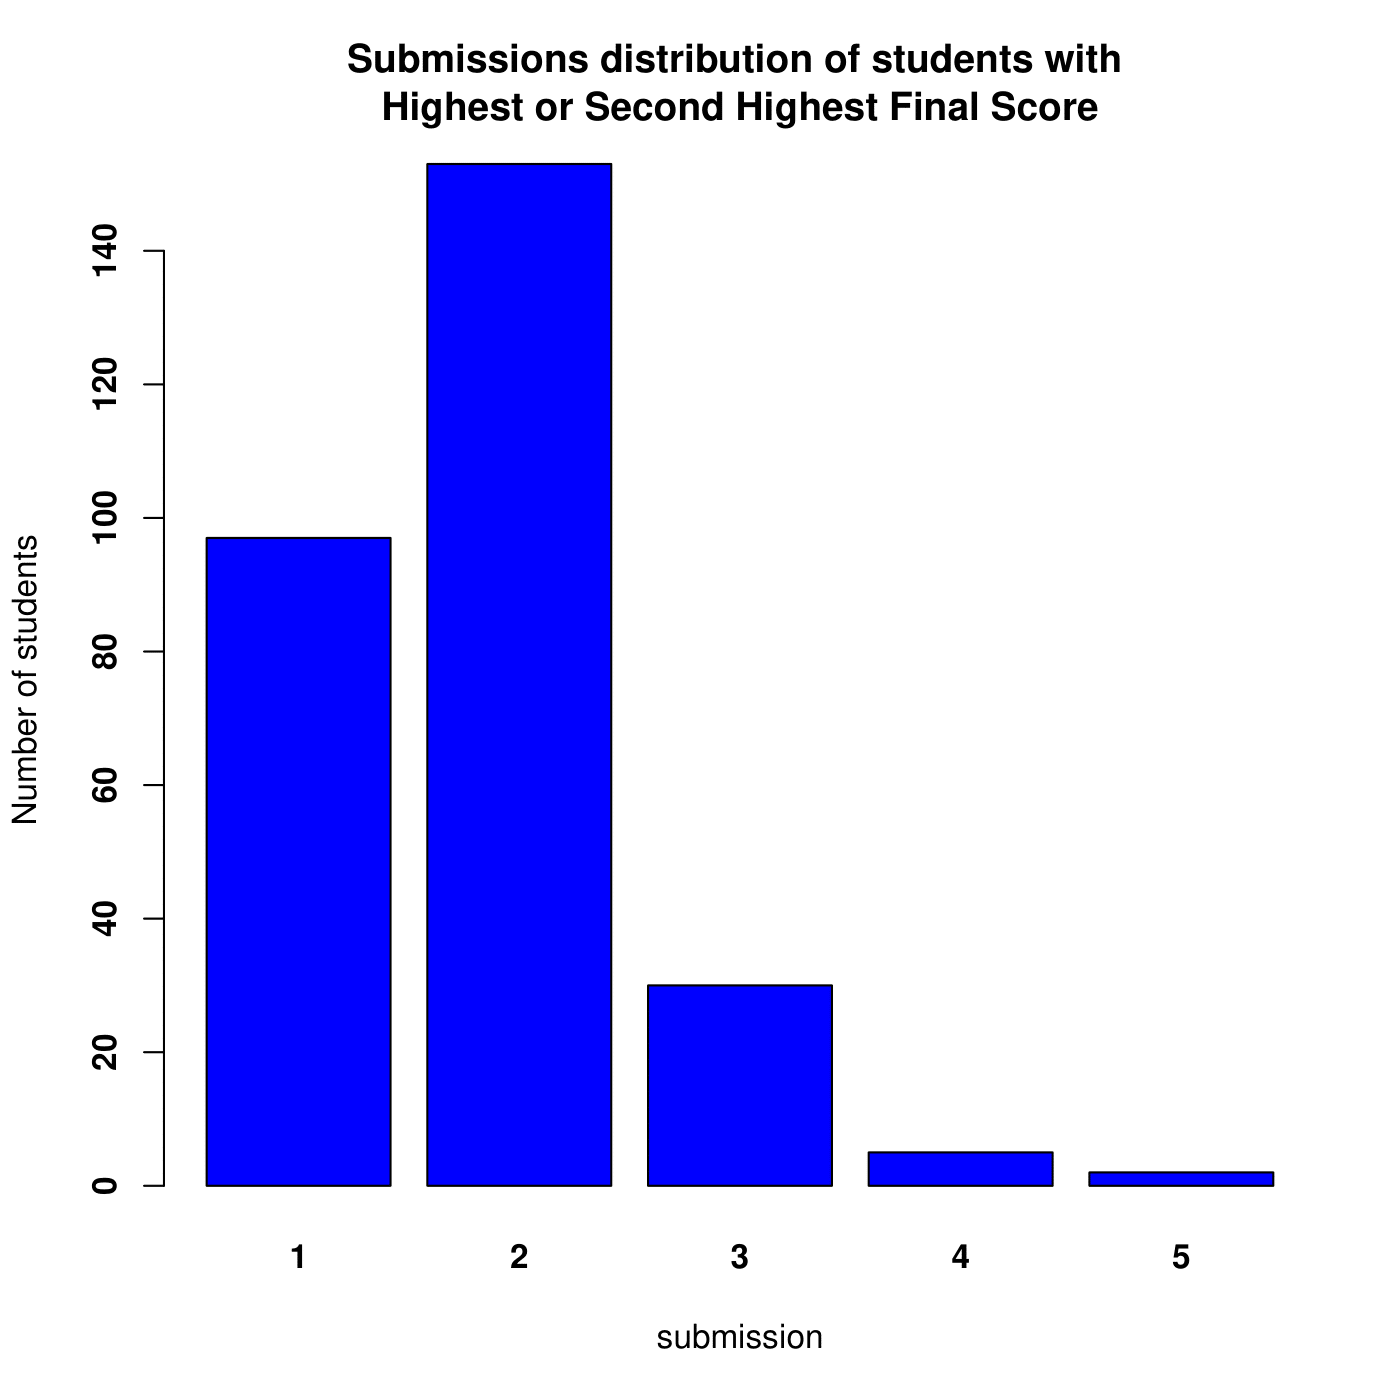
\includegraphics[width = 6.9cm]{Images/img2-5-1.png} & 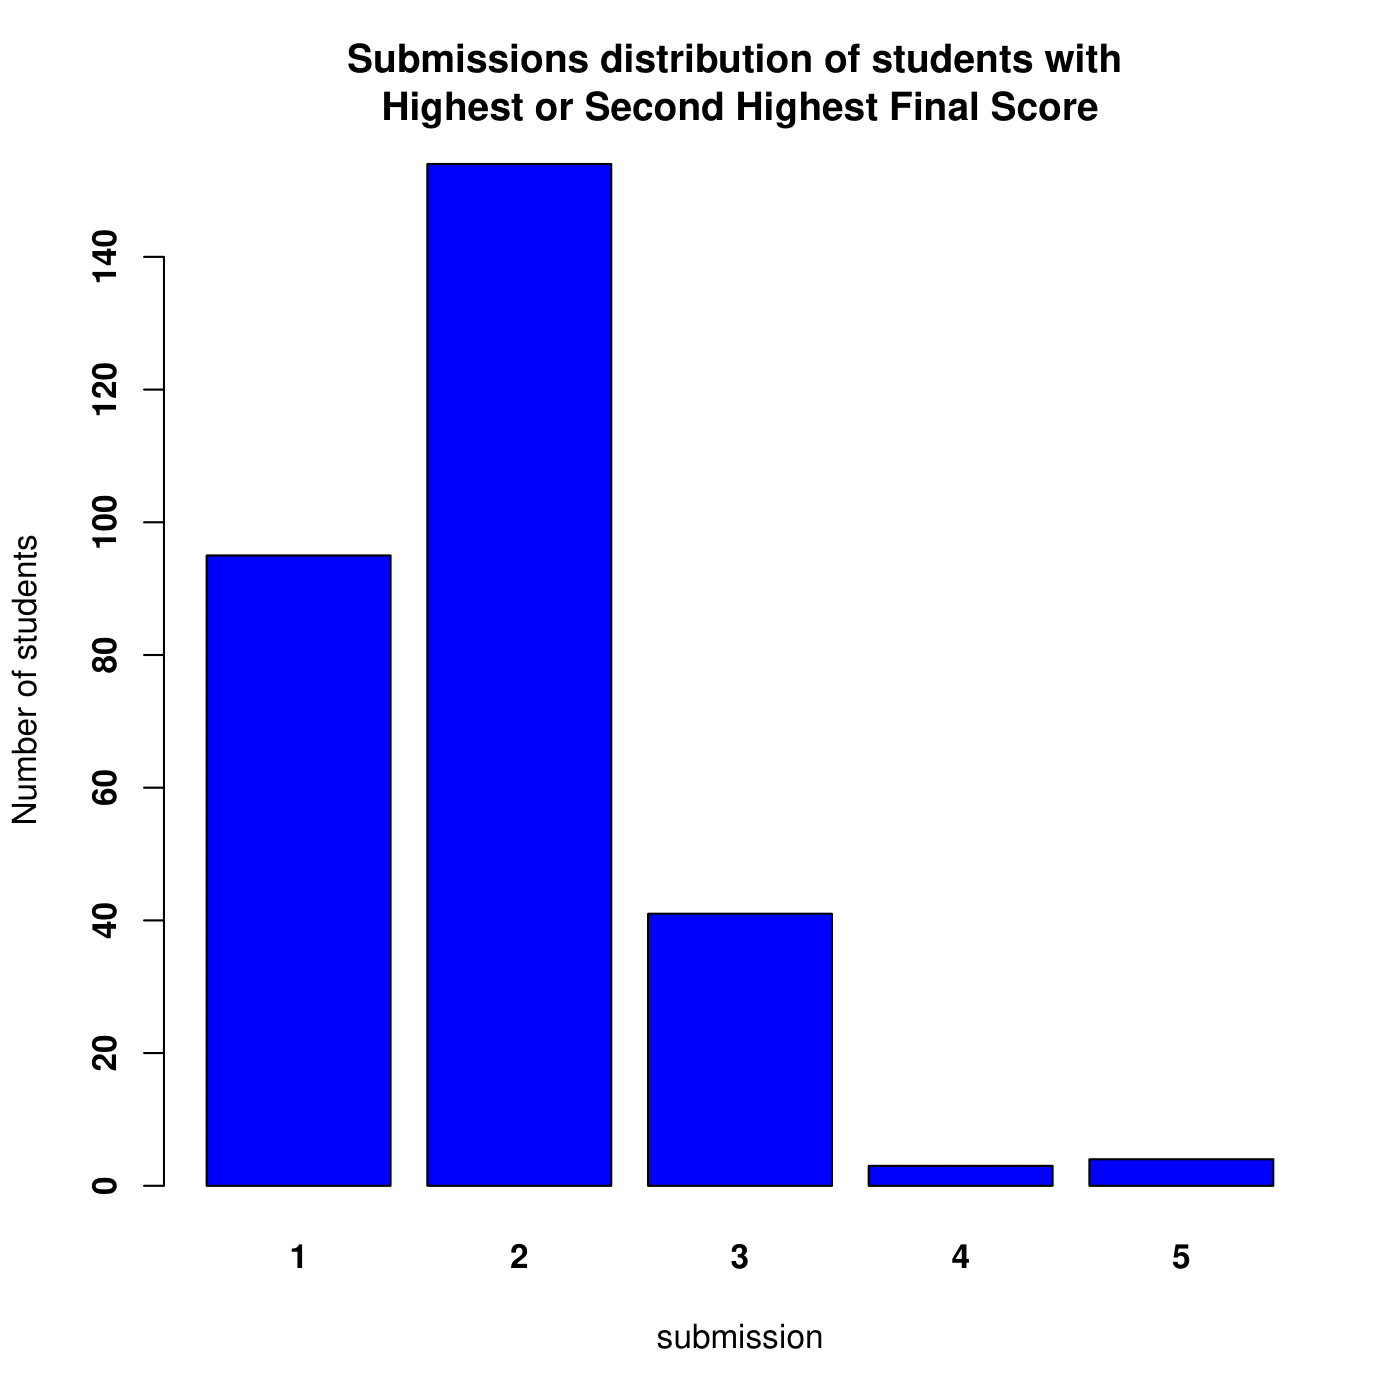
\includegraphics[width = 6.9cm]{Images/img2-5-2.png} \\
                 (1) & (2) \\
                 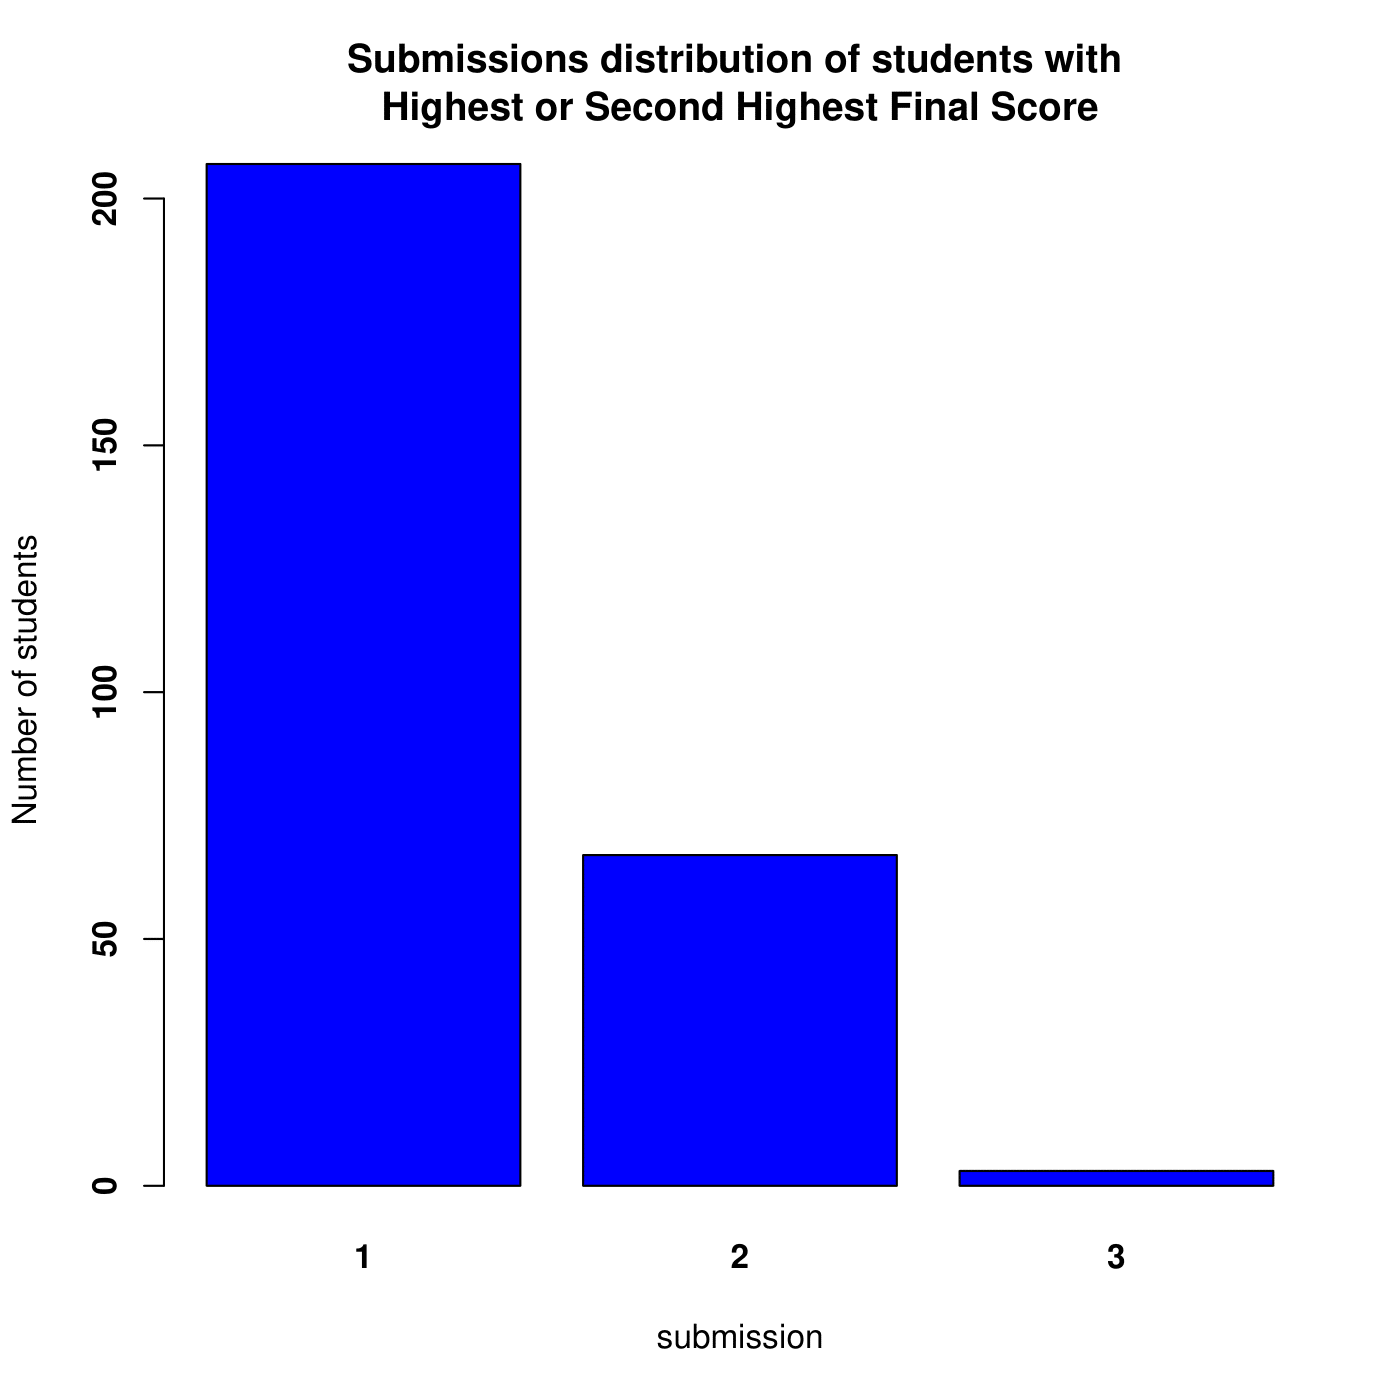
\includegraphics[width = 6.9cm]{Images/img2-5-3.png} &
                 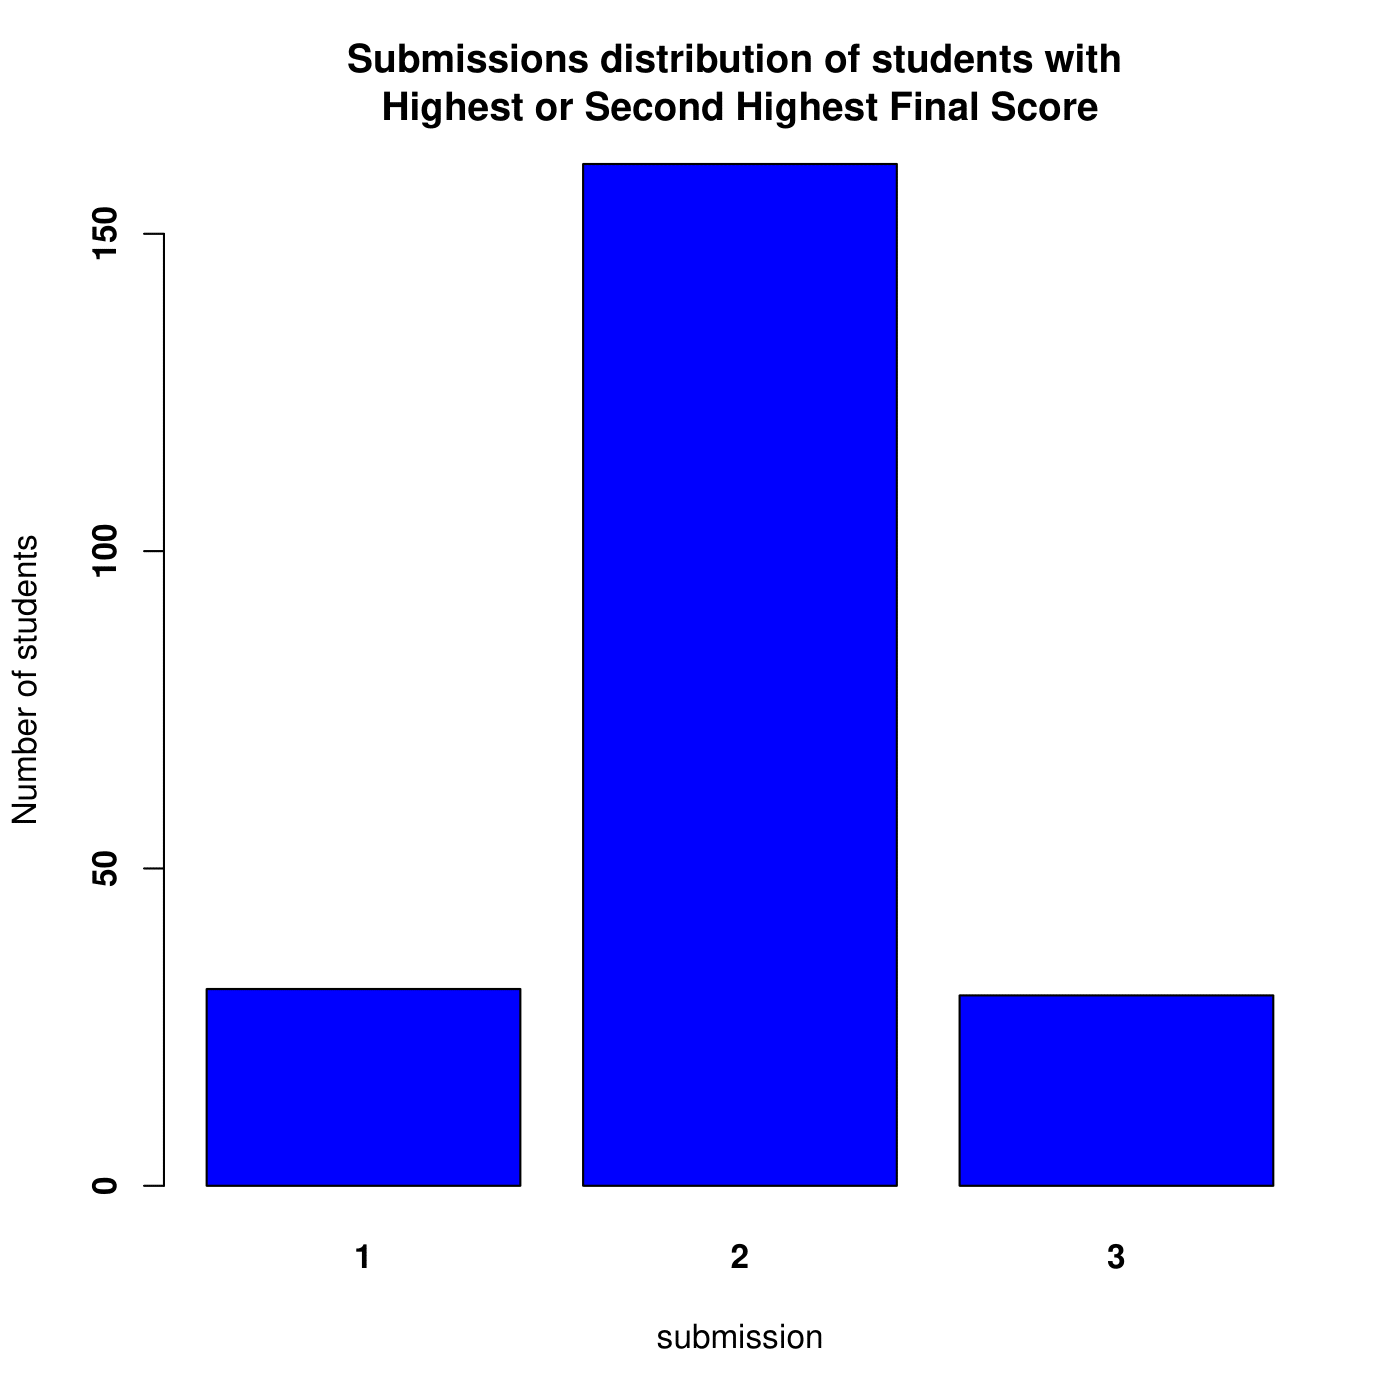
\includegraphics[width = 6.9cm]{Images/img2-5-4.png} \\
                 (3) & (4)
            \end{tabular}\\
            \textbf{Hình 2.5:} Phổ theo số lần nộp bài của các sinh viên có điểm số tổng kết ở 2 mức điểm cao nhất\\
            \begin{tabular}{c c}
                 (1) & \texttt{"CO1007\_TV\_HK192-Quiz 1.4-điểm.xlsx"}\\
                 (2) & \texttt{"CO1007\_TV\_HK192-Quiz 1.5-điểm.xlsx"}\\
                 (3) & \texttt{"CO1007\_TV\_HK192-Quiz 3.3-điểm.xlsx"}\\
                 (4) & \texttt{"CO1007\_TV\_HK192-Quiz 4.2-điểm.xlsx"}
            \end{tabular}
        \end{center}
    \end{itemize}
    %Cau v
    \bf\item {Xác định số lượng sinh viên có điểm số tổng kết ở mức điểm cao thứ $k$ với $k$ cho trước\\[6pt]
    \bf Kiến thức chuẩn bị\normalfont
    \begin{itemize}
        \item Cách giải truyền thống:
        \begin{itemize}
            \item Từ dữ liệu ban đầu, ta lập dãy điểm tổng kết xếp từ cao xuống thấp, lấy giá trị thứ $k$ của dãy ta vừa lập. Dựa vào giá trị này, ta lập danh sách các sinh viên có điểm tổng kết bằng giá trị này, sau đó tính số lượng các sinh viên thỏa mãn.
        \end{itemize}
    \end{itemize}
    \bf Hiện thực trên R\normalfont
    \begin{itemize}
        \item Ý tưởng thực hiện:
        \begin{itemize}
            \item Ta sử dụng tổ hợp hai hàm $unique()$ và $order()$ để lập dãy điểm tổng từ dữ liệu ban đầu, sau đó lấy phần tử thứ $k$ từ dãy vừa lập.
            \begin{center}
                \begin{tabular}{p{13cm}}
                    \texttt{Total.Descending <- unique(List.Of.Final.Total[order( -List.Of.Final.Total\$Total), ]\$Total)}\\
                    \texttt{Certain.Total <- Total.Descending[k]}
                \end{tabular}
            \end{center}
            \item Sau đó, ta sử dụng hàm $subset()$ để lọc ra các sinh viên thỏa mãn điểm tổng kết bằng mức điểm vừa tìm được và sử dụng hàm $nrow()$ để tính số lượng tương ứng.
        \end{itemize}
        \item Kết quả:
        \begin{itemize}
            \item Giả sử $k = 2$
            \item Số lượng sinh viên có điểm số nằm trong mức điểm thứ $k$ trong mỗi file:
            \begin{center}
                \begin{tabular}{l c}
                     \texttt{"CO1007\_TV\_HK192-Quiz 1.4-điểm.xlsx"} & 17 sinh viên\\
                     \texttt{"CO1007\_TV\_HK192-Quiz 1.5-điểm.xlsx"} & 26 sinh viên\\
                     \texttt{"CO1007\_TV\_HK192-Quiz 3.3-điểm.xlsx"} & 17 sinh viên\\
                     \texttt{"CO1007\_TV\_HK192-Quiz 4.2-điểm.xlsx"} & 21 sinh viên
                \end{tabular}
            \end{center}
        \end{itemize}
    \end{itemize}}
    %Cau w
    \bf\item {Xác định phổ theo số lần nộp bài của các sinh viên có điểm số tổng kết ở mức điểm cao thứ $k$ với $k$ cho trước}\\[6pt]
    \bf Kiến thức chuẩn bị\normalfont
    \begin{itemize}
        \item Cách giải truyền thống:
        \begin{itemize}
            \item Từ dữ liệu ban đầu, ta lập danh sách toàn bộ các lần nộp của các sinh viên thỏa mãn điều kiện điểm tổng kết bằng mức điểm vừa tìm được, sau đó lập bảng các sinh viên đó kèm theo số lần nộp bài. Từ đó, ta vẽ được phổ theo số lần nộp bài của nhóm sinh viên này.
        \end{itemize}
    \end{itemize}
    \bf Hiện thực trên R\normalfont
    \begin{itemize}
        \item Ý tưởng thực hiện:
        \begin{itemize}
            \item Ta sử dụng tổ hợp hai hàm $unique()$ và $order()$ để lập danh sách toàn bộ các lần nộp của các sinh viên thỏa mãn điều kiện điểm tổng kết bằng mức điểm vừa tìm được. Sau đó, ta sử dụng hàm $table()$ để tạo một dataframe mới gồm các sinh viên thỏa mãn cùng số lần mỗi sinh viên nộp bài.
            \item Cuối cùng, ta sử dụng hàm $barplot()$ để vẽ được phổ theo số lần nộp bài của nhóm sinh viên này.
        \end{itemize}
        \item Biểu đồ:
        \begin{center}
            \begin{itemize}
                \item Giả sử $k = 2$
            \end{itemize}
            \begin{tabular}{c c}
                 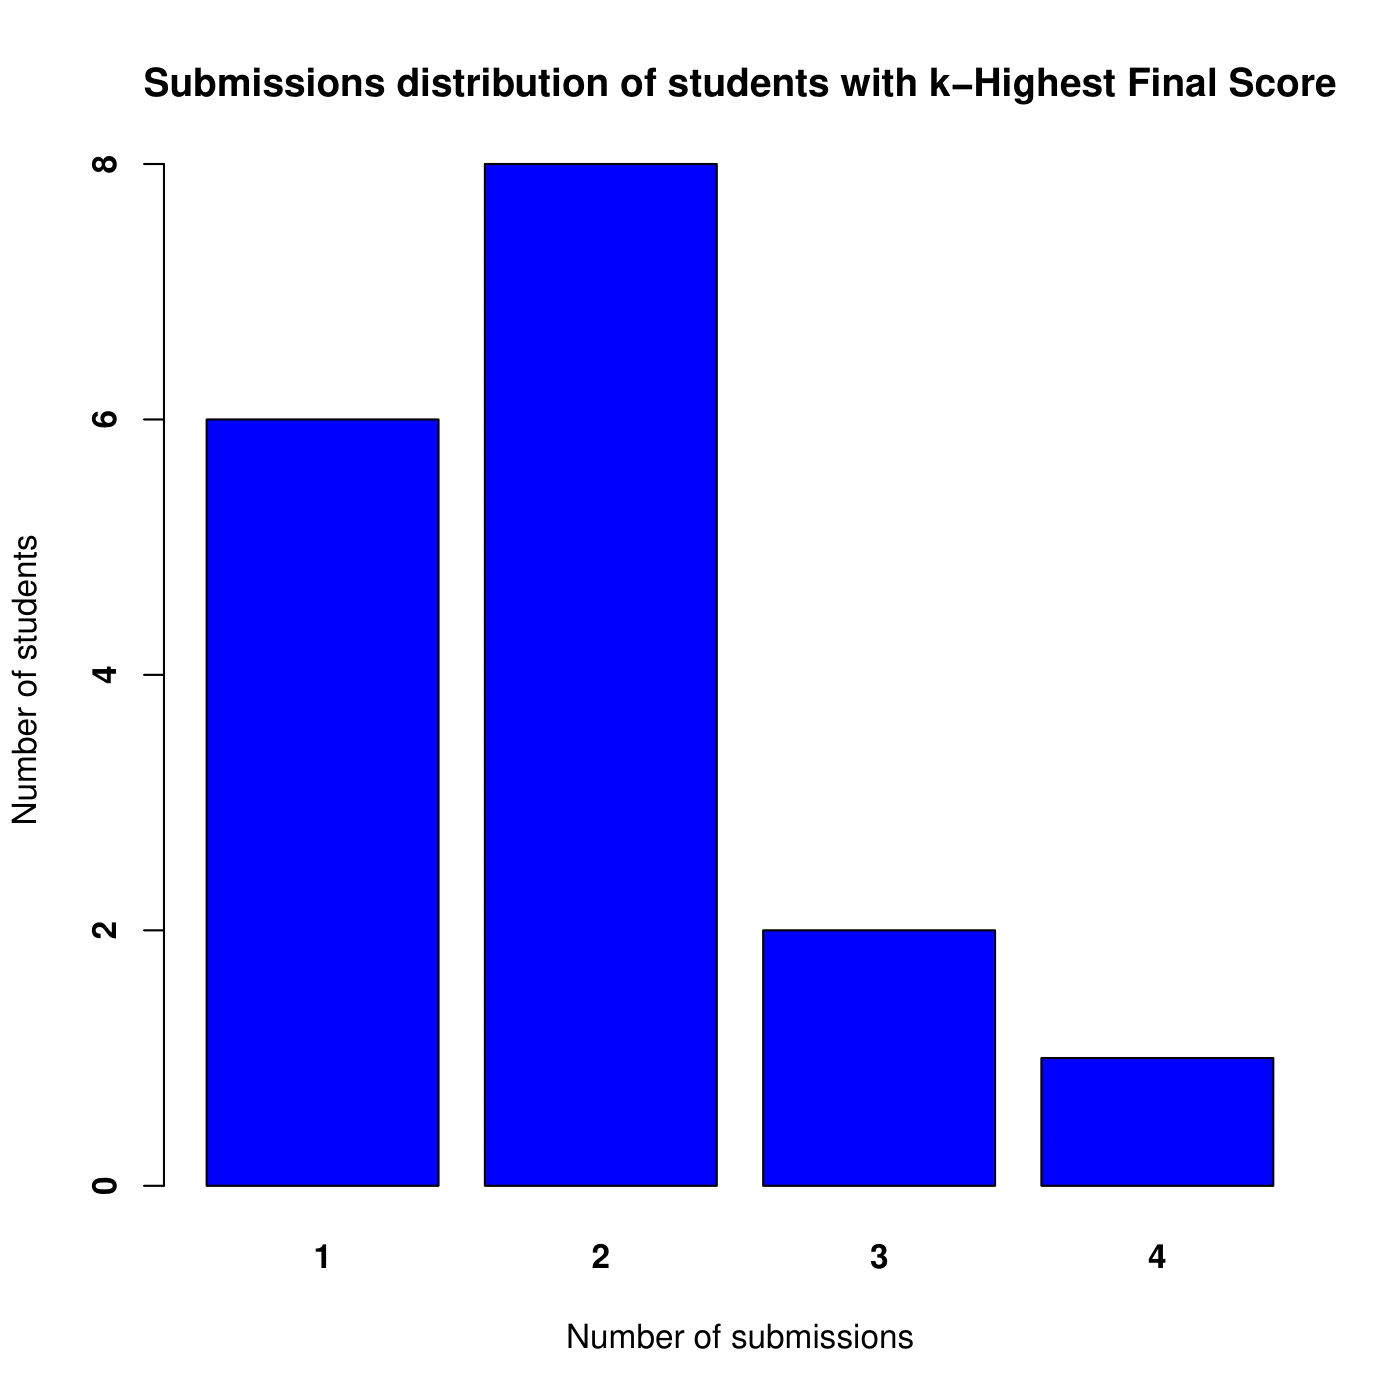
\includegraphics[width = 6.9cm]{Images/img2-7-1.png} & 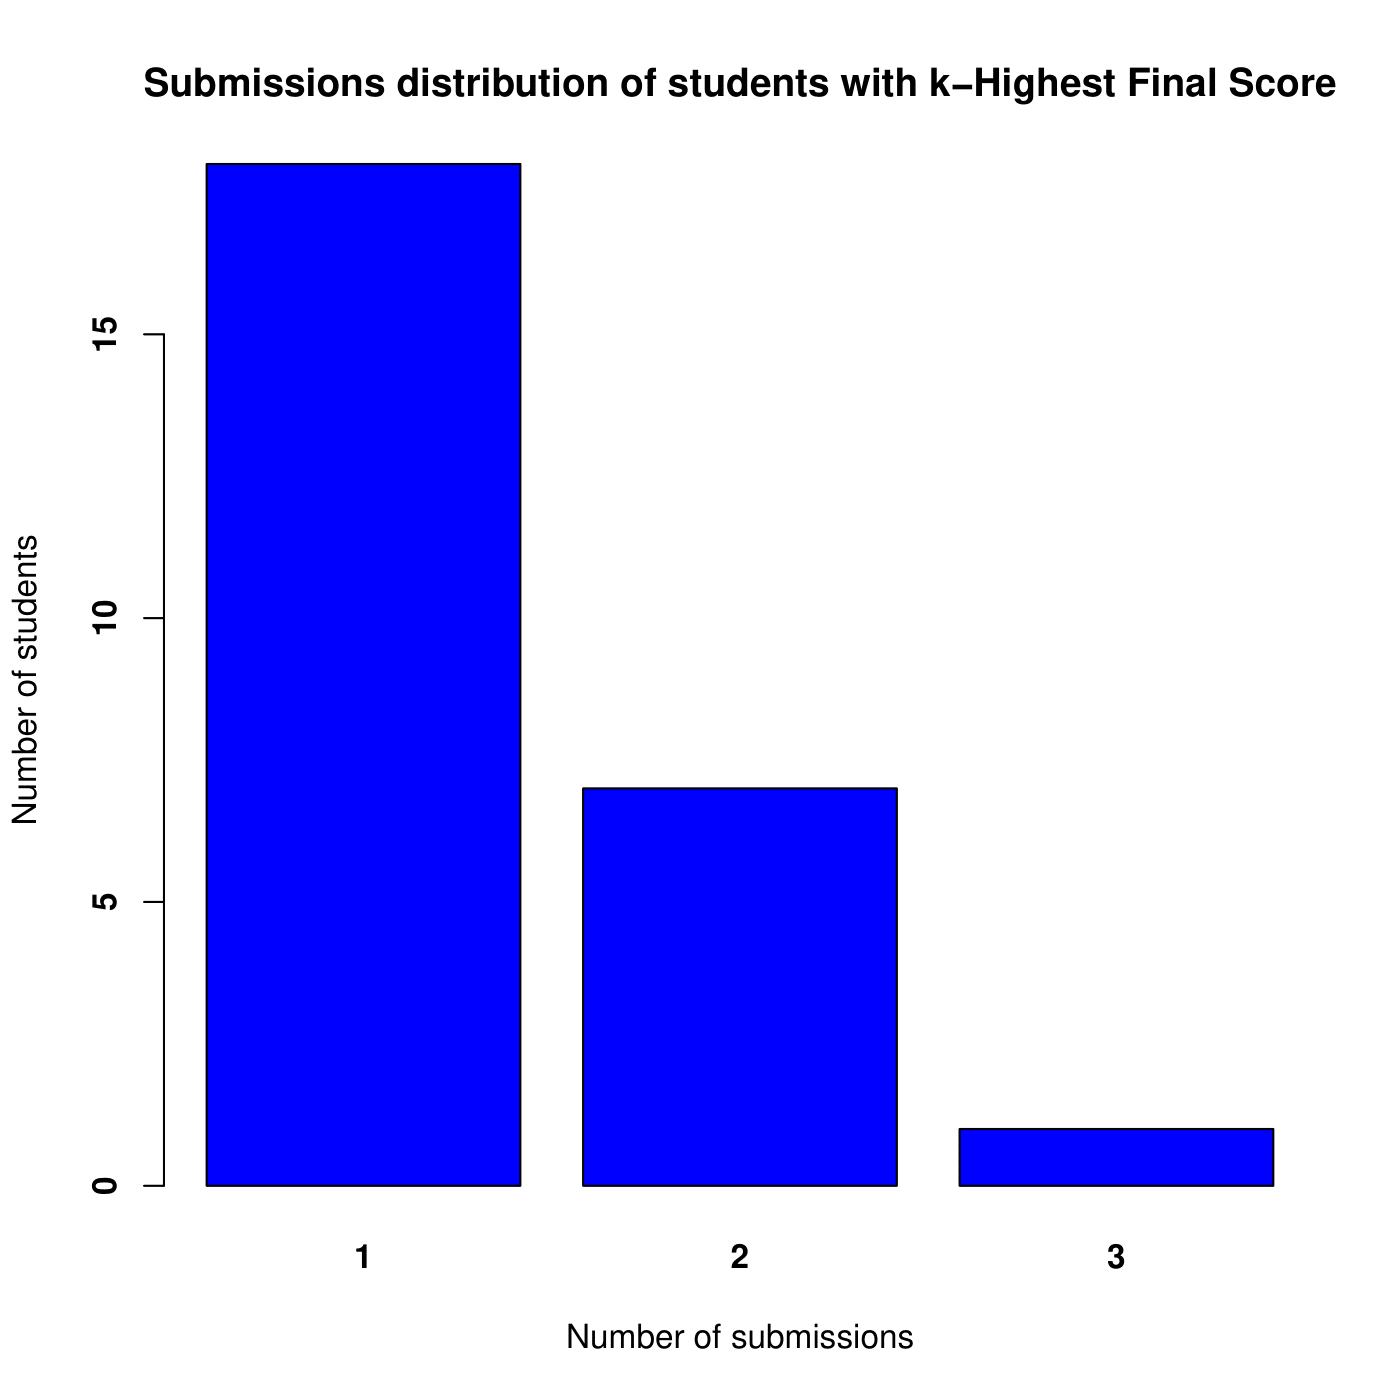
\includegraphics[width = 6.9cm]{Images/img2-7-2.png} \\
                 (1) & (2) \\
                 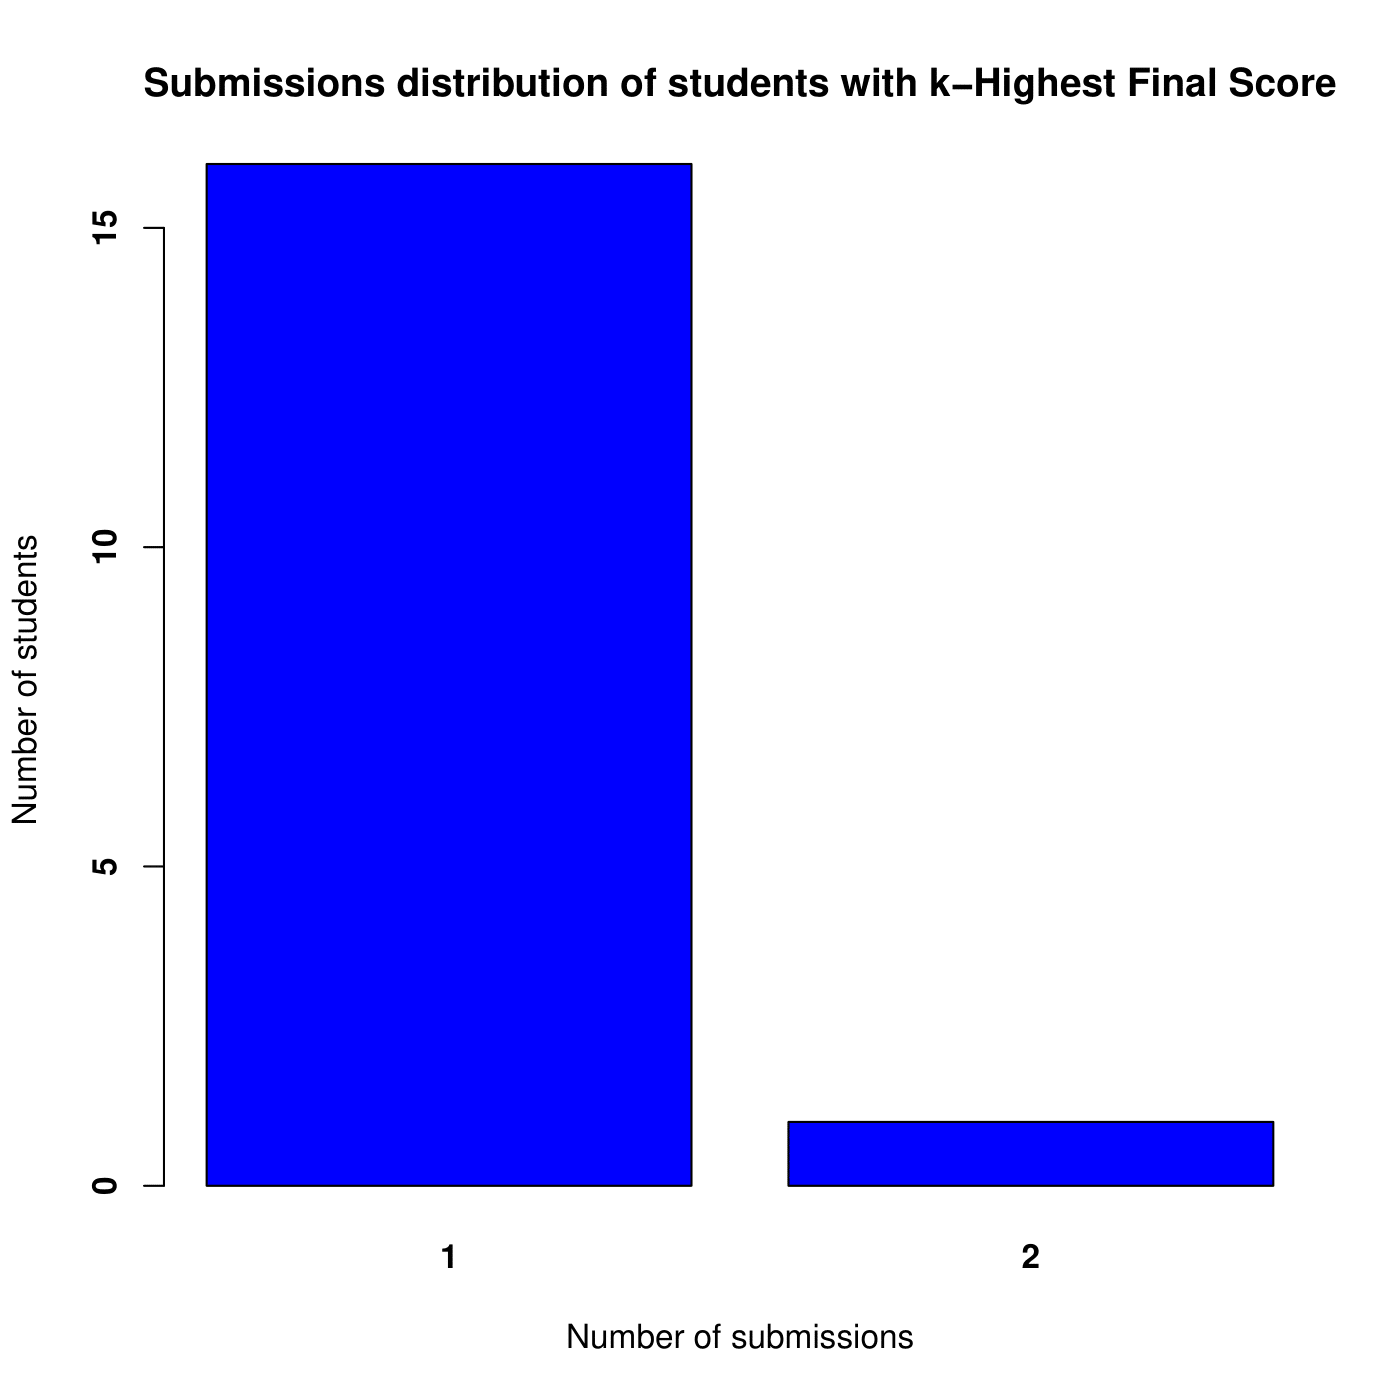
\includegraphics[width = 6.9cm]{Images/img2-7-3.png} &
                 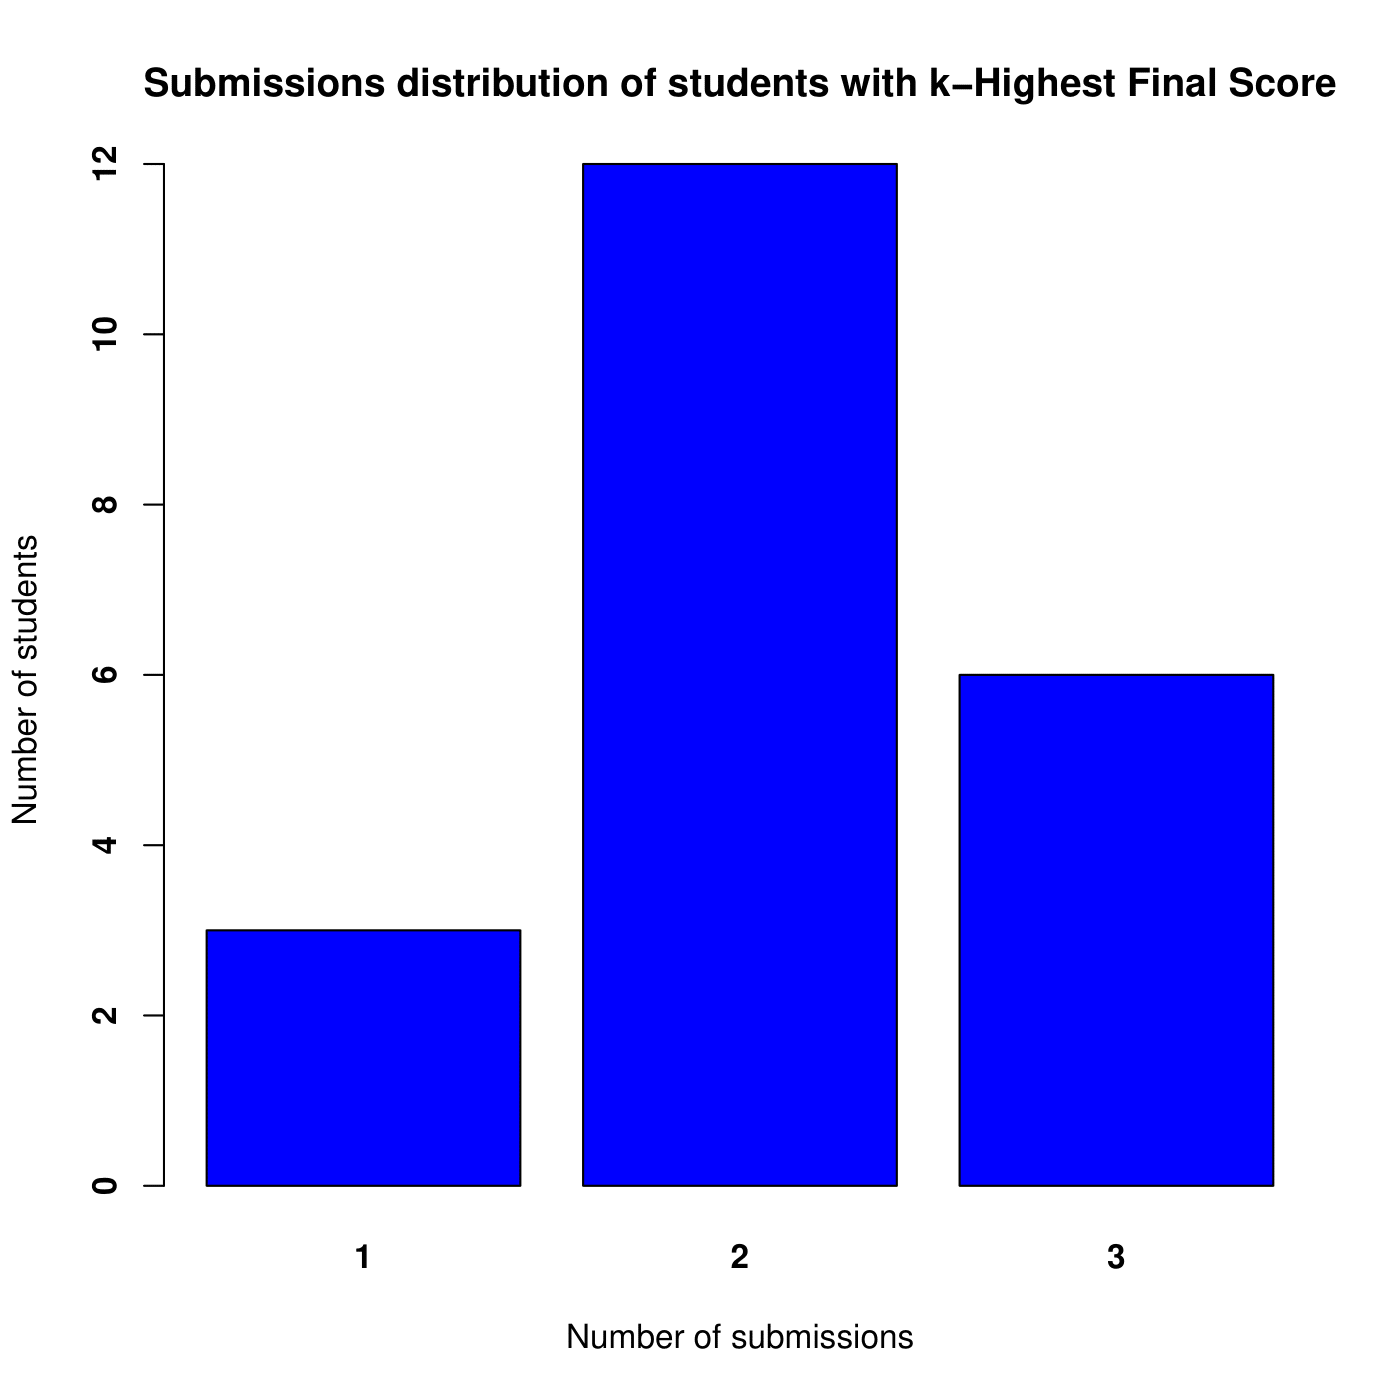
\includegraphics[width = 6.9cm]{Images/img2-7-4.png} \\
                 (3) & (4)
            \end{tabular}\\
            \textbf{Hình 2.7:} Phổ số lần nộp bài của các sinh viên với điểm tổng kết ở mức điểm cao thứ $k$\\
            \begin{tabular}{c c}
                 (1) & \texttt{"CO1007\_TV\_HK192-Quiz 1.4-điểm.xlsx"}\\
                 (2) & \texttt{"CO1007\_TV\_HK192-Quiz 1.5-điểm.xlsx"}\\
                 (3) & \texttt{"CO1007\_TV\_HK192-Quiz 3.3-điểm.xlsx"}\\
                 (4) & \texttt{"CO1007\_TV\_HK192-Quiz 4.2-điểm.xlsx"}
            \end{tabular}
        \end{center}
    \end{itemize}
\end{enumerate}


%%%%%%%%%%%%%%%%%%%%%%%%%%%%%%%%%%%%%%%%%%%%%%%%%%%%%%%%%%%%%%%%%%%%%%%%%%%%%%%%%%%%%%%%%%%%%%%%%%%%%%%%
%         ->       Bai 3
%%%%%%%%%%%%%%%%%%%%%%%%%%%%%%%%%%%%%%%%%%%%%%%%%%%%%%%%%%%%%%%%%%%%%%%%%%%%%%%%%%%%%%%%%%%%%%%%%%%%%%%%
\addcontentsline{toc}{subsubsection}{Bài 3: Nhóm câu hỏi liên quan đến số lần nộp bài}
\subsubsection*{Bài 3: Nhóm câu hỏi liên quan đến số lần nộp bài}
\begin{enumerate}[a)]
    %Cau a
    \bf\item {Xác định số lần nộp bài ít nhất}\\[6pt]
    \bf Kiến thức chuẩn bị\normalfont
    \begin{itemize}
        \item Cách giải truyền thống:
        \begin{itemize}
            \item Ta đếm số lần lặp lại của các ID để biết được số lần nộp bài tương ứng với những Mã số ID đó rồi lập thành danh sách. Từ đó ta thấy được số lần nộp bài ít nhất.
        \end{itemize}
    \end{itemize}
    \bf Hiện thực trên R\normalfont
    \begin{itemize}
        \item Ý tưởng thực hiện:
        \begin{itemize}
            \item Trước hết ta cần xử lí dữ liệu, loại bỏ các sinh viên có Mã số ID không xác định và các sinh viên chưa làm bài quiz. Dùng lệnh $subset()$ để tạo ra danh sách con của dữ liệu ban đầu với điều kiện ID không phải giá trị NA và trạng thái là "Đã hoàn thành":
            \begin{center}
                \begin{tabular}{p{13cm}}
                    \texttt{clean\_data <- subset(data, !is.na(ID) \& Status == "Done")}
                \end{tabular}
            \end{center}
            \item Dùng hàm $count()$ để lập danh sách tần số xuất hiện của các ID trong dữ liệu đã xử lí. Đó cũng chính là số lần nộp bài tương ứng.
            \begin{center}
                \begin{tabular}{p{13cm}}
                    \texttt{submission\_table <- count(clean\_data\$ID)}
                \end{tabular}
            \end{center}
            \item Dùng hàm $min()$ để tìm ra số lần nộp bài ít nhất.
            \begin{center}
                \begin{tabular}{p{13cm}}
                    \texttt{min\_num <- min(submission\_table\$freq)}
                \end{tabular}
            \end{center}
        \end{itemize}
        \item Kết quả:
        \begin{itemize}
            \item Số lần nộp bài ít nhất ứng với mỗi file:
            \begin{center}
                \begin{tabular}{l l}
                     \texttt{"CO1007\_TV\_HK192-Quiz 1.4-điểm.xlsx"} & 1 lần\\ 
                     \texttt{"CO1007\_TV\_HK192-Quiz 1.5-điểm.xlsx"} & 1 lần\\ 
                     \texttt{"CO1007\_TV\_HK192-Quiz 3.3-điểm.xlsx"} & 1 lần\\ 
                     \texttt{"CO1007\_TV\_HK192-Quiz 4.2-điểm.xlsx"} & 1 lần\\ 
                \end{tabular}
            \end{center}
        \end{itemize}
    \end{itemize}
    %Cau b
    \bf\item {Xác định danh sách các sinh viên có số lần nộp bài ít nhất} \\[6pt]
    \bf Kiến thức chuẩn bị\normalfont
    \begin{itemize}
        \item Cách giải truyền thống:
        \begin{itemize}
            \item Ta đã biết số lần nộp bài ít nhất. Từ đó ta lọc được danh sách các sinh viên có số lần nộp bài ít nhất đó từ dữ liệu.
        \end{itemize}
    \end{itemize}
    \bf Hiện thực trên R\normalfont
    \begin{itemize}
        \item Ý tưởng thực hiện:
        \begin{itemize}
            \item Để tiện cho các câu sau, ta xử lí dữ liệu một lần nữa. Vì ta chỉ cần xét điểm của lần nộp bài sau cùng nên ta loại bỏ các ID trùng lặp và chỉ giữ lại lần xuất hiện cuối cùng bằng lệnh $duplicated()$. Sau đó ta gộp danh sách số lần nộp bài của các sinh viên vào dữ liệu. Để đảm bảo chính xác, ta sắp xếp dữ liệu theo đúng thứ tự của các ID bằng lệnh $order()$ trước khi gộp.
            \begin{center}
                \begin{tabular}{p{13cm}}
                    \texttt{filtered\_data <- clean\_data[!rev(duplicated(rev(clean\_data\$ID))),]}\\
                    \texttt{arranged\_data <- filtered\_data[order(filtered\_data\$ID),]}\\
                    \texttt{arranged\_data\$submission = submission\_table\$freq}
                \end{tabular}
            \end{center}
            \item Từ dữ liệu đã được xử lí, ta lọc được danh sách các sinh viên có số lần nộp bài ít nhất tương ứng đã tìm được ở câu a bằng lệnh $subset()$. Từ danh sách này ta có được danh sách ID của các sinh viên đó.
            \begin{center}
                \begin{tabular}{p{13cm}}
                    \texttt{least\_subset <- subset(arranged\_data, submission == min\_num)}\\
                    \texttt{least\_subset\$ID}
                \end{tabular}
            \end{center}
        \end{itemize}
        \item Kết quả:
        \begin{itemize}
            \item Danh sách các sinh viên có số lần nộp bài ít nhất của mỗi file:
            \begin{center}
                \begin{tabular}{l c c c c}
                     \texttt{"CO1007\_TV\_HK192-Quiz 1.4-điểm.xlsx"} & 1812257 & 1812478 & 1813096 & 1813528 \\ & 1813681 & 1814611 & 1820028 & 1910076 \\ & 1910094 & 1910101 & 1910110 & 1910137 \\ & 1910224 & 1910238 & 1910339 & 1910346 \\ & 1910473 & 1910643 & 1910663 & 1910666 \\
                     & ...\\
                     \texttt{"CO1007\_TV\_HK192-Quiz 1.5-điểm.xlsx"} & 1812257 & 1812478 & 1813528 & 1820028 \\ & 1910076 & 1910094 & 1910137 & 1910198 \\ & 1910224 & 1910265 & 1910339 & 1910346 \\ & 1910351 & 1910473 & 1910565 & 1910643 \\ & 1910650 & 1910735 & 1910984 & 1911000\\
                     & ...\\
                     \texttt{"CO1007\_TV\_HK192-Quiz 3.3-điểm.xlsx"} & 1613010 & 1812257 & 1812478 & 1813096 \\ & 1813681 & 1814096 & 1814518 & 1820028 \\ & 1910006 & 1910032 & 1910038 & 1910060 \\ & 1910076 & 1910094 & 1910101 & 1910110 \\ & 1910113 & 1910137 & 1910202 & 1910224\\
                     & ...\\
                     \texttt{"CO1007\_TV\_HK192-Quiz 4.2-điểm.xlsx"} & 1812257 & 1910094 & 1910110 & 1910402 \\ & 1910473 & 1910663 & 1910984 & 1911015 \\ & 1911056 & 1911185 & 1911283 & 1911285 \\ & 1911565 & 1911569 & 1911594 & 1911704 \\ & 1911837 & 1911841 & 1911931 & 1912041\\
                     & ...
                \end{tabular}
            \end{center}
        \end{itemize}
    \end{itemize}
    %Cau c
    \bf\item {Xác định phổ điểm của các sinh viên có số lần nộp bài ít nhất}\\[6pt]
    \bf Kiến thức chuẩn bị\normalfont
    \begin{itemize}
        \item Cách giải truyền thống:
        \begin{itemize}
            \item Từ danh sách các sinh viên có số lần nộp bài ít nhất ở trên, ta vẽ được phổ điểm bằng cách thống kê tần số của các điểm số.
        \end{itemize}
    \end{itemize}
    \bf Hiện thực trên R\normalfont
    \begin{itemize}
        \item Ý tưởng thực hiện:
        \begin{itemize}
            \item Ta sử dụng hàm $table()$ để thống kế tần số của các điểm số, dùng hàm $barplot()$ để vẽ phổ điểm.
            \begin{center}
                \begin{tabular}{p{13cm}}
                    \texttt{barplot(table(least\_subset\$Total), xlab = "Score", ylab = "Count", col = "red", font = 2)}
                \end{tabular}
            \end{center}
        \end{itemize}
        \item Biểu đồ:
        \begin{center}
            \begin{tabular}{c c}
                 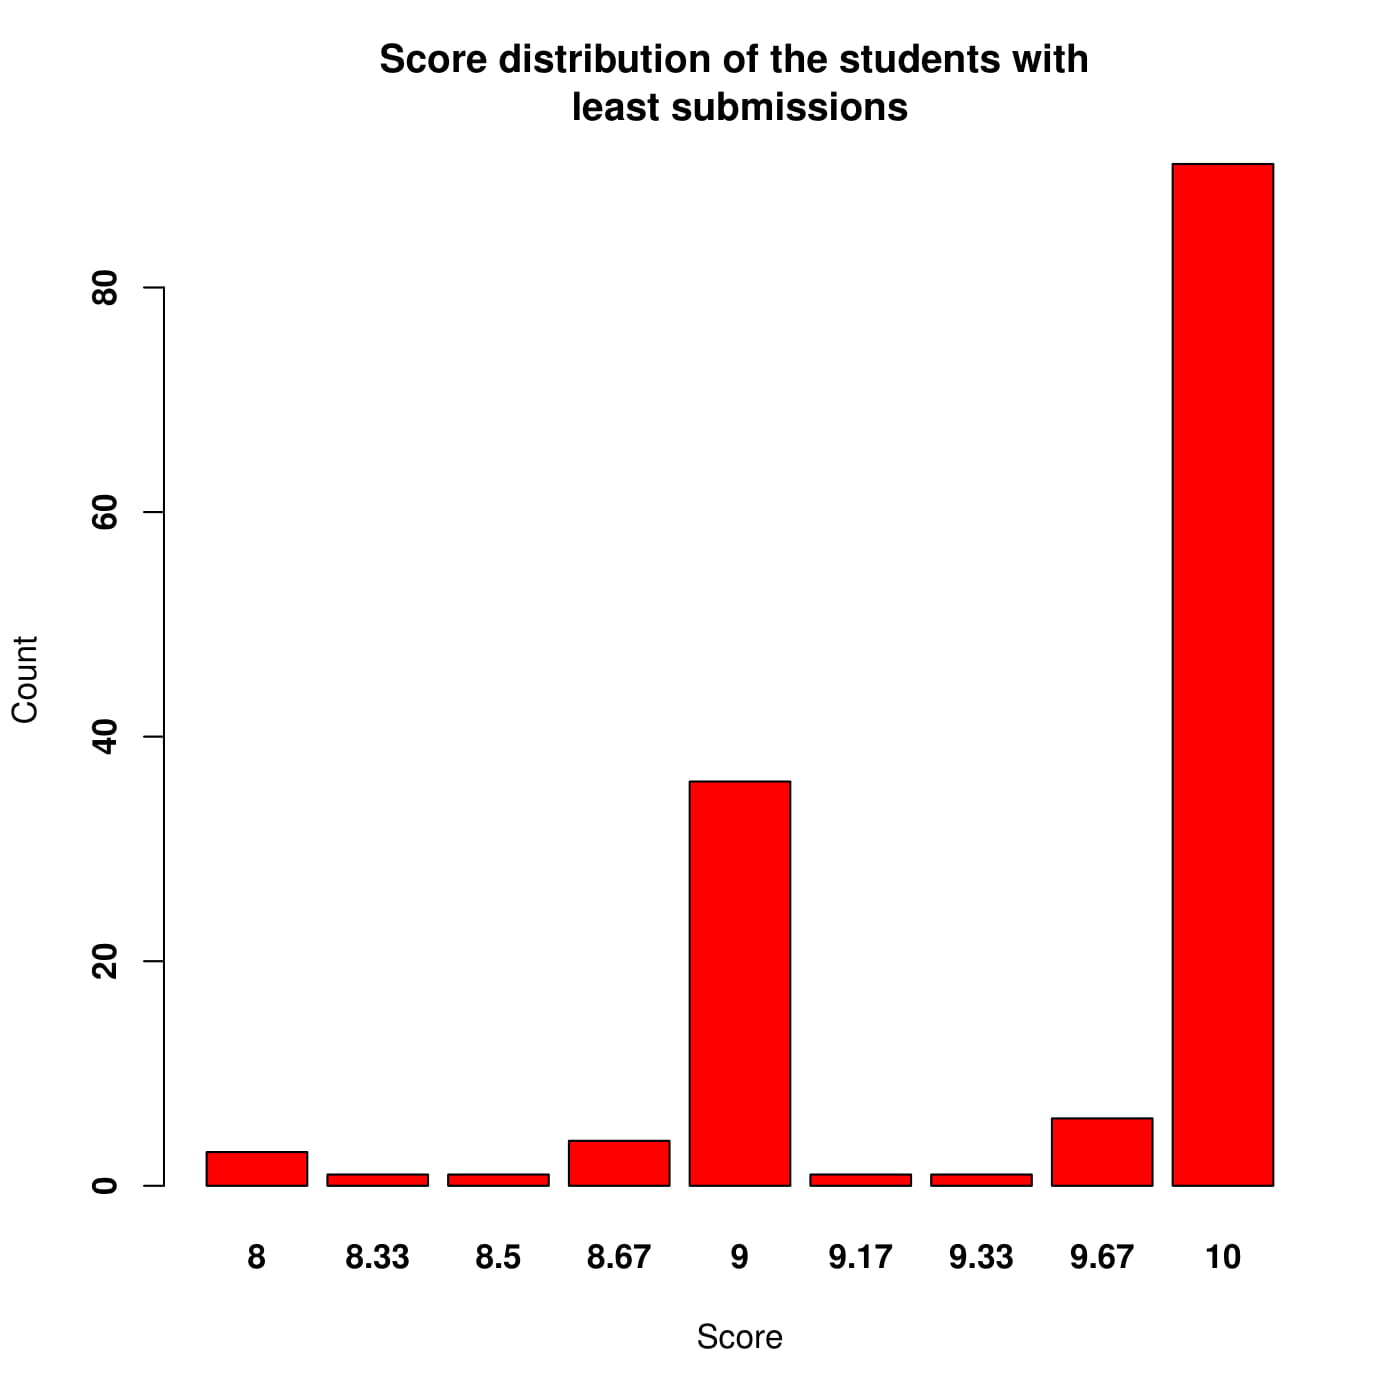
\includegraphics[width = 6.9cm]{Images/img3-1-1.jpg} & 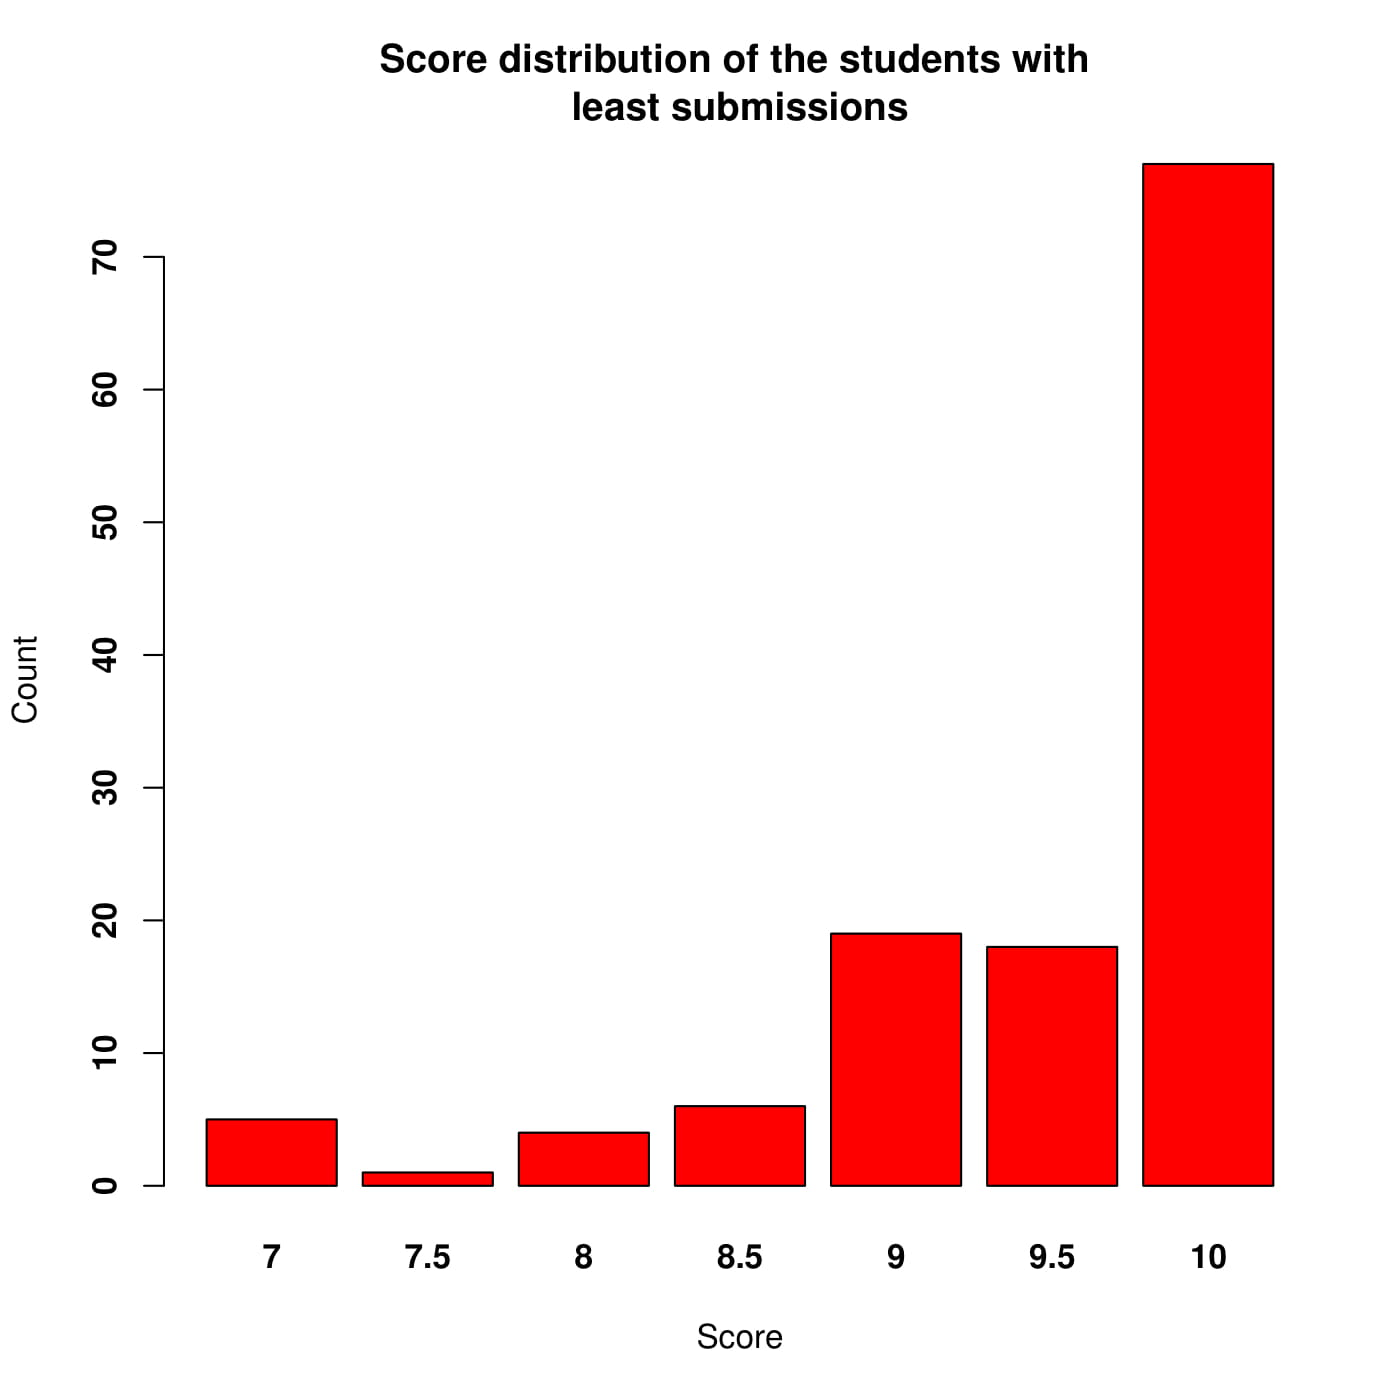
\includegraphics[width = 6.9cm]{Images/img3-1-2.jpg} \\
                 (1) & (2) \\
                 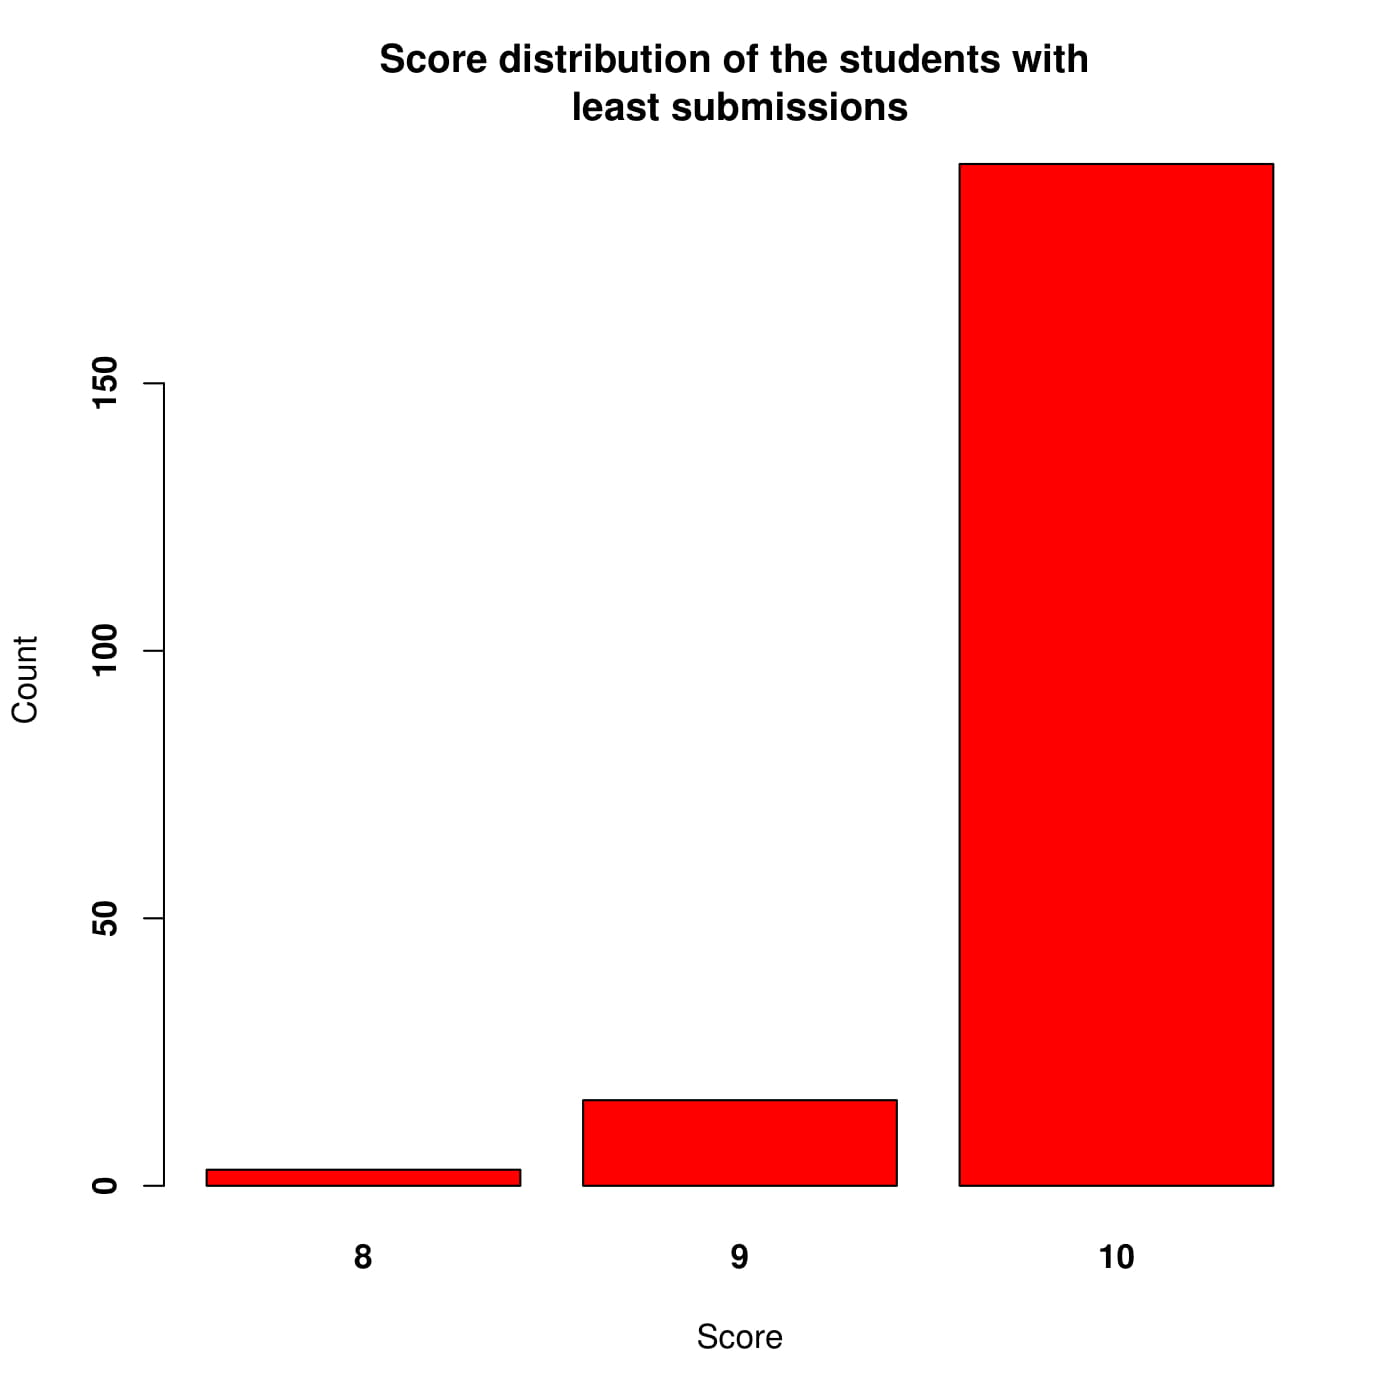
\includegraphics[width = 6.9cm]{Images/img3-1-3.png} &
                 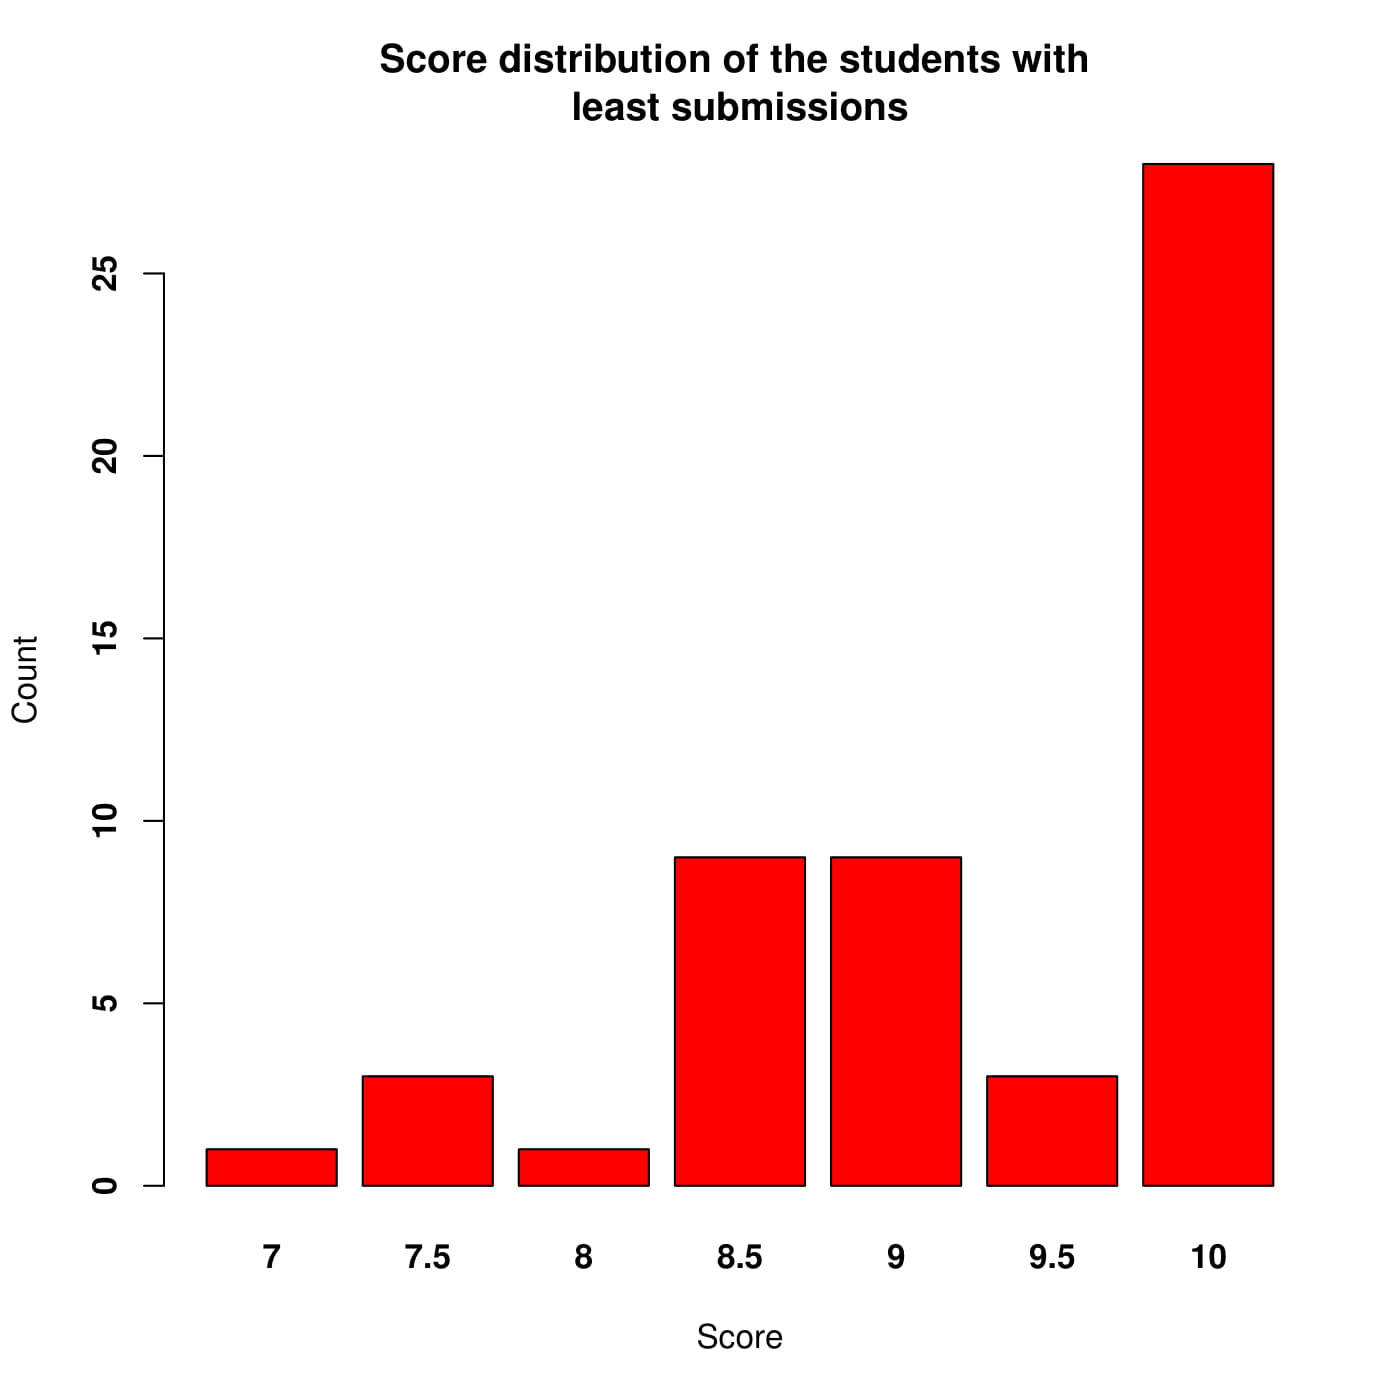
\includegraphics[width = 6.9cm]{Images/img3-1-4.png} \\
                 (3) & (4)
            \end{tabular}\\
            \textbf{Hình 3.1:} Phổ điểm của các sinh viên có số lần nộp bài ít nhất\\
            \begin{tabular}{c c}
                 (1) & \texttt{"CO1007\_TV\_HK192-Quiz 1.4-điểm.xlsx"}\\
                 (2) & \texttt{"CO1007\_TV\_HK192-Quiz 1.5-điểm.xlsx"}\\
                 (3) & \texttt{"CO1007\_TV\_HK192-Quiz 3.3-điểm.xlsx"}\\
                 (4) & \texttt{"CO1007\_TV\_HK192-Quiz 4.2-điểm.xlsx"}
            \end{tabular}
        \end{center}
    \end{itemize}
    %Cau d
    \bf\item {Xác định số lần nộp bài nhiều nhất}   \\[6pt]
    \bf Kiến thức chuẩn bị\normalfont
    \begin{itemize}
        \item Cách giải truyền thống:
        \begin{itemize}
            \item Từ danh sách tần số của các Mã số ID ở câu a, ta xác định được số lần nộp bài nhiều nhất.
        \end{itemize}
    \end{itemize}
    \bf Hiện thực trên R\normalfont
    \begin{itemize}
        \item Ý tưởng thực hiện:
        \begin{itemize}
            \item Dùng hàm $max()$ để tìm ra số lần nộp bài nhiều nhất.
            \begin{center}
                \begin{tabular}{p{13cm}}
                    \texttt{max\_num <- max(submission\_table\$freq)}
                \end{tabular}
            \end{center}
        \end{itemize}
        \item Kết quả:
        \begin{itemize}
            \item Số lần nộp bài nhiều nhất ứng với mỗi file:
            \begin{center}
                \begin{tabular}{l l}
                     \texttt{"CO1007\_TV\_HK192-Quiz 1.4-điểm.xlsx"} & 5 lần\\ 
                     \texttt{"CO1007\_TV\_HK192-Quiz 1.5-điểm.xlsx"} & 5 lần\\ 
                     \texttt{"CO1007\_TV\_HK192-Quiz 3.3-điểm.xlsx"} & 3 lần\\ 
                     \texttt{"CO1007\_TV\_HK192-Quiz 4.2-điểm.xlsx"} & 3 lần\\ 
                \end{tabular}
            \end{center}
        \end{itemize}
    \end{itemize}
    %Cau e
    \bf\item {Xác định các sinh viên có số lần nộp bài nhiều nhất}\\[6pt]
    \bf Kiến thức chuẩn bị\normalfont
    \begin{itemize}
        \item Cách giải truyền thống:
        \begin{itemize}
            \item Ta đã biết số lần nộp bài nhiều nhất. Từ đó ta lọc được danh sách các sinh viên có số lần nộp bài nhiều nhất đó từ dữ liệu.
        \end{itemize}
    \end{itemize}
    \bf Hiện thực trên R\normalfont
    \begin{itemize}
        \item Ý tưởng thực hiện:
        \begin{itemize}
            \item Từ dữ liệu đã được xử lí, ta lọc được danh sách các sinh viên có số lần nộp bài nhiều nhất tương ứng đã tìm được ở câu a bằng lệnh $subset()$. Từ danh sách này ta có được danh sách ID của các sinh viên đó.
            \begin{center}
                \begin{tabular}{p{13cm}}
                    \texttt{most\_subset <- subset(arranged\_data, submission == max\_num)}\\
                    \texttt{most\_subset\$ID}
                \end{tabular}
            \end{center}
        \end{itemize}
        \item Kết quả:
        \begin{itemize}
            \item Danh sách các sinh viên có số lần nộp bài cao nhất của mỗi file:
            \begin{center}
                \begin{tabular}{l c c c c}
                     \texttt{"CO1007\_TV\_HK192-Quiz 1.4-điểm.xlsx"} & 1910038 & 1913756\\
                     \texttt{"CO1007\_TV\_HK192-Quiz 1.5-điểm.xlsx"} & 1912817 & 1913467 & 1914768 & 1915268\\
                     \texttt{"CO1007\_TV\_HK192-Quiz 3.3-điểm.xlsx"} & 1913045 & 1915520 & 1927007\\
                     \texttt{"CO1007\_TV\_HK192-Quiz 4.2-điểm.xlsx"} & 1910032 & 1910060 & 1910666 & 1911000 \\ & 1911136 & 1912056 & 1912539 & 1912676 \\ & 1913045 & 1913306 & 1913355 & 1913467 \\ & 1913566 & 1913775 & 1913918 & 1914003 \\ & 1914011 & 1914093 & 1914659 & 1914713\\
                     & ...
                \end{tabular}
            \end{center}
        \end{itemize}
    \end{itemize}
    %Cau f
    \bf\item {Xác định phổ điểm của các sinh viên có số lần nộp bài nhiều nhất}\\[6pt]
    \bf Kiến thức chuẩn bị\normalfont
    \begin{itemize}
        \item Cách giải truyền thống:
        \begin{itemize}
            \item Từ danh sách các sinh viên có số lần nộp bài nhiều nhất ở trên, ta vẽ được phổ điểm bằng cách thống kê tần số của các điểm số.
        \end{itemize}
    \end{itemize}
    \bf Hiện thực trên R\normalfont
    \begin{itemize}
        \item Ý tưởng thực hiện:
        \begin{itemize}
            \item Ta sử dụng hàm $table()$ để thống kế tần số của các điểm số, dùng hàm $barplot()$ để vẽ phổ điểm.
            \begin{center}
                \begin{tabular}{p{13cm}}
                    \texttt{barplot(table(least\_subset\$Total), xlab = "Score", ylab = "Count", col = "red", font = 2)}
                \end{tabular}
            \end{center}
        \end{itemize}
        \item Biểu đồ:\\
        \begin{center}
            \begin{tabular}{c c}
                 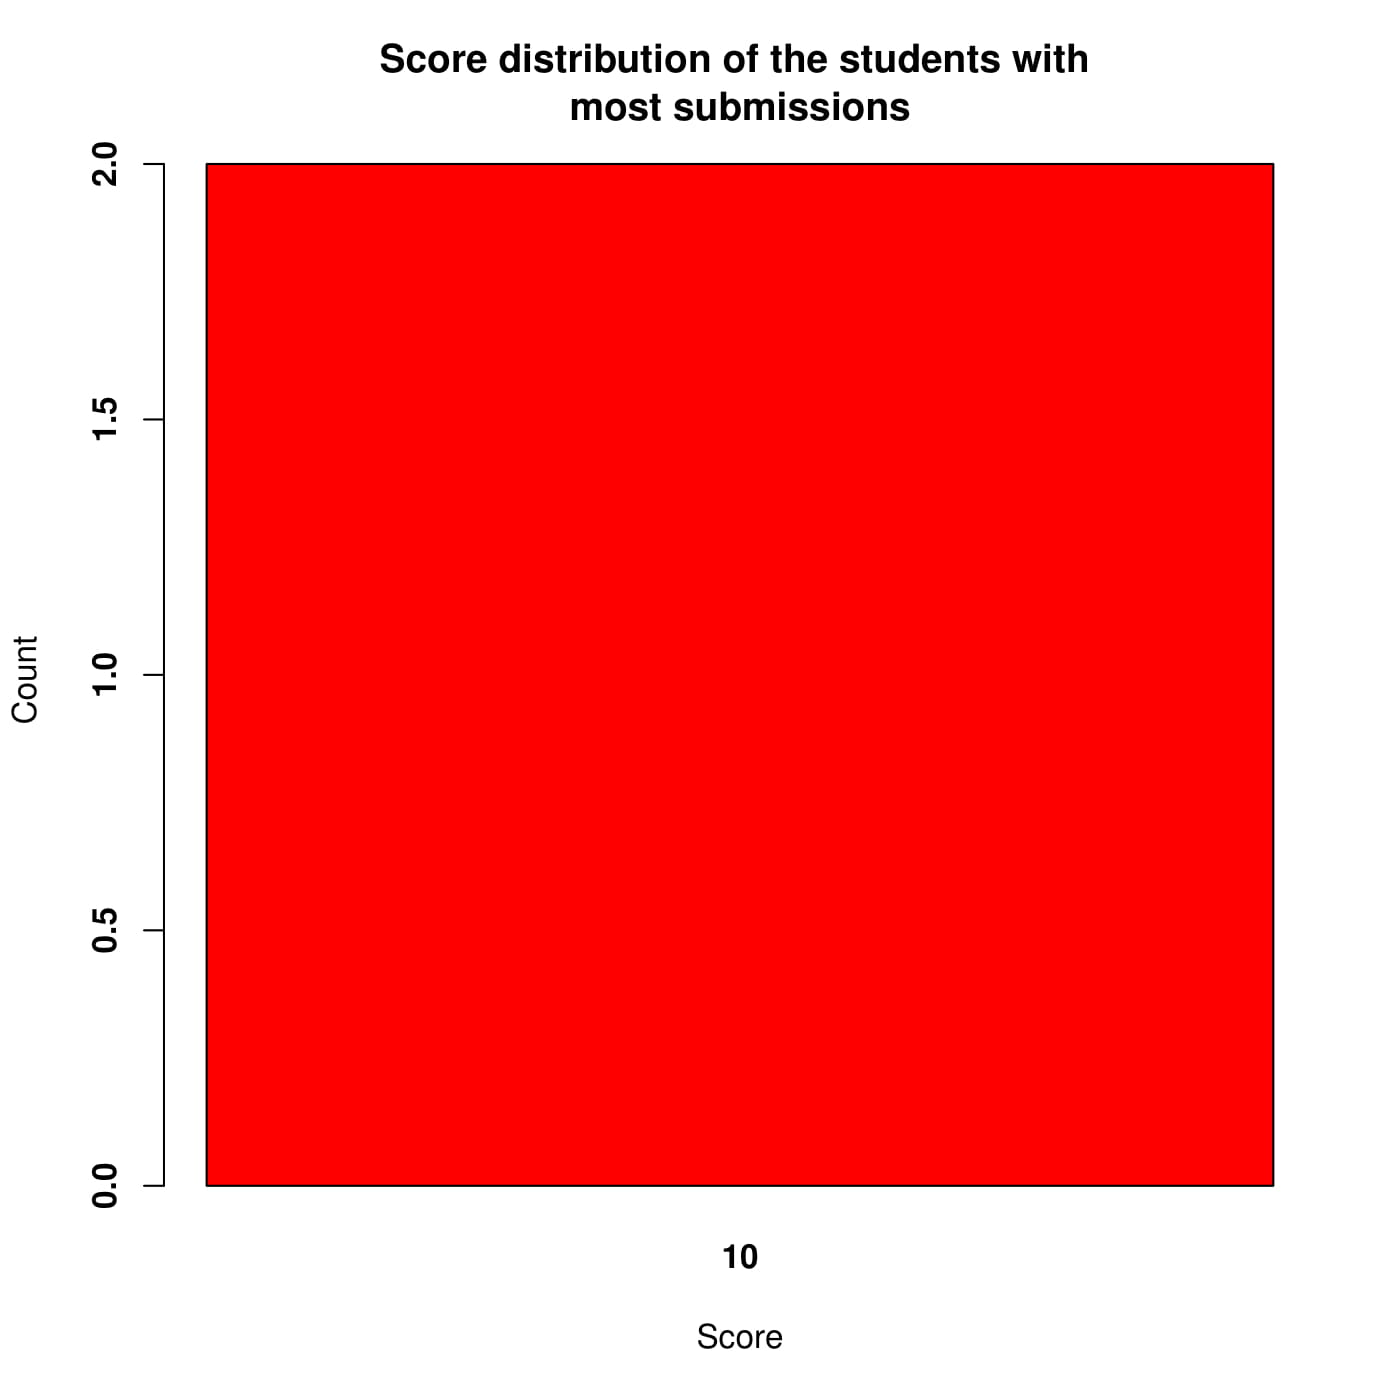
\includegraphics[width = 6.9cm]{Images/img3-2-1.png} & 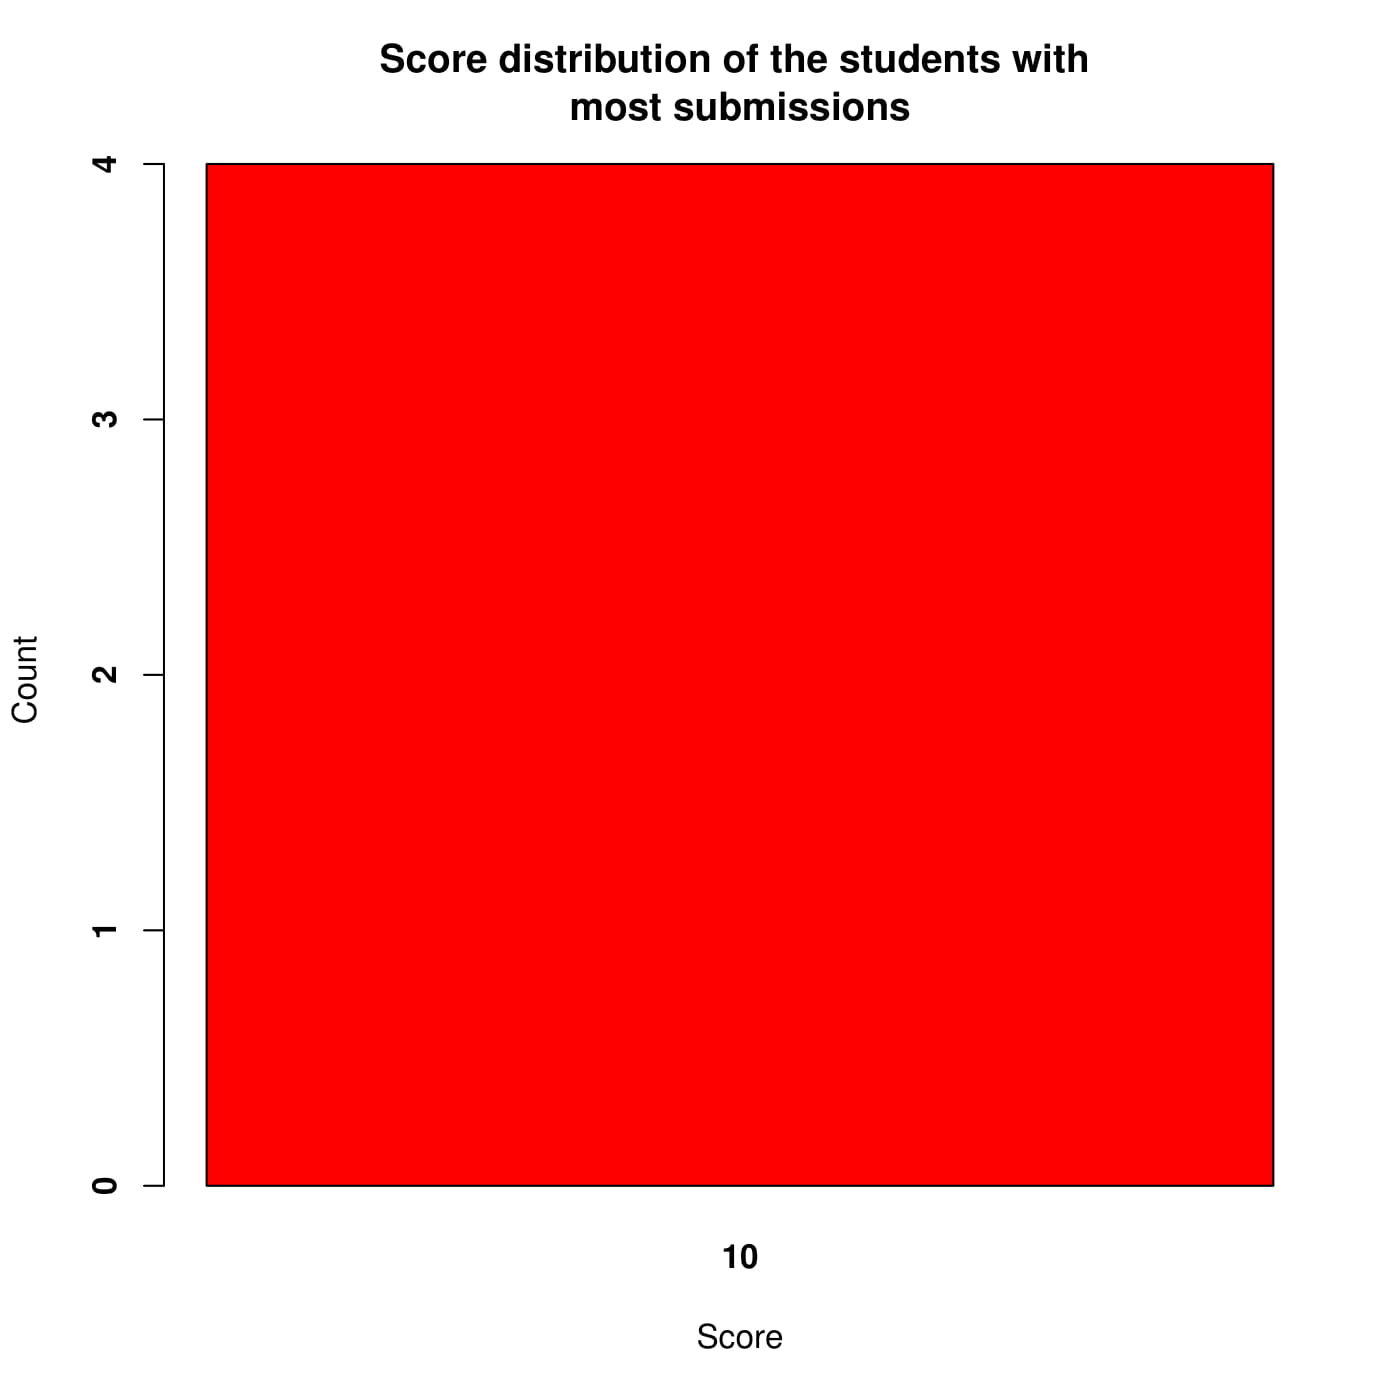
\includegraphics[width = 6.9cm]{Images/img3-2-2.png} \\
                 (1) & (2) \\
                 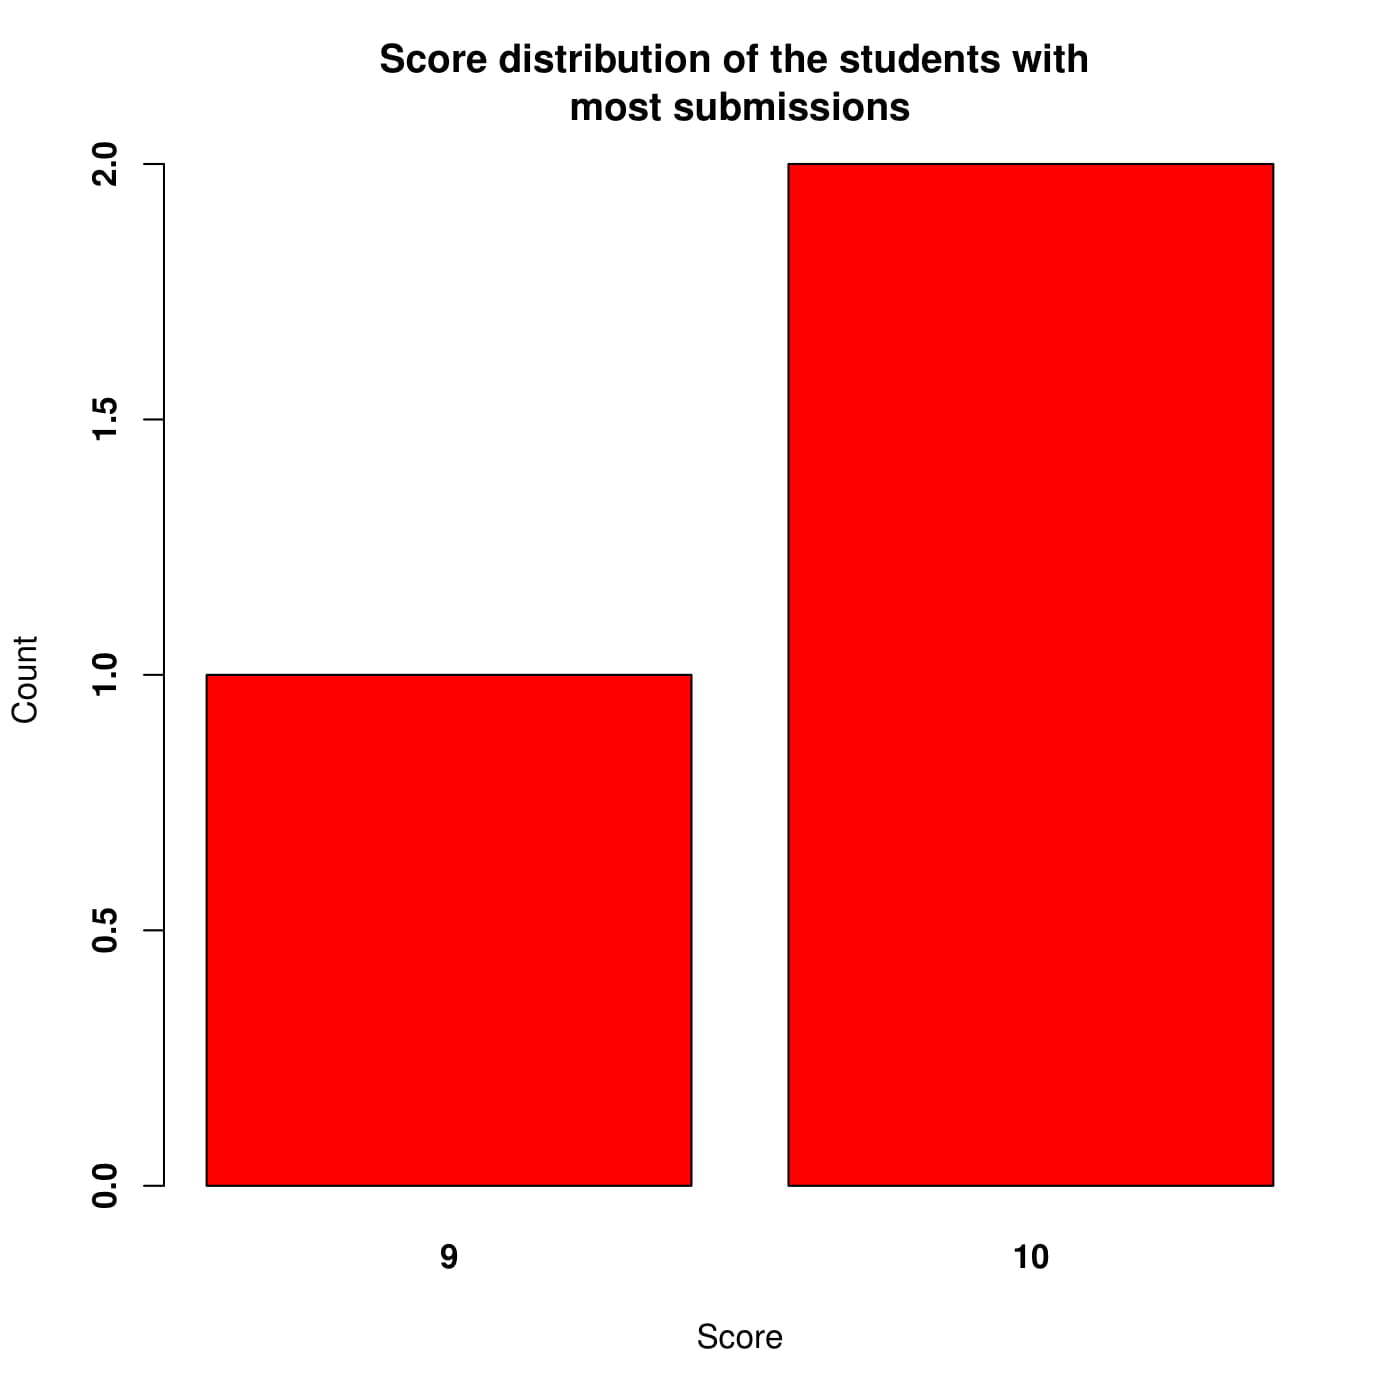
\includegraphics[width = 6.9cm]{Images/img3-2-3.png} &
                 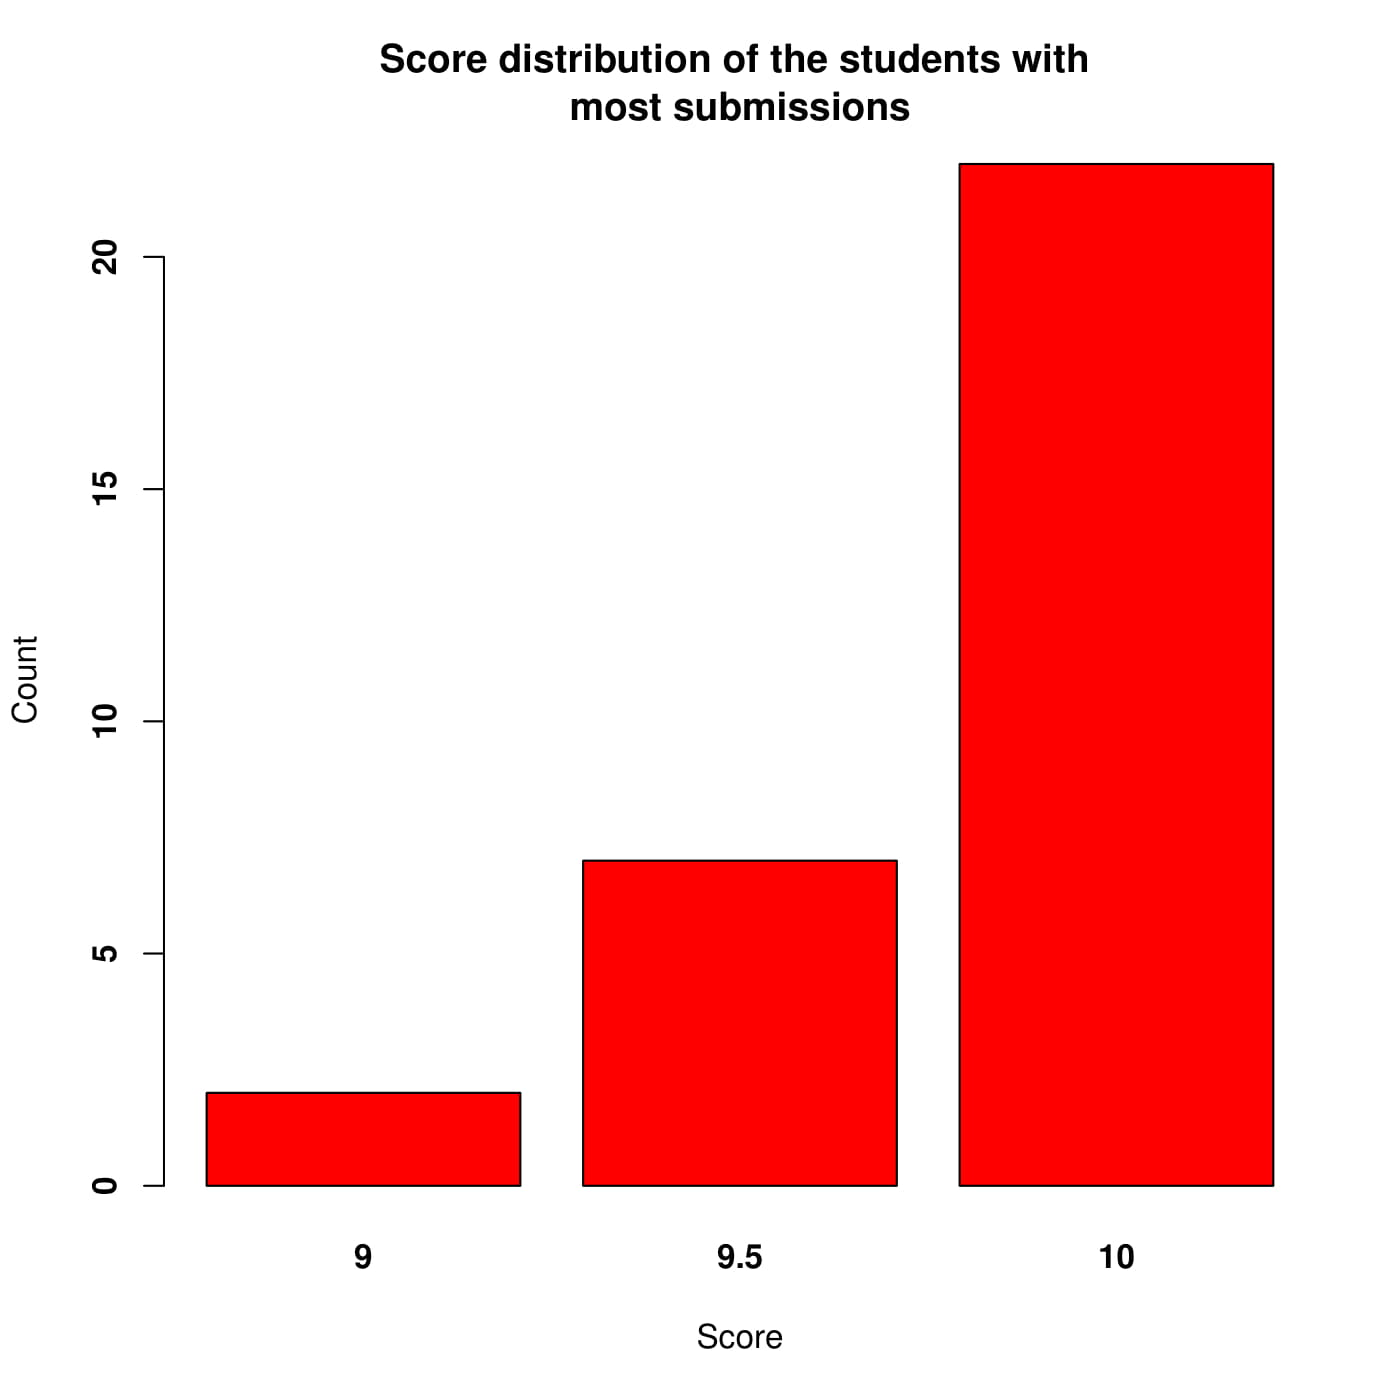
\includegraphics[width = 6.9cm]{Images/img3-2-4.png} \\
                 (3) & (4)
            \end{tabular}\\
            \textbf{Hình 3.2:} Phổ điểm của các sinh viên có số lần nộp bài nhiều nhất\\
            \begin{tabular}{c c}
                 (1) & \texttt{"CO1007\_TV\_HK192-Quiz 1.4-điểm.xlsx"}\\
                 (2) & \texttt{"CO1007\_TV\_HK192-Quiz 1.5-điểm.xlsx"}\\
                 (3) & \texttt{"CO1007\_TV\_HK192-Quiz 3.3-điểm.xlsx"}\\
                 (4) & \texttt{"CO1007\_TV\_HK192-Quiz 4.2-điểm.xlsx"}
            \end{tabular}
        \end{center}
    \end{itemize}
    %Cau g
    \bf\item Xác định số lần nộp bài trung bình của của các sinh viên \\[6pt]
    \bf Kiến thức chuẩn bị\normalfont
    \begin{itemize}
        \item Cách giải truyền thống:
        \begin{itemize}
            \item Từ danh sách tần số của các Mã số ID ở câu $a$, ta xác định được số lần nộp bài trung bình.
            \item Số lần nộp bài trung bình tính bởi:
            \begin{center}
                $\overline{x} = \frac{\sum\limits_{i = 1}^n x_i}{n}$
            \end{center}
            \begin{tabular}{p{13cm}}
                \begin{tabular}{l l}
                     trong đó: & $x_i$ là số lần nộp bài của sinh viên thứ $i$\\
                     & $n$ là tổng số sinh viên
                \end{tabular}
            \end{tabular}
        \end{itemize}
    \end{itemize}
    \bf Hiện thực trên R\normalfont
    \begin{itemize}
        \item Ý tưởng thực hiện:
        \begin{itemize}
            \item Dùng hàm $avg()$ để tìm ra số lần nộp bài trung bình, hàm $round()$ để làm tròn số.
        \end{itemize}
        \item Kết quả:
        \begin{itemize}
            \item Số lần nộp bài trung bình ứng với mỗi file:
            \begin{center}
                \begin{tabular}{l l}
                     \texttt{"CO1007\_TV\_HK192-Quiz 1.4-điểm.xlsx"} & 2 lần\\ 
                     \texttt{"CO1007\_TV\_HK192-Quiz 1.5-điểm.xlsx"} & 2 lần\\ 
                     \texttt{"CO1007\_TV\_HK192-Quiz 3.3-điểm.xlsx"} & 1 lần\\ 
                     \texttt{"CO1007\_TV\_HK192-Quiz 4.2-điểm.xlsx"} & 2 lần\\ 
                \end{tabular}
            \end{center}
        \end{itemize}
    \end{itemize}
    %Cau h
    \bf\item Xác định số lượng sinh viên có số lần nộp trung bình \\[6pt]
    \bf Kiến thức chuẩn bị\normalfont
    \begin{itemize}
        \item Cách giải truyền thống:
        \begin{itemize}
            \item Ta đã biết số lần nộp bài trung bình. Từ đó ta có thể đếm được số lượng sinh viên có số lần nộp bài trung bình từ dữ liệu.
        \end{itemize}
    \end{itemize}
    \bf Hiện thực trên R\normalfont
    \begin{itemize}
        \item Ý tưởng thực hiện:
        \begin{itemize}
            \item Từ dữ liệu đã được xử lí, ta lọc được danh sách các sinh viên có số lần nộp bài trung bình tương ứng đã tìm được bằng lệnh $subset()$. Đếm số ID trong danh sách này bằng lệnh $length()$ ta có được số lượng sinh viên có số lần nộp bài trung bình.
            \begin{center}
                \begin{tabular}{p{13cm}}
                    \texttt{avg\_subset <- subset(arranged\_data, submission == avg\_num)}\\
                    \texttt{length(avg\_subset\$ID)}
                \end{tabular}
            \end{center}    
        \end{itemize}
        \item Kết quả:
        \begin{itemize}
            \item Số lượng sinh viên có số lần nộp bài trung bình ứng với mỗi file
            \begin{center}
                \begin{tabular}{l l}
                     \texttt{"CO1007\_TV\_HK192-Quiz 1.4-điểm.xlsx"} & 160 sinh viên\\ 
                     \texttt{"CO1007\_TV\_HK192-Quiz 1.5-điểm.xlsx"} & 163 sinh viên\\ 
                     \texttt{"CO1007\_TV\_HK192-Quiz 3.3-điểm.xlsx"} & 210 sinh viên\\ 
                     \texttt{"CO1007\_TV\_HK192-Quiz 4.2-điểm.xlsx"} & 175 sinh viên\\ 
                \end{tabular}
            \end{center}        
        \end{itemize}
    \end{itemize}
    %Cau i
    \bf\item {Xác định phổ theo điểm số của các sinh viên có lần nộp bài trung bình}\\[6pt]
    \bf Kiến thức chuẩn bị\normalfont
    \begin{itemize}
        \item Cách giải truyền thống:
        \begin{itemize}
            \item Từ danh sách các sinh viên có số lần nộp bài trung bình ở trên, ta vẽ được phổ điểm bằng cách thống kê tần số của các điểm số.
        \end{itemize}
    \end{itemize}
    \bf Hiện thực trên R\normalfont
    \begin{itemize}
        \item Ý tưởng thực hiện:
        \begin{itemize}
            \item Ta sử dụng hàm $table()$ để thống kế tần số của các điểm số, dùng hàm $barplot()$ để vẽ phổ điểm.
            \begin{center}
                \begin{tabular}{p{13cm}}
                    \texttt{barplot(table(avg\_subset\$Total), xlab = "Score", ylab = "Count", col = "red", font = 2)}
                \end{tabular}
            \end{center}
        \end{itemize}
        \item Biểu đồ:\\
        \begin{center}
            \begin{tabular}{c c}
                 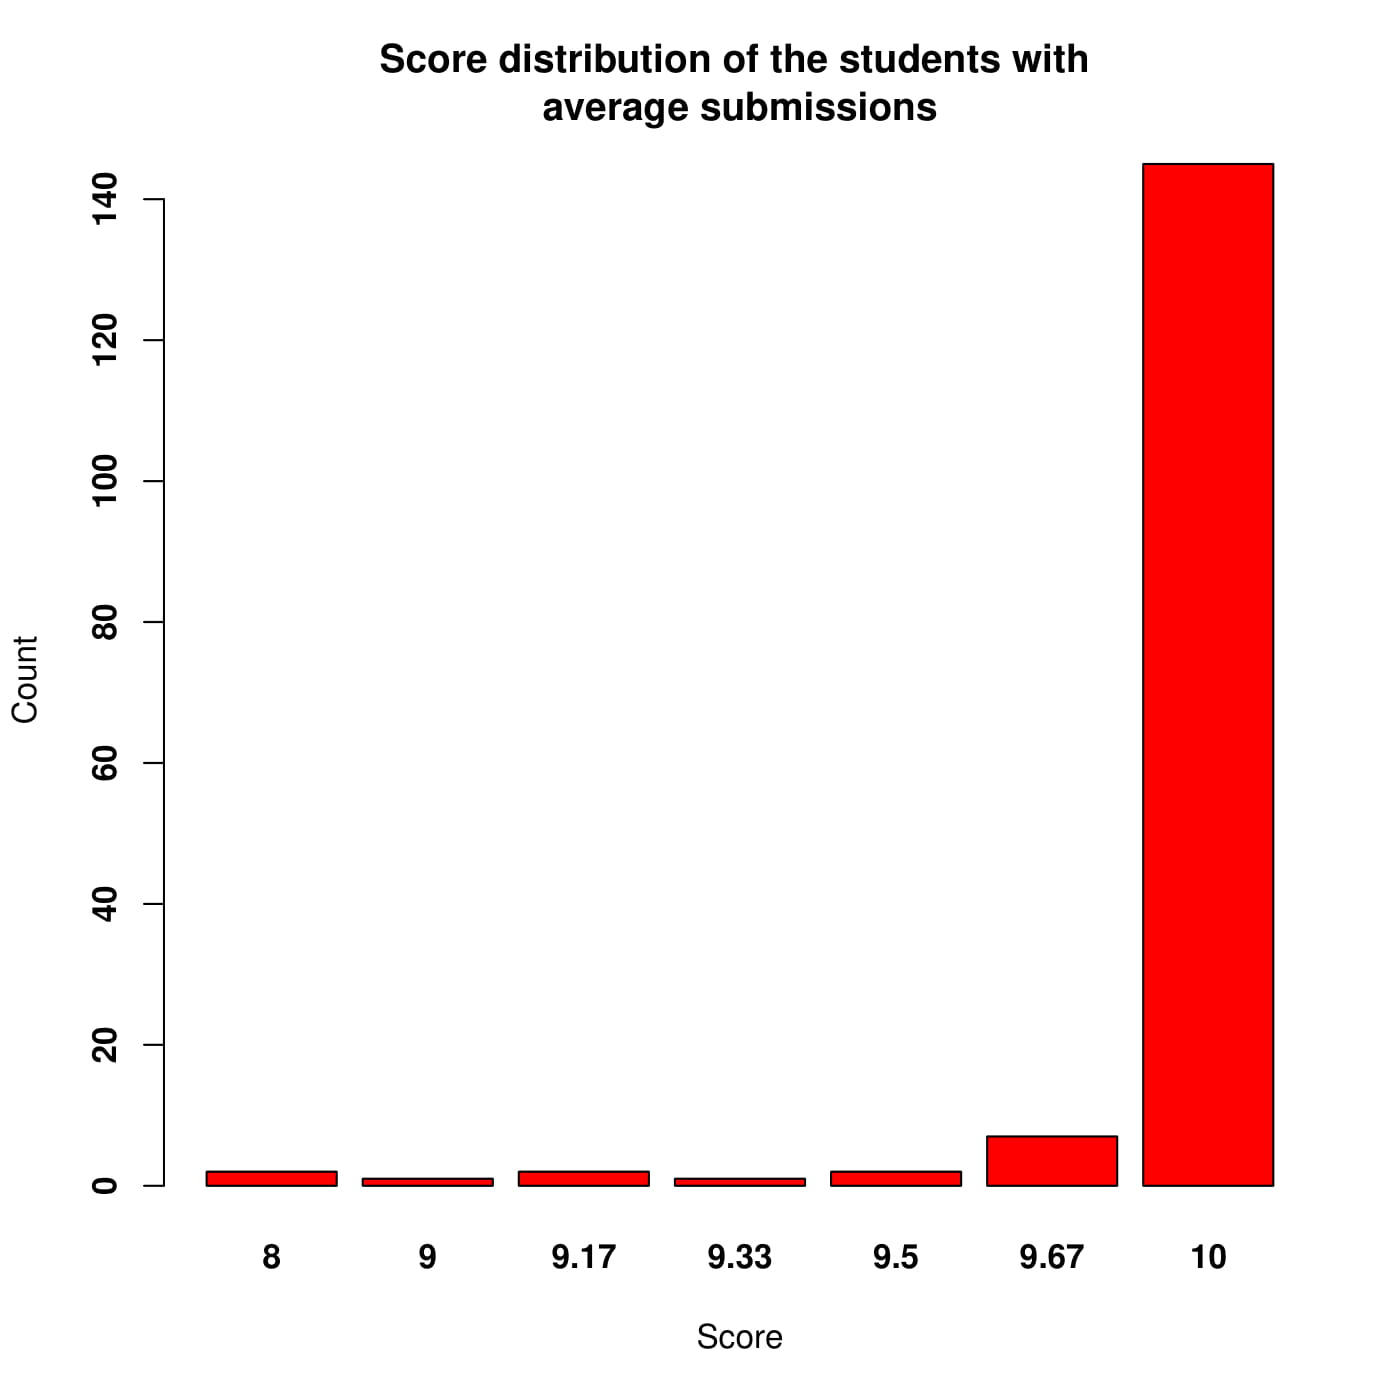
\includegraphics[width = 6.9cm]{Images/img3-3-1.png} & 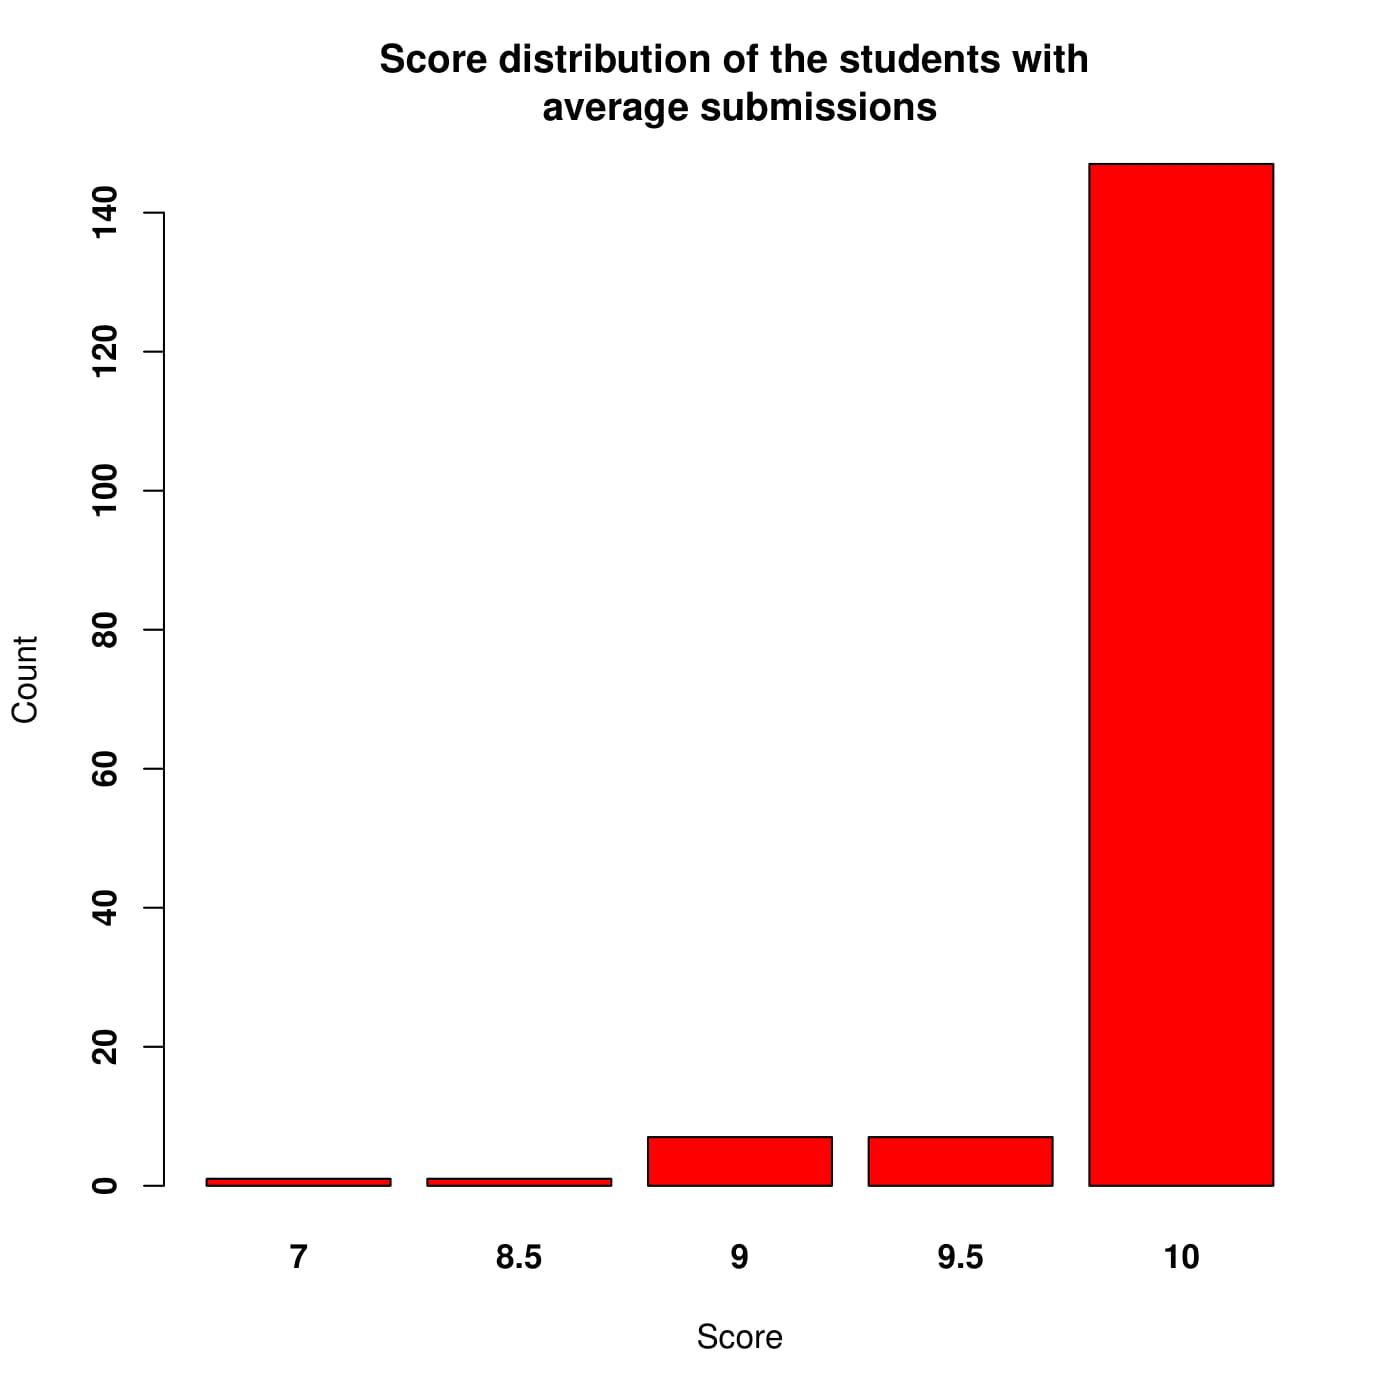
\includegraphics[width = 6.9cm]{Images/img3-3-2.png} \\
                 (1) & (2) \\
                 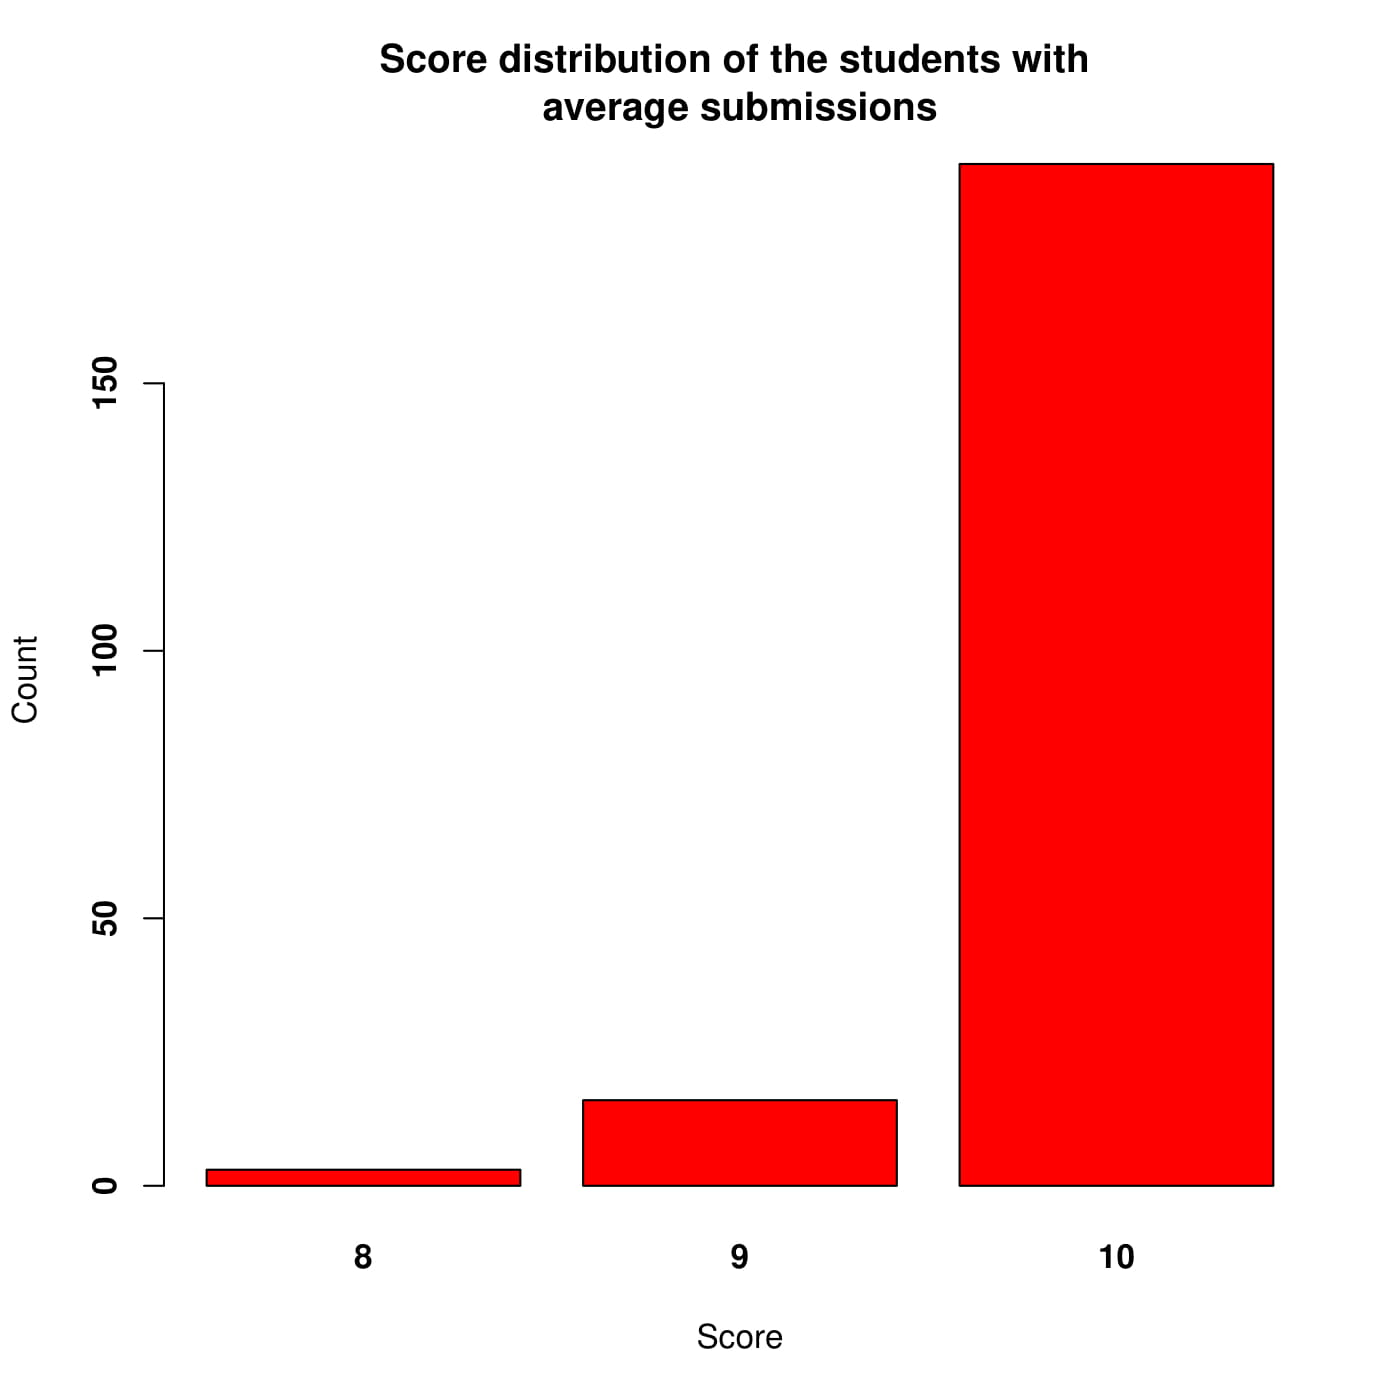
\includegraphics[width = 6.9cm]{Images/img3-3-3.png} &
                 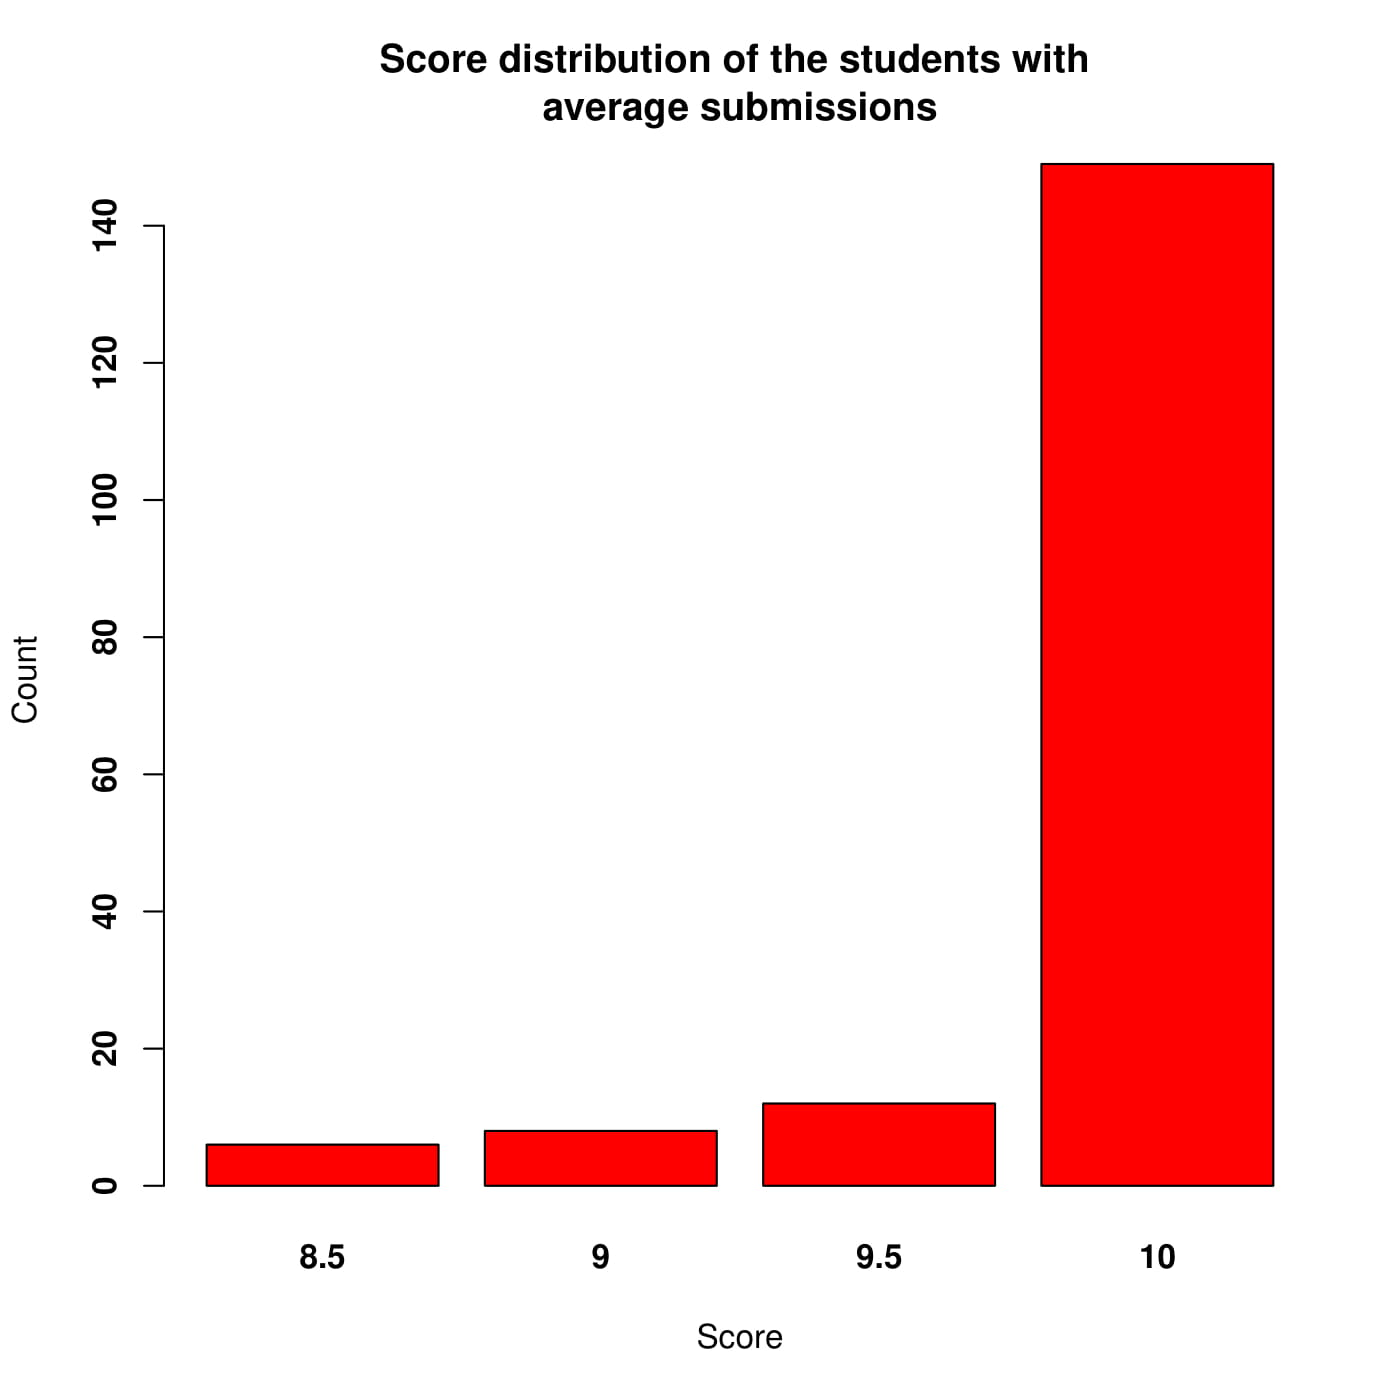
\includegraphics[width = 6.9cm]{Images/img3-3-4.png} \\
                 (3) & (4)
            \end{tabular}\\
            \textbf{Hình 3.3:} Phổ điểm của các sinh viên có số lần nộp bài trung bình\\
            \begin{tabular}{c c}
                 (1) & \texttt{"CO1007\_TV\_HK192-Quiz 1.4-điểm.xlsx"}\\
                 (2) & \texttt{"CO1007\_TV\_HK192-Quiz 1.5-điểm.xlsx"}\\
                 (3) & \texttt{"CO1007\_TV\_HK192-Quiz 3.3-điểm.xlsx"}\\
                 (4) & \texttt{"CO1007\_TV\_HK192-Quiz 4.2-điểm.xlsx"}
            \end{tabular}
        \end{center}
    \end{itemize}
    %Cau j
    \bf\item Tính trung vị mẫu, cực đại mẫu, cực tiểu mẫu của trên.\\[6pt]
    \bf Kiến thức chuẩn bị\normalfont
    \begin{itemize}
        \item Cách giải truyền thống:
        \begin{itemize}
            \item Trung vị: Là một số tách giữa nửa lớn hơn và nữa bé hơn của một mẫu, một quần thể, nhưng ở đây ta nói đến là một tập hợp các giá trị là điểm.
            \item Cực đại và cực tiểu: Là thành phần lớn nhất (hoặc cùng lớn nhất), nhỏ nhất (hoặc cùng nhỏ nhất) của một tập hợp các giá trị.
        \end{itemize}
    \end{itemize}
    \bf Hiện thực trên R\normalfont
    \begin{itemize}
        \item Ý tưởng thực hiện:
        \begin{itemize}
            \item Dùng các hàm $median()$, $max()$, $min()$ để lần lượt tính trung vị, cực đại, cực tiểu của mẫu.
            \begin{center}
                \begin{tabular}{p{13cm}}
                    \texttt{median(avg\_subset\$Total)}\\
                    \texttt{max(avg\_subset\$Total)}\\
                    \texttt{min(avg\_subset\$Total)}
                \end{tabular}
            \end{center}
        \end{itemize}
        \item Kết quả:
        \begin{itemize}
            \item Trung vị - cực đại - cực tiểu (thứ tự lần lượt) của mẫu điểm số của các sinh viên có số lần nộp bài trung bình ứng với mỗi file:
            \begin{center}
                \begin{tabular}{l c c c}
                     & Trung vị & Cực đại & Cực tiểu\\
                     \texttt{"CO1007\_TV\_HK192-Quiz 1.4-điểm.xlsx"} & 10 & 10 & 8\\ 
                     \texttt{"CO1007\_TV\_HK192-Quiz 1.5-điểm.xlsx"} & 10 & 10 & 7\\ 
                     \texttt{"CO1007\_TV\_HK192-Quiz 3.3-điểm.xlsx"} & 10 & 10 & 8\\ 
                     \texttt{"CO1007\_TV\_HK192-Quiz 4.2-điểm.xlsx"} & 10 & 10 & 8.5\\ 
                \end{tabular}
            \end{center}
        \end{itemize}
    \end{itemize}
    %Cau k
    \bf\item Hãy đo mức độ phân tán của điểm số (xung quanh giá trị trung bình) của  mẫu.\\[6pt]
    \bf Kiến thức chuẩn bị\normalfont
    \begin{itemize}
        \item Cách giải truyền thống:
        \begin{itemize}
            \item Mức độ phân tán của điểm số (xung quanh giá trị trung bình) được thể hiện qua phương sai - độ lệch tiêu chuẩn của mẫu.
            \item Phương sai được tính bằng công thức:
            \begin{center}
                $s^2 = \frac{1}{n} \sum \limits_{i=1}^{k} n_i x_i^2 - \overline{x}^2$
                \begin{tabular}{p{13cm}}
                    \begin{tabular}{l l}
                        trong đó: & $x_i$ là điểm số có tần số $n_i$\\
                        & $k$ là số các các trị $x_i$ phân biệt\\
                        & $n$ là tổng số bài nộp trong mẫu\\
                        & $\overline{x}$ là điểm số trung bình của mẫu
                    \end{tabular}
                \end{tabular}
            \end{center}
            \item Độ lệch chuẩn được tính bằng công thức:
            \begin{center}
                $s = \sqrt{s^2}$
            \end{center}
        \end{itemize}
    \end{itemize}
    \bf Hiện thực trên R\normalfont
    \begin{itemize}
        \item Ý tưởng thực hiện:
        \begin{itemize}
            \item Ta dùng hàm $var()$ và $sd()$ để các giá trị tương ứng.
            \begin{center}
                \begin{tabular}{p{13cm}}
                    \texttt{var(avg\_subset\$Total)}\\
                    \texttt{sd(avg\_subset\$Total)}
                \end{tabular}
            \end{center}
        \end{itemize}
        \item Kết quả:
        \begin{itemize}
            \item Độ lệch tiêu chuẩn của mẫu điểm số của các sinh viên có số lần nộp bài trung bình ứng với mỗi file:
            \begin{center}
                \begin{tabular}{l c c}
                     & Phương sai & Độ lệch chuẩn\\
                     \texttt{"CO1007\_TV\_HK192-Quiz 1.4-điểm.xlsx"} & 0.07158138 & 0.267547 \\ 
                     \texttt{"CO1007\_TV\_HK192-Quiz 1.5-điểm.xlsx"} & 0.114936 & 0.3390221\\ 
                     \texttt{"CO1007\_TV\_HK192-Quiz 3.3-điểm.xlsx"} & 0.1229437 & 0.3506333\\ 
                     \texttt{"CO1007\_TV\_HK192-Quiz 4.2-điểm.xlsx"} & 0.1234319 & 0.3513287\\ 
                \end{tabular}
            \end{center}
        \end{itemize}
    \end{itemize}
    %Cau l
    \bf\item  Tính độ méo lệch (skewness), và độ nhọn (kurtosis) của dữ liệu trong mẫu trên.\\[6pt]
    \bf Kiến thức chuẩn bị\normalfont
    \begin{itemize}
        \item Cách giải truyền thống:
        \begin{itemize}
            \item Độ méo lệch là sự biến dạng sự bất đối xứng trong một phân phối hình chuông đối xứng hay phân phối chuẩn trong một tập dữ liệu, được tính bằng công thức:
            \begin{center}
                $\tilde{\mu}_3 = \frac{1}{n} \sum \limits_{i=1}^{k} n_i (\frac{x_i - \overline{x}}{s})^3$
                \begin{tabular}{p{13cm}}
                    \begin{tabular}{l l}
                        trong đó: & $x_i$ là điểm số có tần số $n_i$\\
                        & $k$ là số các các trị $x_i$ phân biệt\\
                        & $n$ là tổng số bài làm trong mẫu\\
                        & $\overline{x}$ là giá trị điểm trung bình\\
                        & $s$ là độ lệch chuẩn
                    \end{tabular}
                \end{tabular}
            \end{center}
            \item Độ nhọn là một đại lượng thống kê được sử dụng để miêu tả các phân phối, mô tả hình dạng của đuôi phân phối đó, tính bằng công thức.
            \begin{center}
                $\tilde{\mu}_4 = \frac{1}{n} \sum \limits_{i=1}^{k} n_i (\frac{x_i - \overline{x}}{s})^4$
                \begin{tabular}{p{13cm}}
                    \begin{tabular}{l l}
                        trong đó: & $x_i$ là điểm số có tần số $n_i$\\
                        & $k$ là số các các trị $x_i$ phân biệt\\
                        & $n$ là tổng số bài làm trong mẫu\\
                        & $\overline{x}$ là giá trị điểm trung bình\\
                        & $s$ là độ lệch chuẩn
                    \end{tabular}
                \end{tabular}
            \end{center}
        \end{itemize}
    \end{itemize}
    \bf Hiện thực trên R\normalfont
    \begin{itemize}
        \item Ý tưởng thực hiện:
        \begin{itemize}
            \item Dùng hàm $skewness()$ và $kurtosis()$ để lần lượt tính độ méo lệch và độ nhọn của dữ liệu trong mẫu (Cần dùng package Moments).
            \begin{center}
                \begin{tabular}{p{13cm}}
                    \texttt{skewness(avg\_subset\$Total)}\\
                    \texttt{kurtosis(avg\_subset\$Total)}
                \end{tabular}
            \end{center}
        \end{itemize}
        \item Kết quả:
        \begin{itemize}
            \item Độ méo lệch - độ nhọn của dữ liệu trong mẫu điểm số của các sinh viên có số lần nộp bài trung bình ứng với mỗi file
            \begin{center}
                \begin{tabular}{l c c}
                     & Độ méo lệch & Độ nhọn\\
                     \texttt{"CO1007\_TV\_HK192-Quiz 1.4-điểm.xlsx"} & -5.477856 & 36.59856  \\ 
                     \texttt{"CO1007\_TV\_HK192-Quiz 1.5-điểm.xlsx"} & -5.241093 & 37.8015\\ 
                     \texttt{"CO1007\_TV\_HK192-Quiz 3.3-điểm.xlsx"} & -3.524972 & 15.58703\\ 
                     \texttt{"CO1007\_TV\_HK192-Quiz 4.2-điểm.xlsx"} & -2.775748 & 9.813872\\ 
                \end{tabular}
            \end{center}
        \end{itemize}
    \end{itemize}
    %Cau m
    \bf\item Tính tứ phân vị (quartile) thứ nhất ($Q_1$) và thứ ba ($Q_3$) của mẫu.\\[6pt]
    \bf Kiến thức chuẩn bị\normalfont
    \begin{itemize}
        \item Cách giải truyền thống:
        \begin{itemize}
            \item Tứ phân vị thứ $Q_1$:bằng trung vị phần dưới của một tập.
            \item Tứ phân vị thứ $Q_3$:bằng trung vị phần trên của một tập.
        \end{itemize}
    \end{itemize}
    \bf Hiện thực trên R\normalfont
    \begin{itemize}
        \item Ý tưởng thực hiện:
        \begin{itemize}
            \item Dùng hàm $quantile()$ để tính tứ phân vị thứ nhất ($Q_1$) và thứ ba ($Q_3$) của mẫu.
            \begin{center}
                \begin{tabular}{p{13cm}}
                    \texttt{quantile(avg\_subset\$Total, 0.25, na.rm = TRUE)}\\
                    \texttt{quantile(avg\_subset\$Total, 0.75, na.rm = TRUE)}
                \end{tabular}
            \end{center}
        \end{itemize}
        \item Kết quả:
        \begin{itemize}
            \item Tứ phân vị thứ nhất (Q1) - thứ ba (Q3) của mẫu điểm số của các sinh viên có số lần nộp bài trung bình ứng với mỗi file:
            \begin{center}
                \begin{tabular}{l c c}
                     & Tứ phân vị thứ nhất & Tứ phân vị thứ ba\\
                     \texttt{"CO1007\_TV\_HK192-Quiz 1.4-điểm.xlsx"} & 10 & 10\\ 
                     \texttt{"CO1007\_TV\_HK192-Quiz 1.5-điểm.xlsx"} & 10 & 10\\ 
                     \texttt{"CO1007\_TV\_HK192-Quiz 3.3-điểm.xlsx"} & 10 & 10\\ 
                     \texttt{"CO1007\_TV\_HK192-Quiz 4.2-điểm.xlsx"} & 10 & 10\\ 
                \end{tabular}
            \end{center}
        \end{itemize}
    \end{itemize}
    %Cau n
    \bf\item {Xác định danh sách các sinh viên nằm trong nhóm có số lần nộp bài nhiều nhì}\\[6pt]
    \bf Kiến thức chuẩn bị\normalfont
    \begin{itemize}
        \item Cách giải truyền thống:
        \begin{itemize}
            \item Từ danh sách tần số của các Mã số ID (danh sách số lần nộp bài), ta xác định được số lần nộp bài nhiều nhì. Từ đó ta lọc được danh sách các sinh viên có số lần nộp bài nhiều nhất đó từ dữ liệu.
        \end{itemize}
    \end{itemize}
    \bf Hiện thực trên R\normalfont
    \begin{itemize}
        \item Ý tưởng thực hiện:
        \begin{itemize}
            \item Để xác định số lần làm bài nhiều nhì, ta vẫn sử dụng hàm $max()$ nhưng phải bỏ đi số lần làm bài nhiều nhất.
            \item Từ đó, ta lọc được danh sách các sinh viên có số lần nộp bài nhiều nhì tương ứng bằng lệnh $subset()$. Từ danh sách này ta có được danh sách ID của các sinh viên đó.
            \begin{center}
                \begin{tabular}{p{13cm}}
                    \texttt{second\_max\_num <- max(submission\_table\$freq[submission\_table\$freq != max\_num])}
                    \texttt{most\_2nd\_subset <- subset(arranged\_data, submission == second\_max\_num)}\\
                    \texttt{most\_2nd\_subset\$ID}
                \end{tabular}
            \end{center}
        \end{itemize}
        \item Kết quả:
        \begin{itemize}
            \item Danh sách các sinh viên có số lần nộp bài nhiều nhì của mỗi file:
            \begin{center}
                \begin{tabular}{l c c c c}
                     \texttt{"CO1007\_TV\_HK192-Quiz 1.4-điểm.xlsx"} & 1910198 & 1911000 & 1913186 & 1913328 \\ & 1927007 & 1937019\\
                     \texttt{"CO1007\_TV\_HK192-Quiz 1.5-điểm.xlsx"} & 1913040 & 1914003 & 1914210\\
                     \texttt{"CO1007\_TV\_HK192-Quiz 3.3-điểm.xlsx"} & 1511191 & 1812477 & 1852443 & 1910123 \\ & 1910409 & 1910892 & 1911066 & 1911262 \\ & 1911363 & 1911441 & 1912123 & 1912288 \\ & 1912371 & 1912410 & 1912457 & 1912594 \\ & 1912602 & 1912676 & 1912713 & 1912761\\
                     & ...\\
                     \texttt{"CO1007\_TV\_HK192-Quiz 4.2-điểm.xlsx"} & 1613010 & 1812477 & 1812478 & 1813681 \\ & 1814096 & 1814518 & 1820028 & 1910006 \\ & 1910038 & 1910101 & 1910113 & 1910123 \\ & 1910137 & 1910202 & 1910224 & 1910238 \\ & 1910265 & 1910276 & 1910298 & 1910339\\
                     & ...
                \end{tabular}
            \end{center}
        \end{itemize}
    \end{itemize}
    %Cau o
    \bf\item {Xác định danh sách các sinh viên nằm trong nhóm có số lần nộp bài nhiều nhất hoặc nhiều nhì}\\[6pt]
    \bf Kiến thức chuẩn bị\normalfont
    \begin{itemize}
        \item Cách giải truyền thống:
        \begin{itemize}
            \item Ta đã biết số lần nộp bài nhiều nhất và nhiều nhì. Từ đó ta lọc được danh sách các sinh viên có số lần nộp bài nhiều nhất hoặc nhiều nhì từ dữ liệu.
        \end{itemize}
    \end{itemize}
    \bf Hiện thực trên R\normalfont
    \begin{itemize}
        \item Ý tưởng thực hiện:
        \begin{itemize}
            \item Từ dữ liệu, ta lọc được danh sách các sinh viên có số lần nộp bài nhiều nhất hoặc nhiều nhì tương ứng bằng lệnh $subset()$. Từ danh sách này ta có được danh sách ID của các sinh viên đó.
            \begin{center}
                \begin{tabular}{p{13cm}}
                    \texttt{most\_group\_subset <- subset(arranged\_data, submission == max\_num  | submission == second\_max\_num)}\\
                    \texttt{most\_group\_subset\$ID}
                \end{tabular}
            \end{center}
        \end{itemize}
        \item Ý tưởng thực hiện:
        \begin{itemize}
            \item Để xác định số lần làm bài nhiều nhì, ta vẫn sử dụng hàm $max()$ nhưng phải bỏ đi số lần làm bài nhiều nhất.
            \item Từ đó, ta lọc được danh sách các sinh viên có số lần nộp bài nhiều nhì tương ứng bằng lệnh $subset()$. Từ danh sách này ta có được danh sách ID của các sinh viên đó.
            \begin{center}
                \begin{tabular}{p{13cm}}
                    \texttt{second\_max\_num <- max(submission\_table\$freq[submission\_table\$freq != max\_num])}
                    \texttt{most\_2nd\_subset <- subset(arranged\_data, submission == second\_max\_num)}\\
                    \texttt{most\_2nd\_subset\$ID}
                \end{tabular}
            \end{center}
        \end{itemize}
        \item Kết quả:
        \begin{itemize}
            \item Danh sách các sinh viên có số lần nộp bài nhiều nhất hoặc nhiều nhì của mỗi file:
            \begin{center}
                \begin{tabular}{l c c c c}
                     \texttt{"CO1007\_TV\_HK192-Quiz 1.4-điểm.xlsx"} & 1910038 & 1910198 & 1911000 & 1913186 \\ & 1913328 & 1913756 & 1927007 & 1937019\\
                     \texttt{"CO1007\_TV\_HK192-Quiz 1.5-điểm.xlsx"} & 1912817 & 1913040 & 1913467 & 1914003 \\ & 1914210 & 1914768 & 1915268\\
                     \texttt{"CO1007\_TV\_HK192-Quiz 3.3-điểm.xlsx"} & 1511191 & 1812477 & 1852443 & 1910123 \\ & 1910409 & 1910892 & 1911066 & 1911262 \\ & 1911363 & 1911441 & 1912123 & 1912288 \\ & 1912371 & 1912410 & 1912457 & 1912594 \\ & 1912602 & 1912676 & 1912713 & 1912761\\
                     & ...\\
                     \texttt{"CO1007\_TV\_HK192-Quiz 4.2-điểm.xlsx"} & 1613010 & 1812477 & 1812478 & 1813681 \\ & 1814096 & 1814518 & 1820028 & 1910006 \\ & 1910032 & 1910038 & 1910060 & 1910101 \\ & 1910113 & 1910123 & 1910137 & 1910202 \\ & 1910224 & 1910238 & 1910265 & 1910276\\
                     & ...
                \end{tabular}
            \end{center}
        \end{itemize}
    \end{itemize}
    %Cau p
    \bf\item {Xác định số lượng sinh viên nằm trong nhóm có số lần nộp bài nhiều nhất hoặc nhiều nhì}\\[6pt]
    \bf Kiến thức chuẩn bị\normalfont
    \begin{itemize}
        \item Cách giải truyền thống:
        \begin{itemize}
            \item Ta đã biết số lần nộp bài nhiều nhất và nhiều nhì. Từ đó ta có thể đếm được số lượng sinh viên có số lần nộp bài nhiều nhất hoặc nhiều nhì từ dữ liệu.
        \end{itemize}
    \end{itemize}
    \bf Hiện thực trên R\normalfont
    \begin{itemize}
        \item Ý tưởng thực hiện:
        \begin{itemize}
            \item Từ câu trên, ta đã có danh sách các sinh viên có số lần nộp bài nhiều nhất hoặc nhiều nhì. Đếm số ID trong danh sách này bằng lệnh $length()$ ta có được số lượng sinh viên có số lần nộp bài nhiều nhất hoặc nhiều nhì.
            \begin{center}
                \begin{tabular}{p{13cm}}
                    \texttt{length(most\_group\_subset\$ID)}
                \end{tabular}
            \end{center}
        \end{itemize}
        \item Kết quả
        \begin{itemize}
            \item Số lượng sinh viên có số lần nộp bài nhiều nhất hoặc nhiều nhì tương ứng với mỗi file:
            \begin{center}
                \begin{tabular}{l l}
                     \texttt{"CO1007\_TV\_HK192-Quiz 1.4-điểm.xlsx"} & 8 sinh viên\\ 
                     \texttt{"CO1007\_TV\_HK192-Quiz 1.5-điểm.xlsx"} & 7 sinh viên\\ 
                     \texttt{"CO1007\_TV\_HK192-Quiz 3.3-điểm.xlsx"} & 70 sinh viên\\ 
                     \texttt{"CO1007\_TV\_HK192-Quiz 4.2-điểm.xlsx"} & 206 sinh viên\\ 
                \end{tabular}
            \end{center}
        \end{itemize}
    \end{itemize}
    %Cau q
    \bf\item {Xác định phổ theo điểm số của các sinh viên có lần nộp bài nhiều nhất hoặc nhiều nhì}\\[6pt]
    \bf Kiến thức chuẩn bị\normalfont
    \begin{itemize}
        \item Cách giải truyền thống:
        \begin{itemize}
            \item Từ danh sách các sinh viên có số lần nộp bài nhiều nhất hoặc nhiều nhì ở trên, ta vẽ được phổ điểm bằng cách thống kê tần số của các điểm số.
        \end{itemize}
    \end{itemize}
    \bf Hiện thực trên R\normalfont
    \begin{itemize}
        \item Ý tưởng thực hiện:
        \begin{itemize}
            \item Ta sử dụng hàm $table()$ để thống kế tần số của các điểm số, dùng hàm $barplot()$ để vẽ phổ điểm.
            \begin{center}
                \begin{tabular}{p{13cm}}
                    \texttt{barplot(table(most\_group\_subset\$Total), xlab = "Score", ylab = "Count", col = "red", font = 2)}
                \end{tabular}
            \end{center}
        \end{itemize}
        \item Biểu đồ:\\
        \begin{center}
            \begin{tabular}{c c}
                 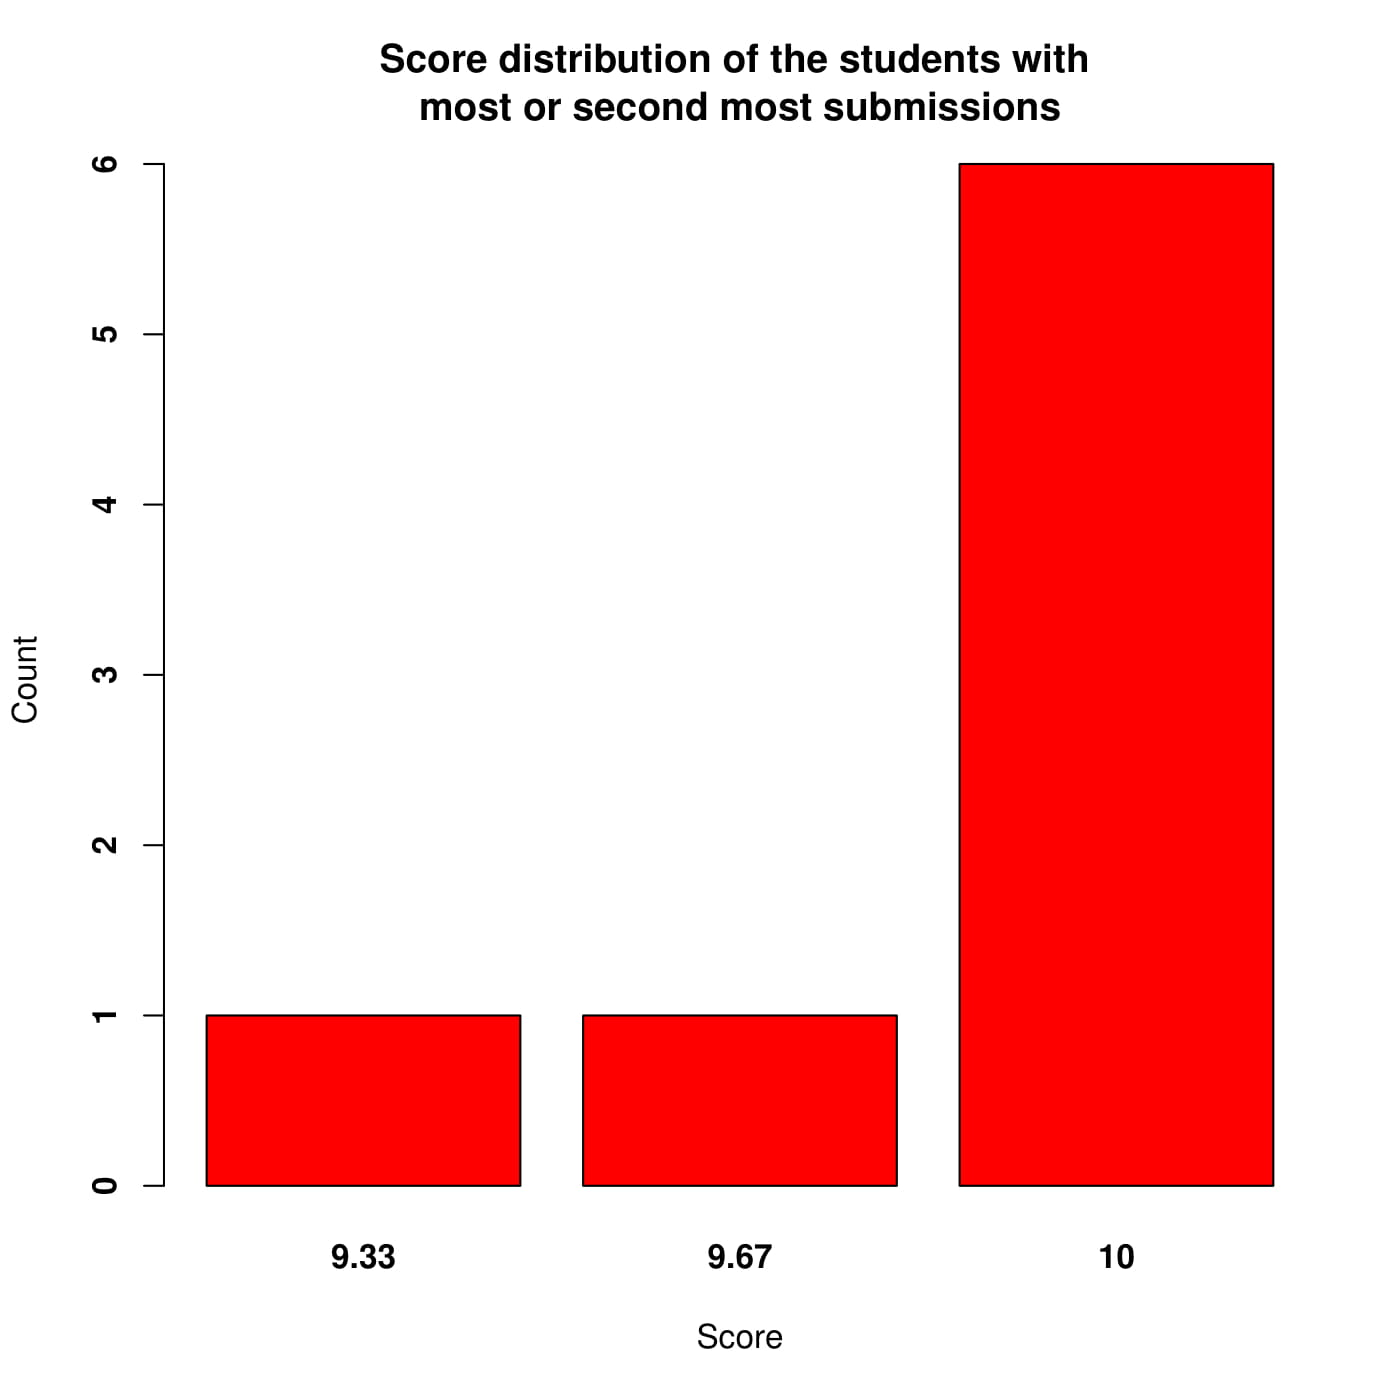
\includegraphics[width = 6.9cm]{Images/img3-4-1.png} & 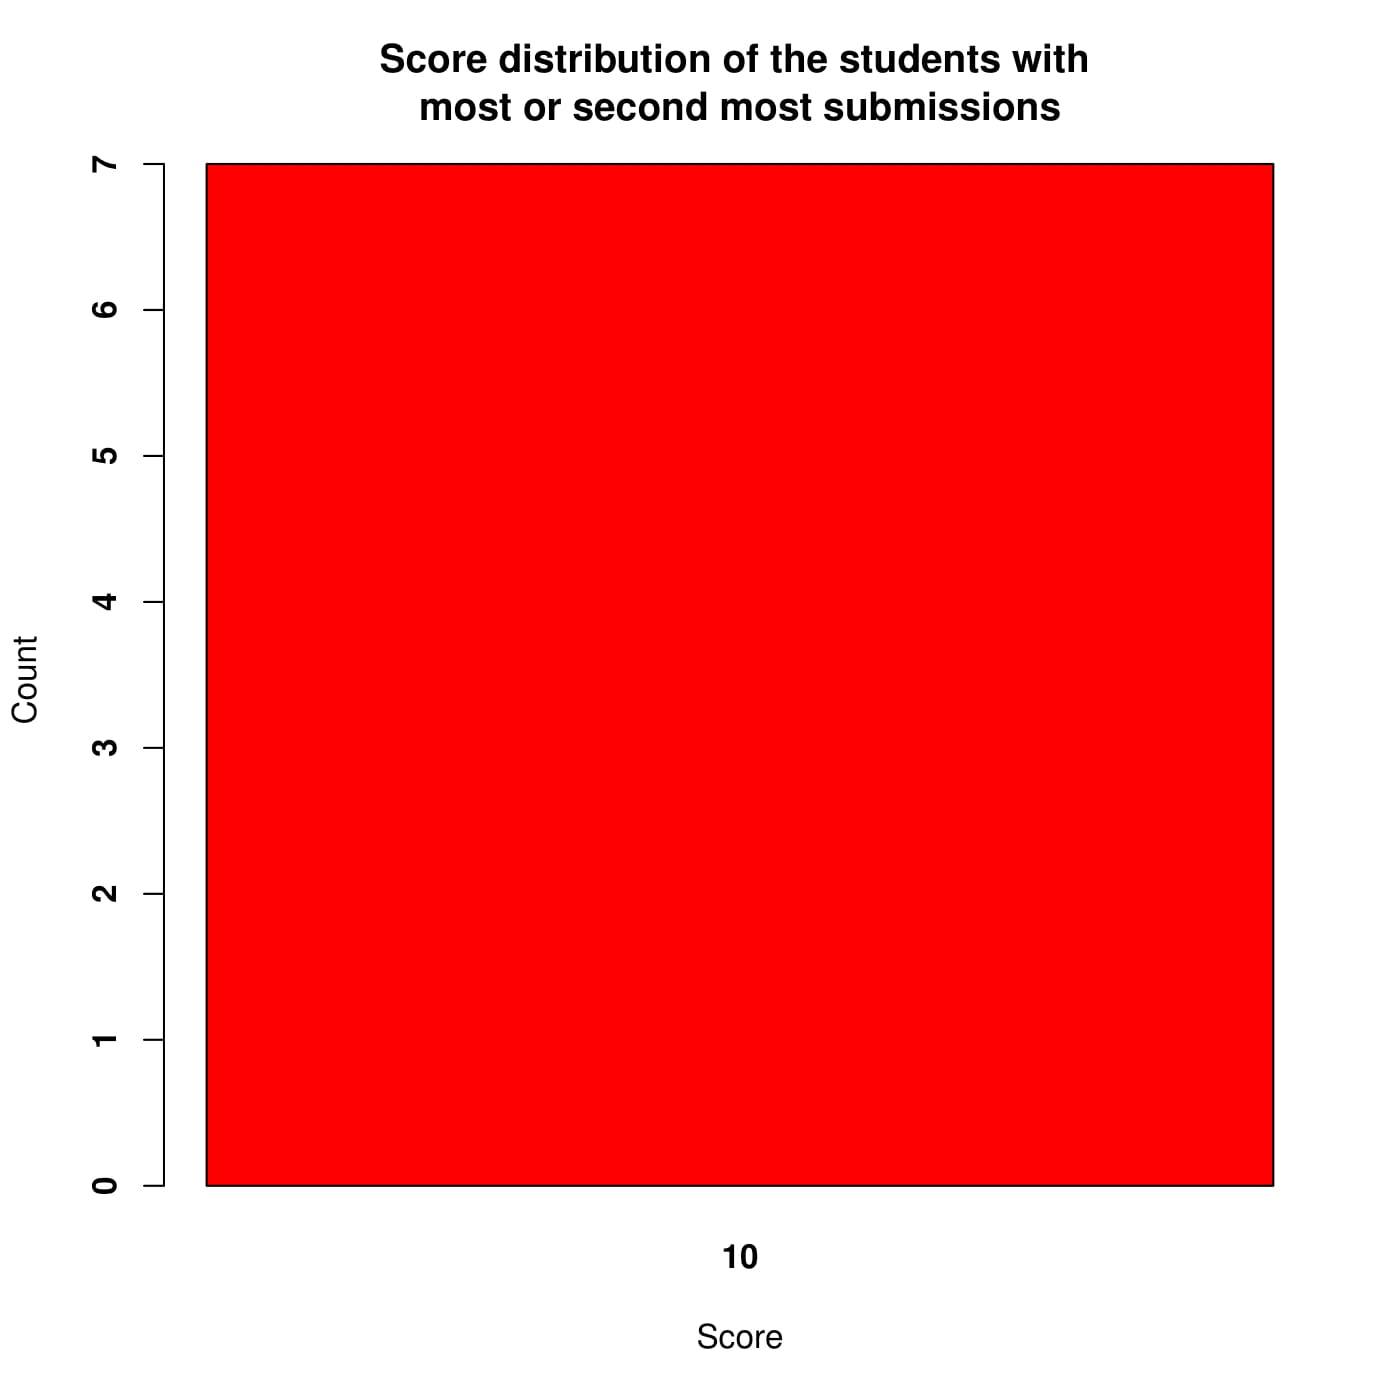
\includegraphics[width = 6.9cm]{Images/img3-4-2.png} \\
                 (1) & (2) \\
                 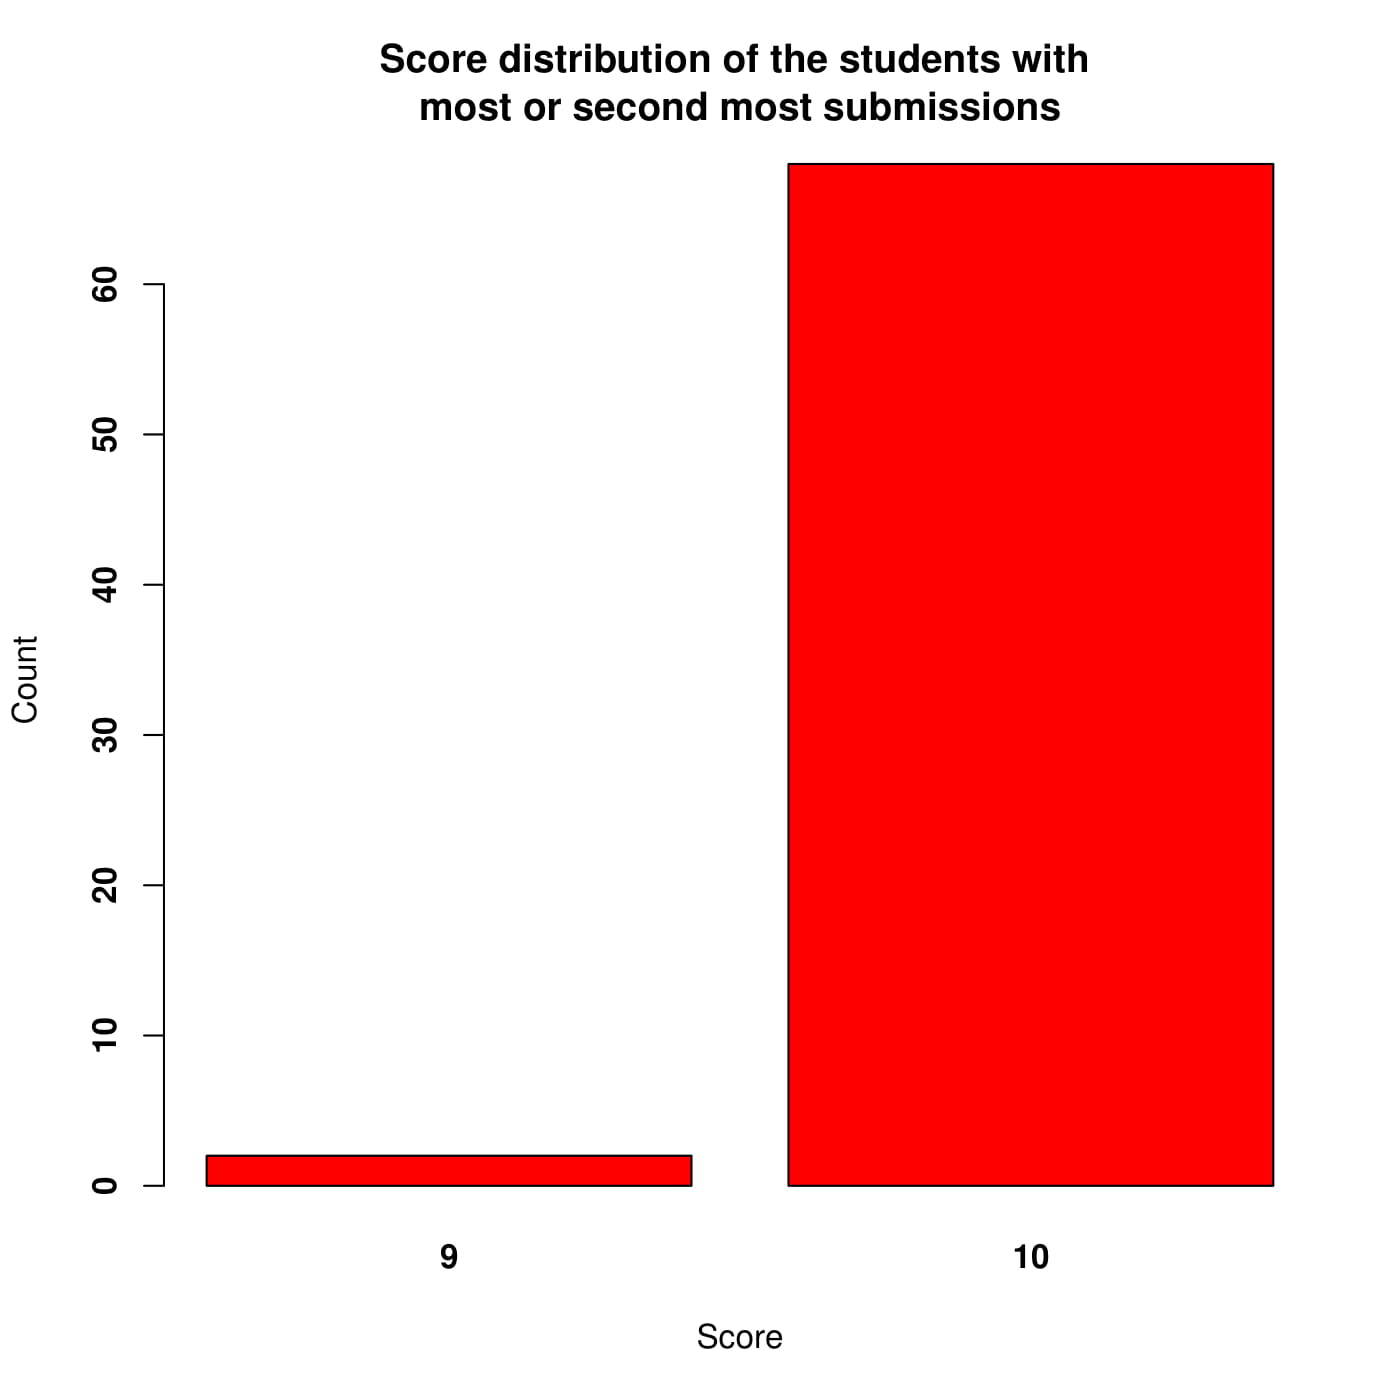
\includegraphics[width = 6.9cm]{Images/img3-4-3.png} &
                 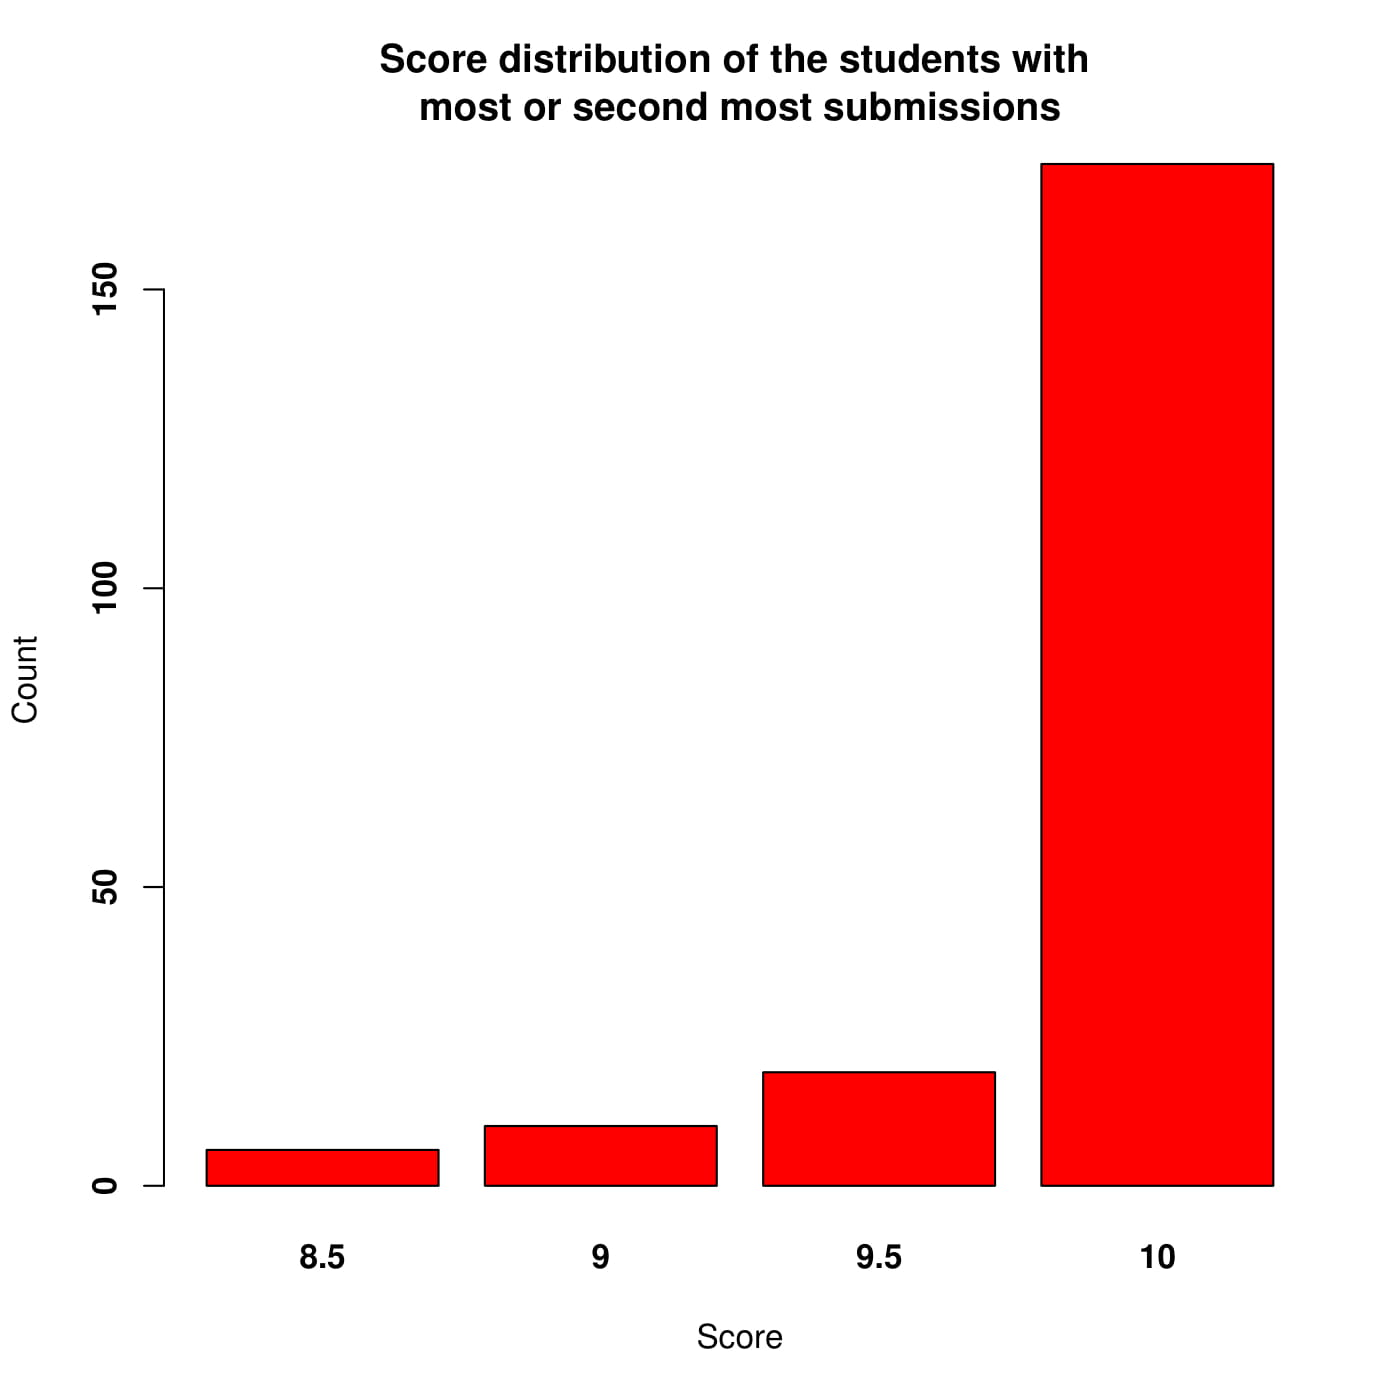
\includegraphics[width = 6.9cm]{Images/img3-4-4.png} \\
                 (3) & (4)
            \end{tabular}\\
            \textbf{Hình 3.4:} Phổ điểm của các sinh viên có số lần nộp bài nhiều nhất hoặc nhiều nhì\\
            \begin{tabular}{c c}
                 (1) & \texttt{"CO1007\_TV\_HK192-Quiz 1.4-điểm.xlsx"}\\
                 (2) & \texttt{"CO1007\_TV\_HK192-Quiz 1.5-điểm.xlsx"}\\
                 (3) & \texttt{"CO1007\_TV\_HK192-Quiz 3.3-điểm.xlsx"}\\
                 (4) & \texttt{"CO1007\_TV\_HK192-Quiz 4.2-điểm.xlsx"}
            \end{tabular}
        \end{center}
    \end{itemize}
    %Cau r
    \bf\item {Xác định danh sách các sinh viên nằm trong nhóm một phần ba đầu theo thứ tự số lần nộp bài giảm dần}\\[6pt]
    \bf Kiến thức chuẩn bị\normalfont
    \begin{itemize}
        \item Cách giải truyền thống:
        \begin{itemize}
            \item Ta sắp xếp dữ liệu theo thứ tự giảm dần của số lần nộp bài rồi lấy một phần ba đầu tiên của dữ liệu.
        \end{itemize}
    \end{itemize}
    \bf Hiện thực trên R\normalfont
    \begin{itemize}
        \item Ý tưởng thực hiện:
        \begin{itemize}
            \item Để sắp xếp dữ liệu theo thứ tự giảm dần của số lần nộp bài, ta dùng hàm $order()$. Sau đó ta lấy một phần ba đầu của danh sách bằng hàm $head()$.
            \begin{center}
                \begin{tabular}{p{13cm}}
                    \texttt{decreasing\_data <- arranged\_data[order(arranged\_data\$submission, decreasing = TRUE),]}\\
                    \texttt{top\_third <- head(decreasing\_data, length(decreasing\_data\$submission)/3)}\\
                    \texttt{top\_third\$ID}
                \end{tabular}
            \end{center}
        \end{itemize}
        \item Kết quả:
        \begin{itemize}
            \item Danh sách các sinh viên nằm trong top một phần ba theo số lần nộp bài giảm dần của mỗi file:
            \begin{center}
                \begin{tabular}{l c c c c}
                     \texttt{"CO1007\_TV\_HK192-Quiz 1.4-điểm.xlsx"} & 1910038 & 1913756 & 1910198 & 1911000 \\ & 1913186 & 1913328 & 1927007 & 1937019 \\ & 1712727 & 1910113 & 1910276 & 1910892 \\ & 1911066 & 1911185 & 1911565 & 1911704 \\ & 1912267 & 1912463 & 1912683 & 1912700\\
                     & ...\\
                     \texttt{"CO1007\_TV\_HK192-Quiz 1.5-điểm.xlsx"} & 1912817 & 1913467 & 1914768 & 1915268 \\ & 1913040 & 1914003 & 1914210 & 1712727 \\ & 1813503 & 1910123 & 1910563 & 1910666 \\ & 1911015 & 1911565 & 1911591 & 1911881 \\ & 1911900 & 1911907 & 1912046 & 1912457\\
                     & ...\\
                     \texttt{"CO1007\_TV\_HK192-Quiz 3.3-điểm.xlsx"} & 1913045 & 1915520 & 1927007 & 1511191 \\ & 1812477 & 1852443 & 1910123 & 1910409 \\ & 1910892 & 1911066 & 1911262 & 1911363 \\ & 1911441 & 1912123 & 1912288 & 1912371 \\ & 1912410 & 1912457 & 1912594 & 1912602\\
                     & ...\\
                     \texttt{"CO1007\_TV\_HK192-Quiz 4.2-điểm.xlsx"} & 1910032 & 1910060 & 1910666 & 1911000 \\ & 1911136 & 1912056 & 1912539 & 1912676 \\ & 1913045 & 1913306 & 1913355 & 1913467 \\ & 1913566 & 1913775 & 1913918 & 1914003 \\ & 1914011 & 1914093 & 1914659 & 1914713\\
                     & ...
                \end{tabular}
            \end{center}
        \end{itemize}
    \end{itemize}
    %Cau s
    \bf\item {Xác định số lượng các sinh viên nằm trong nhóm một phần ba đầu theo thứ tự số lần nộp bài giảm dần}\\[6pt]
    \bf Kiến thức chuẩn bị\normalfont
    \begin{itemize}
        \item Cách giải truyền thống:
        \begin{itemize}
            \item Đếm số lượng sinh viên trong danh sách ở câu trên ta có số lượng sinh viên nằm trong nhóm một phần ba đầu theo thứ tự số lần nộp bài giảm dần.
        \end{itemize}
    \end{itemize}
    \bf Hiện thực trên R\normalfont
    \begin{itemize}
        \item Ý tưởng thực hiện:
        \begin{itemize}
            \item Từ câu trên, ta đã có danh sách các  sinh viên nằm trong nhóm một phần ba đầu theo thứ tự số lần nộp bài giảm dần. Đếm số ID trong danh sách này bằng lệnh $length()$ ta có được số lượng sinh viên nằm trong nhóm một phần ba đầu theo thứ tự số lần nộp bài giảm dần.
            \begin{center}
                \begin{tabular}{p{13cm}}
                    \texttt{length(top\_third\$ID)}
                \end{tabular}
            \end{center}
        \end{itemize}
        \item Kết quả:
        \begin{itemize}
            \item Số lượng sinh viên nằm trong nhóm một phần ba đầu theo thứ tự số lần nộp bài giảm dần tương ứng với mỗi file
            \begin{center}
                \begin{tabular}{l l}
                     \texttt{"CO1007\_TV\_HK192-Quiz 1.4-điểm.xlsx"} & 114 sinh viên\\ 
                     \texttt{"CO1007\_TV\_HK192-Quiz 1.5-điểm.xlsx"} & 114 sinh viên\\ 
                     \texttt{"CO1007\_TV\_HK192-Quiz 3.3-điểm.xlsx"} & 93 sinh viên\\ 
                     \texttt{"CO1007\_TV\_HK192-Quiz 4.2-điểm.xlsx"} & 86 sinh viên\\ 
                \end{tabular}
            \end{center}
        \end{itemize}
    \end{itemize}
    %Cau t
    \bf\item {Xác định phổ theo điểm số của các sinh viên nằm trong nhóm một phần ba đầu theo thứ tự số lần nộp bài giảm dần}\\[6pt]
    \bf Kiến thức chuẩn bị\normalfont
    \begin{itemize}
        \item Cách giải truyền thống:
        \begin{itemize}
            \item Từ danh sách các sinh viên nằm trong nhóm một phần ba đầu theo thứ tự số lần nộp bài giảm dần ở trên, ta vẽ được phổ điểm bằng cách thống kê tần số của các điểm số.
        \end{itemize}
    \end{itemize}
    \bf Hiện thực trên R\normalfont
    \begin{itemize}
        \item Ý tưởng thực hiện:
        \begin{itemize}
            \item Ta sử dụng hàm $table()$ để thống kế tần số của các điểm số, dùng hàm $barplot()$ để vẽ phổ điểm.
            \begin{center}
                \begin{tabular}{p{13cm}}
                    \texttt{barplot(table(top\_third\$Total), xlab = "Score", ylab = "Count", col = "red", font = 2)}
                \end{tabular}
            \end{center}
        \end{itemize}
        \item Biểu đồ:\\
        \begin{center}
            \begin{tabular}{c c}
                 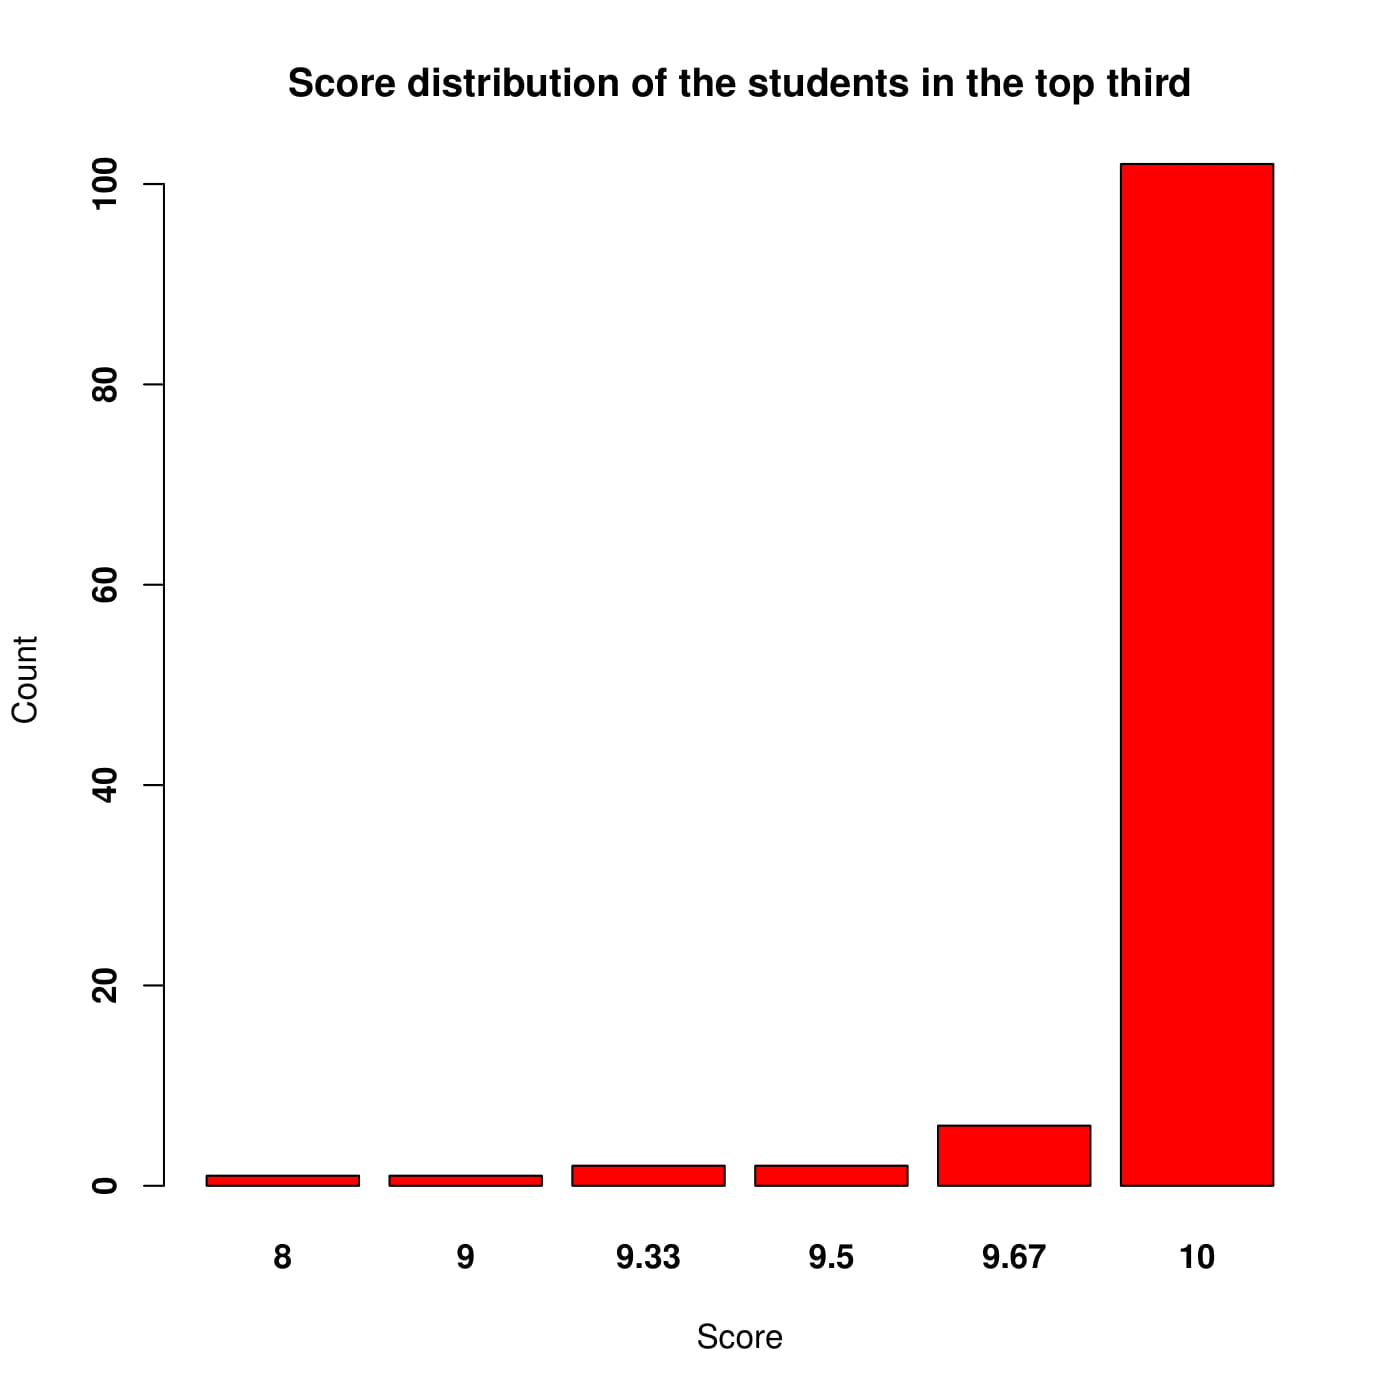
\includegraphics[width = 6.9cm]{Images/img3-5-1.png} & 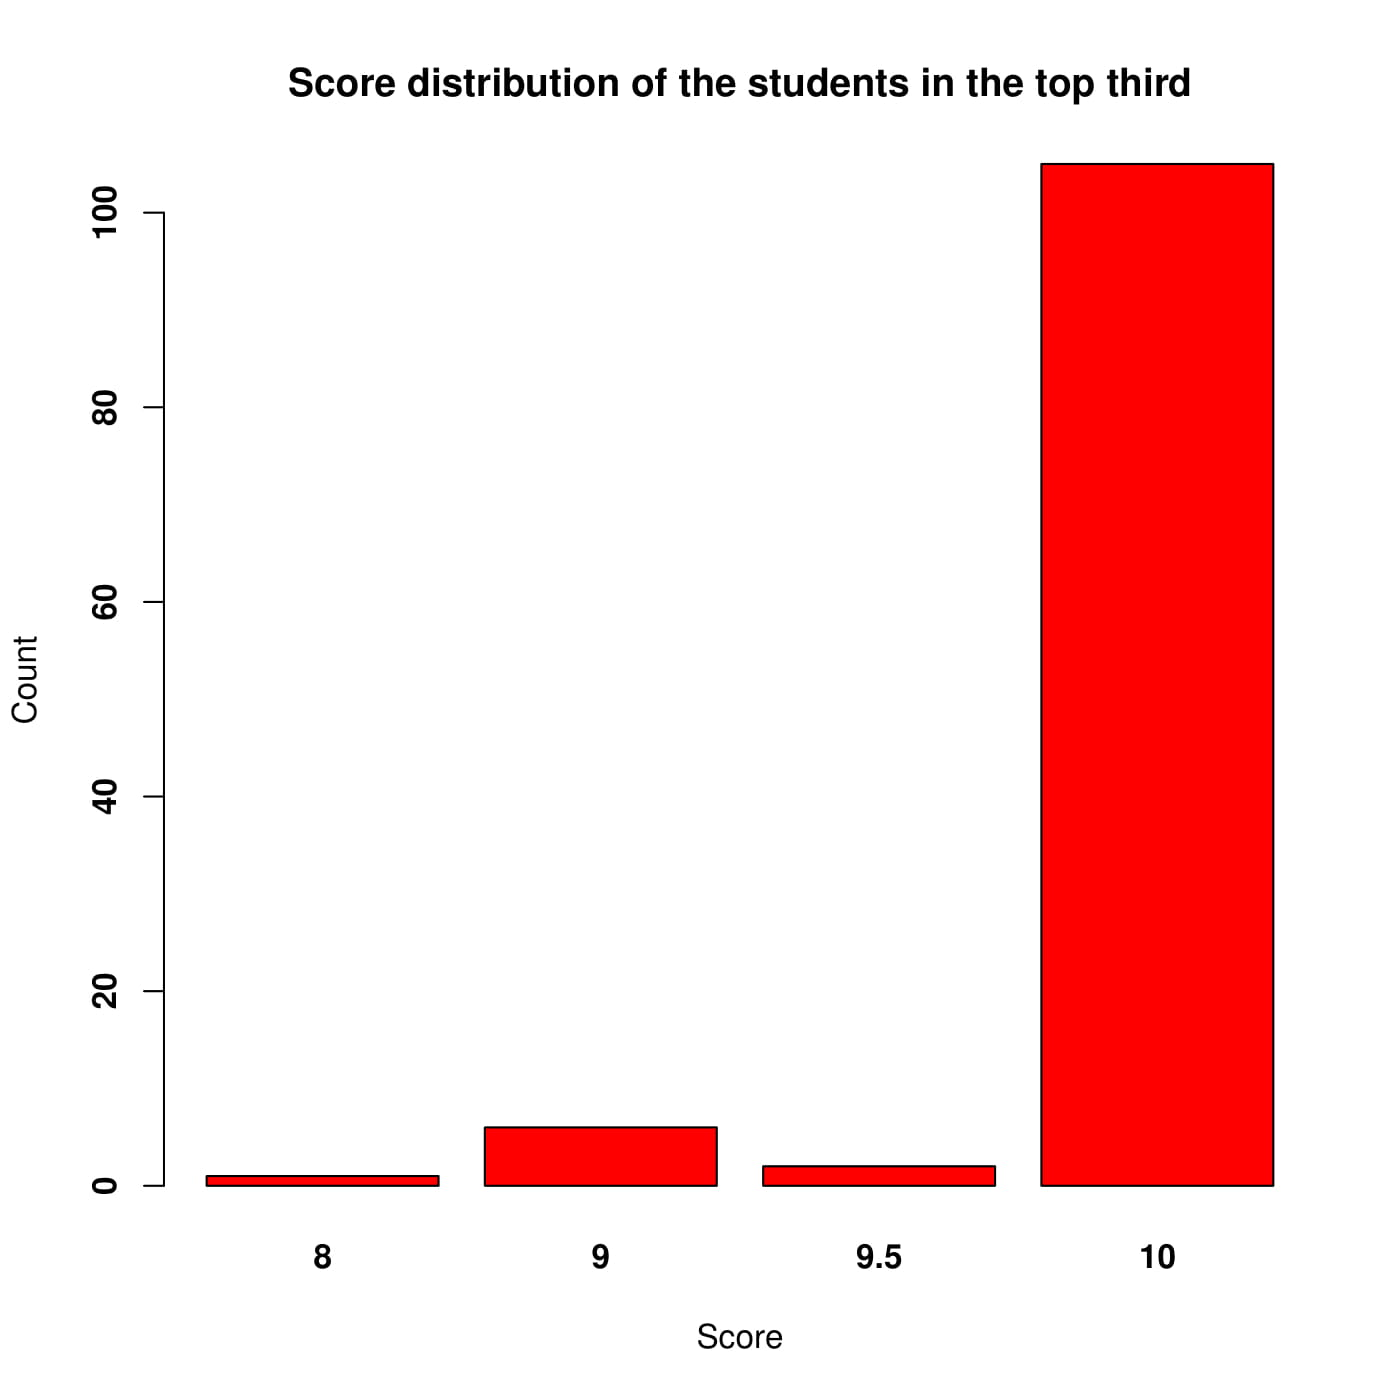
\includegraphics[width = 6.9cm]{Images/img3-5-2.png} \\
                 (1) & (2) \\
                 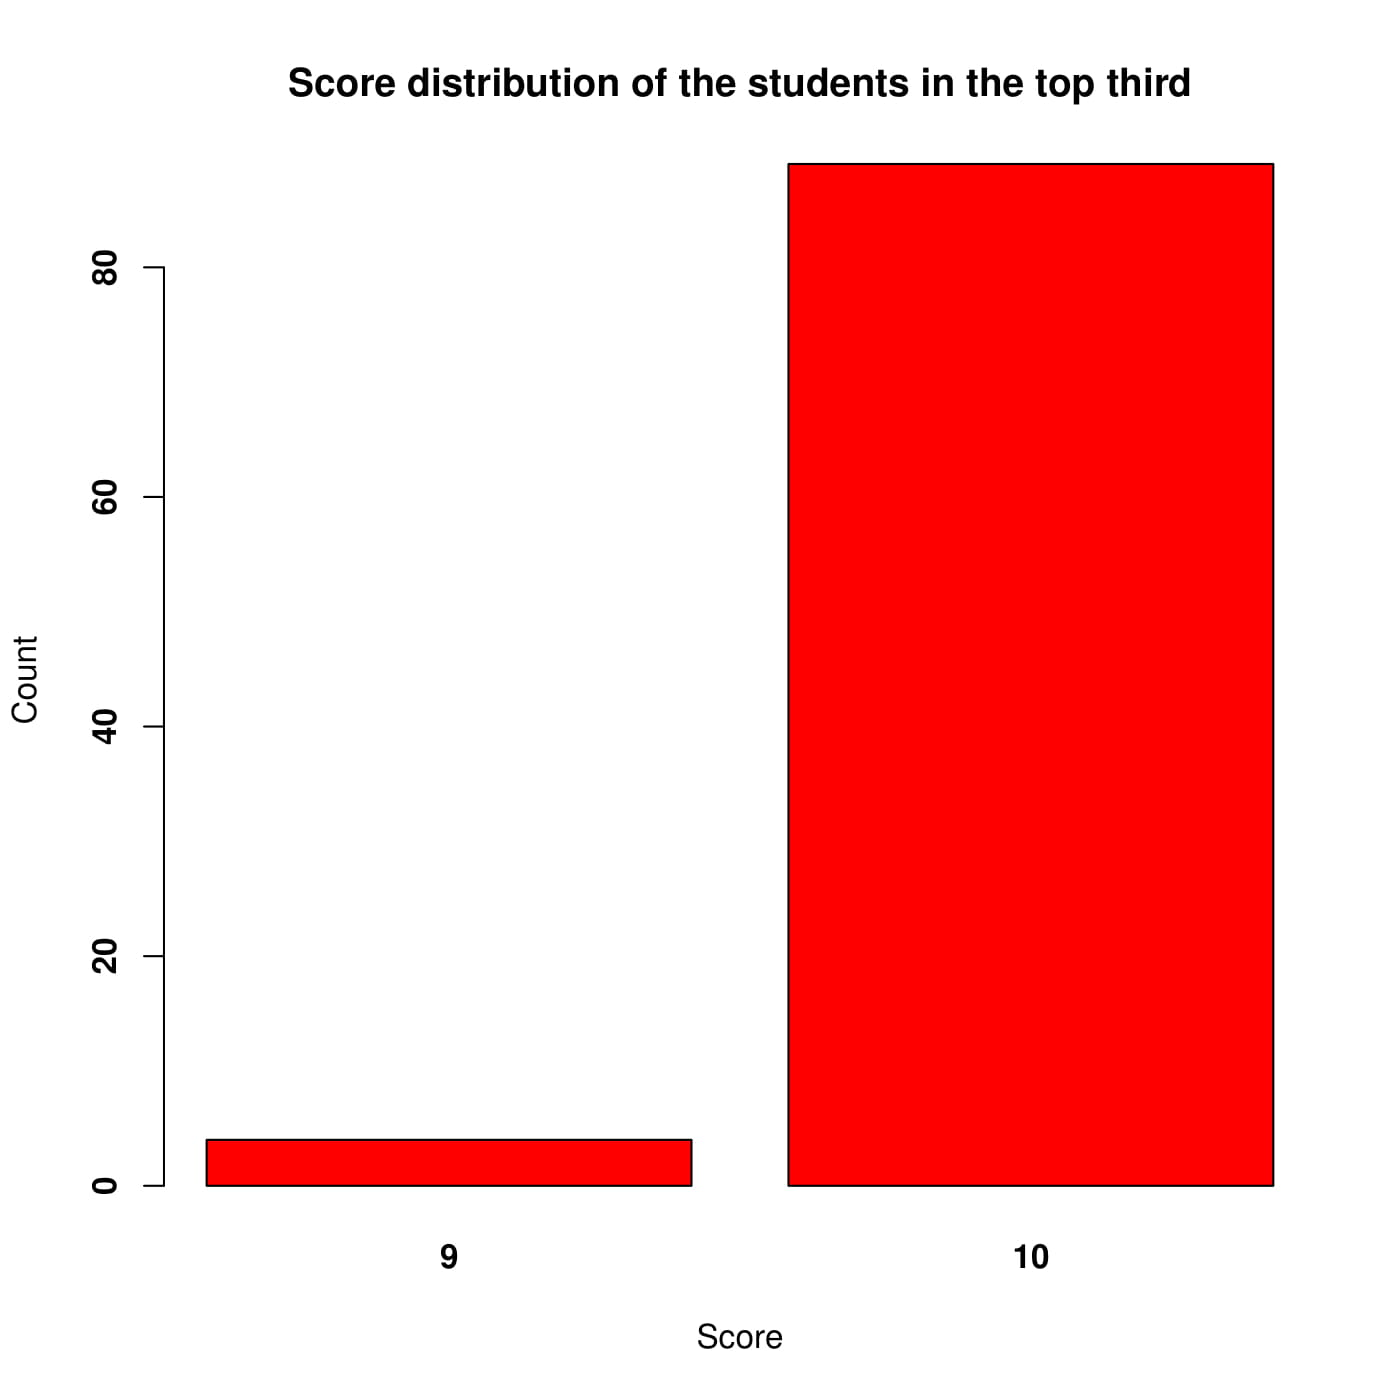
\includegraphics[width = 6.9cm]{Images/img3-5-3.png} &
                 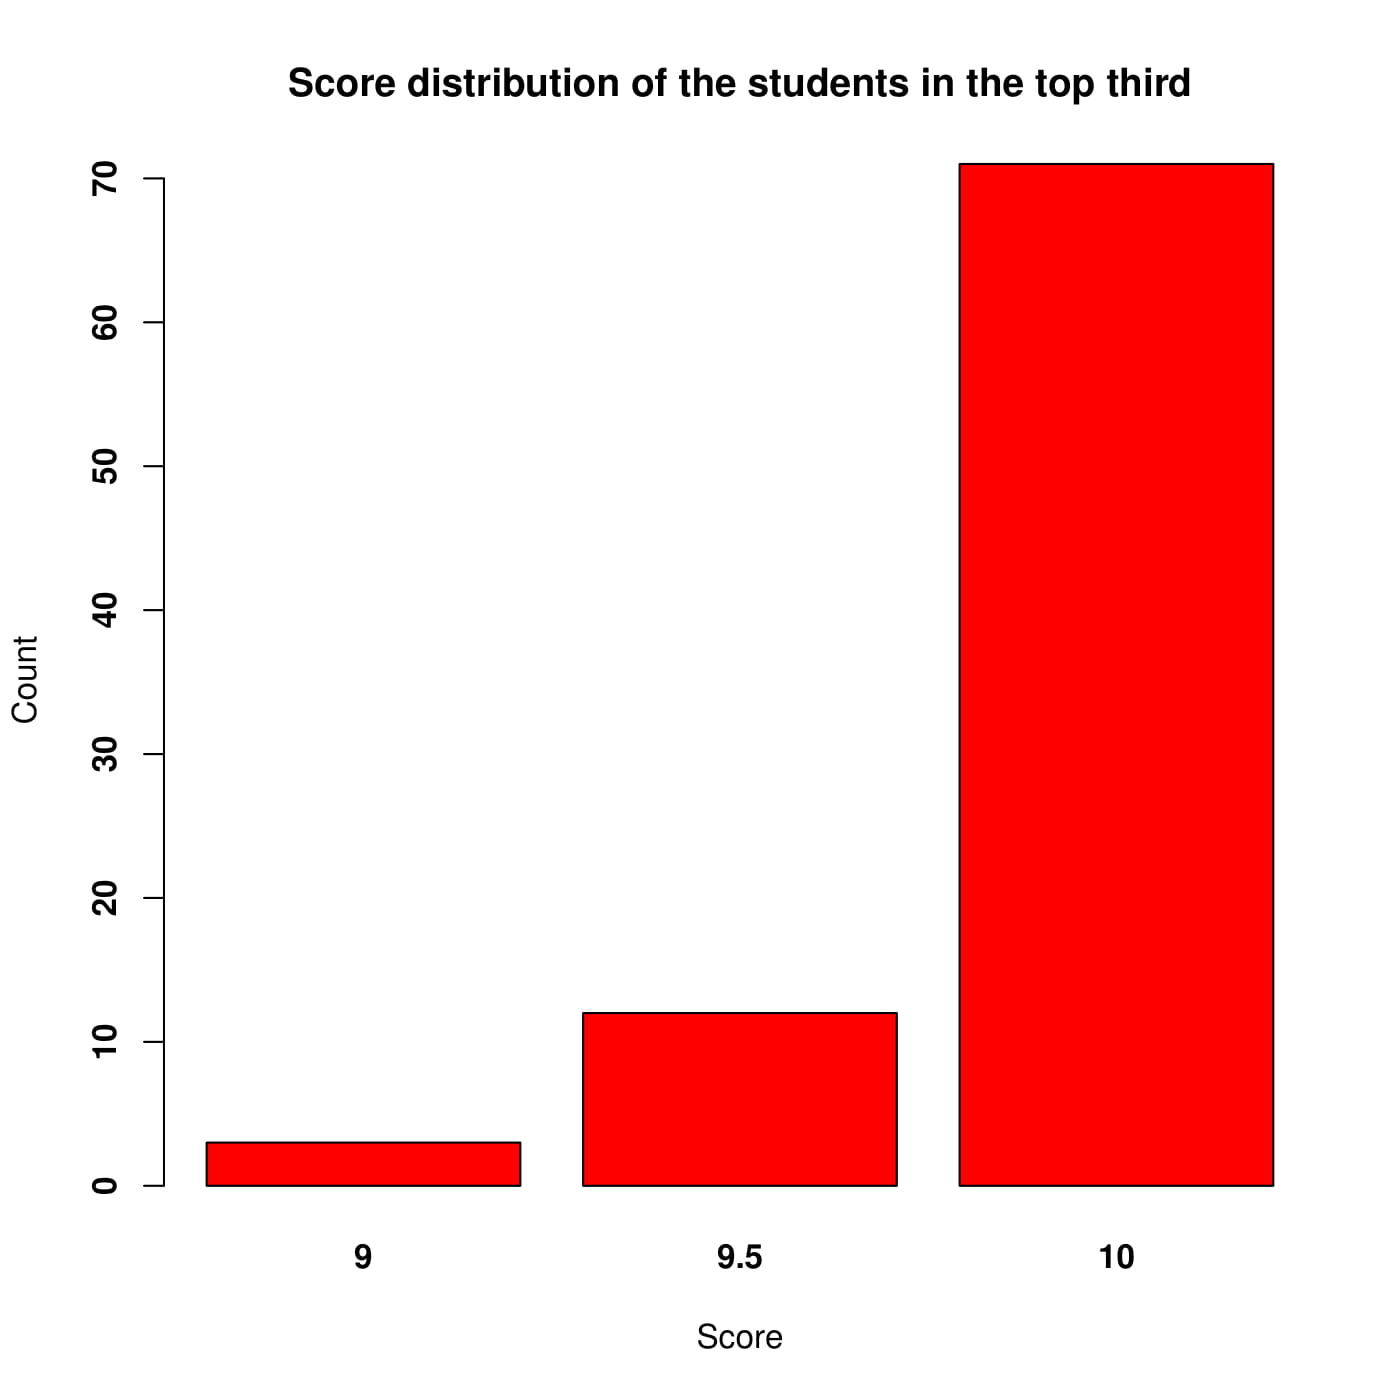
\includegraphics[width = 6.9cm]{Images/img3-5-4.png} \\
                 (3) & (4)
            \end{tabular}\\
            \textbf{Hình 3.5:} Phổ điểm của các sinh viên trong nhóm một phần ba đầu\\
            \begin{tabular}{c c}
                 (1) & \texttt{"CO1007\_TV\_HK192-Quiz 1.4-điểm.xlsx"}\\
                 (2) & \texttt{"CO1007\_TV\_HK192-Quiz 1.5-điểm.xlsx"}\\
                 (3) & \texttt{"CO1007\_TV\_HK192-Quiz 3.3-điểm.xlsx"}\\
                 (4) & \texttt{"CO1007\_TV\_HK192-Quiz 4.2-điểm.xlsx"}
            \end{tabular}
        \end{center}
    \end{itemize}
    %Cau u
    \bf\item {Xác định phổ theo điểm số của các sinh viên nằm trong $k$ nhóm đầu mà mỗi nhóm chứa các sinh viên có cùng số lần nộp bài và các nhóm được sắp xếp theo thứ tự giảm dần của có số lần nộp bài (với $k$ cho trước)}.\\[6pt]
    \bf Kiến thức chuẩn bị\normalfont
    \begin{itemize}
        \item Cách giải truyền thống:
        \begin{itemize}
            \item Từ bảng tần số của các ID, ta tìm ra được danh sách $k$ nhóm đầu ($k$ cho trước) theo thứ tự giảm dần của số lần nộp bài. Từ danh sách này, thống kê tần số của các điểm số, ta có được phổ điểm.
        \end{itemize}
    \end{itemize}
    \bf Hiện thực trên R\normalfont
    \begin{itemize}
        \item Ý tưởng thực hiện:
        \begin{itemize}
            \item $k$ là số cho trước, được nhập từ bàn phím bằng hàm $readline()$
            \begin{center}
                \begin{tabular}{p{13cm}}
                    \texttt{k <- readline(prompt = "Enter k: ")} \\
                    \texttt{k <- as.integer(k)}
                \end{tabular}
            \end{center}
            \item Trước hết ta cần tìm số lần nộp bài lớn thứ k bằng hàm $max()$ và vòng lặp for.
            \begin{center}
                \begin{tabular}{p{13cm}}
                    \texttt{if (k == 1) \{} \\
                    \hspace{0.5cm} \texttt{k\_th\_max <- max\_num} \\
                    \texttt{\}} \\
                    \texttt{else\{} \\
                    \hspace{0.5cm} \texttt{for (i in 2:k)} \\
                    \hspace{0.5cm} \texttt{\{} \\
                    \hspace{1cm} \texttt{k\_th\_max <- max(submission\_table\$freq[submission\_table\$freq < max\_temp])} \\
                    \hspace{1cm} \texttt{max\_temp <- k\_th\_max} \\
                    \hspace{0.5cm} \texttt{\}} \\
                    \texttt{\}}
                \end{tabular}
            \end{center}
            \item Số lần nộp bài lớn thứ $k$ được lưu trong biến $k\_th\_max$
            \item Sau đó ta lọc được danh sách $k$ nhóm đầu bằng hàm $subset()$. Từ danh sách này ta có được phổ điểm của các học sinh trong $k$ nhóm đầu. Ta sử dụng hàm $table()$ để thống kế tần số của các điểm số, dùng hàm $barplot()$ để vẽ phổ điểm.\\
            \begin{center}
                \begin{tabular}{p{13cm}}
                    \texttt{top\_k\_group <- subset(arranged\_data, submission >= k\_th\_max)}\\
                    \texttt{barplot(table(top\_k\_group\$Total), xlab = "Score", ylab = "Count", col = "red", font = 2)}
                \end{tabular}
            \end{center}
        \end{itemize}
        \item Biểu đồ:
        \begin{itemize}
            \item Giả sử $k=2$:
            \begin{center}
                \begin{tabular}{c c}
                     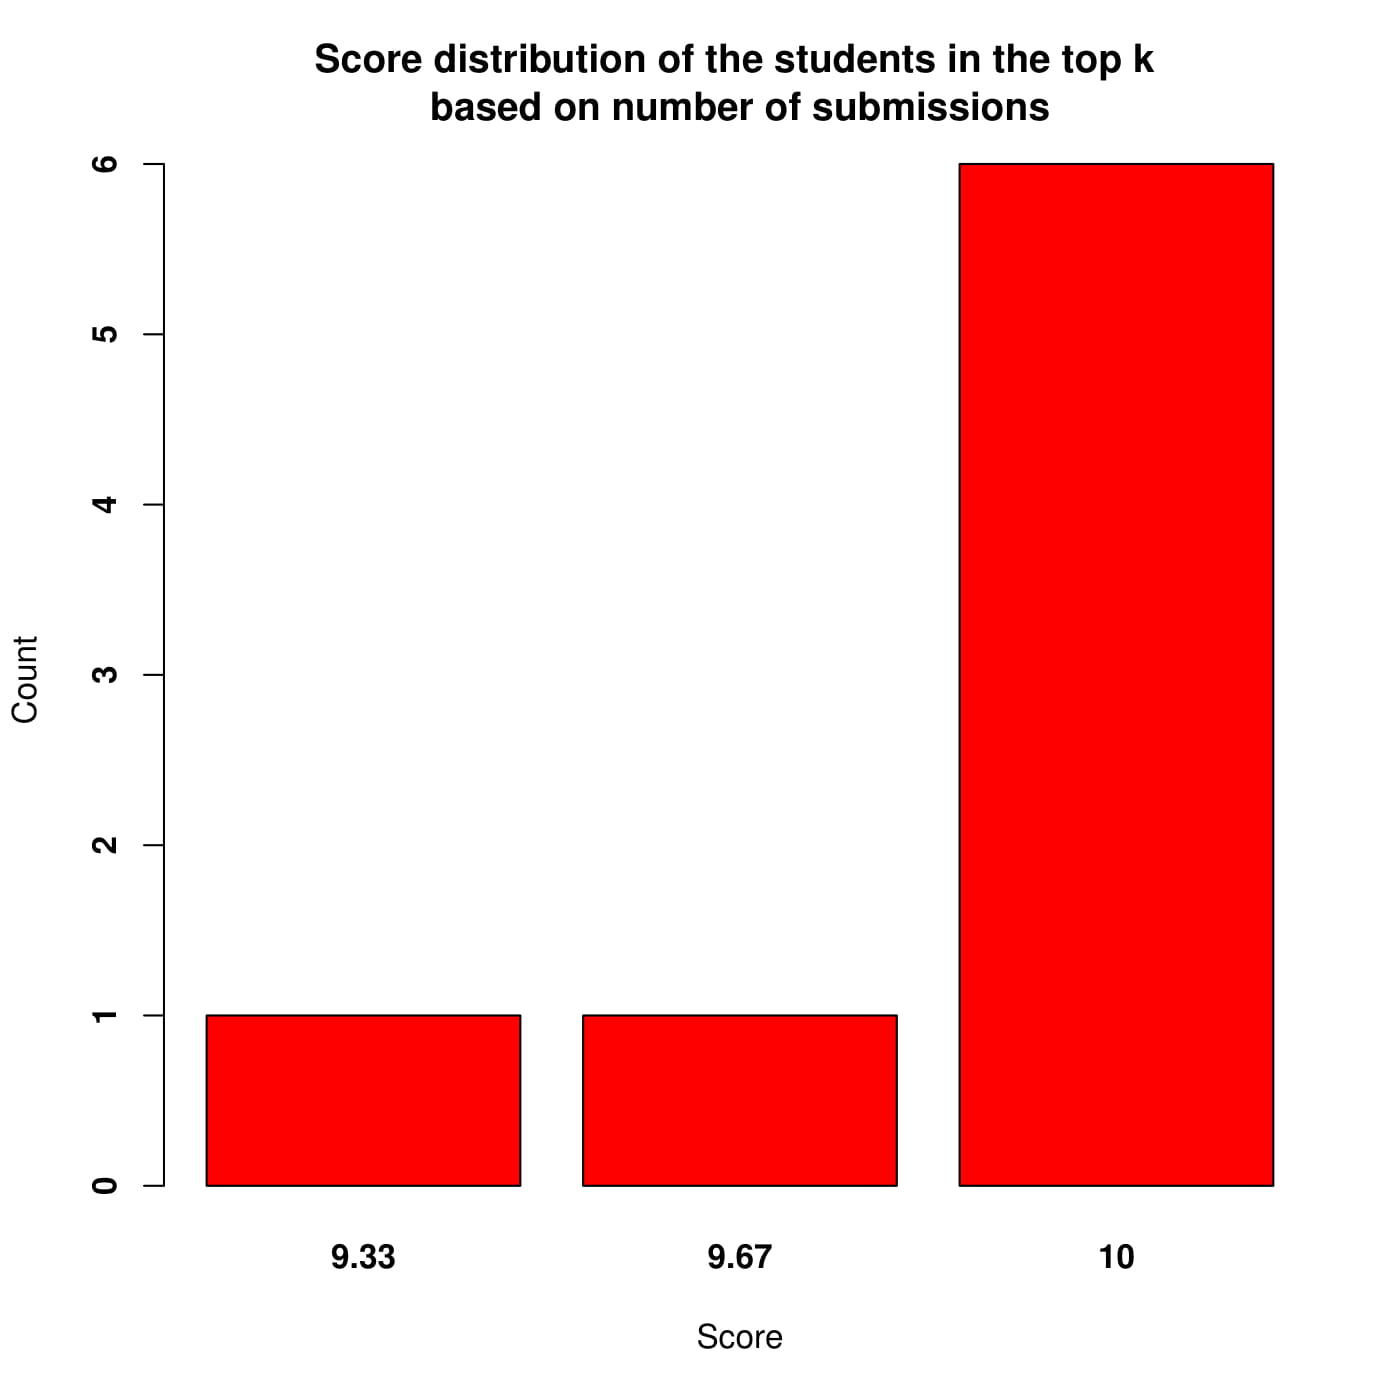
\includegraphics[width = 6.9cm]{Images/img3-6-1.png} & 
                     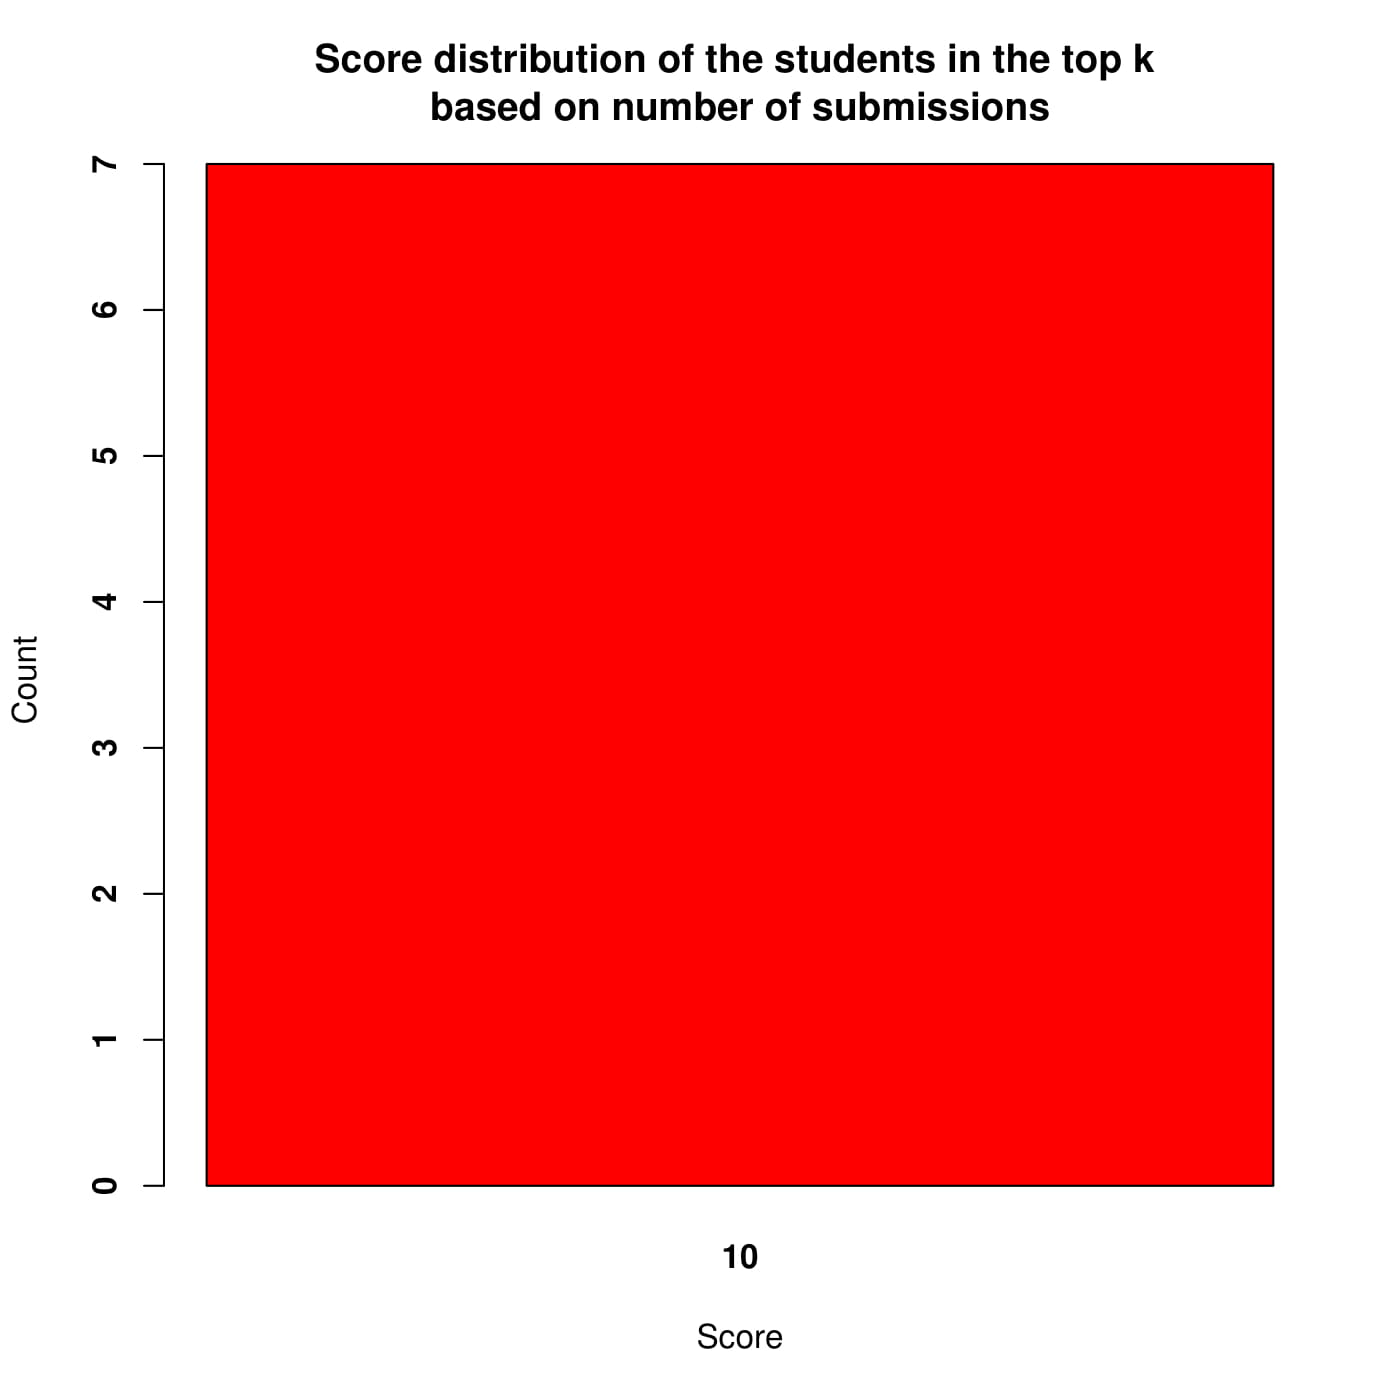
\includegraphics[width = 6.9cm]{Images/img3-6-2.png} \\
                     (1) & (2) \\
                     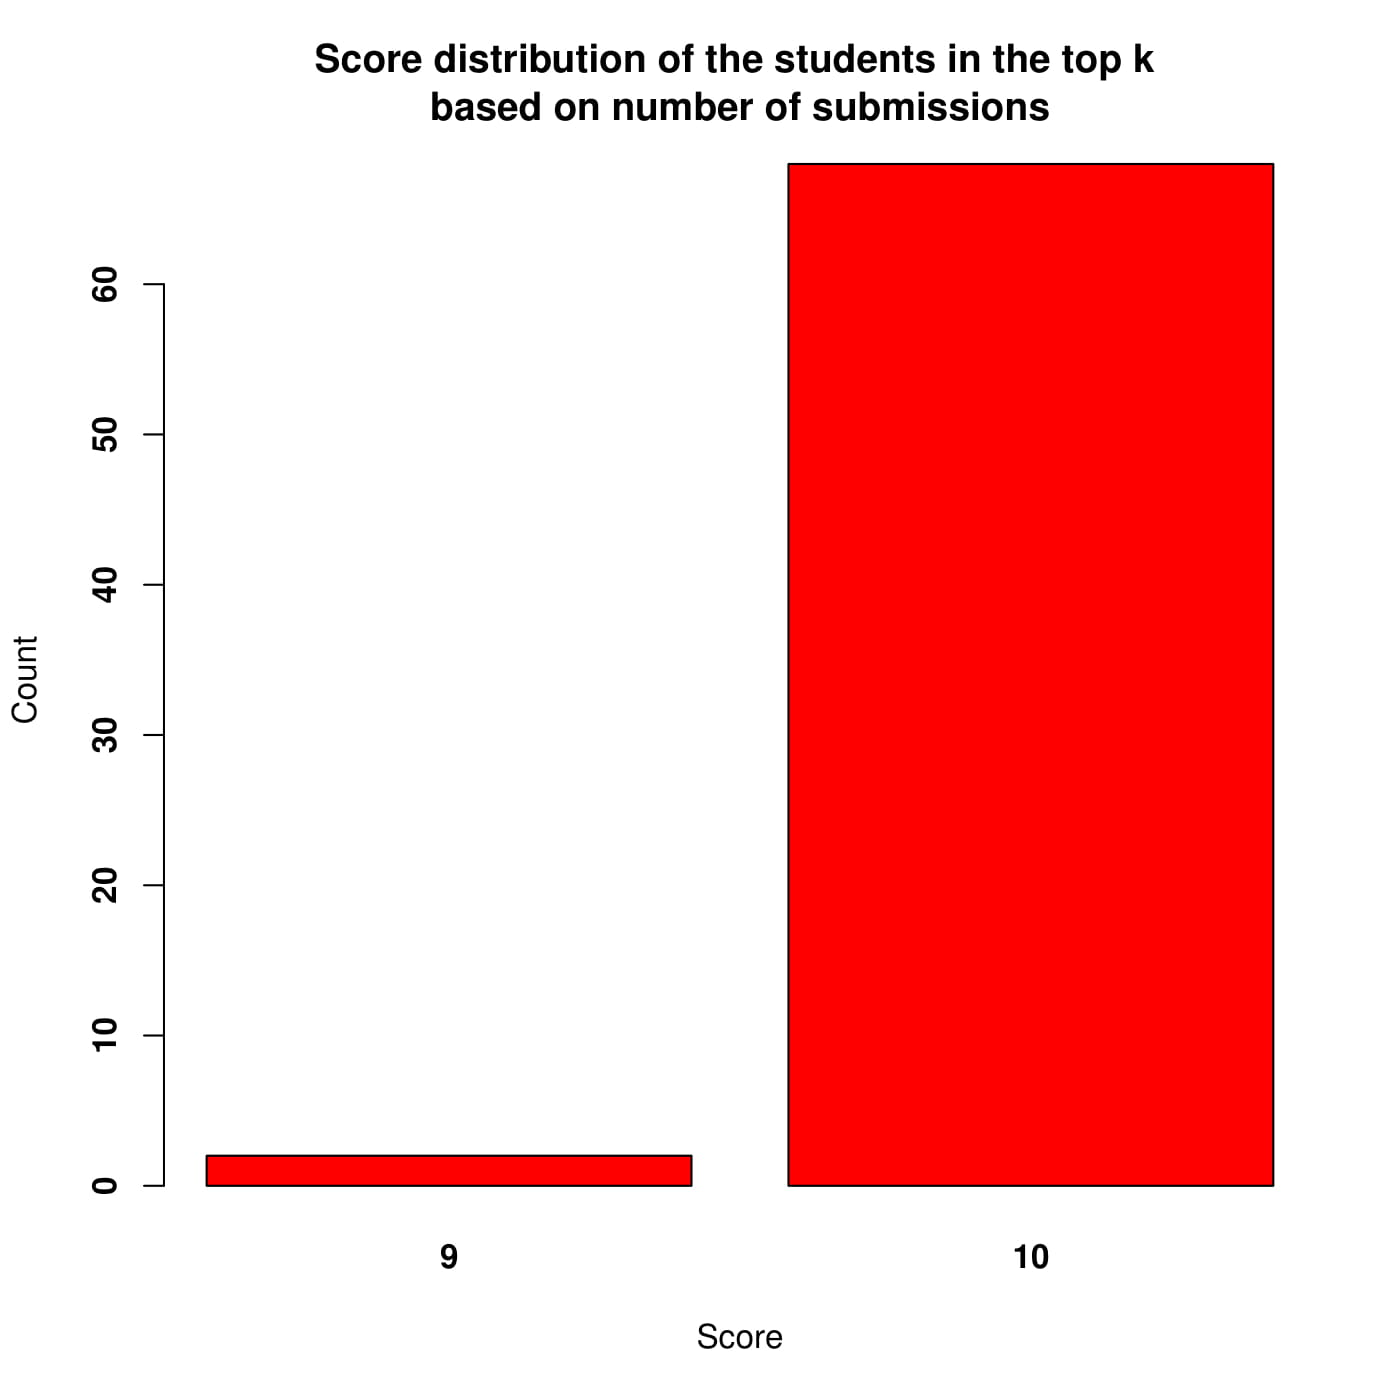
\includegraphics[width = 6.9cm]{Images/img3-6-3.png} &
                     \includegraphics[width = 6.9cm]{Images/img3-6-4.png} \\
                     (3) & (4)
                \end{tabular}\\
                \textbf{Hình 3.6:} Phổ điểm của các sinh viên trong k nhóm đầu\\
                \begin{tabular}{c c}
                     (1) & \texttt{"CO1007\_TV\_HK192-Quiz 1.4-điểm.xlsx"}\\
                     (2) & \texttt{"CO1007\_TV\_HK192-Quiz 1.5-điểm.xlsx"}\\
                     (3) & \texttt{"CO1007\_TV\_HK192-Quiz 3.3-điểm.xlsx"}\\
                     (4) & \texttt{"CO1007\_TV\_HK192-Quiz 4.2-điểm.xlsx"}
                \end{tabular}
            \end{center}
        \end{itemize}
    \end{itemize}
\end{enumerate}

%%%%%%%%%%%%%%%%%%%%%%%%%%%%%%%%%%%%%%%%%%%%%%%%%%%%%%%%%%%%%%%%%%%%%%%%%%%%%%%%%%%%%%%%%%%%%%%%%%%%%%%%
%         ->       Bai 4
%%%%%%%%%%%%%%%%%%%%%%%%%%%%%%%%%%%%%%%%%%%%%%%%%%%%%%%%%%%%%%%%%%%%%%%%%%%%%%%%%%%%%%%%%%%%%%%%%%%%%%%%
\addcontentsline{toc}{subsubsection}{Bài 4: Nhóm câu hỏi liên quan đến thời gian, tần suất nộp bài của các sinh viên}
\subsubsection*{Bài 4: Nhóm câu hỏi liên quan đến thời gian, tần suất nộp bài của các sinh viên}
\begin{enumerate}[a)]
    %Cau a
    \bf\item {Với mỗi sinh viên, xác định thời gian dài nhất tính từ lần nộp bài đầu tiên đến lần nộp cuối.}\\[6pt]
    \bf Kiến thức chuẩn bị\normalfont
    \begin{itemize}
        \item Cách giải truyền thống:
        \begin{itemize}
            \item Với mỗi sinh viên, ta lấy thời gian nộp bài cuối cùng của sinh viên đó trừ cho thời gian nộp bài đầu tiên của sinh viên đó.
        \end{itemize}
    \end{itemize}
    \bf Hiện thực trên R\normalfont
    \begin{itemize}
        \item Ý tưởng thực hiện:
        \begin{itemize}
            \item Ta tạo 2 data frame lần lượt giữ các giả trị của các lần nộp bài đầu và cuối của sinh viên, sau đó lấy hiệu 2 vector ngày tháng trong 2 data frame ta sẽ được thời gian dài nhất tính từ lúc nộp bài lần đầu cho đến lúc nộp bài lần cuối.
            \item Sử dụng hàm $max()$ để thu được giá trị thời gian dài nhất.
        \end{itemize}
        \item Kết quả:
        \begin{itemize}
            \item Thời gian dài nhất tính từ lần nộp bài đầu tiên đến lần nộp cuối tương ứng với mỗi file
            \begin{center}
                \begin{tabular}{l l}
                     \texttt{"CO1007\_TV\_HK192-Quiz 1.4-điểm.xlsx"} & 73468 phút\\ 
                     \texttt{"CO1007\_TV\_HK192-Quiz 1.5-điểm.xlsx"} & 67413 phút\\ 
                     \texttt{"CO1007\_TV\_HK192-Quiz 3.3-điểm.xlsx"} & 32769 phút\\ 
                     \texttt{"CO1007\_TV\_HK192-Quiz 4.2-điểm.xlsx"} & 30862 phút\\ 
                \end{tabular}
            \end{center}
        \end{itemize}
    \end{itemize}
    %Cau b
    \bf\item {Xác định phổ thời gian làm việc (được tính từ lần nộp bài đầu tiên đến lần nộp cuối) của các sinh viên.}\\[6pt]
    \bf Kiến thức chuẩn bị\normalfont
    \begin{itemize}
        \item Cách giải truyền thống:
        \begin{itemize}
            \item Mỗi sinh viên có một khoảng thời gian học tập online là khác nhau, qua việc các sinh viên nộp bài lần đầu và lần cuối, ta thống kê được biểu đồ biểu diễn phổ thời gian làm việc của sinh viên (theo số lượng sinh viên và hiệu thời gian giữa lần nộp đầu và cuối)
        \end{itemize}
    \end{itemize}
    \bf Hiện thực trên R\normalfont
    \begin{itemize}
        \item Ý tưởng thực hiện:
        \begin{itemize}
            \item Dùng hàm $hist()$ để vễ biểu đồ như hình bên dưới.
        \end{itemize}
        \item Biểu đồ:\\
        \begin{center}
            \begin{tabular}{c c}
                 \includegraphics[width = 6.9cm]{Images/img4-1-1.png} & 
                 \includegraphics[width = 6.9cm]{Images/img4-1-2.png} \\
                 (1) & (2) \\
                 \includegraphics[width = 6.9cm]{Images/img4-1-2.png} &
                 \includegraphics[width = 6.9cm]{Images/img4-1-3.png} \\
                 (3) & (4)
            \end{tabular}\\
            \textbf{Hình 4.1:} Phổ thời gian làm việc của các sinh viên ứng với mỗi file\\
            \begin{tabular}{c c}
                 (1) & \texttt{"CO1007\_TV\_HK192-Quiz 1.4-điểm.xlsx"}\\
                 (2) & \texttt{"CO1007\_TV\_HK192-Quiz 1.5-điểm.xlsx"}\\
                 (3) & \texttt{"CO1007\_TV\_HK192-Quiz 3.3-điểm.xlsx"}\\
                 (4) & \texttt{"CO1007\_TV\_HK192-Quiz 4.2-điểm.xlsx"}
            \end{tabular}
        \end{center}
            
    \end{itemize}
    %Cau c
    \bf\item {Tần suất nộp bài được tính bằng phân số giữa khoảng thời gian tính từ lần nộp bài đầu tiên đến lần nộp cuối và số lần nộp bài.}\\[6pt]
    \bf Kiến thức chuẩn bị\normalfont
    \begin{itemize}
        \item Cách giải truyền thống:
        \begin{itemize}
            \item Được tính bằng thương của hiệu thời gian nộp bài (như ở câu $a$) và số lần nộp bài.
        \end{itemize}
    \end{itemize}
    \bf Hiện thực trên R\normalfont
    \begin{itemize}
        \item Ý tưởng thực hiện:
        \begin{itemize}
            \item Dùng hàm $table()$ và $data.frame()$ để trích ra một data frame mới, chứa ID của sinh viên và số lần nộp bài, sau đó thực hiện phép chia như đã nói ở trên, ta được dữ liệu cần tìm.
        \end{itemize}
        \item Kết quả:
        \begin{itemize}
            \item Danh sách sinh viên kèm theo tần suất nộp bài của mỗi file:
            \begin{center}
                \begin{tabular}{l c c c c}
                     & Mã số ID & Tần suất (phút/bài nộp)\\
                     \texttt{"CO1007\_TV\_HK192-Quiz 1.4-điểm.xlsx"} & 1511191 & 1.500000e+00\\
                     & 1613010 & 1.000000e+00\\
                     & 1712727 & 2.000000e+00\\
                     & 1812257 & 0.000000e+00\\
                     & 1812477 & 2.500000e+00\\
                     & ...\\
                     \texttt{"CO1007\_TV\_HK192-Quiz 1.5-điểm.xlsx"} & 1511191 & 5.000000e-01 \\ & 1613010 & 1.500000e+00 \\ & 1712727 & 1.666667e+00 \\ & 1812257 & 0.000000e+00 \\ & 1812477 & 1.500000e+00\\
                     & ...\\
                     \texttt{"CO1007\_TV\_HK192-Quiz 3.3-điểm.xlsx"} & 1511191 & 5.000000e-01 \\ & 1613010 & 0.000000e+00 \\ & 1812257 & 0.000000e+00 \\ & 1812477 & 5.940000e+02 \\ & 1812478 & 0.000000e+00\\
                     & ...\\
                     \texttt{"CO1007\_TV\_HK192-Quiz 4.2-điểm.xlsx"} & 1613010 & 1.000000e+00 \\ & 1812257 & 0.000000e+00 \\ & 1812477 & 1.000000e+00 \\ & 1812478 & 2.000000e+00 \\ & 1813681 & 1.500000e+00\\
                     & ...
                \end{tabular}
            \end{center}
        \end{itemize}
    \end{itemize}
    %Cau d
    \bf\item {Xác định danh sách các sinh viên có tần suất nộp bài ít nhất}\\[6pt]
    \bf Kiến thức chuẩn bị\normalfont
    \begin{itemize}
        \item Cách giải truyền thống:
        \begin{itemize}
            \item Lập danh sách sinh viên kèm theo tần suất nộp bài của mỗi người. Chọn ra những sinh viên có tần suất nộp bài ít nhất.
        \end{itemize}
    \end{itemize}
    \bf Hiện thực trên R\normalfont
    \begin{itemize}
        \item Ý tưởng thực hiện:
        \begin{itemize}
            \item Trích một data frame mới chứa tần suất nộp bài của mỗi sinh viên từ data đã đọc được từ đề bài, sau đó ta chỉ trích lọc những dữ liệu có tần suất bằng tần suất nhỏ nhất.
        \end{itemize}
        \item Kết quả:
        \begin{itemize}
            \item Danh sách sinh viên có tần suất nộp bài ít nhất của mỗi file:
            \begin{center}
                \begin{tabular}{l c c c c}
                     \texttt{"CO1007\_TV\_HK192-Quiz 1.4-điểm.xlsx"} & 1812257 & 1812478 & 1813096 & 1813528 \\ & 1813681 & 1814611 & 1820028 & 1910076 \\ & 1910094 & 1910101 & 1910110 & 1910137 \\ & 1910224 & 1910238 & 1910339 & 1910346 \\ & 1910351 & 1910473 & 1910643 & 1910663\\
                     & ...\\
                     \texttt{"CO1007\_TV\_HK192-Quiz 1.5-điểm.xlsx"} &
                     1812257 & 1812478 & 1813528 & 1820028 \\ & 1910076 & 1910094 & 1910113 & 1910137 \\ & 1910198 & 1910224 & 1910265 & 1910339 \\ & 1910346 & 1910351 & 1910473 & 1910565 \\ & 1910643 & 1910650 & 1910735 & 1910984\\
                     & ...\\
                     \texttt{"CO1007\_TV\_HK192-Quiz 3.3-điểm.xlsx"} & 1613010 & 1812257 & 1812478 & 1813096 \\ & 1813681 & 1814096 & 1814518 & 1820028 \\ & 1910006 & 1910032 & 1910038 & 1910060 \\ & 1910076 & 1910094 & 1910101 & 1910110 \\ & 1910113 & 1910137 & 1910202 & 1910224\\
                     & ...\\
                     \texttt{"CO1007\_TV\_HK192-Quiz 4.2-điểm.xlsx"} & 1812257 & 1910094 & 1910110 & 1910402 \\ & 1910473 & 1910663 & 1910984 & 1911015 \\ & 1911056 & 1911185 & 1911283 & 1911285 \\ & 1911565 & 1911569 & 1911594 & 1911704 \\ & 1911837 & 1911841 & 1911931 & 1912041\\
                     & ...
                \end{tabular}
            \end{center}
        \end{itemize}
    \end{itemize}
    %cau e
    \bf\item {Xác định phổ điểm của các sinh viên có tần suất nộp bài ít nhất}\\[6pt]
    \bf Kiến thức chuẩn bị\normalfont
    \begin{itemize}
        \item Cách giải truyền thống:
        \begin{itemize}
            \item Tương tự câu $d$, ta liệt kê các sinh viên có tần suất nộp bài ít nhất và vẽ phổ điểm của các sinh viên ấy.
        \end{itemize}
    \end{itemize}
    \bf Hiện thực trên R\normalfont
    \begin{itemize}
        \item Ý tưởng thực hiện:
        \begin{itemize}
            \item Từ data rút ra một data frame (gọi là A) gồm ID của các sinh viên và điểm số cao nhất của mỗi sinh viên. Đồng thời ta đã có một data frame từ câu $c$ và $d$ (gọi là B). Rút từ B ra các sinh viên có tần suất nộp bài thấp nhất. Sau đó dùng hàm $subset()$ trích lọc ra từ A, ta có được một data frame mới chứa dữ liệu của sinh viên có tần suất nộp bài ít nhất, từ đó in ra phổ điểm bằng hàm $hist()$.
            \item Trong bài này ta sử dụng các hàm: $subset()$, $hist()$, $unique()$, $match()$.
        \end{itemize}
        \item Biểu đồ:\\
        \begin{center}
        \begin{tabular}{c c}
             \includegraphics[width = 6.9cm]{Images/img4-2-1.png} & 
             \includegraphics[width = 6.9cm]{Images/img4-2-2.png} \\
             (1) & (2) \\
             \includegraphics[width = 6.9cm]{Images/img4-2-3.png} &
             \includegraphics[width = 6.9cm]{Images/img4-2-4.png} \\
             (3) & (4)
        \end{tabular}\\
        \textbf{Hình 4.2:} Phổ điểm của các sinh viên với tần suất nộp bài thấp nhất\\
        \begin{tabular}{c c}
             (1) & \texttt{"CO1007\_TV\_HK192-Quiz 1.4-điểm.xlsx"}\\
             (2) & \texttt{"CO1007\_TV\_HK192-Quiz 1.5-điểm.xlsx"}\\
             (3) & \texttt{"CO1007\_TV\_HK192-Quiz 3.3-điểm.xlsx"}\\
             (4) & \texttt{"CO1007\_TV\_HK192-Quiz 4.2-điểm.xlsx"}
        \end{tabular}
    \end{center}
            
    \end{itemize}
    %Cau f
    \bf\item {Xác định số lượng sinh viên có tần suất nộp bài nhiều nhất}\\[6pt]
    \bf Kiến thức chuẩn bị\normalfont
    \begin{itemize}
        \item Cách giải truyền thống:
        \begin{itemize}
            \item Lập danh sách sinh viên kèm theo tần suất nộp bài của mỗi người. Chọn ra những sinh viên có tần suất nộp bài nhiều nhất. Đếm số lượng sinh viên.
        \end{itemize}
    \end{itemize}
    \bf Hiện thực trên R\normalfont
    \begin{itemize}
        \item Ý tưởng thực hiện:
        \begin{itemize}
            \item Tương tự với câu $d$, đối với bài này ta chỉ trích lọc những dữ liệu có tần suất bằng tần suất lớn nhất. Đếm số lượng sinh viên có trong tập này cho ta kết quả về số lượng sinh viên có tần suất nộp bài nhiều nhất.
        \end{itemize}
        \item Kết quả:
        \begin{itemize}
            \item Số lượng sinh viên có tần suất nộp bài lớn nhất đối với mỗi file:
            \begin{center}
                \begin{tabular}{l l}
                     \texttt{"CO1007\_TV\_HK192-Quiz 1.4-điểm.xlsx"} & 1 sinh viên\\ 
                     \texttt{"CO1007\_TV\_HK192-Quiz 1.5-điểm.xlsx"} & 1 sinh viên\\ 
                     \texttt{"CO1007\_TV\_HK192-Quiz 3.3-điểm.xlsx"} & 1 sinh viên\\ 
                     \texttt{"CO1007\_TV\_HK192-Quiz 4.2-điểm.xlsx"} & 1 sinh viên\\ 
                \end{tabular}
            \end{center}
        \end{itemize}
    \end{itemize}
    %Cau g
    \bf\item {Xác định các sinh viên có tần suất nộp bài nhiều nhất.}\\[6pt]
    \bf Kiến thức chuẩn bị\normalfont
    \begin{itemize}
        \item Cách giải truyền thống:
        \begin{itemize}
            \item Làm tương tự câu $f$. Ta lập danh sách những sinh viên có tần suất nộp bài cao nhất từ dữ liệu đã trích lọc.
        \end{itemize}
    \end{itemize}
    \bf Hiện thực trên R\normalfont
    \begin{itemize}
        \item Ý tưởng thực hiện:
        \begin{itemize}
            \item Sau khi đã trích lọc dữ liệu từ câu $f$, ta in ra bảng danh sách những sinh viên thỏa mãn tần suất nộp bài bằng tần suất nộp bài cao nhất.
            \item Ta sử dụng các hàm $max()$, $subset()$ trong bài này
        \end{itemize}
        \item Kết quả:
        \begin{itemize}
            \item Các sinh viên có tần suất nộp bài nhiều nhất của mỗi file:
            \begin{center}
                \begin{tabular}{l c c c c}
                     \texttt{"CO1007\_TV\_HK192-Quiz 1.4-điểm.xlsx"} & 1914477\\
                     \texttt{"CO1007\_TV\_HK192-Quiz 1.5-điểm.xlsx"} & 1911185\\
                     \texttt{"CO1007\_TV\_HK192-Quiz 3.3-điểm.xlsx"} & 1915442\\
                     \texttt{"CO1007\_TV\_HK192-Quiz 4.2-điểm.xlsx"} & 1936024
                \end{tabular}
            \end{center}
        \end{itemize}
    \end{itemize}
    %Cau h
    \bf\item {Xác định phổ điểm của các sinh viên có tần suất nộp bài nhiều nhất.}\\[6pt]
    \bf Kiến thức chuẩn bị\normalfont
    \begin{itemize}
        \item Cách giải truyền thống:
        \begin{itemize}
            \item Tương tự câu f, ta liệt kê các sinh viên có tần suất nộp bài nhiều nhất và vẽ phổ điểm của các sinh viên ấy.
        \end{itemize}
    \end{itemize}
    \bf Hiện thực trên R\normalfont
    \begin{itemize}
        \item Ý tưởng thực hiện:
        \begin{itemize}
            \item Các bước hiện thực tương tự câu f, ta lọc dữ liệu gồm những sinh viên có tần suất nộp bài cao nhất, sau đó vẽ phổ điểm dựa trên dữ liệu đã trích lọc bằng hàm $hist()$.
            \item Trong bài này ta sử dụng các hàm: $subset()$, $hist()$, $unique()$, $match()$.
        \end{itemize}
        \item Biểu đồ:\\
        \begin{center}
            \begin{tabular}{c c}
                 \includegraphics[width = 6.9cm]{Images/img4-3-1.png} & \includegraphics[width = 6.9cm]{Images/img4-3-2.png} \\
                 (1) & (2) \\
                 \includegraphics[width = 6.9cm]{Images/img4-3-3.png} &
                 \includegraphics[width = 6.9cm]{Images/img4-3-4.png} \\
                 (3) & (4)
            \end{tabular}\\
            \textbf{Hình 4.3:} Phổ điểm của các sinh viên với tần suất nộp bài cao nhất\\
            \begin{tabular}{c c}
                 (1) & \texttt{"CO1007\_TV\_HK192-Quiz 1.4-điểm.xlsx"}\\
                 (2) & \texttt{"CO1007\_TV\_HK192-Quiz 1.5-điểm.xlsx"}\\
                 (3) & \texttt{"CO1007\_TV\_HK192-Quiz 3.3-điểm.xlsx"}\\
                 (4) & \texttt{"CO1007\_TV\_HK192-Quiz 4.2-điểm.xlsx"}
            \end{tabular}
        \end{center}
    \end{itemize}
    %Cau i
    \bf\item {Xác định các sinh viên nằm trong nhóm có tần suất nộp bài nhiều nhì.}\\[6pt]
    \bf Kiến thức chuẩn bị\normalfont
    \begin{itemize}
        \item Cách giải truyền thống:
        \begin{itemize}
            \item Sắp xếp lại các tần suất nộp bài của sinh viên từ cao xuống thấp, lọc ra những bạn sinh viên có tần suất nộp bài nhiều nhì.
        \end{itemize}
    \end{itemize}
    \bf Hiện thực trên R\normalfont
    \begin{itemize}
        \item Ý tưởng thực hiện:
        \begin{itemize}
            \item Đầu tiên, ta dùng hàm $subset()$ trích lọc data frame không có những sinh viên có tần suất nộp bài nhiều nhất. Sau đó lại dùng hàm $subset()$ trích lọc data frame vừa thu được nhưng lần này là trích lọc những sinh viên có tần suất nhiều nhất. Suy ra, ta được danh sách những sinh viên có tần suất nộp nhiều nhì.
        \end{itemize}
        \item Kết quả:
        \begin{itemize}
            \item Các sinh viên có tần suất nộp bài nhiều nhì của mỗi file:
            \begin{center}
                \begin{tabular}{l c c c c}
                     \texttt{"CO1007\_TV\_HK192-Quiz 1.4-điểm.xlsx"} & 1911185\\
                     \texttt{"CO1007\_TV\_HK192-Quiz 1.5-điểm.xlsx"} & 1914093\\
                     \texttt{"CO1007\_TV\_HK192-Quiz 3.3-điểm.xlsx"} & 1915520\\
                     \texttt{"CO1007\_TV\_HK192-Quiz 4.2-điểm.xlsx"} & 1915775
                \end{tabular}
            \end{center}
        \end{itemize}
    \end{itemize}
    %Cau j
    \bf\item {Xác định các sinh viên nằm trong nhóm có tần suất  nộp bài nhiều nhất hoặc nhiều nhì.}\\[6pt]
    \bf Kiến thức chuẩn bị\normalfont
    \begin{itemize}
        \item Cách giải truyền thống:
        \begin{itemize}
            \item Sắp xếp lại các tần suất nộp bài của sinh viên từ cao xuống thấp, lọc ra những bạn sinh viên có tần suất nộp bài nhiều nhất hoặc nhiều nhì.
        \end{itemize}
    \end{itemize}
    \bf Hiện thực trên R\normalfont
    \begin{itemize}
        \item Ý tưởng thực hiện:
        \begin{itemize}
            \item Để lọc ra danh sách các sinh viên có tần suất nộp bài nhiều nhất hoặc nhiều nhì, ta dùng lại dữ liệu vừa mới tạo từ câu i, sử dụng hàm $subset()$ với dữ liệu trên với điều kiện giá trị của tần suất nộp bài lớn hơn hoặc bằng câu i. Như vậy, ta được danh sách các sinh viên có tần suất nộp bài nhiều nhất và nhiều nhì.
        \end{itemize}
        \item Kết quả:
        \begin{itemize}
            \item Các sinh viên có tần suất nộp bài nhiều nhất hoặc nhì của mỗi file:
            \begin{center}
                \begin{tabular}{l c c c c}
                     \texttt{"CO1007\_TV\_HK192-Quiz 1.4-điểm.xlsx"} & 1911185 & 1914477\\
                     \texttt{"CO1007\_TV\_HK192-Quiz 1.5-điểm.xlsx"} & 1914093 & 1911185\\
                     \texttt{"CO1007\_TV\_HK192-Quiz 3.3-điểm.xlsx"} & 1915520 & 1915442\\
                     \texttt{"CO1007\_TV\_HK192-Quiz 4.2-điểm.xlsx"} & 1915775 & 1936024
                \end{tabular}
            \end{center}
        \end{itemize}
    \end{itemize}
    %Cau k
    \bf\item Hãy tính thời gian trung bình (tính bằng giây) giữa hai lần nộp bài liền nhau của cùng một sinh viên trong mẫu đã chọn.\\[6pt]
    \bf Kiến thức chuẩn bị\normalfont
    \begin{itemize}
        \item Cách giải truyền thống:
        \begin{itemize}
            \item Để tính thời gian giữa các lần nộp bài trung bình, ta lấy trung bình của $n-1$ giá trị thời gian giữa hai lần nộp bài liên tiếp, với $n$ là số lần nộp bài của sinh viên đó.
            \item Giá trị này cũng có thể xác định bằng công thức:
            \begin{center}
                $\overline{\Delta t} = \frac{t_{last} - t_{first}}{n - 1}$\\
                \begin{tabular}{p{13cm}}
                     \begin{tabular}{l l}
                          trong đó: & $t_{last}$ là thời gian nộp bài cuối cùng\\
                          & $t_{first}$ là thời gian nộp bài đầu tiên\\
                          & $n$ là số lần nộp bài
                     \end{tabular}
                \end{tabular}
            \end{center}
        \end{itemize}
    \end{itemize}
    \bf Hiện thực trên R\normalfont
    \begin{itemize}
        \item Ý tưởng thực hiện:
        \begin{itemize}
            \item Sử dụng công thức trên, ta tính được thời gian trung bình giữa các lần nộp bài của mỗi sinh viên.
        \end{itemize}
        \item Kết quả:
        \begin{itemize}
            \item Danh sách sinh viên kèm theo thời gian trung bình giữa hai lần nộp bài của mỗi file:
            \begin{center}
                \begin{tabular}{l c c c c}
                     & Mã số ID & Thời gian trung bình (giây)\\
                     \texttt{"CO1007\_TV\_HK192-Quiz 1.4-điểm.xlsx"} & 1511191 & 180 \\ & 1613010 & 120 \\ & 1712727 & 180 \\ & 1812477 & 300 \\ & 1813503 & 180\\
                     & ...\\
                     \texttt{"CO1007\_TV\_HK192-Quiz 1.5-điểm.xlsx"} & 1511191 & 60 \\ & 1613010 & 180 \\ & 1712727 & 150 \\ & 1812477 & 180 \\ & 1813096 & 240\\
                     & ...\\
                     \texttt{"CO1007\_TV\_HK192-Quiz 3.3-điểm.xlsx"} & 1511191 & 60 \\ & 1812477 & 71280 \\ & 1852443 & 60 \\ & 1910123 & 480 \\ & 1910409 & 60\\
                     & ...\\
                     \texttt{"CO1007\_TV\_HK192-Quiz 4.2-điểm.xlsx"} & 1613010 & 120 \\ & 1812477 & 120 \\ & 1812478 & 240 \\ & 1813681 & 180 \\ & 1814096 & 540\\
                     & ...
                \end{tabular}
            \end{center}
        \end{itemize}
    \end{itemize}
    %Cau l
    \bf\item Tính tần số, tần suất và tần suất tích lũy của mẫu trên.\\[6pt]
    \bf Kiến thức chuẩn bị\normalfont
    \begin{itemize}
        \item Cách giải truyền thống:
        \begin{itemize}
            \item Tần số: ta đếm tất cả các lần xuất hiện của từng giá trị tần suất nộp bài.
            \item Tần suất: ta lấy tần số chia cho tổng tất cả các lần xuất hiện của các giá trị có thể có.
            \begin{center}
                $f_i = \frac{n_i}{\sum \limits_{j = 1}^{k} n_j}$\\
                \begin{tabular}{p{13cm}}
                     \begin{tabular}{l l}
                          trong đó: & $f_i$ là tần suất của giá trị tần suất nộp bài thứ $i$\\
                          & $n_i$ là tần số của giá trị tần suất nộp bài thứ $i$\\
                          & $k$ là số giá trị tần suất nộp bài
                     \end{tabular}
                \end{tabular}
            \end{center}
            \item Tần xuất tích lũy: bằng tần suất của giá trị này cộng với tổng tần suất của các giá trị trước nó.
            \begin{center}
                $F_{C_i} = \sum \limits_{j = 1}^{i} f_i$\\
                \begin{tabular}{p{13cm}}
                     \begin{tabular}{l l}
                          trong đó: & $F_{C_i}$ là tần suất tích lũy của giá trị tần suất nộp bài thứ $i$\\
                          & $f_i$ là tần suất của giá trị tần suất nộp bài thứ $i$
                     \end{tabular}
                \end{tabular}
            \end{center}
        \end{itemize}
    \end{itemize}
    \bf Hiện thực trên R\normalfont
    \begin{itemize}
        \item Ý tưởng thực hiện:
        \begin{itemize}
            \item Ta sử dụng chủ yếu là hàm $table()$ để đếm số lần xuất hiện của các giá trị tần suất nộp bài, rồi thực hiện các phép tính như đã đề cập ở trên. Từ đó, ta lập  được bảng tần số, tần suất và tần suất lũy thừa của từng giá trị.
        \end{itemize}
        \item Kết quả:
        \begin{itemize}
            \item Danh sách các giá trị tần suất nộp bài kèm theo tần số, tần suất và tần suất tích lũy xuất hiện của chúng trong mỗi file:
            \begin{center}
                \begin{tabular}{l c c c c}
                     & Tần suất nộp bài & Tần số\\
                     \texttt{"CO1007\_TV\_HK192-Quiz 1.4-điểm.xlsx"} & 0 & 149 \\ & 0.33 & 1 \\ & 0.5 & 47 \\ & 0.67 & 7 \\ & 0.75 & 2\\
                     & ...\\
                     \texttt{"CO1007\_TV\_HK192-Quiz 1.5-điểm.xlsx"} & 0 & 132 \\ & 0.5 & 28 \\ & 0.67 & 6 \\ & 1 & 41 & \\ 1.2 & 1\\
                     & ...\\
                     \texttt{"CO1007\_TV\_HK192-Quiz 3.3-điểm.xlsx"} & 0 & 220 \\ & 0.33 & 1 \\ & 0.5 & 38 \\ & 0.67 & 1 \\ & 1 & 7\\
                     & ...\\
                     \texttt{"CO1007\_TV\_HK192-Quiz 4.2-điểm.xlsx"} & 0 & 54 \\ & 0.5 & 25 \\ & 0.67 & 2 \\ & 1 & 68 \\ & 1.33 & 4\\
                     & ...
                \end{tabular}
            \end{center}
            \begin{center}
                \begin{tabular}{l c c c c}
                     & Tần suất nộp bài & Tần suất\\
                     \texttt{"CO1007\_TV\_HK192-Quiz 1.4-điểm.xlsx"} & 0 & 0.433139535 \\ & 0.33 & 0.002906977 \\ & 0.5 & 0.136627907 \\ & 0.67 & 0.020348837 \\ & 0.75 & 0.005813953\\
                     & ...\\
                     \texttt{"CO1007\_TV\_HK192-Quiz 1.5-điểm.xlsx"} & 0 & 0.384839650 \\ & 0.5 & 0.081632653 \\ & 0.67 & 0.017492711 \\ & 1 & 0.119533528 \\ & 1.2 & 0.002915452\\
                     & ...\\
                     \texttt{"CO1007\_TV\_HK192-Quiz 3.3-điểm.xlsx"} & 0 & 0.785714286 \\ & 0.33 & 0.003571429 \\ & 0.5 & 0.135714286 \\ & 0.67 & 0.003571429 \\ & 1 & 0.025000000\\
                     & ...\\
                     \texttt{"CO1007\_TV\_HK192-Quiz 4.2-điểm.xlsx"} & 0 & 0.207692308 \\ & 0.5 & 0.096153846 \\ & 0.67 & 0.007692308 \\ & 1 & 0.261538462 \\ & 1.33 & 0.015384615\\
                     & ...
                \end{tabular}
            \end{center}
            \begin{center}
                \begin{tabular}{l c c c c}
                     & Tần suất nộp bài & Tần suất tích lũy\\
                     \texttt{"CO1007\_TV\_HK192-Quiz 1.4-điểm.xlsx"} & (0,1] & 0.2848837 \\ & (1,2] & 0.4098837 \\ & (2,3] & 0.4534884 \\ & (3,4] & 0.4622093 \\ & (4,5] & 0.4709302\\
                     & ...\\
                     \texttt{"CO1007\_TV\_HK192-Quiz 1.5-điểm.xlsx"} & (0,1] & 0.2186589 \\ & (1,2] & 0.3760933 \\ & (2,3] & 0.4373178 \\ & (3,4] & 0.4723032 \\ & (4,5] & 0.4897959\\
                     & ...\\
                     \texttt{"CO1007\_TV\_HK192-Quiz 3.3-điểm.xlsx"} & (0,1] & 0.1678571 \\ & (1,2] & 0.1857143 \\ & (2,3] & 0.1857143 \\ & (3,4] & 0.1892857 \\ & (4,5] & 0.1928571\\
                     & ...\\
                     \texttt{"CO1007\_TV\_HK192-Quiz 4.2-điểm.xlsx"} & (0,1] & 0.3653846 \\ & (1,2] & 0.6076923 \\ & (2,3] & 0.6653846 \\ & (3,4] & 0.7038462 \\ & (4,5] & 0.7384615\\
                     & ...
                \end{tabular}
            \end{center}
        \end{itemize}
    \end{itemize}
    %Cau m
    \bf\item Vẽ biểu đồ tần số của mẫu trên. Hãy nhận xét về biểu đồ.\\[6pt]
    \bf Kiến thức chuẩn bị\normalfont
    \begin{itemize}
        \item Cách giải truyền thống:
        \begin{itemize}
            \item Lập danh sách từng giá trị tần suất nộp bài với tần số của chúng, sau đó vẽ biểu đồ tương ứng từ dữ liệu vừa có.
        \end{itemize}
    \end{itemize}
    \bf Hiện thực trên R\normalfont
    \begin{itemize}
        \item Ý tưởng thực hiện:
        \begin{itemize}
            \item Dùng hàm $barplot()$ đễ vễ các đồ thị, truyền đối số là các vector, ta vẽ được đồ thị tương quan của các giá trị tần suất nộp bài và tần số của chúng.
        \end{itemize}
        \item Biểu đồ:\\
        \begin{center}
            \begin{tabular}{c c}
                 \includegraphics[width = 6.9cm]{Images/img4-4-1.png} & \includegraphics[width = 6.9cm]{Images/img4-4-2.png} \\
                 (1) & (2) \\
                 \includegraphics[width = 6.9cm]{Images/img4-4-3.png} &
                 \includegraphics[width = 6.9cm]{Images/img4-4-4.png} \\
                 (3) & (4)
            \end{tabular}\\
            \textbf{Hình 4.4:} Biểu đồ các giá trị tần suất nộp bài và tần số\\
            \begin{tabular}{c c}
                 (1) & \texttt{"CO1007\_TV\_HK192-Quiz 1.4-điểm.xlsx"}\\
                 (2) & \texttt{"CO1007\_TV\_HK192-Quiz 1.5-điểm.xlsx"}\\
                 (3) & \texttt{"CO1007\_TV\_HK192-Quiz 3.3-điểm.xlsx"}\\
                 (4) & \texttt{"CO1007\_TV\_HK192-Quiz 4.2-điểm.xlsx"}
            \end{tabular}
        \end{center}
    \end{itemize}
    \bf Nhận xét: \normalfont Biểu đồ rất dốc, ta thấy được sự phân bố rất chênh lệch của tần suất nộp bài, có rất nhiều sinh viên của tần suất nộp bài trong khoảng 0 đến 5000, còn lại từ 5000 đến 15000 thì chỉ có rất ít sinh viên. Chứng tỏ tần suất nộp bài là rất ít, không có chênh lệch lớn giữa phần đông các sinh viên.
    %Cau n
    \bf\item Vẽ biểu đồ tần suất của mẫu trên. Hãy nhận xét về biểu đồ.\\[6pt]
    \bf Kiến thức chuẩn bị\normalfont
    \begin{itemize}
        \item Cách giải truyền thống:
        \begin{itemize}
            \item Lập danh sách từng giá trị tần suất nộp bài với tần suất của chúng, sau đó vẽ biểu đồ tương ứng từ dữ liệu vừa có.
        \end{itemize}
    \end{itemize}
    \bf Hiện thực trên R\normalfont
    \begin{itemize}
        \item Ý tưởng thực hiện:
        \begin{itemize}
            \item Dùng hàm $barplot()$ đễ vễ các đồ thị, truyền đối số là các vector, ta vẽ được đồ thị tương quan của các giá trị tần suất nộp bài và tần suất của chúng.
        \end{itemize}
        \item Biểu đồ:\\
        \begin{center}
            \begin{tabular}{c c}
                 \includegraphics[width = 6.9cm]{Images/img4-5-1.png} & \includegraphics[width = 6.9cm]{Images/img4-5-2.png} \\
                 (1) & (2) \\
                 \includegraphics[width = 6.9cm]{Images/img4-5-3.png} &
                 \includegraphics[width = 6.9cm]{Images/img4-5-4.png} \\
                 (3) & (4)
            \end{tabular}\\
            \textbf{Hình 4.5:} Biểu đồ các giá trị tần suất nộp bài và tần suất\\
            \begin{tabular}{c c}
                 (1) & \texttt{"CO1007\_TV\_HK192-Quiz 1.4-điểm.xlsx"}\\
                 (2) & \texttt{"CO1007\_TV\_HK192-Quiz 1.5-điểm.xlsx"}\\
                 (3) & \texttt{"CO1007\_TV\_HK192-Quiz 3.3-điểm.xlsx"}\\
                 (4) & \texttt{"CO1007\_TV\_HK192-Quiz 4.2-điểm.xlsx"}
            \end{tabular}
        \end{center}
    \end{itemize}
    \bf Nhận xét: \normalfont Biểu đồ có sự phân bố không đồng đếu. Tần suất của mẫu là khả cao khi tần suất nộp bài trong khoảng nhỏ hơn 6. Nhưng nhìn chung thì tần suất của mẫu rất chênh lệch giữa các tần suất nộp bài có giá trị liền kề.
    %Cau o
    \bf\item Vẽ biểu đồ tần suất tích lũy của mẫu trên. Hãy nhận xét về biểu đồ.\\[6pt]
    \bf Kiến thức chuẩn bị\normalfont
    \begin{itemize}
        \item Cách giải truyền thống:
        \begin{itemize}
            \item Lập danh sách từng giá trị tần suất nộp bài với tần suất lũy thừa của chúng, sau đó vẽ biểu đồ tương ứng từ dữ liệu vừa có.
        \end{itemize}
    \end{itemize}
    \bf Hiện thực trên R\normalfont
    \begin{itemize}
        \item Ý tưởng thực hiện:
        \begin{itemize}
            \item Dùng hàm $barplot()$ đễ vễ các đồ thị, truyền đối số là các $vector()$, ta vẽ được đồ thị tương quan của các giá trị tần suất nộp bài và tần suất lũy thừa của chúng.
        \end{itemize}
        \item Biểu đồ:\\
        \begin{center}
            \begin{tabular}{c c}
                 \includegraphics[width = 6.9cm]{Images/img4-6-1.png} & 
                 \includegraphics[width = 6.9cm]{Images/img4-6-2.png} \\
                 (1) & (2) \\
                 \includegraphics[width = 6.9cm]{Images/img4-6-3.png} &
                 \includegraphics[width = 6.9cm]{Images/img4-6-4.png} \\
                 (3) & (4)
            \end{tabular}\\
            \textbf{Hình 4.6:} Biểu đồ các giá trị tần suất nộp bài và tần suất tích lũy\\
            \begin{tabular}{c c}
                 (1) & \texttt{"CO1007\_TV\_HK192-Quiz 1.4-điểm.xlsx"}\\
                 (2) & \texttt{"CO1007\_TV\_HK192-Quiz 1.5-điểm.xlsx"}\\
                 (3) & \texttt{"CO1007\_TV\_HK192-Quiz 3.3-điểm.xlsx"}\\
                 (4) & \texttt{"CO1007\_TV\_HK192-Quiz 4.2-điểm.xlsx"}
            \end{tabular}
        \end{center}
    \end{itemize}
    \bf Nhận xét: \normalfont Biểu đồ có sự phân bố liên tục, tần suất tích lũy tăng chậm dần khi tần suất nộp bài tăng, phù hợp với sự thay đổi giá trị của tần suất của mẫu.
    %cau p
    \bf\item Tính trung vị mẫu, cực đại mẫu, cực tiểu mẫu của trên.\\[6pt]
    \bf Kiến thức chuẩn bị\normalfont
    \begin{itemize}
        \item Cách giải truyền thống:
        \begin{itemize}
            \item Trung vị: Là một số tách giữa nửa lớn hơn và nữa bé hơn của một mẫu, một quần thể, nhưng ở đây ta nói đến là một tập hợp các giá trị là điểm.
            \item Cực đại và cực tiểu: Là thành phần lớn nhất (hoặc cùng lớn nhất), nhỏ nhất (hoặc cùng nhỏ nhất) của một tập hợp các giá trị.
        \end{itemize}
    \end{itemize}
    \bf Hiện thực trên R\normalfont
    \begin{itemize}
        \item Ý tưởng thực hiện:
        \begin{itemize}
            \item Ta sử dụng các hàm có sẵn như $subset()$, $median()$, $min()$, $max()$ để lấy các giá trị trung vị, nhỏ nhất, lớn nhất liên quan đến tần suất nộp bài của từng sinh viên.
        \end{itemize}
        \item Kết quả:
        \begin{itemize}
            \item Các giá trị tương ứng theo tần suất nộp bài đối với mỗi file:
            \begin{center}
                \begin{tabular}{l c c c}
                     & Trung vị mẫu & Cực đại mẫu & Cực tiểu mẫu\\
                     \texttt{"CO1007\_TV\_HK192-Quiz 1.4-điểm.xlsx"} & 0.5 & 28791 & 0\\ 
                     \texttt{"CO1007\_TV\_HK192-Quiz 1.5-điểm.xlsx"} & 1 & 33706.5 & 0\\ 
                     \texttt{"CO1007\_TV\_HK192-Quiz 3.3-điểm.xlsx"} & 0 & 12740.5 & 0\\ 
                     \texttt{"CO1007\_TV\_HK192-Quiz 4.2-điểm.xlsx"} & 1 & 15431 & 0\\ 
                \end{tabular}
            \end{center}
        \end{itemize}
    \end{itemize}
    %Cau p
    \bf\item Hãy đo mức độ phân tán của điểm số (xung quanh giá trị trung bình) của  mẫu.\\[6pt]
    \bf Kiến thức chuẩn bị\normalfont
    \begin{itemize}
        \item Cách giải truyền thống:
        \begin{itemize}
            \item Để đo mức độ phân tán, ta xem xét dữ liệu trên 2 yếu tố: phương sai và độ lệch chuẩn.
            \item Phương sai được tính bằng công thức:
            \begin{center}
                $s^2 = \frac{1}{n} \sum \limits_{i=1}^{k} n_i x_i^2 - \overline{x}^2$
                \begin{tabular}{p{13cm}}
                    \begin{tabular}{l l}
                        trong đó: & $x_i$ là tần suất nộp bài có tần số $n_i$\\
                        & $k$ là số các các trị $x_i$ phân biệt\\
                        & $n$ là tổng số bài làm\\
                        & $\overline{x}$ là giá trị tần suất nộp bài trung bình
                    \end{tabular}
                \end{tabular}
            \end{center}
            \item Độ lệch chuẩn được tính bằng công thức:
            \begin{center}
                $s = \sqrt{s^2}$
            \end{center}
        \end{itemize}
    \end{itemize}
    \bf Hiện thực trên R\normalfont
    \begin{itemize}
        \item Ý tưởng thực hiện:
        \begin{itemize}
            \item Ta sử dụng các hàm có sẵn như $var()$, $sd()$ để lấy các giá trị phương sai, độ lệch chuẩn liên quan đến tần suất nộp bài của từng sinh viên.
        \end{itemize}
        \item Kết quả:
        \begin{itemize}
            \item Các giá trị tương ứng theo tần suất nộp bài đối với mỗi file:
            \begin{center}
                \begin{tabular}{l c c}
                     & Phương sai & Độ lệch chuẩn\\
                     \texttt{"CO1007\_TV\_HK192-Quiz 1.4-điểm.xlsx"} & 9202857 & 3033.621\\ 
                     \texttt{"CO1007\_TV\_HK192-Quiz 1.5-điểm.xlsx"} & 14189912 & 3766.95\\ 
                     \texttt{"CO1007\_TV\_HK192-Quiz 3.3-điểm.xlsx"} & 1109978 & 1053.555\\ 
                     \texttt{"CO1007\_TV\_HK192-Quiz 4.2-điểm.xlsx"} & 1175476 & 1084.194\\ 
                \end{tabular}
            \end{center}
        \end{itemize}
    \end{itemize}
    %Cau r
    \bf\item  Tính độ méo lệch (skewness), và độ nhọn (kurtosis) của dữ liệu trong mẫu trên.\\[6pt]
    \bf Kiến thức chuẩn bị\normalfont
    \begin{itemize}
        \item Cách giải truyền thống:
        \begin{itemize}
            \item Độ méo lệch là sự biến dạng sự bất đối xứng trong một phân phối hình chuông đối xứng hay phân phối chuẩn trong một tập dữ liệu, được tính bằng công thức:
            \begin{center}
                $\tilde{\mu}_3 = \frac{1}{n} \sum \limits_{i=1}^{k} n_i (\frac{x_i - \overline{x}}{s})^3$
                \begin{tabular}{p{13cm}}
                    \begin{tabular}{l l}
                        trong đó: & $x_i$ là tần suất nộp bài có tần số $n_i$\\
                        & $k$ là số các các trị $x_i$ phân biệt\\
                        & $n$ là tổng số sinh viên\\
                        & $\overline{x}$ là giá trị tần suất nộp bài trung bình\\
                        & $s$ là độ lệch chuẩn
                    \end{tabular}
                \end{tabular}
            \end{center}
            \item Độ nhọn là một đại lượng thống kê được sử dụng để miêu tả các phân phối, mô tả hình dạng của đuôi phân phối đó, tính bằng công thức.
            \begin{center}
                $\tilde{\mu}_4 = \frac{1}{n} \sum \limits_{i=1}^{k} n_i (\frac{x_i - \overline{x}}{s})^4$
                \begin{tabular}{p{13cm}}
                    \begin{tabular}{l l}
                        trong đó: & $x_i$ là tần suất nộp bài có tần số $n_i$\\
                        & $k$ là số các các trị $x_i$ phân biệt\\
                        & $n$ là tổng số sinh viên\\
                        & $\overline{x}$ là tần suất nộp bài trung bình\\
                        & $s$ là độ lệch chuẩn
                    \end{tabular}
                \end{tabular}
            \end{center}
        \end{itemize}
    \end{itemize}
    \bf Hiện thực trên R\normalfont
    \begin{itemize}
        \item Ý tưởng thực hiện:
        \begin{itemize}
            \item Ta sử dụng các hàm có sẵn như $skewness()$, $kurtosis()$ để lấy các giá trị độ lệch, độ nhọn liên quan đến tần suất nộp bài của từng sinh viên.
        \end{itemize}
        \item Kết quả:
        \begin{itemize}
            \item Các giá trị tương ứng theo tần suất nộp bài đối với mỗi file
            \begin{center}
                \begin{tabular}{l c c}
                      & Độ lệch & Độ nhọn\\
                     \texttt{"CO1007\_TV\_HK192-Quiz 1.4-điểm.xlsx"} & 6.28353 & 46.24756\\ 
                     \texttt{"CO1007\_TV\_HK192-Quiz 1.5-điểm.xlsx"} & 5.845597 & 39.97973\\ 
                     \texttt{"CO1007\_TV\_HK192-Quiz 3.3-điểm.xlsx"} & 10.48039 & 116.0303\\ 
                     \texttt{"CO1007\_TV\_HK192-Quiz 4.2-điểm.xlsx"} & 11.65296 & 156.6423\\ 
                \end{tabular}
            \end{center}
        \end{itemize}
    \end{itemize}
    %Cau s
    \bf\item Tính tứ phân vị (quartile) thứ nhất ($Q_1$) và thứ ba ($Q_3$) của mẫu.\\[6pt]
    \bf Kiến thức chuẩn bị\normalfont
    \begin{itemize}
        \item Cách giải truyền thống:
        \begin{itemize}
            \item Tứ phân vị thứ nhất Q1: bằng trung vị phần dưới của một tập.
            \item Tứ phân vị thứ ba Q3: bằng trung vị phần trên của một tập.
        \end{itemize}
    \end{itemize}
    \bf Hiện thực trên R\normalfont
    \begin{itemize}
        \item Ý tưởng thực hiện:
        \begin{itemize}
            \item Ta sử dụng hàm $quartile()$ để lấy các giá trị tương ứng.
        \end{itemize}
        \item Kết quả:
        \begin{itemize}
            \item Các giá trị tương ứng theo tần số điểm đối với mỗi file:
            \begin{center}
                \begin{tabular}{l c c}
                     & Tứ phân vị thứ nhất & Tứ  phân vị thứ 3\\
                     \texttt{"CO1007\_TV\_HK192-Quiz 1.4-điểm.xlsx"} & 0 & 1.5\\ 
                     \texttt{"CO1007\_TV\_HK192-Quiz 1.5-điểm.xlsx"} & 0 & 2\\ 
                     \texttt{"CO1007\_TV\_HK192-Quiz 3.3-điểm.xlsx"} & 0 & 0\\ 
                     \texttt{"CO1007\_TV\_HK192-Quiz 4.2-điểm.xlsx"} & 0.5 & 2\\ 
                \end{tabular}
            \end{center}
        \end{itemize}   

    \end{itemize}
\end{enumerate}

%%%%%%%%%%%%%%%%%%%%%%%%%%%%%%%%%%%%%%%%%%%%%%%%%%%%%%%%%%%%%%%%%%%%%%%%%%%%%%%%%%%%%%%%%%%%%%%%%%%%%%%%
%         ->       Bai 5
%%%%%%%%%%%%%%%%%%%%%%%%%%%%%%%%%%%%%%%%%%%%%%%%%%%%%%%%%%%%%%%%%%%%%%%%%%%%%%%%%%%%%%%%%%%%%%%%%%%%%%%%
\addcontentsline{toc}{subsubsection}{Bài 5: Nhóm câu hỏi liên quan đến điểm trung bình}
\subsubsection*{Bài 5: Nhóm câu hỏi liên quan đến điểm trung bình}
$\indent$ Gọi điểm số lần nộp bài thứ $k$ của sinh viên $i$ với $i$ là uid và $k \in (1, 2, 3, ...)$. Điểm tổng hợp của sinh viên tính tới lần nộp thứ $k$ là điểm lớn nhất cho bài tập đó mà sinh viên đạt được cho tới lần nộp thứ $k$, tức là:
    $$score_{ik} = max(s_{i1}, s_{i2}, ..., s_{ik})$$
$\indent$ Đối với sinh viên nộp ít hơn $k$ lần thì vẫn tính theo công thức với giá trị khuyết xem như là 0. Gọi $TB_k$ là điểm trung bình của các sinh viên tính tới lần nộp thứ $k$.
    
\begin{enumerate}[a)]
    %Cau a
    \bf\item \label{it:k6} Hãy tính và vẽ biểu đồ sự phân bố về điểm đạt được của sinh viên sau $k=6$ lần nộp bài.\\[6pt]
    \bf Kiến thức chuẩn bị\normalfont
    \begin{itemize}
        \item Cách giải truyền thống:
        \begin{itemize}
            \item Thống kê những lần nộp có cùng Mã số ID theo thứ tự thời gian.
            \item Với mỗi Mã số ID lấy điểm số cao nhất của $k=6$ lần nộp bài đầu tiên.
            \item Tổng hợp số lượng những Mã số ID có mức điểm giống nhau và vẽ biểu đồ.
        \end{itemize}
    \end{itemize}
    \bf Hiện thực trên R\normalfont
    \begin{itemize}
        \item Ý tưởng thực hiện:
        \begin{itemize}
            \item Dùng hàm $order()$ Sắp xếp lại dữ liệu $data$ theo thời gian nộp bài
            \begin{center}
                \begin{tabular}{p{13cm}}  
                    \texttt{data <- data[order(data\$Finish\$year, data\$Finish\$month, }\\
                    \texttt{data\$Finish\$day, data\$Finish\$hour, data\$Finish\$minute), ]}
                \end{tabular}
            \end{center}
            \item Lấy ra dữ liệu Mã số ID và Điểm/10,00 từ $data$ và lưu vào 1 data frame có tên $data\_stu$.
            \item Sử dụng hàm $cblind()$ và hàm $match()$ sắp xếp điểm của mỗi sinh viên trong $k=6$ lần nộp vào ma trận $data\_submit$:
            \begin{center}
                \begin{tabular}{p{13cm}}
                   \texttt{data\_submit <- cbind(data\_submit, data\_stu[match(unique(data\$ID), data\_stu\$ID, nomatch = NA\_integer\_), ][["Total"]])}\\
                    \texttt{data\_stu <- data\_stu[-match(unique(data\$ID), data\_stu\$ID, nomatch = 0),]}
                \end{tabular}
            \end{center}
            \item Tính giá trị lớn nhất của mỗi hàng trong ma trận $data\_submit$ và vẽ biểu thị sự phân bố điểm:
            \begin{center}
                \begin{tabular}{p{13cm}}
                    \texttt{hist(apply(data\_submit, 1, max, na.rm =TRUE), main = "Histogram", xlab = "Score", ylab = "Amount")}
                \end{tabular}
            \end{center}
        \end{itemize}
        \item Biểu đồ:\\
        \begin{center}
            \begin{tabular}{c c}
                 \includegraphics[width = 6.9cm]{Images/img5-1-1.png} & \includegraphics[width = 6.9cm]{Images/img5-1-2.png} \\
                 (1) & (2) \\
                 \includegraphics[width = 6.9cm]{Images/img5-1-3.png} &
                 \includegraphics[width = 6.9cm]{Images/img5-1-4.png} \\
                 (3) & (4)
            \end{tabular}\\
            \textbf{Hình 5.1:} Phân bố điểm của các sinh viên sau $k=6$ lần nộp\\
            \begin{tabular}{c c}
                 (1) & \texttt{"CO1007\_TV\_HK192-Quiz 1.4-điểm.xlsx"}\\
                 (2) & \texttt{"CO1007\_TV\_HK192-Quiz 1.5-điểm.xlsx"}\\
                 (3) & \texttt{"CO1007\_TV\_HK192-Quiz 3.3-điểm.xlsx"}\\
                 (4) & \texttt{"CO1007\_TV\_HK192-Quiz 4.2-điểm.xlsx"}
            \end{tabular}
        \end{center}
    \end{itemize}
    
    
    
    
    %Cau b
    \bf\item Áp dụng câu \ref{it:k6} với $k$ được tính theo công thức sau: $$MD \; mod \; 3 + 1  $$
    \bf Kiến thức chuẩn bị\normalfont
    \begin{itemize}
        \item Cách giải truyền thống:
        \begin{itemize}
            \item Tính toán giá trị $k = MD\mod{3} + 1$ với $MD = 2907$ ta tính được $k = 1$
            \item Các bước còn lại hoàn toàn tương tự \textbf{Bài 5} câu $a$.
        \end{itemize}
    \end{itemize}
    \bf Hiện thực trên R\normalfont
    \begin{itemize}
        \item Ý tưởng thực hiện:
        \begin{itemize}
            \item Tương tự \textbf{Bài 5} câu $a$.
        \end{itemize}
        \item Biểu đồ:\\
        \begin{center}
            \begin{tabular}{c c}
                 \includegraphics[width = 6.9cm]{Images/img5-2-1.png} & \includegraphics[width = 6.9cm]{Images/img5-2-2.png} \\
                 (1) & (2) \\
                 \includegraphics[width = 6.9cm]{Images/img5-2-3.png} &
                 \includegraphics[width = 6.9cm]{Images/img5-2-4.png} \\
                 (3) & (4)
            \end{tabular}\\
            \textbf{Hình 5.2:} Phân bố điểm của các sinh viên sau $k=1$ lần nộp\\
            \begin{tabular}{c c}
                 (1) & \texttt{"CO1007\_TV\_HK192-Quiz 1.4-điểm.xlsx"}\\
                 (2) & \texttt{"CO1007\_TV\_HK192-Quiz 1.5-điểm.xlsx"}\\
                 (3) & \texttt{"CO1007\_TV\_HK192-Quiz 3.3-điểm.xlsx"}\\
                 (4) & \texttt{"CO1007\_TV\_HK192-Quiz 4.2-điểm.xlsx"}
            \end{tabular}
        \end{center}
    \end{itemize}
    
    
    %Cau c
    \bf\item Hãy tính các giá trị $TB_k$ và vẽ biểu đồ thể hiện sự thay đổi của các giá trị trung bình này với sự thay đổi của $k$. Hãy nhận xét về biểu đồ mà các em vừa vẽ được.\\[6pt]
    \bf Kiến thức chuẩn bị\normalfont
    \begin{itemize}
        \item Cách giải truyền thống:
        \begin{itemize}
            \item Thống kê những lần nộp có cùng Mã số ID theo thứ tự thời gian.
            \item Tính toán với $i$ từ 1 đến số lần nộp bài lớn nhất của tất cả Mã số ID: với mỗi Mã số ID lấy điểm cao nhất trong $i$ lần nộp bài đầu tiên.
            \item Tính trung bình điểm số của toàn bộ Mã số ID ứng với mỗi $i$
            \item Vẽ đồ thị biểu diễn điểm số trung bình theo $i$
        \end{itemize}
    \end{itemize}
    \bf Hiện thực trên R\normalfont
    \begin{itemize}
        \item Ý tưởng thực hiện:
        \begin{itemize}
            \item Sắp xếp lại dữ liệu $data$ đọc được ban đầu  theo thứ tự thời gian nộp bài
            \begin{center}
                \begin{tabular}{p{13cm}}
                    \texttt{data<-data[order(data\$Finish\$year, data\$Finish\$month, data\$Finish\$day, data\$Finish\$hour, data\$Finish\$minute), ]}
                \end{tabular}
            \end{center}
            \item Lấy ra dữ liệu Mã số ID và Điểm/10,00 từ $data$ và lưu vào 1 data frame có tên $data\_stu$ 
            \item Dùng hàm $cbind()$ và $match()$ liệu thực hiện thêm vào ma trận $data\_submit$ 1 cột mang giá trị Điểm/10,00 của lần nộp đó ứng với mỗi Mã số ID và đồng thời xóa các hàng đã lấy dữ liệu Điểm/10,00 ra khỏi $data\_stu$:
            \begin{center}
                \begin{tabular}{p{13cm}}
                     \texttt{data\_submit <- cbind(data\_submit, data\_stu[match(unique(data\$ID), data\_stu\$ID, nomatch = NA\_integer\_),][["Total"]])}\\
                     \texttt{data\_stu <- data\_stu[-match(unique(data\$ID), data\_stu\$ID, nomatch = 0),]}
                \end{tabular}
            \end{center}
            \item Dùng hàm $mean()$ tính điểm trung bình của sinh viên đạt được sau mỗi lần nộp bài lưu vào biến $avrPoint$ và vẽ đồ thị.
            \begin{center}
                \begin{tabular}{p{13cm}}
                    \texttt{avrPoint <- c(avrPoint, mean(apply(data\_submit[ ,1:i], 1, max, na.rm = TRUE), na.rm = TRUE))}
                \end{tabular}
            \end{center}
        \end{itemize}
        \item Biểu đồ:\\
        \begin{center}
            \begin{tabular}{c c}
                 \includegraphics[width = 6.9cm]{Images/img5-3-1.png} & \includegraphics[width = 6.9cm]{Images/img5-3-2.png} \\
                 (1) & (2) \\
                 \includegraphics[width = 6.9cm]{Images/img5-3-3.png} &
                 \includegraphics[width = 6.9cm]{Images/img5-3-4.png} \\
                 (3) & (4)
            \end{tabular}\\
            \textbf{Hình 5.3:}  Điểm trung bình của sinh viên qua các lần nộp bài\\
            \begin{tabular}{c c}
                 (1) & \texttt{"CO1007\_TV\_HK192-Quiz 1.4-điểm.xlsx"}\\
                 (2) & \texttt{"CO1007\_TV\_HK192-Quiz 1.5-điểm.xlsx"}\\
                 (3) & \texttt{"CO1007\_TV\_HK192-Quiz 3.3-điểm.xlsx"}\\
                 (4) & \texttt{"CO1007\_TV\_HK192-Quiz 4.2-điểm.xlsx"}
            \end{tabular}
        \end{center}
        
    \end{itemize}
    \bf Nhận xét: \normalfont Sau các lần làm bài điểm số của sinh viên dần được cải thiện và hầu hết số điểm của sinh viên được cải thiệt nhiều 
    nhất ở lần làm bài thứ 2.
    %Cau d
    \bf\item Hãy cho biết trung bình điểm số mà các sinh viên đạt được qua bài tập $tid_n$ này là bao nhiêu.\\[6pt]
    \bf Kiến thức chuẩn bị\normalfont
    \begin{itemize}
        \item Cách giải truyền thống:
        \begin{itemize}
            \item Sắp xếp các lần nộp bài theo thứ tự thời gian.
            \item Thống kê những lần nộp có cùng Mã số ID theo thứ tự thời gian.
            \item Tính điểm cao nhất của tất cả số lần nộp bài cho mỗi Mã số ID.
            \item Tính trung bình của tất cả điểm số cáo nhất vừa tính được
        \end{itemize}
    \end{itemize}
    \bf Hiện thực trên R\normalfont
    \begin{itemize}
        \item Ý tưởng thực hiện:
        \begin{itemize}
            \item Sắp xếp lại dữ liệu $data$ đọc được ban đầu theo thứ tự thời gian:
            \begin{center}
                \begin{tabular}{p{13cm}}
                    \texttt{data<-data[order(data\$Finish\$year, data\$Finish\$month, data\$Finish\$day, data\$Finish\$hour, data\$Finish\$minute), ]}
                \end{tabular}
            \end{center}
            \item Lấy ra dữ liệu Mã số ID và Điểm/10,00 từ $data$ và lưu vào 1 data frame có tên $data\_stu$
            \item Dùng hàm $cbind()$ và $match()$ liệu thực hiện thêm vào ma trận $data\_submit$ 1 cột mang giá trị Điểm/10,00 của lần nộp đó ứng với mỗi Mã số ID và đồng thời xóa các hàng đã lấy dữ liệu Điểm/10,00 ra khỏi $data\_stu$:
            \begin{center}
                \begin{tabular}{p{13cm}}
                     \texttt{data\_submit <- cbind(data\_submit, data\_stu[match(unique(data\$ID), data\_stu\$ID, nomatch = NA\_integer\_),][["Total"]])}\\
                     \texttt{data\_stu <- data\_stu[-match(unique(data\$ID), data\_stu\$ID, nomatch = 0),]}
                \end{tabular}
            \end{center}
            Tính điểm trung bình và in ra kết quả.
        \end{itemize}
        \item Kết quả:
        \begin{itemize}
            \item Điểm trung bình của sinh viên trong các file:
        \end{itemize}
        \begin{center}
            \begin{tabular}{l l}
                 \texttt{"CO1007\_TV\_HK192-Quiz 1.4-điểm.xlsx"} & 9.81 điểm\\ 
                 \texttt{"CO1007\_TV\_HK192-Quiz 1.5-điểm.xlsx"} & 9.77 điểm\\ 
                 \texttt{"CO1007\_TV\_HK192-Quiz 3.3-điểm.xlsx"} & 9.92 điểm\\ 
                 \texttt{"CO1007\_TV\_HK192-Quiz 4.2-điểm.xlsx"} & 9.76 điểm\\ 
            \end{tabular}
        \end{center}
            
    \end{itemize}
\end{enumerate}
%%%%%%%%%%%%%%%%%%%%%%%%%%%%%%%%%%%%%%%%%%%%%%%%%%%%%%%%%%%%%%%%%%%%%%%%%%%%%%%%%%%%%%%%%%%%%%%%%%%%%%%%
%         ->       Bai 7
%%%%%%%%%%%%%%%%%%%%%%%%%%%%%%%%%%%%%%%%%%%%%%%%%%%%%%%%%%%%%%%%%%%%%%%%%%%%%%%%%%%%%%%%%%%%%%%%%%%%%%%%
\addcontentsline{toc}{subsubsection}{Bài 7: Nhóm câu hỏi liên quan đến sinh viên học đối phó}
\subsubsection*{Bài 7: Nhóm câu hỏi liên quan đến sinh viên học đối phó}
$\indent$ Sinh viên học \textbf{đối phó} là sinh viên có nộp bài lần đầu tiên trễ hơn thời điểm $t_2$.
\begin{enumerate}[a)]
    \bf\item Hãy xác định thời điểm $t_2$ phù hợp.\\[6pt]
    \bf Kiến thức chuẩn bị\normalfont
    \begin{itemize}
        \item Cách giải truyền thống:
        \begin{itemize}
            \item Ta sắp xếp bảng giá trị chỉ gồm lần nộp đầu tiên theo thứ tự tăng dần thời gian nộp, sau đó chọn top 10\% ở cuối bảng này là những sinh viên học đối phó. Thời điểm $t_2$ sẽ là thời điểm nộp bài lần đầu tiên của sinh viên đầu tiên trong nhóm này.
        \end{itemize}
    \end{itemize}
    \bf Hiện thực trên R\normalfont
    \begin{itemize}
        \item Ý tưởng thực hiện:
        \begin{itemize}
            \item Sử dụng hàm $order()$ để sắp xếp sinh viên theo thứ tự tăng dần thời gian nộp bài, sau đó sử dụng hàm $match()$ để lấy danh sách những lần đầu mỗi MSSV xuất hiện (ứng với lần nộp đầu tiên của mỗi sinh viên).
            \begin{center}
                \begin{tabular}{p{13cm}}
                    \texttt{the\_lazy\_as <- actual\_data[order(actual\_data\$Start\$year, actual\_data\$Start\$month, actual\_data\$Start\$day, actual\_data\$Start\$hour, actual\_data\$Start\$minute), ]}\\ 
                    \texttt{the\_lazy\_as <- the\_lazy\_as[match(unique(the\_lazy\_as\$ID), the\_lazy\_as\$ID), ]}
                \end{tabular}
            \end{center}
            \item Lấy $10\%$ số lượng sinh viên ở cuối bảng danh sách sau khi đã lọc, sau đó lấy giá trị thời gian nộp bài đầu tiên của sinh viên đầu tiên trong nhóm sinh viên trên.
            \begin{center}
                \begin{tabular}{p{13cm}}
                    \texttt{the\_lazy\_as <- the\_lazy\_as[(nrow(the\_lazy\_as) - (nrow(the\_lazy\_as) \%/\% 10)):nrow(the\_lazy\_as), ]}
                \end{tabular}
            \end{center}
        \end{itemize}
        \item Kết quả:
        \begin{itemize}
            \item Thời gian $t_2$ phù hợp ứng với mỗi file:
            \begin{center}
                \begin{tabular}{l l}
                     \texttt{"CO1007\_TV\_HK192-Quiz 1.4-điểm.xlsx"} & $t_2 =$ 12:01 ngày 24/4/2020\\ 
                     \texttt{"CO1007\_TV\_HK192-Quiz 1.5-điểm.xlsx"} & $t_2 =$ 18:16 ngày 27/4/2020\\ 
                     \texttt{"CO1007\_TV\_HK192-Quiz 3.3-điểm.xlsx"} & $t_2 =$ 19:29 ngày 11/5/2020\\ 
                     \texttt{"CO1007\_TV\_HK192-Quiz 4.2-điểm.xlsx"} & $t_2 =$ 20:19 ngày 12/5/2020\\ 
                \end{tabular}
            \end{center}
        \end{itemize}
    \end{itemize}
    \bf \item Xác định số lượng sinh viên học đối phó.\\[6pt]
    \bf Kiến thức chuẩn bị\normalfont
    \begin{itemize}
        \item Cách giải truyền thống:
        \begin{itemize}
            \item Sau khi đã lấy 10\% sinh viên ở cuối bảng, ta tính số lượng sinh viên của nhóm này.
        \end{itemize}
    \end{itemize}
    \bf Hiện thực trên R\normalfont
    \begin{itemize}
        \item Ý tưởng thực hiện:
        \begin{itemize}
            \item Ta sử dụng hàm $nrow()$ để tính số lượng sinh viên của bảng sau khi đã lấy 10\% số lượng sinh viên cuối danh sách.
            \begin{center}
                \begin{tabular}{p{13cm}}
                    \texttt{print(cat("The number of lazy students:", nrow(the\_lazy\_as), "$\backslash$n"))}
                \end{tabular}
            \end{center}
        \end{itemize}
        \item Kết quả:
        \begin{itemize}
            \item Số lượng sinh viên học đối phó với mỗi file:
            \begin{center}
                \begin{tabular}{l l}
                     \texttt{"CO1007\_TV\_HK192-Quiz 1.4-điểm.xlsx"} & 35 sinh viên\\ 
                     \texttt{"CO1007\_TV\_HK192-Quiz 1.5-điểm.xlsx"} & 35 sinh viên\\ 
                     \texttt{"CO1007\_TV\_HK192-Quiz 3.3-điểm.xlsx"} & 29 sinh viên\\ 
                     \texttt{"CO1007\_TV\_HK192-Quiz 4.2-điểm.xlsx"} & 27 sinh viên\\ 
                \end{tabular}
            \end{center}
        \end{itemize}
    \end{itemize}
    \item Xác định phổ điểm của các sinh viên học đối phó.\\[6pt]
    \bf Kiến thức chuẩn bị\normalfont
    \begin{itemize}
        \item Cách giải truyền thống:
        \begin{itemize}
            \item Dựa vào bảng điểm của các sinh viên học đối phó, ta vẽ phổ điểm và khảo sát.
        \end{itemize}
    \end{itemize}
    \bf Hiện thực trên R\normalfont
    \begin{itemize}
        \item Ý tưởng thực hiện:
        \begin{itemize}
            \item Ta sử dụng hàm \texttt{hist()} để vẽ phổ điểm của nhóm sinh viên học đối phó, điểm của mỗi sinh viên là điểm cao nhất trong các lần nộp bài.
            \begin{center}
                \begin{tabular}{p{13cm}}
                    \texttt{hist(the\_lazy\_des\$Total, main = "Histogram of lazy students' scores (highest score)", xlab = "Total score", ylab = "Number of students", xlim = c(0,10), breaks = ((0:20)*0.5))}
                \end{tabular}
            \end{center}
        \end{itemize}
        \item Biểu đồ:\\
        \begin{center}
            \begin{tabular}{c c}
                 \includegraphics[width = 6.9cm]{Images/img7-2-1.png} & \includegraphics[width = 6.9cm]{Images/img7-2-2.png} \\
                 (1) & (2) \\
                 \includegraphics[width = 6.9cm]{Images/img7-2-3.png} &
                 \includegraphics[width = 6.9cm]{Images/img7-2-4.png} \\
                 (3) & (4)
            \end{tabular}\\
            \textbf{Hình 7.1:} Phổ điểm của các sinh viên học đối phó dựa trên điểm cao nhất mỗi sinh viên đạt được\\
            \begin{tabular}{c c}
                 (1) & \texttt{"CO1007\_TV\_HK192-Quiz 1.4-điểm.xlsx"}\\
                 (2) & \texttt{"CO1007\_TV\_HK192-Quiz 1.5-điểm.xlsx"}\\
                 (3) & \texttt{"CO1007\_TV\_HK192-Quiz 3.3-điểm.xlsx"}\\
                 (4) & \texttt{"CO1007\_TV\_HK192-Quiz 4.2-điểm.xlsx"}
            \end{tabular}
        \end{center}
        \begin{itemize}
            \item Tuy nhiên, cách tiếp cận này chưa thật sự hợp lý. Vì đây là bài tập có thể làm nhiều lần, các sinh viên có thể rút kinh nghiệm cho các lần làm bài tiếp theo. Vậy nên, khi khảo sát phổ điểm trên nhóm sinh viên học đối phó, ta chỉ nên dựa vào điểm của lần nộp đầu tiên.
        \end{itemize}
        \begin{center}
            \begin{tabular}{c c}
                 \includegraphics[width = 6.9cm]{Images/img7-1-1.png} & \includegraphics[width = 6.9cm]{Images/img7-1-2.png} \\
                 (1) & (2) \\
                 \includegraphics[width = 6.9cm]{Images/img7-1-2.png} &
                 \includegraphics[width = 6.9cm]{Images/img7-1-4.png} \\
                 (3) & (4)
            \end{tabular}\\
            \textbf{Hình 7.1:} Phổ điểm của các sinh viên học đối phó dựa trên điểm lần nộp bài đầu tiên mỗi sinh viên đạt được\\
            \begin{tabular}{c c}
                 (1) & \texttt{"CO1007\_TV\_HK192-Quiz 1.4-điểm.xlsx"}\\
                 (2) & \texttt{"CO1007\_TV\_HK192-Quiz 1.5-điểm.xlsx"}\\
                 (3) & \texttt{"CO1007\_TV\_HK192-Quiz 3.3-điểm.xlsx"}\\
                 (4) & \texttt{"CO1007\_TV\_HK192-Quiz 4.2-điểm.xlsx"}
            \end{tabular}
        \end{center} 
        \begin{itemize}
            \item Qua đó, ta thấy những phổ điểm sau hợp lý hơn. Phổ điểm lúc này có sự phân bố nhiều hơn ở các mức điểm thấp hơn 9, phù hợp với việc các sinh viên học đối phó thường không đạt điểm cao như các sinh viên chăm chỉ hơn.
        \end{itemize}    
    \end{itemize}
\end{enumerate}
%%%%%%%%%%%%%%%%%%%%%%%%%%%%%%%%%%%%%%%%%%%%%%%%%%%%%%%%%%%%%%%%%%%%%%%%%%%%%%%%%%%%%%%%%%%%%%%%%%%%%%%%
%         ->       Bai 9
%%%%%%%%%%%%%%%%%%%%%%%%%%%%%%%%%%%%%%%%%%%%%%%%%%%%%%%%%%%%%%%%%%%%%%%%%%%%%%%%%%%%%%%%%%%%%%%%%%%%%%%%
\addcontentsline{toc}{subsubsection}{Bài 9: Nhóm câu hỏi liên quan đến sinh viên thông minh}
\subsubsection*{Bài 9: Nhóm câu hỏi liên quan đến sinh viên thông minh}
$\indent$ Sinh viên \textbf{thông minh} là sinh viên  có kết quả tốt (điểm lớn hơn $k$) ngay từ $n$ lần nộp đầu tiên.
\begin{enumerate}[a)]
    %Cau a
    \bf\item {Hãy xác định giá trị $k$ và $n$ phù hợp.}\\[6pt]
    \bf Kiến thức chuẩn bị\normalfont
    \begin{itemize}
        \item Cách giải truyền thống:
        \begin{itemize}
            \item Ta có thể xác định điểm $k$ bằng cách nhìn vào điểm số thấp nhất mà 20\% sinh viên đứng ở top đầu đạt được, và số $n$ là số lần nộp bài trung bình của tất cả sinh viên.
            \item Đối với $n$: Ta thống kê tần số nộp bài của từng sinh viên, sau đó tìm số lần nộp bài trung bình, lấy giá trị trần (ceiling) làm số lần nộp $n$.
            \item Đối với $k$: Ta lấy với mỗi sinh viên điểm của \textit{lần nộp bài có kết quả tốt nhất}, sau đó lọc ra top $20\%$ sinh viên với số điểm cao nhất và xem điểm số của sinh viên ở cuối danh sách này là $k$.
        \end{itemize}
    \end{itemize}
    \bf Hiện thực trên R\normalfont
    \begin{itemize}
        \item Ý tưởng thực hiện:
        \begin{itemize}
            \item Ta lập một data frame chứa những sinh viên đã nộp bài, sau đó lập một bảng tần số của MSSV bằng hàm $table()$ (dưới dạng một data frame), sau đó tính trung bình bằng hàm $mean()$ và lấy giá trị trần bằng hàm $floor()$:
            \begin{center}
                \begin{tabular}{p{13cm}}
                    \texttt{actual.data <- subset(data, Status == "Done")
                    num.of.sub <- data.frame(table(actual.data\$ID))}\\
                    \texttt{avg.num.of.sub <- floor(mean(num.of.sub\$Freq))
                    } 
                \end{tabular}
            \end{center}
            \item Lúc này $n$ chính là $avg.num.of.sub$.
            \item Ta lại tạo một dataframe mới từ $actual.data$ chỉ chứa Mã số ID và tổng điểm của lần nộp đó. Sau đó sắp xếp thứ tự theo Mã số ID và theo số điểm của lần nộp. Khi đó điểm cao nhất của lần nộp sẽ được đẩy lên trên.
            \item Lúc này, ta chỉ cần loại bỏ những hàng trùng nhau về Mã số ID bằng hàm $match()$.
            \item Để ý dấu "-" trong hàm $order()$ là để sắp xếp theo thứ tự giảm dần.
            \begin{center}
                \begin{tabular}{p{13cm}}
                    \texttt{the.elite <- actual.data[order(actual.data\$ID, -actual.data\$Total), ]} \\
                    \texttt{the.elite <- the.elite[match(unique(the.elite\$ID), the.elite\$ID), ]} \\
                    \texttt{the.elite <- the.elite[order(-the.elite\$Total), ]}
                \end{tabular}
            \end{center}
            \item Lấy phần tử nhỏ nhất từ 20\% phần tử đầu tiên của cột Total trong $the.elite$ ta được $k$, lưu trong biến $required.total$.
            \begin{center}
                \begin{tabular}{p{13cm}}
                    \texttt{required.total <- min(the.elite\$Total[1 : (length(the.elite\$Total) / 5)])}
                \end{tabular}
            \end{center}
        \end{itemize}
        \item Kết quả:
        \begin{itemize}
            \item Giá trị $k$ và $n$ đối với mỗi file:
            \begin{center}
                \begin{tabular}{l l}
                     \texttt{"CO1007\_TV\_HK192-Quiz 1.4-điểm.xlsx"} & $k = 10, n = 1$\\ 
                     \texttt{"CO1007\_TV\_HK192-Quiz 1.5-điểm.xlsx"} & $k = 10, n = 1$\\ 
                     \texttt{"CO1007\_TV\_HK192-Quiz 3.3-điểm.xlsx"} & $k = 10, n = 1$\\ 
                     \texttt{"CO1007\_TV\_HK192-Quiz 4.2-điểm.xlsx"} & $k = 10, n = 1$\\ 
                \end{tabular}
            \end{center}
        \end{itemize}
    \end{itemize} 
    %Cau b
    \bf\item {Xác định số lượng sinh viên thông minh.}\\[6pt]
    \bf Kiến thức chuẩn bị\normalfont
    \begin{itemize}
        \item Cách giải truyền thống:
        \begin{itemize}
            \item Từ kết quả đã có ở câu a, ta lọc ra những sinh viên thỏa mãn điều kiện về $n$ và $k$, sau đó đếm số lượng sinh viên thỏa mãn.
        \end{itemize}
    \end{itemize}
    \bf Hiện thực trên R\normalfont
    \begin{itemize}
        \item Ý tưởng thực hiện:
        \begin{itemize}
            \item Với số lần nộp bài đầu tiên $n$ đã được xác định ở câu trước, ta sẽ tạo data frame mới bằng cách loại bỏ đi những lần nộp bài sau lần nộp bài thứ $n$.
            \item Ý tưởng chính sẽ là từ danh sách những MSSV độc nhất trong $num.of.sub$, ta dùng vòng lặp for để với những MSSV trong $num.of.sub\$Var1$, ta loại bỏ những kết quả sau lần nộp thứ 2 của sinh viên đó.
            \item Công việc còn lại sẽ là lọc ra những sinh viên có đủ điểm và loại bỏ đi những sinh viên bị lặp.
            \item Để loại bỏ những lần nộp sau lần nộp thứ $n$:
            \begin{center}
                \begin{tabular}{p{13cm}}
                    \texttt{the.elite <- actual.data[order(actual.data\$ID), ]} \\
                    \texttt{for (ID in the.elite\$ID)} \\
                    \texttt{\{} \\
                    \hspace{0.5cm} \texttt{freq <- 0} \\
                    \hspace{0.5cm} \texttt{itr <- 1} \\
                    \hspace{0.5cm} \texttt{while (itr <= nrow(the.elite))} \\
                    \hspace{0.5cm} \texttt{\{} \\
                    \hspace{1cm} \texttt{if (the.elite\$ID[itr] == ID)}\\
                    \hspace{1.5cm} \texttt{freq <- freq + 1} \\
                    \hspace{1cm} \texttt{if (freq > avg.num.of.sub)} \\
                    \hspace{1cm} \texttt{\{} \\
                    \hspace{1.5cm} \texttt{the.elite <- the.elite[-itr, ]} \\
                    \hspace{1.5cm} \texttt{break} \\
                    \hspace{1cm} \texttt{\}} \\
                    \hspace{1cm} \texttt{itr <- itr + 1} \\
                    \hspace{0.5cm}\texttt{\}} \\
                    \texttt{\}}
                \end{tabular}
            \end{center}
            \item Để lọc lại những sinh viên đủ điểm:
            \begin{center}
                \begin{tabular}{p{13cm}}
                    \texttt{the.elite <- the.elite[the.elite\$Total >= required.total, ]} \\
                    \texttt{the.elite <- the.elite[match(unique(the.elite\$ID), the.elite\$ID), ]}
                \end{tabular}
            \end{center}
        \end{itemize}
        \item Kết quả:
        \begin{itemize}
            \item Số lượng sinh viên thông minh trong mỗi file
            \begin{center}
                \begin{tabular}{l l}
                     \texttt{"CO1007\_TV\_HK192-Quiz 1.4-điểm.xlsx"} & 91 sinh viên\\ 
                     \texttt{"CO1007\_TV\_HK192-Quiz 1.5-điểm.xlsx"} & 77 sinh viên\\ 
                     \texttt{"CO1007\_TV\_HK192-Quiz 3.3-điểm.xlsx"} & 191 sinh viên\\ 
                     \texttt{"CO1007\_TV\_HK192-Quiz 4.2-điểm.xlsx"} & 29 sinh viên\\ 
                \end{tabular}
            \end{center}
        \end{itemize}
    \end{itemize}
    %Cau c
    \bf\item {Xác định phổ điểm của các sinh viên thông minh.}\\[6pt]
    \bf Kiến thức chuẩn bị\normalfont
    \begin{itemize}
        \item Cách giải truyền thống:
        \begin{itemize}
            \item Để vẽ phổ điểm cho các sinh viên thông minh, ta cần thống kê tần số của số điểm đạt được sau đó dùng biểu đồ cột để biểu diễn.
        \end{itemize}
    \end{itemize}
    \bf Hiện thực trên R\normalfont
    \begin{itemize}
        \item Ý tưởng thực hiện:
        \begin{itemize}
            \item Ta dùng lệnh $hist()$ để vẽ phổ điểm của những sinh viên thông minh.
            \begin{center}
                \begin{tabular}{p{13cm}}
                    \texttt{hist(the.elite\$Total, (0:20)*0.5, col = 0x87CEEB, xlab = "Total Grade", ylab = "Number of students", main = paste("Histogram of "smart" students"))}
                \end{tabular}
            \end{center}
        \end{itemize}
        \item Biểu đồ:\\
        \begin{center}
            \begin{tabular}{c c}
                 \includegraphics[width = 6.9cm]{Images/img9-1-1.png} & \includegraphics[width = 6.9cm]{Images/img9-1-2.png} \\
                 (1) & (2) \\
                 \includegraphics[width = 6.9cm]{Images/img9-1-3.png} &
                 \includegraphics[width = 6.9cm]{Images/img9-1-4.png} \\
                 (3) & (4)
            \end{tabular}\\
            \textbf{Hình 9.1:} Phổ điểm của các sinh viên thông minh\\
            \begin{tabular}{c c}
                 (1) & \texttt{"CO1007\_TV\_HK192-Quiz 1.4-điểm.xlsx"}\\
                 (2) & \texttt{"CO1007\_TV\_HK192-Quiz 1.5-điểm.xlsx"}\\
                 (3) & \texttt{"CO1007\_TV\_HK192-Quiz 3.3-điểm.xlsx"}\\
                 (4) & \texttt{"CO1007\_TV\_HK192-Quiz 4.2-điểm.xlsx"}
            \end{tabular}
        \end{center}
    \end{itemize}
    \bf Nhận xét: \normalfont Việc phổ điểm không có dạng hình chuông, cụ thể là phổ điểm chỉ là một cột thẳng đứng, có nghĩa là đề đang chưa có độ khó để phân loại sinh viên.
\end{enumerate}

%%%%%%%%%%%%%%%%%%%%%%%%%%%%%%%%%%%%%%%%%%%%%%%%%%%%%%%%%%%%%%%%%%%%%%%%%%%%%%%%%%%%%%%%%%%%%%%%%%%%%%%%
%         ->       Bai 10
%%%%%%%%%%%%%%%%%%%%%%%%%%%%%%%%%%%%%%%%%%%%%%%%%%%%%%%%%%%%%%%%%%%%%%%%%%%%%%%%%%%%%%%%%%%%%%%%%%%%%%%%
\addcontentsline{toc}{subsubsection}{Bài 10: Nhóm câu hỏi liên quan đến sinh viên chủ động}
\subsubsection*{Bài 10: Nhóm câu hỏi liên quan đến sinh viên chủ động}
$\indent$Sinh viên học \textbf{chủ động} là sinh viên  thông minh hoặc sinh viên siêng năng mà có nộp bài nhiều lần để cải thiện điểm.
\begin{enumerate}[a)]
    %Cau a
    \bf\item {Hãy xác định các thông số phù hợp.}\\[6pt]
    \bf Kiến thức chuẩn bị\normalfont
    \begin{itemize}
        \item Cách giải truyền thống:
        \begin{itemize}
            \item Ta xử lý tương tự bài 9 để tìm ra danh sách các sinh viên thông minh.
            \item Để tìm ra các sinh viên siêng năng, ta sắp xếp dữ liệu theo chiều tăng dần thời gian nộp bài và lấy $10\%$ đầu dữ liệu. Trong số này, lọc ra những sinh viên có số lần nộp bài thỏa mãn.
            \item Kết hợp hai danh sách này, ta được danh sách những sinh viên học chủ động.
        \end{itemize}
    \end{itemize}
    \bf Hiện thực trên R\normalfont
    \begin{itemize}
        \item Ý tưởng thực hiện:
        \begin{itemize}
            \item Xử lý tương tự bài 9, ta tìm được các thông số về điểm và số lần nộp bài phù hợp.
            \item Đối với sinh viên siêng năng, ta dùng hàm $order()$ để sắp xếp dữ liệu theo chiều tăng dần thời gian nộp, sau đó lấy $10\%$ đầu danh sách để lấy thông số thời gian nộp bài phù hợp.
            \begin{center}
                \begin{tabular}{p{13cm}}
                    \texttt{the.hard <- actual.data[order(actual.data\$Start\$year, actual.data\$Finish\$month, actual.data\$Finish\$day, actual.data\$Finish\$hour, actual.data\$Finish\$minute), ]}\\
                    \texttt{the.hard <- the.hard[(1:(nrow(the.hard) \%/\% 10)), ]}\\
                    \texttt{required.time <- the.hard[nrow(the.hard), "Finish"]}
                \end{tabular}
            \end{center}
            \item Ta làm tương tự bài 9 để tìm số lần nộp bài thích hợp, lần này sử dụng hàm $ceiling()$ thay vì $floor()$.
            \begin{center}
                \begin{tabular}{p{13cm}}
                    \texttt{req.num.of.sub <- ceiling(mean(num.of.sub\$Freq))}
                \end{tabular}
            \end{center}
            \item Sử dụng hai hàm $subset()$ và $rbind()$, ta tìm được danh sách những sinh viên học chủ động khi kết hợp các điều kiện trên.
        \end{itemize}
        \item Kết quả:
        \begin{itemize}
            \item Các thông số phù hợp trong mỗi file
            \begin{center}
                \begin{tabular}{l l}
                     \texttt{"CO1007\_TV\_HK192-Quiz 1.4-điểm.xlsx"} & Thông minh: $k = 10, n = 1$\\ 
                     & Siêng năng: $t_1 =$ 19:48 ngày 25/03/2020\\
                     & Số lần nộp tối thiểu: 2\\
                     \texttt{"CO1007\_TV\_HK192-Quiz 1.5-điểm.xlsx"} & Thông minh: $k = 10, n = 1$\\ 
                     & Siêng năng: $t_1 =$ 22:46 ngày 27/03/2020\\
                     & Số lần nộp tối thiểu: 2\\
                     \texttt{"CO1007\_TV\_HK192-Quiz 3.3-điểm.xlsx"} & Thông minh: $k = 10, n = 1$\\ 
                     & Siêng năng: $t_1 =$ 20:48 ngày 13/04/2020\\
                     & Số lần nộp tối thiểu: 2\\
                     \texttt{"CO1007\_TV\_HK192-Quiz 4.2-điểm.xlsx"} & Thông minh: $k = 10, n = 1$\\ 
                     & Siêng năng: $t_1 =$ 13:34 ngày 17/04/2020\\
                     & Số lần nộp tối thiểu: 2\\
                \end{tabular}
            \end{center}
        \end{itemize}
    \end{itemize}
    %Cau b
    \bf\item {Xác định số lượng sinh viên biết cách học chủ động.}\\[6pt]
    \bf Kiến thức chuẩn bị\normalfont
    \begin{itemize}
        \item Cách giải truyền thống:
        \begin{itemize}
            \item Từ danh sách thu được, ta đếm số lượng sinh viên thuộc nhóm này.
        \end{itemize}
    \end{itemize}
    \bf Hiện thực trên R\normalfont
    \begin{itemize}
        \item Ý tưởng thực hiện:
        \begin{itemize}
            \item Ta sử dụng hàm $nrow()$ để lấy số lượng sinh viên trong nhóm này.
            \begin{center}
                \begin{tabular}{p{13cm}}
                    \texttt{print(cat("The number of active students:", nrow(final.data), "$\backslash$n"))}
                \end{tabular}
            \end{center}
        \end{itemize}
        \item Kết quả:
        \begin{itemize}
            \item Số lượng sinh viên chủ động trong mỗi file:
            \begin{center}
                \begin{tabular}{l l}
                     \texttt{"CO1007\_TV\_HK192-Quiz 1.4-điểm.xlsx"} & 111 sinh viên\\
                     \texttt{"CO1007\_TV\_HK192-Quiz 1.5-điểm.xlsx"} & 101 sinh viên\\
                     \texttt{"CO1007\_TV\_HK192-Quiz 3.3-điểm.xlsx"} & 197 sinh viên\\
                     \texttt{"CO1007\_TV\_HK192-Quiz 4.2-điểm.xlsx"} & 49 sinh viên\\
                \end{tabular}
            \end{center}
        \end{itemize}
    \end{itemize}
    %Cau c
    \bf\item {Xác định phổ điểm của các sinh viên biết cách học chủ động.}\\[6pt]
    \bf Kiến thức chuẩn bị\normalfont
    \begin{itemize}
        \item Cách giải truyền thống:
        \begin{itemize}
            \item Từ danh sách thu được, ta vẽ phổ điểm của các sinh viên thuộc nhóm này.
        \end{itemize}
    \end{itemize}
    \bf Hiện thực trên R\normalfont
    \begin{itemize}
        \item Ý tưởng thực hiện:
        \begin{itemize}
            \item Ta sử dụng hàm $hist()$ để vẽ phổ điểm của các sinh viên trong nhóm này.
            \begin{center}
                \begin{tabular}{p{13cm}}
                    \texttt{hist(final.data\$Total, main = "Histogram of active students' total score", xlab = "Score", ylab = "Number of students", col = "orange", xlim = c(0,10), breaks = ((0:20)*0.5))}
                \end{tabular}
            \end{center}
        \end{itemize}
        \item Biểu đồ:\\
        \begin{center}
            \begin{tabular}{c c}
                 \includegraphics[width = 6.9cm]{Images/img10-1-1.png} & \includegraphics[width = 6.9cm]{Images/img10-1-2.png} \\
                 (1) & (2) \\
                 \includegraphics[width = 6.9cm]{Images/img10-1-3.png} &
                 \includegraphics[width = 6.9cm]{Images/img10-1-4.png} \\
                 (3) & (4)
            \end{tabular}\\
            \textbf{Hình 10.1:} Phổ điểm của các sinh viên học chủ động\\
            \begin{tabular}{c c}
                 (1) & \texttt{"CO1007\_TV\_HK192-Quiz 1.4-điểm.xlsx"}\\
                 (2) & \texttt{"CO1007\_TV\_HK192-Quiz 1.5-điểm.xlsx"}\\
                 (3) & \texttt{"CO1007\_TV\_HK192-Quiz 3.3-điểm.xlsx"}\\
                 (4) & \texttt{"CO1007\_TV\_HK192-Quiz 4.2-điểm.xlsx"}
            \end{tabular}
        \end{center}
    \end{itemize}
\end{enumerate}
%%%%%%%%%%%%%%%%%%%%%%%%%%%%%%%%%%%%%%%%%%%%%%%%%%%%%%%%%%%%%%%%%%%%%%%%%%%%%%%%%%%%%%%%%%%%%%%%%%%%%%%%
%         ->       Bai 11
%%%%%%%%%%%%%%%%%%%%%%%%%%%%%%%%%%%%%%%%%%%%%%%%%%%%%%%%%%%%%%%%%%%%%%%%%%%%%%%%%%%%%%%%%%%%%%%%%%%%%%%%
\addcontentsline{toc}{subsubsection}{Bài 11: Tổng hợp các nhóm sinh viên}
\subsubsection*{Bài 11: Tổng hợp các nhóm sinh viên}
$\indent$Xác định phần giao của các loại sinh viên đánh giá ở trên (từ câu 6 đến câu 10 và vẽ biểu đồ thống kê minh họa.\\

    \bf Kiến thức chuẩn bị\normalfont
    \begin{itemize}
        \item Cách giải truyền thống:
        \begin{itemize}
            \item Từ danh sách các nhóm sinh viên, ta tìm giao của các nhóm này và vẽ giản đồ Venn tương ứng.
        \end{itemize}
    \end{itemize}
    \bf Hiện thực trên R\normalfont
    \begin{itemize}
        \item Ý tưởng thực hiện:
        \begin{itemize}
            \item Sử dụng các hàm $subset()$ và $nrow()$ để đếm số lượng sinh viên của mỗi nhóm và phần giao của các nhóm.
        \end{itemize}
        \item Biểu đồ:\\
        \begin{center}
            \begin{tabular}{c c}
                 \includegraphics[width = 6.9cm]{Images/img11-1-1.png} & \includegraphics[width = 6.9cm]{Images/img11-1-2.png} \\
                 (1) & (2) \\
                 \includegraphics[width = 6.9cm]{Images/img11-1-3.png} &
                 \includegraphics[width = 6.9cm]{Images/img11-1-4.png} \\
                 (3) & (4)
            \end{tabular}\\
            \textbf{Hình 11.1:} Giản đồ Venn biểu diễn các tập sinh viên\\
            \begin{tabular}{c c}
                 (1) & \texttt{"CO1007\_TV\_HK192-Quiz 1.4-điểm.xlsx"}\\
                 (2) & \texttt{"CO1007\_TV\_HK192-Quiz 1.5-điểm.xlsx"}\\
                 (3) & \texttt{"CO1007\_TV\_HK192-Quiz 3.3-điểm.xlsx"}\\
                 (4) & \texttt{"CO1007\_TV\_HK192-Quiz 4.2-điểm.xlsx"}
            \end{tabular}\\
            Các nhóm sinh viên: AC: chủ động; SM: thông minh; GO: giỏi; LA: đối phó; HA: siêng năng
        \end{center}
    \end{itemize}

%%%%%%%%%%%%%%%%%%%%%%%%%%%%%%%%%%%%%%%%%%%%%%%%%%%%%%%%%%%%%%%%%%%%%%%%%%%%%%%%%%%%%%%%%%%%%%%%%%%%%%%%
%         ->       Bai 12
%%%%%%%%%%%%%%%%%%%%%%%%%%%%%%%%%%%%%%%%%%%%%%%%%%%%%%%%%%%%%%%%%%%%%%%%%%%%%%%%%%%%%%%%%%%%%%%%%%%%%%%%
\addcontentsline{toc}{subsubsection}{Bài 12: Điểm thưởng}
\subsubsection*{Bài 12: Điểm thưởng}
$\indent$Nhóm có thể tự đề xuất và bổ sung thêm những giá trị thống kê hữu ích đối với tập dữ liệu điểm này.\\
\\
\textbf{Một số nhận xét:}\\
$\indent$Trong các vấn đề trên, giá trị \textit{Thời gian làm bài} của các sinh viên chưa được đưa vào khảo sát. Đây cũng là một giá trị có thể cho biết tình hình học và hiểu bài của sinh viên. Do đó, nhóm xin được phép bổ sung một số thống kê liên quan đến giá trị này.\\
\begin{enumerate}[a)]
    %Câu a
    \bf\item {Thời gian làm bài trung bình của tổng các bài nộp, của các bài nộp lần đầu và của các bài nộp lần cuối.}\\[6pt]
    \bf Kiến thức chuẩn bị\normalfont
    \begin{itemize}
        \item Cách giải truyền thống:
        \begin{itemize}
            \item Để tính giá trị trung bình, ta lấy tổng số thời gian làm bài của các bài nộp chia cho số bài nộp.
            \item Lập danh sách các bài nộp lần đầu và lần cuối, ta tính được giá trị trung bình thời gian làm bài của các bài nộp lần đầu và lần cuối.
        \end{itemize}
    \end{itemize}
    \bf Hiện thực trên R\normalfont
    \begin{itemize}
        \item Ý tưởng thực hiện:
        \begin{itemize}
            \item Ta sử dụng hàm $mean()$ để tính giá trị trung bình cho thời gian làm bài.
            \item Để lập danh sách các bài nộp lần đầu (cuối), ta sử dụng hàm $order()$ để sắp xếp danh sách theo chiều tăng dần thời gian bắt đầu làm bài, sau đó sử dụng hàm $match()$ để lấy các hàng có các ID xuất hiện lần đầu tiên, thu được danh sách các bài nộp lần đầu (cuối) của mỗi sinh viên. Sau đó, ta thực hiện tính trung bình trên tập dữ liệu thu được.
            \begin{center}
                \begin{tabular}{p{13cm}}
                    \texttt{first\_submit <- data[order(data\$Start\$year, data\$Start\$month, data\$Start\$day, data\$Start\$hour, data\$Start\$minute),]} \\
                    \texttt{first\_submit <- first\_submit[match((unique(first\_submit\$ID)), first\_submit\$ID),]} \\
                    \texttt{mean(first\_submit\$Duration)}
                \end{tabular}
            \end{center}
        \end{itemize}
        \item Kết quả:
        \begin{itemize}
            \item Thời gian làm bài trung bình (tính theo s) của mỗi file:
            \begin{center}
                \begin{tabular}{l c c c}
                     & Tất cả & Lần nộp đầu & Lần nộp cuối\\
                     \texttt{"CO1007\_TV\_HK192-Quiz 1.4-điểm.xlsx"} & 296.6886 & 435.2471 & 217.1047 \\ 
                     \texttt{"CO1007\_TV\_HK192-Quiz 1.5-điểm.xlsx"} & 449.4133 & 692.5131 & 342.9767\\ 
                     \texttt{"CO1007\_TV\_HK192-Quiz 3.3-điểm.xlsx"} & 264.9887 & 318.375 & 261.15\\ 
                     \texttt{"CO1007\_TV\_HK192-Quiz 4.2-điểm.xlsx"} & 300.4889 & 465.2231 & 215.3538\\ 
                \end{tabular}
            \end{center}
        \end{itemize}
    \end{itemize}
    %Câu b
    \bf\item {Lập phổ theo thời gian làm bài của tổng các lần nộp bài, các bài nộp lần đầu và các bài nộp lần cuối.}\\[6pt]
    \bf Kiến thức chuẩn bị\normalfont
    \begin{itemize}
        \item Cách giải truyền thống:
        \begin{itemize}
            \item Từ danh sách đã lập, ta vẽ phổ theo thời gian làm bài ứng với các tập dữ liệu.
        \end{itemize}
    \end{itemize}
    \bf Hiện thực trên R\normalfont
    \begin{itemize}
        \item Ý tưởng thực hiện:
        \begin{itemize}
            \item Sử dụng lệnh \texttt{hist()} để vẽ các phổ thời gian trên các tập dữ liệu tương ứng.
        \end{itemize}
        \item Biểu đồ:\\
        \begin{center}
            \begin{tabular}{c c}
                 \includegraphics[width = 6.9cm]{Images/img12-1-1.png} & \includegraphics[width = 6.9cm]{Images/img12-1-2.png} \\
                 (1) & (2) \\
                 \includegraphics[width = 6.9cm]{Images/img12-1-3.png} &
                 \includegraphics[width = 6.9cm]{Images/img12-1-4.png} \\
                 (3) & (4)
            \end{tabular}\\
            \textbf{Hình 12.1:} Phổ thời gian làm bài của tất cả bài làm\\
            \begin{tabular}{c c}
                 (1) & \texttt{"CO1007\_TV\_HK192-Quiz 1.4-điểm.xlsx"}\\
                 (2) & \texttt{"CO1007\_TV\_HK192-Quiz 1.5-điểm.xlsx"}\\
                 (3) & \texttt{"CO1007\_TV\_HK192-Quiz 3.3-điểm.xlsx"}\\
                 (4) & \texttt{"CO1007\_TV\_HK192-Quiz 4.2-điểm.xlsx"}
            \end{tabular}
        \end{center}
        \begin{center}
            \begin{tabular}{c c}
                 \includegraphics[width = 6.9cm]{Images/img12-2-1.png} & \includegraphics[width = 6.9cm]{Images/img12-2-2.png} \\
                 (1) & (2) \\
                 \includegraphics[width = 6.9cm]{Images/img12-2-3.png} &
                 \includegraphics[width = 6.9cm]{Images/img12-2-4.png} \\
                 (3) & (4)
            \end{tabular}\\
            \textbf{Hình 12.2:} Phổ thời gian làm bài của các bài nộp lần đầu\\
            \begin{tabular}{c c}
                 (1) & \texttt{"CO1007\_TV\_HK192-Quiz 1.4-điểm.xlsx"}\\
                 (2) & \texttt{"CO1007\_TV\_HK192-Quiz 1.5-điểm.xlsx"}\\
                 (3) & \texttt{"CO1007\_TV\_HK192-Quiz 3.3-điểm.xlsx"}\\
                 (4) & \texttt{"CO1007\_TV\_HK192-Quiz 4.2-điểm.xlsx"}
            \end{tabular}
        \end{center}
        \begin{center}
            \begin{tabular}{c c}
                 \includegraphics[width = 6.9cm]{Images/img12-3-1.png} & \includegraphics[width = 6.9cm]{Images/img12-3-2.png} \\
                 (1) & (2) \\
                 \includegraphics[width = 6.9cm]{Images/img12-3-3.png} &
                 \includegraphics[width = 6.9cm]{Images/img12-3-4.png} \\
                 (3) & (4)
            \end{tabular}\\
            \textbf{Hình 12.3:} Phổ thời gian làm bài của các bài nộp lần cuối\\
            \begin{tabular}{c c}
                 (1) & \texttt{"CO1007\_TV\_HK192-Quiz 1.4-điểm.xlsx"}\\
                 (2) & \texttt{"CO1007\_TV\_HK192-Quiz 1.5-điểm.xlsx"}\\
                 (3) & \texttt{"CO1007\_TV\_HK192-Quiz 3.3-điểm.xlsx"}\\
                 (4) & \texttt{"CO1007\_TV\_HK192-Quiz 4.2-điểm.xlsx"}
            \end{tabular}
        \end{center}
    \end{itemize}
    %Câu c
    \bf\item {Thời gian làm bài trung bình của các bài nộp lần đầu và của các bài nộp lần cuối của các sinh viên có số lần nộp bài từ 2 trở lên.}\\[6pt]
    \bf Kiến thức chuẩn bị\normalfont
    \begin{itemize}
        \item Cách giải truyền thống:
        \begin{itemize}
            \item Ta lập danh sách sinh viên có số lần nộp bài từ 2 trở lên, sau đó tính giá trị trung bình cộng thời gian làm bài các lần đầu và lần cuối.
        \end{itemize}
    \end{itemize}
    \bf Hiện thực trên R\normalfont
    \begin{itemize}
        \item Ý tưởng thực hiện:
        \begin{itemize}
            \item Sử dụng tập dữ liệu đã sắp xếp tăng dần theo thời gian bắt đầu làm bài, ta loại bỏ đi những lần nộp bài đầu tiên, sau đó sắp xếp tập dữ liệu giảm dần theo thời gian bắt đầu làm bài và lấy những lần ID xuất hiện đầu tiên, ta thu được danh sách những lần nộp cuối của các sinh viên có số lần nộp bài từ 2 lần trở lên.
            \item Từ danh sách các bài nộp lần đầu, ta trích những bài nộp có số ID nằm trong tập dữ liệu vừa lập, ta thu được danh sách những lần nộp đầu của các sinh viên có số lần nộp bài từ 2 lần trở lên.
            \item Ta tính toán giá trị trung bình thời gian làm bài trên hai tập dữ liệu này.
        \end{itemize}
        \item Kết quả:
        \begin{itemize}
            \item Thời gian làm bài trung bình (tính theo s) đối với các sinh viên có số lần nộp bài từ 2 trở lên của mỗi file:
            \begin{center}
                \begin{tabular}{l c c}
                     & Lần nộp đầu & Lần nộp cuối\\
                     \texttt{"CO1007\_TV\_HK192-Quiz 1.4-điểm.xlsx"} & 470.32 & 95.115 \\ 
                     \texttt{"CO1007\_TV\_HK192-Quiz 1.5-điểm.xlsx"} & 707.831 & 144.9624\\ 
                     \texttt{"CO1007\_TV\_HK192-Quiz 3.3-điểm.xlsx"} & 288.2 & 60.65714\\ 
                     \texttt{"CO1007\_TV\_HK192-Quiz 4.2-điểm.xlsx"} & 438.1214 & 123.8204\\ 
                \end{tabular}
            \end{center}
        \end{itemize}
    \end{itemize}
    \bf Nhận xét: \normalfont Đối với các sinh viên có số lần làm bài từ 2 trở lên, ta nhận thấy rõ sự chênh lệch thời gian làm bài lần đầu và lần cuối. Với cùng một đề, khi số lần làm bài tăng, thời gian làm bài của mỗi lần giảm rõ rệt.
    %Câu d
    \bf\item {Lập phổ theo thời gian làm bài của các bài nộp lần đầu và các bài nộp lần cuối của các sinh viên có số lần nộp từ 2 trở lên.}\\[6pt]
    \bf Kiến thức chuẩn bị\normalfont
    \begin{itemize}
        \item Cách giải truyền thống:
        \begin{itemize}
            \item Từ danh sách đã lập, ta vẽ phổ theo thời gian làm bài ứng với các tập dữ liệu.
        \end{itemize}
    \end{itemize}
    \bf Hiện thực trên R\normalfont
    \begin{itemize}
        \item Ý tưởng thực hiện:
        \begin{itemize}
            \item Sử dụng lệnh $hist()$ để vẽ các phổ thời gian trên các tập dữ liệu tương ứng.
        \end{itemize}
        \item Biểu đồ:\\
        \begin{center}
            \begin{tabular}{c c}
                 \includegraphics[width = 6.9cm]{Images/img12-4-1.png} & \includegraphics[width = 6.9cm]{Images/img12-4-2.png} \\
                 (1) & (2) \\
                 \includegraphics[width = 6.9cm]{Images/img12-4-3.png} &
                 \includegraphics[width = 6.9cm]{Images/img12-4-4.png} \\
                 (3) & (4)
            \end{tabular}\\
            \textbf{Hình 12.4:} Phổ thời gian làm bài của các lần nộp đầu đối với các sinh viên có số lần nộp từ 2 trở lên\\
            \begin{tabular}{c c}
                 (1) & \texttt{"CO1007\_TV\_HK192-Quiz 1.4-điểm.xlsx"}\\
                 (2) & \texttt{"CO1007\_TV\_HK192-Quiz 1.5-điểm.xlsx"}\\
                 (3) & \texttt{"CO1007\_TV\_HK192-Quiz 3.3-điểm.xlsx"}\\
                 (4) & \texttt{"CO1007\_TV\_HK192-Quiz 4.2-điểm.xlsx"}
            \end{tabular}
        \end{center}
        \begin{center}
            \begin{tabular}{c c}
                 \includegraphics[width = 6.9cm]{Images/img12-5-2.png} & \includegraphics[width = 6.9cm]{Images/img12-5-2.png} \\
                 (1) & (2) \\
                 \includegraphics[width = 6.9cm]{Images/img12-5-3.png} &
                 \includegraphics[width = 6.9cm]{Images/img12-5-4.png} \\
                 (3) & (4)
            \end{tabular}\\
            \textbf{Hình 12.5:} Phổ thời gian làm bài của các lần nộp cuối đối với các sinh viên có số lần nộp từ 2 trở lên\\
            \begin{tabular}{c c}
                 (1) & \texttt{"CO1007\_TV\_HK192-Quiz 1.4-điểm.xlsx"}\\
                 (2) & \texttt{"CO1007\_TV\_HK192-Quiz 1.5-điểm.xlsx"}\\
                 (3) & \texttt{"CO1007\_TV\_HK192-Quiz 3.3-điểm.xlsx"}\\
                 (4) & \texttt{"CO1007\_TV\_HK192-Quiz 4.2-điểm.xlsx"}
            \end{tabular}
        \end{center}    
    \end{itemize}
    %Câu e
    \bf\item {Nhận xét tương quan giữa điểm đạt được và thời gian làm bài của các lần nộp bài đầu và cuối của các sinh viên có số lần nộp bài từ 2 trở lên.}\\[6pt]
    \bf Kiến thức chuẩn bị\normalfont
    \begin{itemize}
        \item Cách giải truyền thống:
        \begin{itemize}
            \item Ta tính giá trị trung bình chêch lệch thời gian làm bài và điểm đạt được giữa lần đầu và lần cuối của các sinh viên có số lần nộp bài từ 2 trở lên. Vẽ phổ điểm tương ứng để rút ra nhận xét.
        \end{itemize}
    \end{itemize}
    \bf Hiện thực trên R\normalfont
    \begin{itemize}
        \item Ý tưởng thực hiện:
        \begin{itemize}
            \item Từ các tập dữ liệu có sẵn, ta lập được danh sách các sinh viên có số lần nộp bài từ 2 trở lên kèm theo chêch lệch thời gian làm bài và điểm đạt được giữa lần đầu và lần cuối của mỗi sinh viên.
            \item Ta tính giá trị trung bình của chêch lệch thời gian làm bài và điểm đạt được giữa lần đầu và lần cuối, sau đó vẽ phổ điểm của các lần nộp bài đầu và cuối.
        \end{itemize}
        \item Kết quả:
        \begin{itemize}
            \item Các giá trị chênh lệch đối với các sinh viên có số lần nộp bài từ 2 trở lên của mỗi file:
            \begin{center}
                \begin{tabular}{l c c}
                     & Thời gian làm bài (s) & Điểm đạt được\\
                     \texttt{"CO1007\_TV\_HK192-Quiz 1.4-điểm.xlsx"} & 375.205 & 1.50525\\ 
                     \texttt{"CO1007\_TV\_HK192-Quiz 1.5-điểm.xlsx"} & 562.8685 & 1.565728\\ 
                     \texttt{"CO1007\_TV\_HK192-Quiz 3.3-điểm.xlsx"} & 227.5429 & 1.314286\\ 
                     \texttt{"CO1007\_TV\_HK192-Quiz 4.2-điểm.xlsx"} & 314.301 & 2.165049\\ 
                \end{tabular}
            \end{center}
        \end{itemize}
        \item Biểu đồ:\\
        \begin{center}
            \begin{tabular}{c c}
                 \includegraphics[width = 6.9cm]{Images/img12-6-1.png} & \includegraphics[width = 6.9cm]{Images/img12-6-2.png} \\
                 (1) & (2) \\
                 \includegraphics[width = 6.9cm]{Images/img12-6-3.png} &
                 \includegraphics[width = 6.9cm]{Images/img12-6-4.png} \\
                 (3) & (4)
            \end{tabular}\\
            \textbf{Hình 12.6:} Phổ điểm của các lần nộp đầu đối với các sinh viên có số lần nộp từ 2 trở lên\\
            \begin{tabular}{c c}
                 (1) & \texttt{"CO1007\_TV\_HK192-Quiz 1.4-điểm.xlsx"}\\
                 (2) & \texttt{"CO1007\_TV\_HK192-Quiz 1.5-điểm.xlsx"}\\
                 (3) & \texttt{"CO1007\_TV\_HK192-Quiz 3.3-điểm.xlsx"}\\
                 (4) & \texttt{"CO1007\_TV\_HK192-Quiz 4.2-điểm.xlsx"}
            \end{tabular}
        \end{center}
        \begin{center}
            \begin{tabular}{c c}
                 \includegraphics[width = 6.9cm]{Images/img12-7-1.png} & \includegraphics[width = 6.9cm]{Images/img12-7-2.png} \\
                 (1) & (2) \\
                 \includegraphics[width = 6.9cm]{Images/img12-7-3.png} &
                 \includegraphics[width = 6.9cm]{Images/img12-7-4.png} \\
                 (3) & (4)
            \end{tabular}\\
            \textbf{Hình 12.7:} Phổ điểm của các lần nộp cuối đối với các sinh viên có số lần nộp từ 2 trở lên\\
            \begin{tabular}{c c}
                 (1) & \texttt{"CO1007\_TV\_HK192-Quiz 1.4-điểm.xlsx"}\\
                 (2) & \texttt{"CO1007\_TV\_HK192-Quiz 1.5-điểm.xlsx"}\\
                 (3) & \texttt{"CO1007\_TV\_HK192-Quiz 3.3-điểm.xlsx"}\\
                 (4) & \texttt{"CO1007\_TV\_HK192-Quiz 4.2-điểm.xlsx"}
            \end{tabular}
        \end{center}
    \end{itemize}
    \bf Nhận xét: \normalfont Nhìn vào phổ điểm, ta thấy rõ phổ điểm của lần nộp cuối nhọn hơn và phân bố gần giá trị cực đại, trong khi phổ điểm của lần nộp đầu lại có hình dạng chuông (trừ quiz 3.3 hình dạng này không thể hiện rõ) và phân bố trên khoảng điểm rộng. Như vậy, so với lần nộp bài đầu, các bài nộp lần cuối có điểm cải thiện hơn rất nhiều.
\end{enumerate}

%%%%%%%%%%%%%%%%%%%%%%%%%%%%%%%%%%%%%%%%%%%%%%%%%%%%%%%%
%%%%%% Source code
\subsection{Source Code}
Source code của từng bài được đính kèm trong thư mục Source Code R, mỗi file tương ứng với một bài được đặt tên như sau: bài thứ $i$ có tên file là \texttt{Ex$i$.R}.


%%%%%%%%%%%%%%%%%%%%%%%%%%%%%%%%%
\newpage
\addcontentsline{toc}{section}{Tài liệu}
\begin{thebibliography}{99999}
\bibitem[Dal]{Dal}{Dalgaard, P.} {\em Introductory Statistics with R.}  Springer 2008.

\bibitem[K-Z]{K-Z}{Kenett, R. S. and Zacks, S.}
{\em Modern Industrial Statistics: with applications in R, MINITAB and JMP,} 2nd ed.,  John Wiley and Sons, 2014.

\bibitem[Ker]{Ker}{Kerns, G. J.}
{\em Introduction to Probability and Statistics Using R,} 2nd ed., CRC 2015.

\end{thebibliography}
\end{document}

